\documentclass[a4paper]{book}
\usepackage{makeidx}
\usepackage{graphicx}
\usepackage{multicol}
\usepackage{float}
\usepackage{listings}
\usepackage{color}
\usepackage{ifthen}
\usepackage[table]{xcolor}
\usepackage{textcomp}
\usepackage{alltt}
\usepackage{ifpdf}
\ifpdf
\usepackage[pdftex,
            pagebackref=true,
            colorlinks=true,
            linkcolor=blue,
            unicode
           ]{hyperref}
\else
\usepackage[ps2pdf,
            pagebackref=true,
            colorlinks=true,
            linkcolor=blue,
            unicode
           ]{hyperref}
\usepackage{pspicture}
\fi
\usepackage[utf8]{inputenc}
\usepackage{mathptmx}
\usepackage[scaled=.90]{helvet}
\usepackage{courier}
\usepackage{doxygen}
\lstset{language=C++,inputencoding=utf8,basicstyle=\footnotesize,breaklines=true,breakatwhitespace=true,tabsize=8,numbers=left }
\makeindex
\setcounter{tocdepth}{3}
\renewcommand{\footrulewidth}{0.4pt}
\begin{document}
\hypersetup{pageanchor=false}
\begin{titlepage}
\vspace*{7cm}
\begin{center}
{\Large IncDegreeMeasure }\\
\vspace*{1cm}
{\large Generated by Doxygen 1.7.2}\\
\vspace*{0.5cm}
{\small Sun Jan 16 2011 18:40:36}\\
\end{center}
\end{titlepage}
\clearemptydoublepage
\pagenumbering{roman}
\tableofcontents
\clearemptydoublepage
\pagenumbering{arabic}
\hypersetup{pageanchor=true}
\chapter{Namespace Index}
\section{Package List}
Here are the packages with brief descriptions (if available):\begin{DoxyCompactList}
\item\contentsline{section}{\hyperlink{namespaceedu}{edu} }{\pageref{namespaceedu}}{}
\item\contentsline{section}{\hyperlink{namespaceedu_1_1pku}{edu.pku} }{\pageref{namespaceedu_1_1pku}}{}
\item\contentsline{section}{\hyperlink{namespaceedu_1_1pku_1_1id}{edu.pku.id} }{\pageref{namespaceedu_1_1pku_1_1id}}{}
\item\contentsline{section}{\hyperlink{namespaceedu_1_1pku_1_1id_1_1cli}{edu.pku.id.cli} }{\pageref{namespaceedu_1_1pku_1_1id_1_1cli}}{}
\item\contentsline{section}{\hyperlink{namespaceedu_1_1pku_1_1id_1_1file}{edu.pku.id.file} }{\pageref{namespaceedu_1_1pku_1_1id_1_1file}}{}
\item\contentsline{section}{\hyperlink{namespaceedu_1_1pku_1_1id_1_1mus}{edu.pku.id.mus} }{\pageref{namespaceedu_1_1pku_1_1id_1_1mus}}{}
\item\contentsline{section}{\hyperlink{namespaceedu_1_1pku_1_1id_1_1pbsolver}{edu.pku.id.pbsolver} }{\pageref{namespaceedu_1_1pku_1_1id_1_1pbsolver}}{}
\item\contentsline{section}{\hyperlink{namespacegnu}{gnu} }{\pageref{namespacegnu}}{}
\item\contentsline{section}{\hyperlink{namespacegnu_1_1getopt}{gnu.getopt} }{\pageref{namespacegnu_1_1getopt}}{}
\end{DoxyCompactList}

\chapter{Class Index}
\section{Class Hierarchy}
This inheritance list is sorted roughly, but not completely, alphabetically:\begin{DoxyCompactList}
\item \contentsline{section}{edu.pku.id.CnfFileQCTranslater}{\pageref{classedu_1_1pku_1_1id_1_1_cnf_file_q_c_translater}}{}
\item \contentsline{section}{edu.pku.id.CnfFileReader}{\pageref{classedu_1_1pku_1_1id_1_1_cnf_file_reader}}{}
\item \contentsline{section}{gnu.getopt.Getopt}{\pageref{classgnu_1_1getopt_1_1_getopt}}{}
\item \contentsline{section}{edu.pku.id.IDMeasurer}{\pageref{classedu_1_1pku_1_1id_1_1_i_d_measurer}}{}
\item \contentsline{section}{edu.pku.id.mus.IDQ\_\-MUS}{\pageref{classedu_1_1pku_1_1id_1_1mus_1_1_i_d_q___m_u_s}}{}
\item \contentsline{section}{edu.pku.id.mus.IDQMeasurer\_\-PB}{\pageref{classedu_1_1pku_1_1id_1_1mus_1_1_i_d_q_measurer___p_b}}{}
\item \contentsline{section}{edu.pku.id.cli.IncDegreeEncoderCli}{\pageref{classedu_1_1pku_1_1id_1_1cli_1_1_inc_degree_encoder_cli}}{}
\item \contentsline{section}{edu.pku.id.InconsistencyDegreeEncoder}{\pageref{classedu_1_1pku_1_1id_1_1_inconsistency_degree_encoder}}{}
\item \contentsline{section}{edu.pku.id.IQCReasoner}{\pageref{interfaceedu_1_1pku_1_1id_1_1_i_q_c_reasoner}}{}
\begin{DoxyCompactList}
\item \contentsline{section}{edu.pku.id.QCReasoner}{\pageref{classedu_1_1pku_1_1id_1_1_q_c_reasoner}}{}
\item \contentsline{section}{edu.pku.id.QCReasonerV2}{\pageref{classedu_1_1pku_1_1id_1_1_q_c_reasoner_v2}}{}
\end{DoxyCompactList}
\item \contentsline{section}{gnu.getopt.LongOpt}{\pageref{classgnu_1_1getopt_1_1_long_opt}}{}
\item \contentsline{section}{edu.pku.id.MultiValuedTranslater}{\pageref{classedu_1_1pku_1_1id_1_1_multi_valued_translater}}{}
\begin{DoxyCompactList}
\item \contentsline{section}{edu.pku.id.FourValuedTranslater}{\pageref{classedu_1_1pku_1_1id_1_1_four_valued_translater}}{}
\item \contentsline{section}{edu.pku.id.QCTranslater}{\pageref{classedu_1_1pku_1_1id_1_1_q_c_translater}}{}
\end{DoxyCompactList}
\item \contentsline{section}{edu.pku.id.cli.MultiValuedTranslaterCli}{\pageref{classedu_1_1pku_1_1id_1_1cli_1_1_multi_valued_translater_cli}}{}
\item \contentsline{section}{edu.pku.id.file.MUSFileReader}{\pageref{classedu_1_1pku_1_1id_1_1file_1_1_m_u_s_file_reader}}{}
\item \contentsline{section}{edu.pku.id.mus.PBConstraint}{\pageref{classedu_1_1pku_1_1id_1_1mus_1_1_p_b_constraint}}{}
\item \contentsline{section}{edu.pku.id.pbsolver.PBReport}{\pageref{classedu_1_1pku_1_1id_1_1pbsolver_1_1_p_b_report}}{}
\item \contentsline{section}{edu.pku.id.pbsolver.PBSolver}{\pageref{classedu_1_1pku_1_1id_1_1pbsolver_1_1_p_b_solver}}{}
\item \contentsline{section}{edu.pku.id.mus.PBTerm}{\pageref{classedu_1_1pku_1_1id_1_1mus_1_1_p_b_term}}{}
\item \contentsline{section}{edu.pku.id.ProblemGenerator}{\pageref{classedu_1_1pku_1_1id_1_1_problem_generator}}{}
\item \contentsline{section}{edu.pku.id.ProblemWriter}{\pageref{interfaceedu_1_1pku_1_1id_1_1_problem_writer}}{}
\begin{DoxyCompactList}
\item \contentsline{section}{edu.pku.id.PartialMaxSATWriter}{\pageref{classedu_1_1pku_1_1id_1_1_partial_max_s_a_t_writer}}{}
\item \contentsline{section}{edu.pku.id.WeightedMaxSATWriter}{\pageref{classedu_1_1pku_1_1id_1_1_weighted_max_s_a_t_writer}}{}
\begin{DoxyCompactList}
\item \contentsline{section}{edu.pku.id.PartialMaxSATWriter}{\pageref{classedu_1_1pku_1_1id_1_1_partial_max_s_a_t_writer}}{}
\end{DoxyCompactList}
\end{DoxyCompactList}
\item \contentsline{section}{edu.pku.id.cli.ResultModelReader}{\pageref{classedu_1_1pku_1_1id_1_1cli_1_1_result_model_reader}}{}
\item \contentsline{section}{edu.pku.id.mus.SAT2PBTranslater\_\-QC}{\pageref{classedu_1_1pku_1_1id_1_1mus_1_1_s_a_t2_p_b_translater___q_c}}{}
\item \contentsline{section}{edu.pku.id.WcnfFileReader}{\pageref{classedu_1_1pku_1_1id_1_1_wcnf_file_reader}}{}
\item \contentsline{section}{edu.pku.id.WeightedClause}{\pageref{classedu_1_1pku_1_1id_1_1_weighted_clause}}{}
\end{DoxyCompactList}

\chapter{Class Index}
\section{Class List}
Here are the classes, structs, unions and interfaces with brief descriptions:\begin{DoxyCompactList}
\item\contentsline{section}{\hyperlink{classedu_1_1pku_1_1id_1_1_cnf_file_q_c_translater}{edu.pku.id.CnfFileQCTranslater} }{\pageref{classedu_1_1pku_1_1id_1_1_cnf_file_q_c_translater}}{}
\item\contentsline{section}{\hyperlink{classedu_1_1pku_1_1id_1_1_cnf_file_reader}{edu.pku.id.CnfFileReader} }{\pageref{classedu_1_1pku_1_1id_1_1_cnf_file_reader}}{}
\item\contentsline{section}{\hyperlink{classedu_1_1pku_1_1id_1_1_four_valued_translater}{edu.pku.id.FourValuedTranslater} }{\pageref{classedu_1_1pku_1_1id_1_1_four_valued_translater}}{}
\item\contentsline{section}{\hyperlink{classgnu_1_1getopt_1_1_getopt}{gnu.getopt.Getopt} }{\pageref{classgnu_1_1getopt_1_1_getopt}}{}
\item\contentsline{section}{\hyperlink{classedu_1_1pku_1_1id_1_1_i_d_measurer}{edu.pku.id.IDMeasurer} }{\pageref{classedu_1_1pku_1_1id_1_1_i_d_measurer}}{}
\item\contentsline{section}{\hyperlink{classedu_1_1pku_1_1id_1_1mus_1_1_i_d_q___m_u_s}{edu.pku.id.mus.IDQ\_\-MUS} }{\pageref{classedu_1_1pku_1_1id_1_1mus_1_1_i_d_q___m_u_s}}{}
\item\contentsline{section}{\hyperlink{classedu_1_1pku_1_1id_1_1mus_1_1_i_d_q_measurer___p_b}{edu.pku.id.mus.IDQMeasurer\_\-PB} }{\pageref{classedu_1_1pku_1_1id_1_1mus_1_1_i_d_q_measurer___p_b}}{}
\item\contentsline{section}{\hyperlink{classedu_1_1pku_1_1id_1_1cli_1_1_inc_degree_encoder_cli}{edu.pku.id.cli.IncDegreeEncoderCli} }{\pageref{classedu_1_1pku_1_1id_1_1cli_1_1_inc_degree_encoder_cli}}{}
\item\contentsline{section}{\hyperlink{classedu_1_1pku_1_1id_1_1_inconsistency_degree_encoder}{edu.pku.id.InconsistencyDegreeEncoder} }{\pageref{classedu_1_1pku_1_1id_1_1_inconsistency_degree_encoder}}{}
\item\contentsline{section}{\hyperlink{interfaceedu_1_1pku_1_1id_1_1_i_q_c_reasoner}{edu.pku.id.IQCReasoner} }{\pageref{interfaceedu_1_1pku_1_1id_1_1_i_q_c_reasoner}}{}
\item\contentsline{section}{\hyperlink{classgnu_1_1getopt_1_1_long_opt}{gnu.getopt.LongOpt} }{\pageref{classgnu_1_1getopt_1_1_long_opt}}{}
\item\contentsline{section}{\hyperlink{classedu_1_1pku_1_1id_1_1_multi_valued_translater}{edu.pku.id.MultiValuedTranslater} }{\pageref{classedu_1_1pku_1_1id_1_1_multi_valued_translater}}{}
\item\contentsline{section}{\hyperlink{classedu_1_1pku_1_1id_1_1cli_1_1_multi_valued_translater_cli}{edu.pku.id.cli.MultiValuedTranslaterCli} }{\pageref{classedu_1_1pku_1_1id_1_1cli_1_1_multi_valued_translater_cli}}{}
\item\contentsline{section}{\hyperlink{classedu_1_1pku_1_1id_1_1file_1_1_m_u_s_file_reader}{edu.pku.id.file.MUSFileReader} }{\pageref{classedu_1_1pku_1_1id_1_1file_1_1_m_u_s_file_reader}}{}
\item\contentsline{section}{\hyperlink{classedu_1_1pku_1_1id_1_1_partial_max_s_a_t_writer}{edu.pku.id.PartialMaxSATWriter} }{\pageref{classedu_1_1pku_1_1id_1_1_partial_max_s_a_t_writer}}{}
\item\contentsline{section}{\hyperlink{classedu_1_1pku_1_1id_1_1mus_1_1_p_b_constraint}{edu.pku.id.mus.PBConstraint} }{\pageref{classedu_1_1pku_1_1id_1_1mus_1_1_p_b_constraint}}{}
\item\contentsline{section}{\hyperlink{classedu_1_1pku_1_1id_1_1pbsolver_1_1_p_b_report}{edu.pku.id.pbsolver.PBReport} }{\pageref{classedu_1_1pku_1_1id_1_1pbsolver_1_1_p_b_report}}{}
\item\contentsline{section}{\hyperlink{classedu_1_1pku_1_1id_1_1pbsolver_1_1_p_b_solver}{edu.pku.id.pbsolver.PBSolver} }{\pageref{classedu_1_1pku_1_1id_1_1pbsolver_1_1_p_b_solver}}{}
\item\contentsline{section}{\hyperlink{classedu_1_1pku_1_1id_1_1mus_1_1_p_b_term}{edu.pku.id.mus.PBTerm} }{\pageref{classedu_1_1pku_1_1id_1_1mus_1_1_p_b_term}}{}
\item\contentsline{section}{\hyperlink{classedu_1_1pku_1_1id_1_1_problem_generator}{edu.pku.id.ProblemGenerator} }{\pageref{classedu_1_1pku_1_1id_1_1_problem_generator}}{}
\item\contentsline{section}{\hyperlink{interfaceedu_1_1pku_1_1id_1_1_problem_writer}{edu.pku.id.ProblemWriter} }{\pageref{interfaceedu_1_1pku_1_1id_1_1_problem_writer}}{}
\item\contentsline{section}{\hyperlink{classedu_1_1pku_1_1id_1_1_q_c_reasoner}{edu.pku.id.QCReasoner} }{\pageref{classedu_1_1pku_1_1id_1_1_q_c_reasoner}}{}
\item\contentsline{section}{\hyperlink{classedu_1_1pku_1_1id_1_1_q_c_reasoner_v2}{edu.pku.id.QCReasonerV2} }{\pageref{classedu_1_1pku_1_1id_1_1_q_c_reasoner_v2}}{}
\item\contentsline{section}{\hyperlink{classedu_1_1pku_1_1id_1_1_q_c_translater}{edu.pku.id.QCTranslater} }{\pageref{classedu_1_1pku_1_1id_1_1_q_c_translater}}{}
\item\contentsline{section}{\hyperlink{classedu_1_1pku_1_1id_1_1cli_1_1_result_model_reader}{edu.pku.id.cli.ResultModelReader} }{\pageref{classedu_1_1pku_1_1id_1_1cli_1_1_result_model_reader}}{}
\item\contentsline{section}{\hyperlink{classedu_1_1pku_1_1id_1_1mus_1_1_s_a_t2_p_b_translater___q_c}{edu.pku.id.mus.SAT2PBTranslater\_\-QC} }{\pageref{classedu_1_1pku_1_1id_1_1mus_1_1_s_a_t2_p_b_translater___q_c}}{}
\item\contentsline{section}{\hyperlink{classedu_1_1pku_1_1id_1_1_wcnf_file_reader}{edu.pku.id.WcnfFileReader} }{\pageref{classedu_1_1pku_1_1id_1_1_wcnf_file_reader}}{}
\item\contentsline{section}{\hyperlink{classedu_1_1pku_1_1id_1_1_weighted_clause}{edu.pku.id.WeightedClause} }{\pageref{classedu_1_1pku_1_1id_1_1_weighted_clause}}{}
\item\contentsline{section}{\hyperlink{classedu_1_1pku_1_1id_1_1_weighted_max_s_a_t_writer}{edu.pku.id.WeightedMaxSATWriter} }{\pageref{classedu_1_1pku_1_1id_1_1_weighted_max_s_a_t_writer}}{}
\end{DoxyCompactList}

\chapter{File Index}
\section{File List}
Here is a list of all files with brief descriptions:\begin{DoxyCompactList}
\item\contentsline{section}{src/edu/pku/id/\hyperlink{_cnf_file_q_c_translater_8java}{CnfFileQCTranslater.java} }{\pageref{_cnf_file_q_c_translater_8java}}{}
\item\contentsline{section}{src/edu/pku/id/\hyperlink{_cnf_file_reader_8java}{CnfFileReader.java} }{\pageref{_cnf_file_reader_8java}}{}
\item\contentsline{section}{src/edu/pku/id/\hyperlink{_four_valued_translater_8java}{FourValuedTranslater.java} }{\pageref{_four_valued_translater_8java}}{}
\item\contentsline{section}{src/edu/pku/id/\hyperlink{_i_d_measurer_8java}{IDMeasurer.java} }{\pageref{_i_d_measurer_8java}}{}
\item\contentsline{section}{src/edu/pku/id/\hyperlink{_inconsistency_degree_encoder_8java}{InconsistencyDegreeEncoder.java} }{\pageref{_inconsistency_degree_encoder_8java}}{}
\item\contentsline{section}{src/edu/pku/id/\hyperlink{_i_q_c_reasoner_8java}{IQCReasoner.java} }{\pageref{_i_q_c_reasoner_8java}}{}
\item\contentsline{section}{src/edu/pku/id/\hyperlink{_multi_valued_semantics_8java}{MultiValuedSemantics.java} }{\pageref{_multi_valued_semantics_8java}}{}
\item\contentsline{section}{src/edu/pku/id/\hyperlink{_multi_valued_translater_8java}{MultiValuedTranslater.java} }{\pageref{_multi_valued_translater_8java}}{}
\item\contentsline{section}{src/edu/pku/id/\hyperlink{_partial_max_s_a_t_writer_8java}{PartialMaxSATWriter.java} }{\pageref{_partial_max_s_a_t_writer_8java}}{}
\item\contentsline{section}{src/edu/pku/id/\hyperlink{_problem_generator_8java}{ProblemGenerator.java} }{\pageref{_problem_generator_8java}}{}
\item\contentsline{section}{src/edu/pku/id/\hyperlink{_problem_writer_8java}{ProblemWriter.java} }{\pageref{_problem_writer_8java}}{}
\item\contentsline{section}{src/edu/pku/id/\hyperlink{_q_c_reasoner_8java}{QCReasoner.java} }{\pageref{_q_c_reasoner_8java}}{}
\item\contentsline{section}{src/edu/pku/id/\hyperlink{_q_c_reasoner_v2_8java}{QCReasonerV2.java} }{\pageref{_q_c_reasoner_v2_8java}}{}
\item\contentsline{section}{src/edu/pku/id/\hyperlink{_q_c_translater_8java}{QCTranslater.java} }{\pageref{_q_c_translater_8java}}{}
\item\contentsline{section}{src/edu/pku/id/\hyperlink{_s_a_t_problem_type_8java}{SATProblemType.java} }{\pageref{_s_a_t_problem_type_8java}}{}
\item\contentsline{section}{src/edu/pku/id/\hyperlink{_truth_value_8java}{TruthValue.java} }{\pageref{_truth_value_8java}}{}
\item\contentsline{section}{src/edu/pku/id/\hyperlink{_wcnf_file_reader_8java}{WcnfFileReader.java} }{\pageref{_wcnf_file_reader_8java}}{}
\item\contentsline{section}{src/edu/pku/id/\hyperlink{_weighted_clause_8java}{WeightedClause.java} }{\pageref{_weighted_clause_8java}}{}
\item\contentsline{section}{src/edu/pku/id/\hyperlink{_weighted_max_s_a_t_writer_8java}{WeightedMaxSATWriter.java} }{\pageref{_weighted_max_s_a_t_writer_8java}}{}
\item\contentsline{section}{src/edu/pku/id/cli/\hyperlink{_inc_degree_encoder_cli_8java}{IncDegreeEncoderCli.java} }{\pageref{_inc_degree_encoder_cli_8java}}{}
\item\contentsline{section}{src/edu/pku/id/cli/\hyperlink{_multi_valued_translater_cli_8java}{MultiValuedTranslaterCli.java} }{\pageref{_multi_valued_translater_cli_8java}}{}
\item\contentsline{section}{src/edu/pku/id/cli/\hyperlink{_result_model_reader_8java}{ResultModelReader.java} }{\pageref{_result_model_reader_8java}}{}
\item\contentsline{section}{src/edu/pku/id/file/\hyperlink{_m_u_s_file_reader_8java}{MUSFileReader.java} }{\pageref{_m_u_s_file_reader_8java}}{}
\item\contentsline{section}{src/edu/pku/id/mus/\hyperlink{_i_d_q___m_u_s_8java}{IDQ\_\-MUS.java} }{\pageref{_i_d_q___m_u_s_8java}}{}
\item\contentsline{section}{src/edu/pku/id/mus/\hyperlink{_i_d_q_measurer___p_b_8java}{IDQMeasurer\_\-PB.java} }{\pageref{_i_d_q_measurer___p_b_8java}}{}
\item\contentsline{section}{src/edu/pku/id/mus/\hyperlink{_p_b_constraint_8java}{PBConstraint.java} }{\pageref{_p_b_constraint_8java}}{}
\item\contentsline{section}{src/edu/pku/id/mus/\hyperlink{_p_b_term_8java}{PBTerm.java} }{\pageref{_p_b_term_8java}}{}
\item\contentsline{section}{src/edu/pku/id/mus/\hyperlink{_s_a_t2_p_b_translater___q_c_8java}{SAT2PBTranslater\_\-QC.java} }{\pageref{_s_a_t2_p_b_translater___q_c_8java}}{}
\item\contentsline{section}{src/edu/pku/id/pbsolver/\hyperlink{_p_b_report_8java}{PBReport.java} }{\pageref{_p_b_report_8java}}{}
\item\contentsline{section}{src/edu/pku/id/pbsolver/\hyperlink{_p_b_solver_8java}{PBSolver.java} }{\pageref{_p_b_solver_8java}}{}
\item\contentsline{section}{src/gnu/getopt/\hyperlink{_getopt_8java}{Getopt.java} }{\pageref{_getopt_8java}}{}
\item\contentsline{section}{src/gnu/getopt/\hyperlink{_long_opt_8java}{LongOpt.java} }{\pageref{_long_opt_8java}}{}
\end{DoxyCompactList}

\chapter{Namespace Documentation}
\hypertarget{namespaceedu}{
\section{Package edu}
\label{namespaceedu}\index{edu@{edu}}
}
\subsection*{Packages}
\begin{DoxyCompactItemize}
\item 
package \hyperlink{namespaceedu_1_1pku}{pku}
\end{DoxyCompactItemize}

\hypertarget{namespaceedu_1_1pku}{
\section{Package edu.pku}
\label{namespaceedu_1_1pku}\index{edu.pku@{edu.pku}}
}
\subsection*{Packages}
\begin{DoxyCompactItemize}
\item 
package \hyperlink{namespaceedu_1_1pku_1_1id}{id}
\end{DoxyCompactItemize}

\hypertarget{namespaceedu_1_1pku_1_1id}{
\section{Package edu.pku.id}
\label{namespaceedu_1_1pku_1_1id}\index{edu.pku.id@{edu.pku.id}}
}
\subsection*{Packages}
\begin{DoxyCompactItemize}
\item 
package \hyperlink{namespaceedu_1_1pku_1_1id_1_1cli}{cli}
\item 
package \hyperlink{namespaceedu_1_1pku_1_1id_1_1file}{file}
\item 
package \hyperlink{namespaceedu_1_1pku_1_1id_1_1mus}{mus}
\item 
package \hyperlink{namespaceedu_1_1pku_1_1id_1_1pbsolver}{pbsolver}
\end{DoxyCompactItemize}
\subsection*{Classes}
\begin{DoxyCompactItemize}
\item 
class \hyperlink{classedu_1_1pku_1_1id_1_1_cnf_file_q_c_translater}{CnfFileQCTranslater}
\item 
class \hyperlink{classedu_1_1pku_1_1id_1_1_cnf_file_reader}{CnfFileReader}
\item 
class \hyperlink{classedu_1_1pku_1_1id_1_1_four_valued_translater}{FourValuedTranslater}
\item 
class \hyperlink{classedu_1_1pku_1_1id_1_1_i_d_measurer}{IDMeasurer}
\item 
class \hyperlink{classedu_1_1pku_1_1id_1_1_inconsistency_degree_encoder}{InconsistencyDegreeEncoder}
\item 
interface \hyperlink{interfaceedu_1_1pku_1_1id_1_1_i_q_c_reasoner}{IQCReasoner}
\item 
class \hyperlink{classedu_1_1pku_1_1id_1_1_multi_valued_translater}{MultiValuedTranslater}
\item 
class \hyperlink{classedu_1_1pku_1_1id_1_1_partial_max_s_a_t_writer}{PartialMaxSATWriter}
\item 
class \hyperlink{classedu_1_1pku_1_1id_1_1_problem_generator}{ProblemGenerator}
\item 
interface \hyperlink{interfaceedu_1_1pku_1_1id_1_1_problem_writer}{ProblemWriter}
\item 
class \hyperlink{classedu_1_1pku_1_1id_1_1_q_c_reasoner}{QCReasoner}
\item 
class \hyperlink{classedu_1_1pku_1_1id_1_1_q_c_reasoner_v2}{QCReasonerV2}
\item 
class \hyperlink{classedu_1_1pku_1_1id_1_1_q_c_translater}{QCTranslater}
\item 
class \hyperlink{classedu_1_1pku_1_1id_1_1_wcnf_file_reader}{WcnfFileReader}
\item 
class \hyperlink{classedu_1_1pku_1_1id_1_1_weighted_clause}{WeightedClause}
\item 
class \hyperlink{classedu_1_1pku_1_1id_1_1_weighted_max_s_a_t_writer}{WeightedMaxSATWriter}
\end{DoxyCompactItemize}
\subsection*{Enumerations}
\begin{DoxyCompactItemize}
\item 
enum \hyperlink{namespaceedu_1_1pku_1_1id_ad71ddcb0be4b31cdeeb2a5d755309f2d}{MultiValuedSemantics} \{ \hyperlink{namespaceedu_1_1pku_1_1id_ad71ddcb0be4b31cdeeb2a5d755309f2d}{Four}, 
\hyperlink{namespaceedu_1_1pku_1_1id_ad71ddcb0be4b31cdeeb2a5d755309f2d}{QC}, 
\hyperlink{namespaceedu_1_1pku_1_1id_ad71ddcb0be4b31cdeeb2a5d755309f2d}{LPm}, 
\hyperlink{namespaceedu_1_1pku_1_1id_ad71ddcb0be4b31cdeeb2a5d755309f2d}{Three}
 \}
\item 
enum \hyperlink{namespaceedu_1_1pku_1_1id_a7936f4efdc70b70b965d63bd005a2513}{SATProblemType} \{ \hyperlink{namespaceedu_1_1pku_1_1id_a7936f4efdc70b70b965d63bd005a2513}{SAT}, 
\hyperlink{namespaceedu_1_1pku_1_1id_a7936f4efdc70b70b965d63bd005a2513}{MaxSAT}, 
\hyperlink{namespaceedu_1_1pku_1_1id_a7936f4efdc70b70b965d63bd005a2513}{PartialMaxSAT}, 
\hyperlink{namespaceedu_1_1pku_1_1id_a7936f4efdc70b70b965d63bd005a2513}{WeightedMaxSAT}
 \}
\item 
enum \hyperlink{namespaceedu_1_1pku_1_1id_a01cdd35063021f272bd905de5f43f634}{TruthValue} \{ \hyperlink{namespaceedu_1_1pku_1_1id_a01cdd35063021f272bd905de5f43f634}{True}, 
\hyperlink{namespaceedu_1_1pku_1_1id_a01cdd35063021f272bd905de5f43f634}{False}, 
\hyperlink{namespaceedu_1_1pku_1_1id_a01cdd35063021f272bd905de5f43f634}{Both}, 
\hyperlink{namespaceedu_1_1pku_1_1id_a01cdd35063021f272bd905de5f43f634}{None}
 \}
\end{DoxyCompactItemize}


\subsection{Detailed Description}
\begin{DoxyAuthor}{Author}
xiao 
\end{DoxyAuthor}


\subsection{Enumeration Type Documentation}
\hypertarget{namespaceedu_1_1pku_1_1id_ad71ddcb0be4b31cdeeb2a5d755309f2d}{
\index{edu::pku::id@{edu::pku::id}!MultiValuedSemantics@{MultiValuedSemantics}}
\index{MultiValuedSemantics@{MultiValuedSemantics}!edu::pku::id@{edu::pku::id}}
\subsubsection[{MultiValuedSemantics}]{\setlength{\rightskip}{0pt plus 5cm}enum {\bf edu::pku::id::MultiValuedSemantics}}}
\label{namespaceedu_1_1pku_1_1id_ad71ddcb0be4b31cdeeb2a5d755309f2d}
\begin{Desc}
\item[Enumerator: ]\par
\begin{description}
\index{Four@{Four}!edu::pku::id@{edu::pku::id}}\index{edu::pku::id@{edu::pku::id}!Four@{Four}}\item[{\em 
\hypertarget{namespaceedu_1_1pku_1_1id_ad71ddcb0be4b31cdeeb2a5d755309f2d}{
Four}
\label{namespaceedu_1_1pku_1_1id_ad71ddcb0be4b31cdeeb2a5d755309f2d}
}]\index{QC@{QC}!edu::pku::id@{edu::pku::id}}\index{edu::pku::id@{edu::pku::id}!QC@{QC}}\item[{\em 
\hypertarget{namespaceedu_1_1pku_1_1id_ad71ddcb0be4b31cdeeb2a5d755309f2d}{
QC}
\label{namespaceedu_1_1pku_1_1id_ad71ddcb0be4b31cdeeb2a5d755309f2d}
}]\index{LPm@{LPm}!edu::pku::id@{edu::pku::id}}\index{edu::pku::id@{edu::pku::id}!LPm@{LPm}}\item[{\em 
\hypertarget{namespaceedu_1_1pku_1_1id_ad71ddcb0be4b31cdeeb2a5d755309f2d}{
LPm}
\label{namespaceedu_1_1pku_1_1id_ad71ddcb0be4b31cdeeb2a5d755309f2d}
}]\index{Three@{Three}!edu::pku::id@{edu::pku::id}}\index{edu::pku::id@{edu::pku::id}!Three@{Three}}\item[{\em 
\hypertarget{namespaceedu_1_1pku_1_1id_ad71ddcb0be4b31cdeeb2a5d755309f2d}{
Three}
\label{namespaceedu_1_1pku_1_1id_ad71ddcb0be4b31cdeeb2a5d755309f2d}
}]\end{description}
\end{Desc}

\hypertarget{namespaceedu_1_1pku_1_1id_a7936f4efdc70b70b965d63bd005a2513}{
\index{edu::pku::id@{edu::pku::id}!SATProblemType@{SATProblemType}}
\index{SATProblemType@{SATProblemType}!edu::pku::id@{edu::pku::id}}
\subsubsection[{SATProblemType}]{\setlength{\rightskip}{0pt plus 5cm}enum {\bf edu::pku::id::SATProblemType}}}
\label{namespaceedu_1_1pku_1_1id_a7936f4efdc70b70b965d63bd005a2513}
\begin{Desc}
\item[Enumerator: ]\par
\begin{description}
\index{SAT@{SAT}!edu::pku::id@{edu::pku::id}}\index{edu::pku::id@{edu::pku::id}!SAT@{SAT}}\item[{\em 
\hypertarget{namespaceedu_1_1pku_1_1id_a7936f4efdc70b70b965d63bd005a2513}{
SAT}
\label{namespaceedu_1_1pku_1_1id_a7936f4efdc70b70b965d63bd005a2513}
}]\index{MaxSAT@{MaxSAT}!edu::pku::id@{edu::pku::id}}\index{edu::pku::id@{edu::pku::id}!MaxSAT@{MaxSAT}}\item[{\em 
\hypertarget{namespaceedu_1_1pku_1_1id_a7936f4efdc70b70b965d63bd005a2513}{
MaxSAT}
\label{namespaceedu_1_1pku_1_1id_a7936f4efdc70b70b965d63bd005a2513}
}]\index{PartialMaxSAT@{PartialMaxSAT}!edu::pku::id@{edu::pku::id}}\index{edu::pku::id@{edu::pku::id}!PartialMaxSAT@{PartialMaxSAT}}\item[{\em 
\hypertarget{namespaceedu_1_1pku_1_1id_a7936f4efdc70b70b965d63bd005a2513}{
PartialMaxSAT}
\label{namespaceedu_1_1pku_1_1id_a7936f4efdc70b70b965d63bd005a2513}
}]\index{WeightedMaxSAT@{WeightedMaxSAT}!edu::pku::id@{edu::pku::id}}\index{edu::pku::id@{edu::pku::id}!WeightedMaxSAT@{WeightedMaxSAT}}\item[{\em 
\hypertarget{namespaceedu_1_1pku_1_1id_a7936f4efdc70b70b965d63bd005a2513}{
WeightedMaxSAT}
\label{namespaceedu_1_1pku_1_1id_a7936f4efdc70b70b965d63bd005a2513}
}]\end{description}
\end{Desc}

\hypertarget{namespaceedu_1_1pku_1_1id_a01cdd35063021f272bd905de5f43f634}{
\index{edu::pku::id@{edu::pku::id}!TruthValue@{TruthValue}}
\index{TruthValue@{TruthValue}!edu::pku::id@{edu::pku::id}}
\subsubsection[{TruthValue}]{\setlength{\rightskip}{0pt plus 5cm}enum {\bf edu::pku::id::TruthValue}}}
\label{namespaceedu_1_1pku_1_1id_a01cdd35063021f272bd905de5f43f634}
\begin{Desc}
\item[Enumerator: ]\par
\begin{description}
\index{True@{True}!edu::pku::id@{edu::pku::id}}\index{edu::pku::id@{edu::pku::id}!True@{True}}\item[{\em 
\hypertarget{namespaceedu_1_1pku_1_1id_a01cdd35063021f272bd905de5f43f634}{
True}
\label{namespaceedu_1_1pku_1_1id_a01cdd35063021f272bd905de5f43f634}
}]\index{False@{False}!edu::pku::id@{edu::pku::id}}\index{edu::pku::id@{edu::pku::id}!False@{False}}\item[{\em 
\hypertarget{namespaceedu_1_1pku_1_1id_a01cdd35063021f272bd905de5f43f634}{
False}
\label{namespaceedu_1_1pku_1_1id_a01cdd35063021f272bd905de5f43f634}
}]\index{Both@{Both}!edu::pku::id@{edu::pku::id}}\index{edu::pku::id@{edu::pku::id}!Both@{Both}}\item[{\em 
\hypertarget{namespaceedu_1_1pku_1_1id_a01cdd35063021f272bd905de5f43f634}{
Both}
\label{namespaceedu_1_1pku_1_1id_a01cdd35063021f272bd905de5f43f634}
}]\index{None@{None}!edu::pku::id@{edu::pku::id}}\index{edu::pku::id@{edu::pku::id}!None@{None}}\item[{\em 
\hypertarget{namespaceedu_1_1pku_1_1id_a01cdd35063021f272bd905de5f43f634}{
None}
\label{namespaceedu_1_1pku_1_1id_a01cdd35063021f272bd905de5f43f634}
}]\end{description}
\end{Desc}


\hypertarget{namespaceedu_1_1pku_1_1id_1_1cli}{
\section{Package edu.pku.id.cli}
\label{namespaceedu_1_1pku_1_1id_1_1cli}\index{edu.pku.id.cli@{edu.pku.id.cli}}
}
\subsection*{Classes}
\begin{DoxyCompactItemize}
\item 
class \hyperlink{classedu_1_1pku_1_1id_1_1cli_1_1_inc_degree_encoder_cli}{IncDegreeEncoderCli}
\item 
class \hyperlink{classedu_1_1pku_1_1id_1_1cli_1_1_multi_valued_translater_cli}{MultiValuedTranslaterCli}
\item 
class \hyperlink{classedu_1_1pku_1_1id_1_1cli_1_1_result_model_reader}{ResultModelReader}
\end{DoxyCompactItemize}

\hypertarget{namespaceedu_1_1pku_1_1id_1_1file}{
\section{Package edu.pku.id.file}
\label{namespaceedu_1_1pku_1_1id_1_1file}\index{edu.pku.id.file@{edu.pku.id.file}}
}
\subsection*{Classes}
\begin{DoxyCompactItemize}
\item 
class \hyperlink{classedu_1_1pku_1_1id_1_1file_1_1_m_u_s_file_reader}{MUSFileReader}
\end{DoxyCompactItemize}

\hypertarget{namespaceedu_1_1pku_1_1id_1_1mus}{
\section{Package edu.pku.id.mus}
\label{namespaceedu_1_1pku_1_1id_1_1mus}\index{edu.pku.id.mus@{edu.pku.id.mus}}
}
\subsection*{Classes}
\begin{DoxyCompactItemize}
\item 
class \hyperlink{classedu_1_1pku_1_1id_1_1mus_1_1_i_d_q___m_u_s}{IDQ\_\-MUS}
\item 
class \hyperlink{classedu_1_1pku_1_1id_1_1mus_1_1_i_d_q_measurer___p_b}{IDQMeasurer\_\-PB}
\item 
class \hyperlink{classedu_1_1pku_1_1id_1_1mus_1_1_p_b_constraint}{PBConstraint}
\item 
class \hyperlink{classedu_1_1pku_1_1id_1_1mus_1_1_p_b_term}{PBTerm}
\item 
class \hyperlink{classedu_1_1pku_1_1id_1_1mus_1_1_s_a_t2_p_b_translater___q_c}{SAT2PBTranslater\_\-QC}
\end{DoxyCompactItemize}

\hypertarget{namespaceedu_1_1pku_1_1id_1_1pbsolver}{
\section{Package edu.pku.id.pbsolver}
\label{namespaceedu_1_1pku_1_1id_1_1pbsolver}\index{edu.pku.id.pbsolver@{edu.pku.id.pbsolver}}
}
\subsection*{Classes}
\begin{DoxyCompactItemize}
\item 
class \hyperlink{classedu_1_1pku_1_1id_1_1pbsolver_1_1_p_b_report}{PBReport}
\item 
class \hyperlink{classedu_1_1pku_1_1id_1_1pbsolver_1_1_p_b_solver}{PBSolver}
\end{DoxyCompactItemize}

\hypertarget{namespacegnu}{
\section{Package gnu}
\label{namespacegnu}\index{gnu@{gnu}}
}
\subsection*{Packages}
\begin{DoxyCompactItemize}
\item 
package \hyperlink{namespacegnu_1_1getopt}{getopt}
\end{DoxyCompactItemize}

\hypertarget{namespacegnu_1_1getopt}{
\section{Package gnu.getopt}
\label{namespacegnu_1_1getopt}\index{gnu.getopt@{gnu.getopt}}
}
\subsection*{Classes}
\begin{DoxyCompactItemize}
\item 
class \hyperlink{classgnu_1_1getopt_1_1_getopt}{Getopt}
\item 
class \hyperlink{classgnu_1_1getopt_1_1_long_opt}{LongOpt}
\end{DoxyCompactItemize}

\chapter{Class Documentation}
\hypertarget{classedu_1_1pku_1_1id_1_1_cnf_file_q_c_translater}{
\section{edu.pku.id.CnfFileQCTranslater Class Reference}
\label{classedu_1_1pku_1_1id_1_1_cnf_file_q_c_translater}\index{edu::pku::id::CnfFileQCTranslater@{edu::pku::id::CnfFileQCTranslater}}
}
\subsection*{Public Member Functions}
\begin{DoxyCompactItemize}
\item 
\hyperlink{classedu_1_1pku_1_1id_1_1_cnf_file_q_c_translater_ae982a9569b0088362fb145d35e2bc38c}{CnfFileQCTranslater} ()
\item 
void \hyperlink{classedu_1_1pku_1_1id_1_1_cnf_file_q_c_translater_a65c81ee5414df2c7fd0f7276203d3660}{translate} (String cnfFileName, String wcnfFileName)  throws IOException, ParseFormatException 
\end{DoxyCompactItemize}


\subsection{Constructor \& Destructor Documentation}
\hypertarget{classedu_1_1pku_1_1id_1_1_cnf_file_q_c_translater_ae982a9569b0088362fb145d35e2bc38c}{
\index{edu::pku::id::CnfFileQCTranslater@{edu::pku::id::CnfFileQCTranslater}!CnfFileQCTranslater@{CnfFileQCTranslater}}
\index{CnfFileQCTranslater@{CnfFileQCTranslater}!edu::pku::id::CnfFileQCTranslater@{edu::pku::id::CnfFileQCTranslater}}
\subsubsection[{CnfFileQCTranslater}]{\setlength{\rightskip}{0pt plus 5cm}edu.pku.id.CnfFileQCTranslater.CnfFileQCTranslater (
\begin{DoxyParamCaption}
{}
\end{DoxyParamCaption}
)}}
\label{classedu_1_1pku_1_1id_1_1_cnf_file_q_c_translater_ae982a9569b0088362fb145d35e2bc38c}


\subsection{Member Function Documentation}
\hypertarget{classedu_1_1pku_1_1id_1_1_cnf_file_q_c_translater_a65c81ee5414df2c7fd0f7276203d3660}{
\index{edu::pku::id::CnfFileQCTranslater@{edu::pku::id::CnfFileQCTranslater}!translate@{translate}}
\index{translate@{translate}!edu::pku::id::CnfFileQCTranslater@{edu::pku::id::CnfFileQCTranslater}}
\subsubsection[{translate}]{\setlength{\rightskip}{0pt plus 5cm}void edu.pku.id.CnfFileQCTranslater.translate (
\begin{DoxyParamCaption}
\item[{String}]{ cnfFileName, }
\item[{String}]{ wcnfFileName}
\end{DoxyParamCaption}
)  throws IOException, ParseFormatException }}
\label{classedu_1_1pku_1_1id_1_1_cnf_file_q_c_translater_a65c81ee5414df2c7fd0f7276203d3660}


The documentation for this class was generated from the following file:\begin{DoxyCompactItemize}
\item 
src/edu/pku/id/\hyperlink{_cnf_file_q_c_translater_8java}{CnfFileQCTranslater.java}\end{DoxyCompactItemize}

\hypertarget{classedu_1_1pku_1_1id_1_1_cnf_file_reader}{
\section{edu.pku.id.CnfFileReader Class Reference}
\label{classedu_1_1pku_1_1id_1_1_cnf_file_reader}\index{edu::pku::id::CnfFileReader@{edu::pku::id::CnfFileReader}}
}
\subsection*{Public Member Functions}
\begin{DoxyCompactItemize}
\item 
\hyperlink{classedu_1_1pku_1_1id_1_1_cnf_file_reader_a6eecca109338b3f8006d6122a79026b0}{CnfFileReader} (String fileName)  throws FileNotFoundException 
\item 
\hyperlink{classedu_1_1pku_1_1id_1_1_cnf_file_reader_a0d2501b760444cce91cc37bae086e233}{CnfFileReader} (LineNumberReader reader)
\item 
List$<$ IVecInt $>$ \hyperlink{classedu_1_1pku_1_1id_1_1_cnf_file_reader_ad28921b66800cbea2597313f73b15f40}{parseInstance} ()  throws IOException, ParseFormatException 
\item 
int \hyperlink{classedu_1_1pku_1_1id_1_1_cnf_file_reader_a6124e64a439627978a12b37cae41ab40}{getNbOfVars} ()
\item 
List$<$ IVecInt $>$ \hyperlink{classedu_1_1pku_1_1id_1_1_cnf_file_reader_aa29bd3e8b77179e6ac995fde035aa1cd}{getClauses} ()
\end{DoxyCompactItemize}
\subsection*{Protected Member Functions}
\begin{DoxyCompactItemize}
\item 
void \hyperlink{classedu_1_1pku_1_1id_1_1_cnf_file_reader_a819dc58e1ce221177a9d8055864d6a44}{readProblemLine} ()  throws IOException, ParseFormatException 
\item 
void \hyperlink{classedu_1_1pku_1_1id_1_1_cnf_file_reader_abeb66b6f42d870ea43dcc19cdc950a8f}{readConstrs} ()  throws IOException, ParseFormatException 
\item 
boolean \hyperlink{classedu_1_1pku_1_1id_1_1_cnf_file_reader_abd243e9f3ff24231cc3117363fa2a9b6}{handleConstr} (String line, IVecInt literals)
\end{DoxyCompactItemize}
\subsection*{Protected Attributes}
\begin{DoxyCompactItemize}
\item 
final String \hyperlink{classedu_1_1pku_1_1id_1_1_cnf_file_reader_a2d67af544ebc5ae1e787e00a8104b675}{formatString} = \char`\"{}cnf\char`\"{}
\end{DoxyCompactItemize}
\subsection*{Package Functions}
\begin{DoxyCompactItemize}
\item 
void \hyperlink{classedu_1_1pku_1_1id_1_1_cnf_file_reader_a15c13f0f5fedd82e750c3363669be660}{skipComments} ()  throws IOException 
\end{DoxyCompactItemize}
\subsection*{Package Attributes}
\begin{DoxyCompactItemize}
\item 
LineNumberReader \hyperlink{classedu_1_1pku_1_1id_1_1_cnf_file_reader_a3717ac54164ef0dfbecbae92b1aa72a1}{in}
\item 
int \hyperlink{classedu_1_1pku_1_1id_1_1_cnf_file_reader_ad3ed686a592eb84bf6867f7ddd56bd78}{expectedNbOfConstr}
\item 
int \hyperlink{classedu_1_1pku_1_1id_1_1_cnf_file_reader_a7f03ba75c5ce610188b2c1e37c944c36}{nbOfVars}
\item 
List$<$ IVecInt $>$ \hyperlink{classedu_1_1pku_1_1id_1_1_cnf_file_reader_aaa77e88b70b069ecc674f336d7875267}{clauses}
\item 
int \hyperlink{classedu_1_1pku_1_1id_1_1_cnf_file_reader_a16636d3c182e528b66818e5230ed40d1}{realNbOfConstr} = 0
\end{DoxyCompactItemize}
\subsection*{Private Member Functions}
\begin{DoxyCompactItemize}
\item 
void \hyperlink{classedu_1_1pku_1_1id_1_1_cnf_file_reader_a0eca53b2f0587ca43bd920c1eba08d05}{addClause} (IVecInt literals)
\end{DoxyCompactItemize}


\subsection{Constructor \& Destructor Documentation}
\hypertarget{classedu_1_1pku_1_1id_1_1_cnf_file_reader_a6eecca109338b3f8006d6122a79026b0}{
\index{edu::pku::id::CnfFileReader@{edu::pku::id::CnfFileReader}!CnfFileReader@{CnfFileReader}}
\index{CnfFileReader@{CnfFileReader}!edu::pku::id::CnfFileReader@{edu::pku::id::CnfFileReader}}
\subsubsection[{CnfFileReader}]{\setlength{\rightskip}{0pt plus 5cm}edu.pku.id.CnfFileReader.CnfFileReader (
\begin{DoxyParamCaption}
\item[{String}]{ fileName}
\end{DoxyParamCaption}
)  throws FileNotFoundException }}
\label{classedu_1_1pku_1_1id_1_1_cnf_file_reader_a6eecca109338b3f8006d6122a79026b0}
\hypertarget{classedu_1_1pku_1_1id_1_1_cnf_file_reader_a0d2501b760444cce91cc37bae086e233}{
\index{edu::pku::id::CnfFileReader@{edu::pku::id::CnfFileReader}!CnfFileReader@{CnfFileReader}}
\index{CnfFileReader@{CnfFileReader}!edu::pku::id::CnfFileReader@{edu::pku::id::CnfFileReader}}
\subsubsection[{CnfFileReader}]{\setlength{\rightskip}{0pt plus 5cm}edu.pku.id.CnfFileReader.CnfFileReader (
\begin{DoxyParamCaption}
\item[{LineNumberReader}]{ reader}
\end{DoxyParamCaption}
)}}
\label{classedu_1_1pku_1_1id_1_1_cnf_file_reader_a0d2501b760444cce91cc37bae086e233}


\subsection{Member Function Documentation}
\hypertarget{classedu_1_1pku_1_1id_1_1_cnf_file_reader_a0eca53b2f0587ca43bd920c1eba08d05}{
\index{edu::pku::id::CnfFileReader@{edu::pku::id::CnfFileReader}!addClause@{addClause}}
\index{addClause@{addClause}!edu::pku::id::CnfFileReader@{edu::pku::id::CnfFileReader}}
\subsubsection[{addClause}]{\setlength{\rightskip}{0pt plus 5cm}void edu.pku.id.CnfFileReader.addClause (
\begin{DoxyParamCaption}
\item[{IVecInt}]{ literals}
\end{DoxyParamCaption}
)\hspace{0.3cm}{\ttfamily  \mbox{[}private\mbox{]}}}}
\label{classedu_1_1pku_1_1id_1_1_cnf_file_reader_a0eca53b2f0587ca43bd920c1eba08d05}
\hypertarget{classedu_1_1pku_1_1id_1_1_cnf_file_reader_aa29bd3e8b77179e6ac995fde035aa1cd}{
\index{edu::pku::id::CnfFileReader@{edu::pku::id::CnfFileReader}!getClauses@{getClauses}}
\index{getClauses@{getClauses}!edu::pku::id::CnfFileReader@{edu::pku::id::CnfFileReader}}
\subsubsection[{getClauses}]{\setlength{\rightskip}{0pt plus 5cm}List$<$IVecInt$>$ edu.pku.id.CnfFileReader.getClauses (
\begin{DoxyParamCaption}
{}
\end{DoxyParamCaption}
)}}
\label{classedu_1_1pku_1_1id_1_1_cnf_file_reader_aa29bd3e8b77179e6ac995fde035aa1cd}
\hypertarget{classedu_1_1pku_1_1id_1_1_cnf_file_reader_a6124e64a439627978a12b37cae41ab40}{
\index{edu::pku::id::CnfFileReader@{edu::pku::id::CnfFileReader}!getNbOfVars@{getNbOfVars}}
\index{getNbOfVars@{getNbOfVars}!edu::pku::id::CnfFileReader@{edu::pku::id::CnfFileReader}}
\subsubsection[{getNbOfVars}]{\setlength{\rightskip}{0pt plus 5cm}int edu.pku.id.CnfFileReader.getNbOfVars (
\begin{DoxyParamCaption}
{}
\end{DoxyParamCaption}
)}}
\label{classedu_1_1pku_1_1id_1_1_cnf_file_reader_a6124e64a439627978a12b37cae41ab40}
\hypertarget{classedu_1_1pku_1_1id_1_1_cnf_file_reader_abd243e9f3ff24231cc3117363fa2a9b6}{
\index{edu::pku::id::CnfFileReader@{edu::pku::id::CnfFileReader}!handleConstr@{handleConstr}}
\index{handleConstr@{handleConstr}!edu::pku::id::CnfFileReader@{edu::pku::id::CnfFileReader}}
\subsubsection[{handleConstr}]{\setlength{\rightskip}{0pt plus 5cm}boolean edu.pku.id.CnfFileReader.handleConstr (
\begin{DoxyParamCaption}
\item[{String}]{ line, }
\item[{IVecInt}]{ literals}
\end{DoxyParamCaption}
)\hspace{0.3cm}{\ttfamily  \mbox{[}protected\mbox{]}}}}
\label{classedu_1_1pku_1_1id_1_1_cnf_file_reader_abd243e9f3ff24231cc3117363fa2a9b6}
\hypertarget{classedu_1_1pku_1_1id_1_1_cnf_file_reader_ad28921b66800cbea2597313f73b15f40}{
\index{edu::pku::id::CnfFileReader@{edu::pku::id::CnfFileReader}!parseInstance@{parseInstance}}
\index{parseInstance@{parseInstance}!edu::pku::id::CnfFileReader@{edu::pku::id::CnfFileReader}}
\subsubsection[{parseInstance}]{\setlength{\rightskip}{0pt plus 5cm}List$<$IVecInt$>$ edu.pku.id.CnfFileReader.parseInstance (
\begin{DoxyParamCaption}
{}
\end{DoxyParamCaption}
)  throws IOException, ParseFormatException }}
\label{classedu_1_1pku_1_1id_1_1_cnf_file_reader_ad28921b66800cbea2597313f73b15f40}
\hypertarget{classedu_1_1pku_1_1id_1_1_cnf_file_reader_abeb66b6f42d870ea43dcc19cdc950a8f}{
\index{edu::pku::id::CnfFileReader@{edu::pku::id::CnfFileReader}!readConstrs@{readConstrs}}
\index{readConstrs@{readConstrs}!edu::pku::id::CnfFileReader@{edu::pku::id::CnfFileReader}}
\subsubsection[{readConstrs}]{\setlength{\rightskip}{0pt plus 5cm}void edu.pku.id.CnfFileReader.readConstrs (
\begin{DoxyParamCaption}
{}
\end{DoxyParamCaption}
)  throws IOException, ParseFormatException \hspace{0.3cm}{\ttfamily  \mbox{[}protected\mbox{]}}}}
\label{classedu_1_1pku_1_1id_1_1_cnf_file_reader_abeb66b6f42d870ea43dcc19cdc950a8f}
\hypertarget{classedu_1_1pku_1_1id_1_1_cnf_file_reader_a819dc58e1ce221177a9d8055864d6a44}{
\index{edu::pku::id::CnfFileReader@{edu::pku::id::CnfFileReader}!readProblemLine@{readProblemLine}}
\index{readProblemLine@{readProblemLine}!edu::pku::id::CnfFileReader@{edu::pku::id::CnfFileReader}}
\subsubsection[{readProblemLine}]{\setlength{\rightskip}{0pt plus 5cm}void edu.pku.id.CnfFileReader.readProblemLine (
\begin{DoxyParamCaption}
{}
\end{DoxyParamCaption}
)  throws IOException, ParseFormatException \hspace{0.3cm}{\ttfamily  \mbox{[}protected\mbox{]}}}}
\label{classedu_1_1pku_1_1id_1_1_cnf_file_reader_a819dc58e1ce221177a9d8055864d6a44}
\hypertarget{classedu_1_1pku_1_1id_1_1_cnf_file_reader_a15c13f0f5fedd82e750c3363669be660}{
\index{edu::pku::id::CnfFileReader@{edu::pku::id::CnfFileReader}!skipComments@{skipComments}}
\index{skipComments@{skipComments}!edu::pku::id::CnfFileReader@{edu::pku::id::CnfFileReader}}
\subsubsection[{skipComments}]{\setlength{\rightskip}{0pt plus 5cm}void edu.pku.id.CnfFileReader.skipComments (
\begin{DoxyParamCaption}
{}
\end{DoxyParamCaption}
)  throws IOException \hspace{0.3cm}{\ttfamily  \mbox{[}package\mbox{]}}}}
\label{classedu_1_1pku_1_1id_1_1_cnf_file_reader_a15c13f0f5fedd82e750c3363669be660}


\subsection{Member Data Documentation}
\hypertarget{classedu_1_1pku_1_1id_1_1_cnf_file_reader_aaa77e88b70b069ecc674f336d7875267}{
\index{edu::pku::id::CnfFileReader@{edu::pku::id::CnfFileReader}!clauses@{clauses}}
\index{clauses@{clauses}!edu::pku::id::CnfFileReader@{edu::pku::id::CnfFileReader}}
\subsubsection[{clauses}]{\setlength{\rightskip}{0pt plus 5cm}List$<$IVecInt$>$ {\bf edu.pku.id.CnfFileReader.clauses}\hspace{0.3cm}{\ttfamily  \mbox{[}package\mbox{]}}}}
\label{classedu_1_1pku_1_1id_1_1_cnf_file_reader_aaa77e88b70b069ecc674f336d7875267}
\hypertarget{classedu_1_1pku_1_1id_1_1_cnf_file_reader_ad3ed686a592eb84bf6867f7ddd56bd78}{
\index{edu::pku::id::CnfFileReader@{edu::pku::id::CnfFileReader}!expectedNbOfConstr@{expectedNbOfConstr}}
\index{expectedNbOfConstr@{expectedNbOfConstr}!edu::pku::id::CnfFileReader@{edu::pku::id::CnfFileReader}}
\subsubsection[{expectedNbOfConstr}]{\setlength{\rightskip}{0pt plus 5cm}int {\bf edu.pku.id.CnfFileReader.expectedNbOfConstr}\hspace{0.3cm}{\ttfamily  \mbox{[}package\mbox{]}}}}
\label{classedu_1_1pku_1_1id_1_1_cnf_file_reader_ad3ed686a592eb84bf6867f7ddd56bd78}
\hypertarget{classedu_1_1pku_1_1id_1_1_cnf_file_reader_a2d67af544ebc5ae1e787e00a8104b675}{
\index{edu::pku::id::CnfFileReader@{edu::pku::id::CnfFileReader}!formatString@{formatString}}
\index{formatString@{formatString}!edu::pku::id::CnfFileReader@{edu::pku::id::CnfFileReader}}
\subsubsection[{formatString}]{\setlength{\rightskip}{0pt plus 5cm}final String {\bf edu.pku.id.CnfFileReader.formatString} = \char`\"{}cnf\char`\"{}\hspace{0.3cm}{\ttfamily  \mbox{[}protected\mbox{]}}}}
\label{classedu_1_1pku_1_1id_1_1_cnf_file_reader_a2d67af544ebc5ae1e787e00a8104b675}
\hypertarget{classedu_1_1pku_1_1id_1_1_cnf_file_reader_a3717ac54164ef0dfbecbae92b1aa72a1}{
\index{edu::pku::id::CnfFileReader@{edu::pku::id::CnfFileReader}!in@{in}}
\index{in@{in}!edu::pku::id::CnfFileReader@{edu::pku::id::CnfFileReader}}
\subsubsection[{in}]{\setlength{\rightskip}{0pt plus 5cm}LineNumberReader {\bf edu.pku.id.CnfFileReader.in}\hspace{0.3cm}{\ttfamily  \mbox{[}package\mbox{]}}}}
\label{classedu_1_1pku_1_1id_1_1_cnf_file_reader_a3717ac54164ef0dfbecbae92b1aa72a1}
\hypertarget{classedu_1_1pku_1_1id_1_1_cnf_file_reader_a7f03ba75c5ce610188b2c1e37c944c36}{
\index{edu::pku::id::CnfFileReader@{edu::pku::id::CnfFileReader}!nbOfVars@{nbOfVars}}
\index{nbOfVars@{nbOfVars}!edu::pku::id::CnfFileReader@{edu::pku::id::CnfFileReader}}
\subsubsection[{nbOfVars}]{\setlength{\rightskip}{0pt plus 5cm}int {\bf edu.pku.id.CnfFileReader.nbOfVars}\hspace{0.3cm}{\ttfamily  \mbox{[}package\mbox{]}}}}
\label{classedu_1_1pku_1_1id_1_1_cnf_file_reader_a7f03ba75c5ce610188b2c1e37c944c36}
\hypertarget{classedu_1_1pku_1_1id_1_1_cnf_file_reader_a16636d3c182e528b66818e5230ed40d1}{
\index{edu::pku::id::CnfFileReader@{edu::pku::id::CnfFileReader}!realNbOfConstr@{realNbOfConstr}}
\index{realNbOfConstr@{realNbOfConstr}!edu::pku::id::CnfFileReader@{edu::pku::id::CnfFileReader}}
\subsubsection[{realNbOfConstr}]{\setlength{\rightskip}{0pt plus 5cm}int {\bf edu.pku.id.CnfFileReader.realNbOfConstr} = 0\hspace{0.3cm}{\ttfamily  \mbox{[}package\mbox{]}}}}
\label{classedu_1_1pku_1_1id_1_1_cnf_file_reader_a16636d3c182e528b66818e5230ed40d1}


The documentation for this class was generated from the following file:\begin{DoxyCompactItemize}
\item 
src/edu/pku/id/\hyperlink{_cnf_file_reader_8java}{CnfFileReader.java}\end{DoxyCompactItemize}

\hypertarget{classedu_1_1pku_1_1id_1_1_four_valued_translater}{
\section{edu.pku.id.FourValuedTranslater Class Reference}
\label{classedu_1_1pku_1_1id_1_1_four_valued_translater}\index{edu::pku::id::FourValuedTranslater@{edu::pku::id::FourValuedTranslater}}
}
Inheritance diagram for edu.pku.id.FourValuedTranslater:\begin{figure}[H]
\begin{center}
\leavevmode
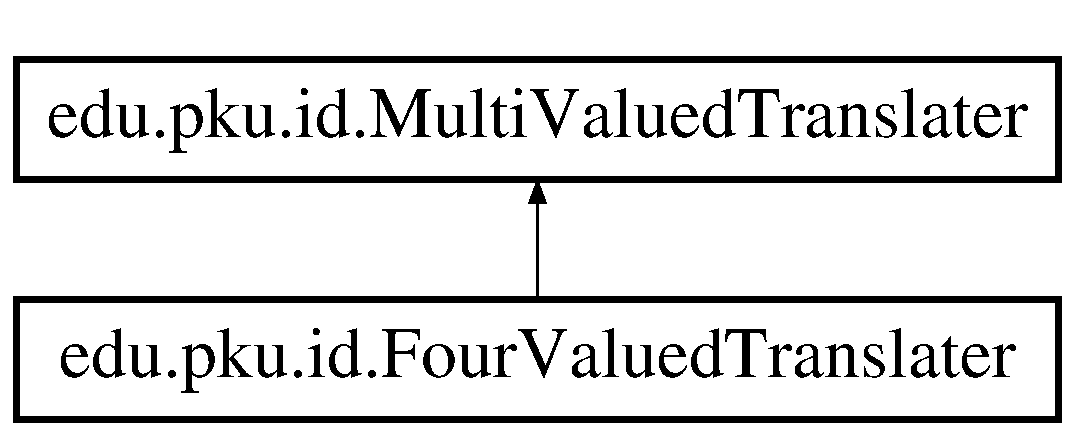
\includegraphics[height=2.000000cm]{classedu_1_1pku_1_1id_1_1_four_valued_translater}
\end{center}
\end{figure}
\subsection*{Public Member Functions}
\begin{DoxyCompactItemize}
\item 
\hyperlink{classedu_1_1pku_1_1id_1_1_four_valued_translater_acb79417b0c7fd741946b3d7f54e6825f}{FourValuedTranslater} ()
\item 
void \hyperlink{classedu_1_1pku_1_1id_1_1_four_valued_translater_a364637e20334ca6017ceffb49de3e551}{translate} ()
\item 
IVecInt \hyperlink{classedu_1_1pku_1_1id_1_1_four_valued_translater_acc8ee22b4ef34b8c596a5823521ffe03}{translateClause} (IVecInt clauseIn)
\end{DoxyCompactItemize}


\subsection{Constructor \& Destructor Documentation}
\hypertarget{classedu_1_1pku_1_1id_1_1_four_valued_translater_acb79417b0c7fd741946b3d7f54e6825f}{
\index{edu::pku::id::FourValuedTranslater@{edu::pku::id::FourValuedTranslater}!FourValuedTranslater@{FourValuedTranslater}}
\index{FourValuedTranslater@{FourValuedTranslater}!edu::pku::id::FourValuedTranslater@{edu::pku::id::FourValuedTranslater}}
\subsubsection[{FourValuedTranslater}]{\setlength{\rightskip}{0pt plus 5cm}edu.pku.id.FourValuedTranslater.FourValuedTranslater (
\begin{DoxyParamCaption}
{}
\end{DoxyParamCaption}
)}}
\label{classedu_1_1pku_1_1id_1_1_four_valued_translater_acb79417b0c7fd741946b3d7f54e6825f}


\subsection{Member Function Documentation}
\hypertarget{classedu_1_1pku_1_1id_1_1_four_valued_translater_a364637e20334ca6017ceffb49de3e551}{
\index{edu::pku::id::FourValuedTranslater@{edu::pku::id::FourValuedTranslater}!translate@{translate}}
\index{translate@{translate}!edu::pku::id::FourValuedTranslater@{edu::pku::id::FourValuedTranslater}}
\subsubsection[{translate}]{\setlength{\rightskip}{0pt plus 5cm}void edu.pku.id.FourValuedTranslater.translate (
\begin{DoxyParamCaption}
{}
\end{DoxyParamCaption}
)\hspace{0.3cm}{\ttfamily  \mbox{[}virtual\mbox{]}}}}
\label{classedu_1_1pku_1_1id_1_1_four_valued_translater_a364637e20334ca6017ceffb49de3e551}


Implements \hyperlink{classedu_1_1pku_1_1id_1_1_multi_valued_translater_a57e687a8b1c011fb7c0ccbd72272e328}{edu.pku.id.MultiValuedTranslater}.

\hypertarget{classedu_1_1pku_1_1id_1_1_four_valued_translater_acc8ee22b4ef34b8c596a5823521ffe03}{
\index{edu::pku::id::FourValuedTranslater@{edu::pku::id::FourValuedTranslater}!translateClause@{translateClause}}
\index{translateClause@{translateClause}!edu::pku::id::FourValuedTranslater@{edu::pku::id::FourValuedTranslater}}
\subsubsection[{translateClause}]{\setlength{\rightskip}{0pt plus 5cm}IVecInt edu.pku.id.FourValuedTranslater.translateClause (
\begin{DoxyParamCaption}
\item[{IVecInt}]{ clauseIn}
\end{DoxyParamCaption}
)}}
\label{classedu_1_1pku_1_1id_1_1_four_valued_translater_acc8ee22b4ef34b8c596a5823521ffe03}


The documentation for this class was generated from the following file:\begin{DoxyCompactItemize}
\item 
src/edu/pku/id/\hyperlink{_four_valued_translater_8java}{FourValuedTranslater.java}\end{DoxyCompactItemize}

\hypertarget{classgnu_1_1getopt_1_1_getopt}{
\section{gnu.getopt.Getopt Class Reference}
\label{classgnu_1_1getopt_1_1_getopt}\index{gnu::getopt::Getopt@{gnu::getopt::Getopt}}
}
\subsection*{Public Member Functions}
\begin{DoxyCompactItemize}
\item 
\hyperlink{classgnu_1_1getopt_1_1_getopt_a7babf5343414128369b45f7eb90882c1}{Getopt} (String \hyperlink{classgnu_1_1getopt_1_1_getopt_aef9686af24b220286d279467d2741a6d}{progname}, String\mbox{[}$\,$\mbox{]} \hyperlink{classgnu_1_1getopt_1_1_getopt_adde2117f0df42f3254b37b05fd9833cf}{argv}, String \hyperlink{classgnu_1_1getopt_1_1_getopt_a3a731b226188580b7cf0928b97d0502d}{optstring})
\item 
\hyperlink{classgnu_1_1getopt_1_1_getopt_a5953b9f2928dd3cb130d6a6767f4a613}{Getopt} (String \hyperlink{classgnu_1_1getopt_1_1_getopt_aef9686af24b220286d279467d2741a6d}{progname}, String\mbox{[}$\,$\mbox{]} \hyperlink{classgnu_1_1getopt_1_1_getopt_adde2117f0df42f3254b37b05fd9833cf}{argv}, String \hyperlink{classgnu_1_1getopt_1_1_getopt_a3a731b226188580b7cf0928b97d0502d}{optstring}, \hyperlink{classgnu_1_1getopt_1_1_long_opt}{LongOpt}\mbox{[}$\,$\mbox{]} \hyperlink{classgnu_1_1getopt_1_1_getopt_a5baa01494994d09203b475edd9c9eb98}{long\_\-options})
\item 
\hyperlink{classgnu_1_1getopt_1_1_getopt_aa28cedbcac63dcef002fefe837edc288}{Getopt} (String \hyperlink{classgnu_1_1getopt_1_1_getopt_aef9686af24b220286d279467d2741a6d}{progname}, String\mbox{[}$\,$\mbox{]} \hyperlink{classgnu_1_1getopt_1_1_getopt_adde2117f0df42f3254b37b05fd9833cf}{argv}, String \hyperlink{classgnu_1_1getopt_1_1_getopt_a3a731b226188580b7cf0928b97d0502d}{optstring}, \hyperlink{classgnu_1_1getopt_1_1_long_opt}{LongOpt}\mbox{[}$\,$\mbox{]} \hyperlink{classgnu_1_1getopt_1_1_getopt_a5baa01494994d09203b475edd9c9eb98}{long\_\-options}, boolean \hyperlink{classgnu_1_1getopt_1_1_getopt_a81e9a30f84d4dc8e7b28e1d1dcecbd4c}{long\_\-only})
\item 
void \hyperlink{classgnu_1_1getopt_1_1_getopt_a2cc4f71348a33281ee943cc20b0af90a}{setOptstring} (String \hyperlink{classgnu_1_1getopt_1_1_getopt_a3a731b226188580b7cf0928b97d0502d}{optstring})
\item 
int \hyperlink{classgnu_1_1getopt_1_1_getopt_af9f1a42a320e2112325fd5ea41504bdf}{getOptind} ()
\item 
void \hyperlink{classgnu_1_1getopt_1_1_getopt_a876a62ef42014ff4b18be4b132eb7ed8}{setOptind} (int \hyperlink{classgnu_1_1getopt_1_1_getopt_ae80c10d8bfc957fd93bec2f3619cbf18}{optind})
\item 
void \hyperlink{classgnu_1_1getopt_1_1_getopt_a9ac59fc870b6efdafee66014924cf12a}{setArgv} (String\mbox{[}$\,$\mbox{]} \hyperlink{classgnu_1_1getopt_1_1_getopt_adde2117f0df42f3254b37b05fd9833cf}{argv})
\item 
String \hyperlink{classgnu_1_1getopt_1_1_getopt_a306e1acd3be41f5e9462f42e78a6ca93}{getOptarg} ()
\item 
void \hyperlink{classgnu_1_1getopt_1_1_getopt_aa132089015be3665ca422f3eae3d0a38}{setOpterr} (boolean \hyperlink{classgnu_1_1getopt_1_1_getopt_a8712d370a08f90b7b49b0261a2df8581}{opterr})
\item 
int \hyperlink{classgnu_1_1getopt_1_1_getopt_ad33843ab06130ce60d60556241d1dc99}{getOptopt} ()
\item 
int \hyperlink{classgnu_1_1getopt_1_1_getopt_abaf4fb9de230e1950d93abc1b9f86a8d}{getLongind} ()
\item 
int \hyperlink{classgnu_1_1getopt_1_1_getopt_a49e6fc6e18756f5dfaf85c1067325c3b}{getopt} ()
\end{DoxyCompactItemize}
\subsection*{Protected Member Functions}
\begin{DoxyCompactItemize}
\item 
void \hyperlink{classgnu_1_1getopt_1_1_getopt_aaa3d697613ad3eacc714b9857dc52570}{exchange} (String\mbox{[}$\,$\mbox{]} \hyperlink{classgnu_1_1getopt_1_1_getopt_adde2117f0df42f3254b37b05fd9833cf}{argv})
\item 
int \hyperlink{classgnu_1_1getopt_1_1_getopt_ab748f7d3ed0781871d0b64f242e3674a}{checkLongOption} ()
\end{DoxyCompactItemize}
\subsection*{Protected Attributes}
\begin{DoxyCompactItemize}
\item 
String \hyperlink{classgnu_1_1getopt_1_1_getopt_a1b9f80db609f412ec4650ca9a8280882}{optarg}
\item 
int \hyperlink{classgnu_1_1getopt_1_1_getopt_ae80c10d8bfc957fd93bec2f3619cbf18}{optind} = 0
\item 
boolean \hyperlink{classgnu_1_1getopt_1_1_getopt_a8712d370a08f90b7b49b0261a2df8581}{opterr} = true
\item 
int \hyperlink{classgnu_1_1getopt_1_1_getopt_ac9bb6ef79a5d0467f38cdf2ac07c51ef}{optopt} = '?'
\item 
String \hyperlink{classgnu_1_1getopt_1_1_getopt_a94938d6f4baca982818fc56f9e9ee959}{nextchar}
\item 
String \hyperlink{classgnu_1_1getopt_1_1_getopt_a3a731b226188580b7cf0928b97d0502d}{optstring}
\item 
\hyperlink{classgnu_1_1getopt_1_1_long_opt}{LongOpt}\mbox{[}$\,$\mbox{]} \hyperlink{classgnu_1_1getopt_1_1_getopt_a5baa01494994d09203b475edd9c9eb98}{long\_\-options}
\item 
boolean \hyperlink{classgnu_1_1getopt_1_1_getopt_a81e9a30f84d4dc8e7b28e1d1dcecbd4c}{long\_\-only}
\item 
int \hyperlink{classgnu_1_1getopt_1_1_getopt_af0fee3aa183afb5b5326894bf0c25f64}{longind}
\item 
boolean \hyperlink{classgnu_1_1getopt_1_1_getopt_a2500f828284f39e5daf994a11be3ffe5}{posixly\_\-correct}
\item 
boolean \hyperlink{classgnu_1_1getopt_1_1_getopt_a156f519421b9d7707adee504e0bafac8}{longopt\_\-handled}
\item 
int \hyperlink{classgnu_1_1getopt_1_1_getopt_a2af5425ca486d7546c261d5f9f45ed26}{first\_\-nonopt} = 1
\item 
int \hyperlink{classgnu_1_1getopt_1_1_getopt_aaca077ce23c672df0a638fbb63898446}{last\_\-nonopt} = 1
\item 
String\mbox{[}$\,$\mbox{]} \hyperlink{classgnu_1_1getopt_1_1_getopt_adde2117f0df42f3254b37b05fd9833cf}{argv}
\item 
int \hyperlink{classgnu_1_1getopt_1_1_getopt_a9512cc64df132d096957ae7f24f5480d}{ordering}
\item 
String \hyperlink{classgnu_1_1getopt_1_1_getopt_aef9686af24b220286d279467d2741a6d}{progname}
\end{DoxyCompactItemize}
\subsection*{Static Protected Attributes}
\begin{DoxyCompactItemize}
\item 
static final int \hyperlink{classgnu_1_1getopt_1_1_getopt_a565d6f6705e2d2d1273ee1d5880a0073}{REQUIRE\_\-ORDER} = 1
\item 
static final int \hyperlink{classgnu_1_1getopt_1_1_getopt_a40d611d25b27cb29cc6f3791882652ab}{PERMUTE} = 2
\item 
static final int \hyperlink{classgnu_1_1getopt_1_1_getopt_a1c175740e7a8b309f46ac10259eeea11}{RETURN\_\-IN\_\-ORDER} = 3
\end{DoxyCompactItemize}
\subsection*{Private Attributes}
\begin{DoxyCompactItemize}
\item 
boolean \hyperlink{classgnu_1_1getopt_1_1_getopt_a852cfaf9571de753256f2edd920c6abc}{endparse} = false
\item 
ResourceBundle \hyperlink{classgnu_1_1getopt_1_1_getopt_a3abb4bdca8e36a53d49f71fb1c421512}{\_\-messages}
\end{DoxyCompactItemize}


\subsection{Detailed Description}
This is a Java port of GNU getopt, a class for parsing command line arguments passed to programs. It is based on the C \hyperlink{classgnu_1_1getopt_1_1_getopt_a49e6fc6e18756f5dfaf85c1067325c3b}{getopt()} functions in glibc 2.0.6 and should parse options in a 100\% compatible manner. If it does not, that is a bug. The programmer's interface is also very compatible. 

To use \hyperlink{classgnu_1_1getopt_1_1_getopt}{Getopt}, create a \hyperlink{classgnu_1_1getopt_1_1_getopt}{Getopt} object with a argv array passed to the main method, then call the \hyperlink{classgnu_1_1getopt_1_1_getopt_a49e6fc6e18756f5dfaf85c1067325c3b}{getopt()} method in a loop. It will return an int that contains the value of the option character parsed from the command line. When there are no more options to be parsed, it returns -\/1. 

A command line option can be defined to take an argument. If an option has an argument, the value of that argument is stored in an instance variable called optarg, which can be accessed using the \hyperlink{classgnu_1_1getopt_1_1_getopt_a306e1acd3be41f5e9462f42e78a6ca93}{getOptarg()} method. If an option that requires an argument is found, but there is no argument present, then an error message is printed. Normally \hyperlink{classgnu_1_1getopt_1_1_getopt_a49e6fc6e18756f5dfaf85c1067325c3b}{getopt()} returns a '?' in this situation, but that can be changed as described below. 

If an invalid option is encountered, an error message is printed to the standard error and \hyperlink{classgnu_1_1getopt_1_1_getopt_a49e6fc6e18756f5dfaf85c1067325c3b}{getopt()} returns a '?'. The value of the invalid option encountered is stored in the instance variable optopt which can be retrieved using the \hyperlink{classgnu_1_1getopt_1_1_getopt_ad33843ab06130ce60d60556241d1dc99}{getOptopt()} method. To suppress the printing of error messages for this or any other error, set the value of the opterr instance variable to false using the \hyperlink{classgnu_1_1getopt_1_1_getopt_aa132089015be3665ca422f3eae3d0a38}{setOpterr()} method. 

Between calls to \hyperlink{classgnu_1_1getopt_1_1_getopt_a49e6fc6e18756f5dfaf85c1067325c3b}{getopt()}, the instance variable optind is used to keep track of where the object is in the parsing process. After all options have been returned, optind is the index in argv of the first non-\/option argument. This variable can be accessed with the \hyperlink{classgnu_1_1getopt_1_1_getopt_af9f1a42a320e2112325fd5ea41504bdf}{getOptind()} method. 

Note that this object expects command line options to be passed in the traditional Unix manner. That is, proceeded by a '-\/' character. Multiple options can follow the '-\/'. For example \char`\"{}-\/abc\char`\"{} is equivalent to \char`\"{}-\/a -\/b -\/c\char`\"{}. If an option takes a required argument, the value of the argument can immediately follow the option character or be present in the next argv element. For example, \char`\"{}-\/cfoo\char`\"{} and \char`\"{}-\/c foo\char`\"{} both represent an option character of 'c' with an argument of \char`\"{}foo\char`\"{} assuming c takes a required argument. If an option takes an argument that is not required, then any argument must immediately follow the option character in the same argv element. For example, if c takes a non-\/required argument, then \char`\"{}-\/cfoo\char`\"{} represents option character 'c' with an argument of \char`\"{}foo\char`\"{} while \char`\"{}-\/c foo\char`\"{} represents the option character 'c' with no argument, and a first non-\/option argv element of \char`\"{}foo\char`\"{}. 

The user can stop \hyperlink{classgnu_1_1getopt_1_1_getopt_a49e6fc6e18756f5dfaf85c1067325c3b}{getopt()} from scanning any further into a command line by using the special argument \char`\"{}-\/-\/\char`\"{} by itself. For example: \char`\"{}-\/a -\/-\/ -\/d\char`\"{} would return an option character of 'a', then return -\/1 The \char`\"{}-\/-\/\char`\"{} is discarded and \char`\"{}-\/d\char`\"{} is pointed to by optind as the first non-\/option argv element. 

Here is a basic example of using \hyperlink{classgnu_1_1getopt_1_1_getopt}{Getopt}: 


\begin{DoxyPre}
 \hyperlink{classgnu_1_1getopt_1_1_getopt}{Getopt} g = new \hyperlink{classgnu_1_1getopt_1_1_getopt}{Getopt}("testprog", argv, "ab:c::d");
 //
 int c;
 String arg;
 while ((c = g.getopt()) != -1)
   \{
     switch(c)
       \{
          case 'a':
          case 'd':
            System.out.print("You picked " + (char)c + "\(\backslash\)n");
            break;
            //
          case 'b':
          case 'c':
            arg = g.getOptarg();
            System.out.print("You picked " + (char)c + 
                             " with an argument of " +
                             ((arg != null) ? arg : "null") + "\(\backslash\)n");
            break;
            //
          case '?':
            break; // \hyperlink{classgnu_1_1getopt_1_1_getopt_a49e6fc6e18756f5dfaf85c1067325c3b}{getopt()} already printed an error
            //
          default:
            System.out.print("getopt() returned " + c + "\(\backslash\)n");
       \}
   \}
 \end{DoxyPre}
 

In this example, a new \hyperlink{classgnu_1_1getopt_1_1_getopt}{Getopt} object is created with three params. The first param is the program name. This is for printing error messages in the form \char`\"{}program: error message\char`\"{}. In the C version, this value is taken from argv\mbox{[}0\mbox{]}, but in Java the program name is not passed in that element, thus the need for this parameter. The second param is the argument list that was passed to the main() method. The third param is the list of valid options. Each character represents a valid option. If the character is followed by a single colon, then that option has a required argument. If the character is followed by two colons, then that option has an argument that is not required. 

Note in this example that the value returned from \hyperlink{classgnu_1_1getopt_1_1_getopt_a49e6fc6e18756f5dfaf85c1067325c3b}{getopt()} is cast to a char prior to printing. This is required in order to make the value display correctly as a character instead of an integer. 

If the first character in the option string is a colon, for example \char`\"{}:abc::d\char`\"{}, then \hyperlink{classgnu_1_1getopt_1_1_getopt_a49e6fc6e18756f5dfaf85c1067325c3b}{getopt()} will return a ':' instead of a '?' when it encounters an option with a missing required argument. This allows the caller to distinguish between invalid options and valid options that are simply incomplete. 

In the traditional Unix \hyperlink{classgnu_1_1getopt_1_1_getopt_a49e6fc6e18756f5dfaf85c1067325c3b}{getopt()}, -\/1 is returned when the first non-\/option charcter is encountered. In GNU \hyperlink{classgnu_1_1getopt_1_1_getopt_a49e6fc6e18756f5dfaf85c1067325c3b}{getopt()}, the default behavior is to allow options to appear anywhere on the command line. The \hyperlink{classgnu_1_1getopt_1_1_getopt_a49e6fc6e18756f5dfaf85c1067325c3b}{getopt()} method permutes the argument to make it appear to the caller that all options were at the beginning of the command line, and all non-\/options were at the end. For example, calling \hyperlink{classgnu_1_1getopt_1_1_getopt_a49e6fc6e18756f5dfaf85c1067325c3b}{getopt()} with command line args of \char`\"{}-\/a foo bar -\/d\char`\"{} returns options 'a' and 'd', then sets optind to point to \char`\"{}foo\char`\"{}. The program would read the last two argv elements as \char`\"{}foo\char`\"{} and \char`\"{}bar\char`\"{}, just as if the user had typed \char`\"{}-\/a -\/d foo bar\char`\"{}. 

The user can force \hyperlink{classgnu_1_1getopt_1_1_getopt_a49e6fc6e18756f5dfaf85c1067325c3b}{getopt()} to stop scanning the command line with the special argument \char`\"{}-\/-\/\char`\"{} by itself. Any elements occuring before the \char`\"{}-\/-\/\char`\"{} are scanned and permuted as normal. Any elements after the \char`\"{}-\/-\/\char`\"{} are returned as is as non-\/option argv elements. For example, \char`\"{}foo -\/a -\/-\/ bar -\/d\char`\"{} would return option 'a' then -\/1. optind would point to \char`\"{}foo\char`\"{}, \char`\"{}bar\char`\"{} and \char`\"{}-\/d\char`\"{} as the non-\/option argv elements. The \char`\"{}-\/-\/\char`\"{} is discarded by \hyperlink{classgnu_1_1getopt_1_1_getopt_a49e6fc6e18756f5dfaf85c1067325c3b}{getopt()}. 

There are two ways this default behavior can be modified. The first is to specify traditional Unix \hyperlink{classgnu_1_1getopt_1_1_getopt_a49e6fc6e18756f5dfaf85c1067325c3b}{getopt()} behavior (which is also POSIX behavior) in which scanning stops when the first non-\/option argument encountered. (Thus \char`\"{}-\/a foo bar -\/d\char`\"{} would return 'a' as an option and have \char`\"{}foo\char`\"{}, \char`\"{}bar\char`\"{}, and \char`\"{}-\/d\char`\"{} as non-\/option elements). The second is to allow options anywhere, but to return all elements in the order they occur on the command line. When a non-\/option element is ecountered, an integer 1 is returned and the value of the non-\/option element is stored in optarg is if it were the argument to that option. For example, \char`\"{}-\/a foo -\/d\char`\"{}, returns first 'a', then 1 (with optarg set to \char`\"{}foo\char`\"{}) then 'd' then -\/1. When this \char`\"{}return in order\char`\"{} functionality is enabled, the only way to stop \hyperlink{classgnu_1_1getopt_1_1_getopt_a49e6fc6e18756f5dfaf85c1067325c3b}{getopt()} from scanning all command line elements is to use the special \char`\"{}-\/-\/\char`\"{} string by itself as described above. An example is \char`\"{}-\/a foo -\/b -\/-\/ bar\char`\"{}, which would return 'a', then integer 1 with optarg set to \char`\"{}foo\char`\"{}, then 'b', then -\/1. optind would then point to \char`\"{}bar\char`\"{} as the first non-\/option argv element. The \char`\"{}-\/-\/\char`\"{} is discarded. 

The POSIX/traditional behavior is enabled by either setting the property \char`\"{}gnu.posixly\_\-correct\char`\"{} or by putting a '+' sign as the first character of the option string. The difference between the two methods is that setting the gnu.posixly\_\-correct property also forces certain error messages to be displayed in POSIX format. To enable the \char`\"{}return in order\char`\"{} functionality, put a '-\/' as the first character of the option string. Note that after determining the proper behavior, \hyperlink{classgnu_1_1getopt_1_1_getopt}{Getopt} strips this leading '+' or '-\/', meaning that a ':' placed as the second character after one of those two will still cause \hyperlink{classgnu_1_1getopt_1_1_getopt_a49e6fc6e18756f5dfaf85c1067325c3b}{getopt()} to return a ':' instead of a '?' if a required option argument is missing. 

In addition to traditional single character options, GNU \hyperlink{classgnu_1_1getopt_1_1_getopt}{Getopt} also supports long options. These are preceeded by a \char`\"{}-\/-\/\char`\"{} sequence and can be as long as desired. Long options provide a more user-\/friendly way of entering command line options. For example, in addition to a \char`\"{}-\/h\char`\"{} for help, a program could support also \char`\"{}-\/-\/help\char`\"{}. 

Like short options, long options can also take a required or non-\/required argument. Required arguments can either be specified by placing an equals sign after the option name, then the argument, or by putting the argument in the next argv element. For example: \char`\"{}-\/-\/outputdir=foo\char`\"{} and \char`\"{}-\/-\/outputdir foo\char`\"{} both represent an option of \char`\"{}outputdir\char`\"{} with an argument of \char`\"{}foo\char`\"{}, assuming that outputdir takes a required argument. If a long option takes a non-\/required argument, then the equals sign form must be used to specify the argument. In this case, \char`\"{}-\/-\/outputdir=foo\char`\"{} would represent option outputdir with an argument of \char`\"{}foo\char`\"{} while \char`\"{}-\/-\/outputdir foo\char`\"{} would represent the option outputdir with no argument and a first non-\/option argv element of \char`\"{}foo\char`\"{}. 

Long options can also be specified using a special POSIX argument format (one that I highly discourage). This form of entry is enabled by placing a \char`\"{}W;\char`\"{} (yes, 'W' then a semi-\/colon) in the valid option string. This causes getopt to treat the name following the \char`\"{}-\/W\char`\"{} as the name of the long option. For example, \char`\"{}-\/W outputdir=foo\char`\"{} would be equivalent to \char`\"{}-\/-\/outputdir=foo\char`\"{}. The name can immediately follow the \char`\"{}-\/W\char`\"{} like so: \char`\"{}-\/Woutputdir=foo\char`\"{}. Option arguments are handled identically to normal long options. If a string follows the \char`\"{}-\/W\char`\"{} that does not represent a valid long option, then \hyperlink{classgnu_1_1getopt_1_1_getopt_a49e6fc6e18756f5dfaf85c1067325c3b}{getopt()} returns 'W' and the caller must decide what to do. Otherwise \hyperlink{classgnu_1_1getopt_1_1_getopt_a49e6fc6e18756f5dfaf85c1067325c3b}{getopt()} returns a long option value as described below. 

While long options offer convenience, they can also be tedious to type in full. So it is permissible to abbreviate the option name to as few characters as required to uniquely identify it. If the name can represent multiple long options, then an error message is printed and \hyperlink{classgnu_1_1getopt_1_1_getopt_a49e6fc6e18756f5dfaf85c1067325c3b}{getopt()} returns a '?'. 

If an invalid option is specified or a required option argument is missing, \hyperlink{classgnu_1_1getopt_1_1_getopt_a49e6fc6e18756f5dfaf85c1067325c3b}{getopt()} prints an error and returns a '?' or ':' exactly as for short options. Note that when an invalid long option is encountered, the optopt variable is set to integer 0 and so cannot be used to identify the incorrect option the user entered. 

Long options are defined by \hyperlink{classgnu_1_1getopt_1_1_long_opt}{LongOpt} objects. These objects are created with a contructor that takes four params: a String representing the object name, a integer specifying what arguments the option takes (the value is one of \hyperlink{classgnu_1_1getopt_1_1_long_opt_a5af856e8de6a5f528d4da2b8706f7abe}{LongOpt.NO\_\-ARGUMENT}, \hyperlink{classgnu_1_1getopt_1_1_long_opt_a8105c98436b46a0b4de39a3afab230c2}{LongOpt.REQUIRED\_\-ARGUMENT}, or \hyperlink{classgnu_1_1getopt_1_1_long_opt_a31819aae074fa1d80f547817640b31c1}{LongOpt.OPTIONAL\_\-ARGUMENT}), a StringBuffer flag object (described below), and an integer value (described below). 

To enable long option parsing, create an array of LongOpt's representing the legal options and pass it to the \hyperlink{classgnu_1_1getopt_1_1_getopt_a7babf5343414128369b45f7eb90882c1}{Getopt()} constructor. WARNING: If all elements of the array are not populated with \hyperlink{classgnu_1_1getopt_1_1_long_opt}{LongOpt} objects, the \hyperlink{classgnu_1_1getopt_1_1_getopt_a49e6fc6e18756f5dfaf85c1067325c3b}{getopt()} method will throw a NullPointerException. 

When \hyperlink{classgnu_1_1getopt_1_1_getopt_a49e6fc6e18756f5dfaf85c1067325c3b}{getopt()} is called and a long option is encountered, one of two things can be returned. If the flag field in the \hyperlink{classgnu_1_1getopt_1_1_long_opt}{LongOpt} object representing the long option is non-\/null, then the integer value field is stored there and an integer 0 is returned to the caller. The val field can then be retrieved from the flag field. Note that since the flag field is a StringBuffer, the appropriate String to integer converions must be performed in order to get the actual int value stored there. If the flag field in the \hyperlink{classgnu_1_1getopt_1_1_long_opt}{LongOpt} object is null, then the value field of the \hyperlink{classgnu_1_1getopt_1_1_long_opt}{LongOpt} is returned. This can be the character of a short option. This allows an app to have both a long and short option sequence (say, \char`\"{}-\/h\char`\"{} and \char`\"{}-\/-\/help\char`\"{}) that do the exact same thing. 

With long options, there is an alternative method of determining which option was selected. The method \hyperlink{classgnu_1_1getopt_1_1_getopt_abaf4fb9de230e1950d93abc1b9f86a8d}{getLongind()} will return the the index in the long option array (NOT argv) of the long option found. So if multiple long options are configured to return the same value, the application can use \hyperlink{classgnu_1_1getopt_1_1_getopt_abaf4fb9de230e1950d93abc1b9f86a8d}{getLongind()} to distinguish between them. 

Here is an expanded \hyperlink{classgnu_1_1getopt_1_1_getopt}{Getopt} example using long options and various techniques described above: 


\begin{DoxyPre}
 int c;
 String arg;
 \hyperlink{classgnu_1_1getopt_1_1_long_opt}{LongOpt}[] longopts = new \hyperlink{classgnu_1_1getopt_1_1_long_opt}{LongOpt}[3];
 // 
 StringBuffer sb = new StringBuffer();
 longopts[0] = new \hyperlink{classgnu_1_1getopt_1_1_long_opt}{LongOpt}("help", \hyperlink{classgnu_1_1getopt_1_1_long_opt_a5af856e8de6a5f528d4da2b8706f7abe}{LongOpt.NO\_ARGUMENT}, null, 'h');
 longopts[1] = new \hyperlink{classgnu_1_1getopt_1_1_long_opt}{LongOpt}("outputdir", \hyperlink{classgnu_1_1getopt_1_1_long_opt_a8105c98436b46a0b4de39a3afab230c2}{LongOpt.REQUIRED\_ARGUMENT}, sb, 'o'); 
 longopts[2] = new \hyperlink{classgnu_1_1getopt_1_1_long_opt}{LongOpt}("maximum", \hyperlink{classgnu_1_1getopt_1_1_long_opt_a31819aae074fa1d80f547817640b31c1}{LongOpt.OPTIONAL\_ARGUMENT}, null, 2);
 // 
 \hyperlink{classgnu_1_1getopt_1_1_getopt}{Getopt} g = new \hyperlink{classgnu_1_1getopt_1_1_getopt}{Getopt}("testprog", argv, "-:bc::d:hW;", longopts);
 g.setOpterr(false); // We'll do our own error handling
 //
 while ((c = g.getopt()) != -1)
   switch (c)
     \{
        case 0:
          arg = g.getOptarg();
          System.out.println("Got long option with value '" +
                             (char)(new Integer(sb.toString())).intValue()
                             + "' with argument " +
                             ((arg != null) ? arg : "null"));
          break;
          //
        case 1:
          System.out.println("I see you have return in order set and that " +
                             "a non-option argv element was just found " +
                             "with the value '" + g.getOptarg() + "'");
          break;
          //
        case 2:
          arg = g.getOptarg();
          System.out.println("I know this, but pretend I didn't");
          System.out.println("We picked option " +
                             longopts[g.getLongind()].getName() +
                           " with value " + 
                           ((arg != null) ? arg : "null"));
          break;
          //
        case 'b':
          System.out.println("You picked plain old option " + (char)c);
          break;
          //
        case 'c':
        case 'd':
          arg = g.getOptarg();
          System.out.println("You picked option '" + (char)c + 
                             "' with argument " +
                             ((arg != null) ? arg : "null"));
          break;
          //
        case 'h':
          System.out.println("I see you asked for help");
          break;
          //
        case 'W':
          System.out.println("Hmmm. You tried a -W with an incorrect long " +
                             "option name");
          break;
          //
        case ':':
          System.out.println("Doh! You need an argument for option " +
                             (char)g.getOptopt());
          break;
          //
        case '?':
          System.out.println("The option '" + (char)g.getOptopt() + 
                           "' is not valid");
          break;
          //
        default:
          System.out.println("getopt() returned " + c);
          break;
     \}
 //
 for (int i = g.getOptind(); i < argv.length ; i++)
   System.out.println("Non option argv element: " + argv[i] + "\(\backslash\)n");
 \end{DoxyPre}
 

There is an alternative form of the constructor used for long options above. This takes a trailing boolean flag. If set to false, \hyperlink{classgnu_1_1getopt_1_1_getopt}{Getopt} performs identically to the example, but if the boolean flag is true then long options are allowed to start with a single '-\/' instead of \char`\"{}-\/-\/\char`\"{}. If the first character of the option is a valid short option character, then the option is treated as if it were the short option. Otherwise it behaves as if the option is a long option. Note that the name given to this option -\/ long\_\-only -\/ is very counter-\/intuitive. It does not cause only long options to be parsed but instead enables the behavior described above. 

Note that the functionality and variable names used are driven from the C lib version as this object is a port of the C code, not a new implementation. This should aid in porting existing C/C++ code, as well as helping programmers familiar with the glibc version to adapt to the Java version even if it seems very non-\/Java at times. 

In this release I made all instance variables protected due to overwhelming public demand. Any code which relied on optarg, opterr, optind, or optopt being public will need to be modified to use the appropriate access methods. 

Please send all bug reports, requests, and comments to \href{mailto:arenn@urbanophile.com}{\tt arenn@urbanophile.com}.

\begin{DoxyVersion}{Version}
1.0.7
\end{DoxyVersion}
\begin{DoxyAuthor}{Author}
Roland McGrath (\href{mailto:roland@gnu.ai.mit.edu}{\tt roland@gnu.ai.mit.edu}) 

Ulrich Drepper (\href{mailto:drepper@cygnus.com}{\tt drepper@cygnus.com}) 

Aaron M. Renn (\href{mailto:arenn@urbanophile.com}{\tt arenn@urbanophile.com})
\end{DoxyAuthor}
\begin{DoxySeeAlso}{See also}
\hyperlink{classgnu_1_1getopt_1_1_long_opt}{LongOpt} 
\end{DoxySeeAlso}


\subsection{Constructor \& Destructor Documentation}
\hypertarget{classgnu_1_1getopt_1_1_getopt_a7babf5343414128369b45f7eb90882c1}{
\index{gnu::getopt::Getopt@{gnu::getopt::Getopt}!Getopt@{Getopt}}
\index{Getopt@{Getopt}!gnu::getopt::Getopt@{gnu::getopt::Getopt}}
\subsubsection[{Getopt}]{\setlength{\rightskip}{0pt plus 5cm}gnu.getopt.Getopt.Getopt (
\begin{DoxyParamCaption}
\item[{String}]{ progname, }
\item[{String\mbox{[}$\,$\mbox{]}}]{ argv, }
\item[{String}]{ optstring}
\end{DoxyParamCaption}
)}}
\label{classgnu_1_1getopt_1_1_getopt_a7babf5343414128369b45f7eb90882c1}
Construct a basic \hyperlink{classgnu_1_1getopt_1_1_getopt}{Getopt} instance with the given input data. Note that this handles \char`\"{}short\char`\"{} options only.


\begin{DoxyParams}{Parameters}
{\em progname} & The name to display as the program name when printing errors \\
\hline
{\em argv} & The String array passed as the command line to the program. \\
\hline
{\em optstring} & A String containing a description of the valid args for this program \\
\hline
\end{DoxyParams}
\hypertarget{classgnu_1_1getopt_1_1_getopt_a5953b9f2928dd3cb130d6a6767f4a613}{
\index{gnu::getopt::Getopt@{gnu::getopt::Getopt}!Getopt@{Getopt}}
\index{Getopt@{Getopt}!gnu::getopt::Getopt@{gnu::getopt::Getopt}}
\subsubsection[{Getopt}]{\setlength{\rightskip}{0pt plus 5cm}gnu.getopt.Getopt.Getopt (
\begin{DoxyParamCaption}
\item[{String}]{ progname, }
\item[{String\mbox{[}$\,$\mbox{]}}]{ argv, }
\item[{String}]{ optstring, }
\item[{{\bf LongOpt}\mbox{[}$\,$\mbox{]}}]{ long\_\-options}
\end{DoxyParamCaption}
)}}
\label{classgnu_1_1getopt_1_1_getopt_a5953b9f2928dd3cb130d6a6767f4a613}
Construct a \hyperlink{classgnu_1_1getopt_1_1_getopt}{Getopt} instance with given input data that is capable of parsing long options as well as short.


\begin{DoxyParams}{Parameters}
{\em progname} & The name to display as the program name when printing errors \\
\hline
{\em argv} & The String array passed as the command ilne to the program \\
\hline
{\em optstring} & A String containing a description of the valid short args for this program \\
\hline
{\em long\_\-options} & An array of \hyperlink{classgnu_1_1getopt_1_1_long_opt}{LongOpt} objects that describes the valid long args for this program \\
\hline
\end{DoxyParams}
\hypertarget{classgnu_1_1getopt_1_1_getopt_aa28cedbcac63dcef002fefe837edc288}{
\index{gnu::getopt::Getopt@{gnu::getopt::Getopt}!Getopt@{Getopt}}
\index{Getopt@{Getopt}!gnu::getopt::Getopt@{gnu::getopt::Getopt}}
\subsubsection[{Getopt}]{\setlength{\rightskip}{0pt plus 5cm}gnu.getopt.Getopt.Getopt (
\begin{DoxyParamCaption}
\item[{String}]{ progname, }
\item[{String\mbox{[}$\,$\mbox{]}}]{ argv, }
\item[{String}]{ optstring, }
\item[{{\bf LongOpt}\mbox{[}$\,$\mbox{]}}]{ long\_\-options, }
\item[{boolean}]{ long\_\-only}
\end{DoxyParamCaption}
)}}
\label{classgnu_1_1getopt_1_1_getopt_aa28cedbcac63dcef002fefe837edc288}
Construct a \hyperlink{classgnu_1_1getopt_1_1_getopt}{Getopt} instance with given input data that is capable of parsing long options and short options. Contrary to what you might think, the flag 'long\_\-only' does not determine whether or not we scan for only long arguments. Instead, a value of true here allows long arguments to start with a '-\/' instead of '-\/-\/' unless there is a conflict with a short option name.


\begin{DoxyParams}{Parameters}
{\em progname} & The name to display as the program name when printing errors \\
\hline
{\em argv} & The String array passed as the command ilne to the program \\
\hline
{\em optstring} & A String containing a description of the valid short args for this program \\
\hline
{\em long\_\-options} & An array of \hyperlink{classgnu_1_1getopt_1_1_long_opt}{LongOpt} objects that describes the valid long args for this program \\
\hline
{\em long\_\-only} & true if long options that do not conflict with short options can start with a '-\/' as well as '-\/-\/' \\
\hline
\end{DoxyParams}


\subsection{Member Function Documentation}
\hypertarget{classgnu_1_1getopt_1_1_getopt_ab748f7d3ed0781871d0b64f242e3674a}{
\index{gnu::getopt::Getopt@{gnu::getopt::Getopt}!checkLongOption@{checkLongOption}}
\index{checkLongOption@{checkLongOption}!gnu::getopt::Getopt@{gnu::getopt::Getopt}}
\subsubsection[{checkLongOption}]{\setlength{\rightskip}{0pt plus 5cm}int gnu.getopt.Getopt.checkLongOption (
\begin{DoxyParamCaption}
{}
\end{DoxyParamCaption}
)\hspace{0.3cm}{\ttfamily  \mbox{[}protected\mbox{]}}}}
\label{classgnu_1_1getopt_1_1_getopt_ab748f7d3ed0781871d0b64f242e3674a}
Check to see if an option is a valid long option. Called by \hyperlink{classgnu_1_1getopt_1_1_getopt_a49e6fc6e18756f5dfaf85c1067325c3b}{getopt()}. Put in a separate method because this needs to be done twice. (The C getopt authors just copy-\/pasted the code!).


\begin{DoxyParams}{Parameters}
{\em longind} & A buffer in which to store the 'val' field of found \hyperlink{classgnu_1_1getopt_1_1_long_opt}{LongOpt}\\
\hline
\end{DoxyParams}
\begin{DoxyReturn}{Returns}
Various things depending on circumstances 
\end{DoxyReturn}
\hypertarget{classgnu_1_1getopt_1_1_getopt_aaa3d697613ad3eacc714b9857dc52570}{
\index{gnu::getopt::Getopt@{gnu::getopt::Getopt}!exchange@{exchange}}
\index{exchange@{exchange}!gnu::getopt::Getopt@{gnu::getopt::Getopt}}
\subsubsection[{exchange}]{\setlength{\rightskip}{0pt plus 5cm}void gnu.getopt.Getopt.exchange (
\begin{DoxyParamCaption}
\item[{String\mbox{[}$\,$\mbox{]}}]{ argv}
\end{DoxyParamCaption}
)\hspace{0.3cm}{\ttfamily  \mbox{[}protected\mbox{]}}}}
\label{classgnu_1_1getopt_1_1_getopt_aaa3d697613ad3eacc714b9857dc52570}
Exchange the shorter segment with the far end of the longer segment. That puts the shorter segment into the right place. It leaves the longer segment in the right place overall, but it consists of two parts that need to be swapped next. This method is used by \hyperlink{classgnu_1_1getopt_1_1_getopt_a49e6fc6e18756f5dfaf85c1067325c3b}{getopt()} for argument permutation. \hypertarget{classgnu_1_1getopt_1_1_getopt_abaf4fb9de230e1950d93abc1b9f86a8d}{
\index{gnu::getopt::Getopt@{gnu::getopt::Getopt}!getLongind@{getLongind}}
\index{getLongind@{getLongind}!gnu::getopt::Getopt@{gnu::getopt::Getopt}}
\subsubsection[{getLongind}]{\setlength{\rightskip}{0pt plus 5cm}int gnu.getopt.Getopt.getLongind (
\begin{DoxyParamCaption}
{}
\end{DoxyParamCaption}
)}}
\label{classgnu_1_1getopt_1_1_getopt_abaf4fb9de230e1950d93abc1b9f86a8d}
Returns the index into the array of long options (NOT argv) representing the long option that was found. \hypertarget{classgnu_1_1getopt_1_1_getopt_a49e6fc6e18756f5dfaf85c1067325c3b}{
\index{gnu::getopt::Getopt@{gnu::getopt::Getopt}!getopt@{getopt}}
\index{getopt@{getopt}!gnu::getopt::Getopt@{gnu::getopt::Getopt}}
\subsubsection[{getopt}]{\setlength{\rightskip}{0pt plus 5cm}int gnu.getopt.Getopt.getopt (
\begin{DoxyParamCaption}
{}
\end{DoxyParamCaption}
)}}
\label{classgnu_1_1getopt_1_1_getopt_a49e6fc6e18756f5dfaf85c1067325c3b}
This method returns a char that is the current option that has been parsed from the command line. If the option takes an argument, then the internal variable 'optarg' is set which is a String representing the the value of the argument. This value can be retrieved by the caller using the \hyperlink{classgnu_1_1getopt_1_1_getopt_a306e1acd3be41f5e9462f42e78a6ca93}{getOptarg()} method. If an invalid option is found, an error message is printed and a '?' is returned. The name of the invalid option character can be retrieved by calling the \hyperlink{classgnu_1_1getopt_1_1_getopt_ad33843ab06130ce60d60556241d1dc99}{getOptopt()} method. When there are no more options to be scanned, this method returns -\/1. The index of first non-\/option element in argv can be retrieved with the \hyperlink{classgnu_1_1getopt_1_1_getopt_af9f1a42a320e2112325fd5ea41504bdf}{getOptind()} method.

\begin{DoxyReturn}{Returns}
Various things as described above 
\end{DoxyReturn}
\hypertarget{classgnu_1_1getopt_1_1_getopt_a306e1acd3be41f5e9462f42e78a6ca93}{
\index{gnu::getopt::Getopt@{gnu::getopt::Getopt}!getOptarg@{getOptarg}}
\index{getOptarg@{getOptarg}!gnu::getopt::Getopt@{gnu::getopt::Getopt}}
\subsubsection[{getOptarg}]{\setlength{\rightskip}{0pt plus 5cm}String gnu.getopt.Getopt.getOptarg (
\begin{DoxyParamCaption}
{}
\end{DoxyParamCaption}
)}}
\label{classgnu_1_1getopt_1_1_getopt_a306e1acd3be41f5e9462f42e78a6ca93}
For communication from `getopt' to the caller. When `getopt' finds an option that takes an argument, the argument value is returned here. Also, when `ordering' is RETURN\_\-IN\_\-ORDER, each non-\/option ARGV-\/element is returned here. No set method is provided because setting this variable has no effect. \hypertarget{classgnu_1_1getopt_1_1_getopt_af9f1a42a320e2112325fd5ea41504bdf}{
\index{gnu::getopt::Getopt@{gnu::getopt::Getopt}!getOptind@{getOptind}}
\index{getOptind@{getOptind}!gnu::getopt::Getopt@{gnu::getopt::Getopt}}
\subsubsection[{getOptind}]{\setlength{\rightskip}{0pt plus 5cm}int gnu.getopt.Getopt.getOptind (
\begin{DoxyParamCaption}
{}
\end{DoxyParamCaption}
)}}
\label{classgnu_1_1getopt_1_1_getopt_af9f1a42a320e2112325fd5ea41504bdf}
optind it the index in ARGV of the next element to be scanned. This is used for communication to and from the caller and for communication between successive calls to `getopt'.

When `getopt' returns -\/1, this is the index of the first of the non-\/option elements that the caller should itself scan.

Otherwise, `optind' communicates from one call to the next how much of ARGV has been scanned so far. \hypertarget{classgnu_1_1getopt_1_1_getopt_ad33843ab06130ce60d60556241d1dc99}{
\index{gnu::getopt::Getopt@{gnu::getopt::Getopt}!getOptopt@{getOptopt}}
\index{getOptopt@{getOptopt}!gnu::getopt::Getopt@{gnu::getopt::Getopt}}
\subsubsection[{getOptopt}]{\setlength{\rightskip}{0pt plus 5cm}int gnu.getopt.Getopt.getOptopt (
\begin{DoxyParamCaption}
{}
\end{DoxyParamCaption}
)}}
\label{classgnu_1_1getopt_1_1_getopt_ad33843ab06130ce60d60556241d1dc99}
When \hyperlink{classgnu_1_1getopt_1_1_getopt_a49e6fc6e18756f5dfaf85c1067325c3b}{getopt()} encounters an invalid option, it stores the value of that option in optopt which can be retrieved with this method. There is no corresponding set method because setting this variable has no effect. \hypertarget{classgnu_1_1getopt_1_1_getopt_a9ac59fc870b6efdafee66014924cf12a}{
\index{gnu::getopt::Getopt@{gnu::getopt::Getopt}!setArgv@{setArgv}}
\index{setArgv@{setArgv}!gnu::getopt::Getopt@{gnu::getopt::Getopt}}
\subsubsection[{setArgv}]{\setlength{\rightskip}{0pt plus 5cm}void gnu.getopt.Getopt.setArgv (
\begin{DoxyParamCaption}
\item[{String\mbox{[}$\,$\mbox{]}}]{ argv}
\end{DoxyParamCaption}
)}}
\label{classgnu_1_1getopt_1_1_getopt_a9ac59fc870b6efdafee66014924cf12a}
Since in GNU \hyperlink{classgnu_1_1getopt_1_1_getopt_a49e6fc6e18756f5dfaf85c1067325c3b}{getopt()} the argument vector is passed back in to the function every time, the caller can swap out argv on the fly. Since passing argv is not required in the Java version, this method allows the user to override argv. Note that incorrect use of this method can lead to serious lossage.


\begin{DoxyParams}{Parameters}
{\em argv} & New argument list \\
\hline
\end{DoxyParams}
\hypertarget{classgnu_1_1getopt_1_1_getopt_aa132089015be3665ca422f3eae3d0a38}{
\index{gnu::getopt::Getopt@{gnu::getopt::Getopt}!setOpterr@{setOpterr}}
\index{setOpterr@{setOpterr}!gnu::getopt::Getopt@{gnu::getopt::Getopt}}
\subsubsection[{setOpterr}]{\setlength{\rightskip}{0pt plus 5cm}void gnu.getopt.Getopt.setOpterr (
\begin{DoxyParamCaption}
\item[{boolean}]{ opterr}
\end{DoxyParamCaption}
)}}
\label{classgnu_1_1getopt_1_1_getopt_aa132089015be3665ca422f3eae3d0a38}
Normally \hyperlink{classgnu_1_1getopt_1_1_getopt}{Getopt} will print a message to the standard error when an invalid option is encountered. This can be suppressed (or re-\/enabled) by calling this method. There is no get method for this variable because if you can't remember the state you set this to, why should I? \hypertarget{classgnu_1_1getopt_1_1_getopt_a876a62ef42014ff4b18be4b132eb7ed8}{
\index{gnu::getopt::Getopt@{gnu::getopt::Getopt}!setOptind@{setOptind}}
\index{setOptind@{setOptind}!gnu::getopt::Getopt@{gnu::getopt::Getopt}}
\subsubsection[{setOptind}]{\setlength{\rightskip}{0pt plus 5cm}void gnu.getopt.Getopt.setOptind (
\begin{DoxyParamCaption}
\item[{int}]{ optind}
\end{DoxyParamCaption}
)}}
\label{classgnu_1_1getopt_1_1_getopt_a876a62ef42014ff4b18be4b132eb7ed8}
This method allows the optind index to be set manually. Normally this is not necessary (and incorrect usage of this method can lead to serious lossage), but optind is a public symbol in GNU getopt, so this method was added to allow it to be modified by the caller if desired.


\begin{DoxyParams}{Parameters}
{\em optind} & The new value of optind \\
\hline
\end{DoxyParams}
\hypertarget{classgnu_1_1getopt_1_1_getopt_a2cc4f71348a33281ee943cc20b0af90a}{
\index{gnu::getopt::Getopt@{gnu::getopt::Getopt}!setOptstring@{setOptstring}}
\index{setOptstring@{setOptstring}!gnu::getopt::Getopt@{gnu::getopt::Getopt}}
\subsubsection[{setOptstring}]{\setlength{\rightskip}{0pt plus 5cm}void gnu.getopt.Getopt.setOptstring (
\begin{DoxyParamCaption}
\item[{String}]{ optstring}
\end{DoxyParamCaption}
)}}
\label{classgnu_1_1getopt_1_1_getopt_a2cc4f71348a33281ee943cc20b0af90a}
In GNU getopt, it is possible to change the string containg valid options on the fly because it is passed as an argument to \hyperlink{classgnu_1_1getopt_1_1_getopt_a49e6fc6e18756f5dfaf85c1067325c3b}{getopt()} each time. In this version we do not pass the string on every call. In order to allow dynamic option string changing, this method is provided.


\begin{DoxyParams}{Parameters}
{\em optstring} & The new option string to use \\
\hline
\end{DoxyParams}


\subsection{Member Data Documentation}
\hypertarget{classgnu_1_1getopt_1_1_getopt_a3abb4bdca8e36a53d49f71fb1c421512}{
\index{gnu::getopt::Getopt@{gnu::getopt::Getopt}!\_\-messages@{\_\-messages}}
\index{\_\-messages@{\_\-messages}!gnu::getopt::Getopt@{gnu::getopt::Getopt}}
\subsubsection[{\_\-messages}]{\setlength{\rightskip}{0pt plus 5cm}ResourceBundle {\bf gnu.getopt.Getopt.\_\-messages}\hspace{0.3cm}{\ttfamily  \mbox{[}private\mbox{]}}}}
\label{classgnu_1_1getopt_1_1_getopt_a3abb4bdca8e36a53d49f71fb1c421512}
{\bfseries Initial value:}
\begin{DoxyCode}
 PropertyResourceBundle.getBundle(
                           "gnu/getopt/MessagesBundle", Locale.getDefault())
\end{DoxyCode}
The localized strings are kept in a separate file \hypertarget{classgnu_1_1getopt_1_1_getopt_adde2117f0df42f3254b37b05fd9833cf}{
\index{gnu::getopt::Getopt@{gnu::getopt::Getopt}!argv@{argv}}
\index{argv@{argv}!gnu::getopt::Getopt@{gnu::getopt::Getopt}}
\subsubsection[{argv}]{\setlength{\rightskip}{0pt plus 5cm}String \mbox{[}$\,$\mbox{]} {\bf gnu.getopt.Getopt.argv}\hspace{0.3cm}{\ttfamily  \mbox{[}protected\mbox{]}}}}
\label{classgnu_1_1getopt_1_1_getopt_adde2117f0df42f3254b37b05fd9833cf}
Saved argument list passed to the program \hypertarget{classgnu_1_1getopt_1_1_getopt_a852cfaf9571de753256f2edd920c6abc}{
\index{gnu::getopt::Getopt@{gnu::getopt::Getopt}!endparse@{endparse}}
\index{endparse@{endparse}!gnu::getopt::Getopt@{gnu::getopt::Getopt}}
\subsubsection[{endparse}]{\setlength{\rightskip}{0pt plus 5cm}boolean {\bf gnu.getopt.Getopt.endparse} = false\hspace{0.3cm}{\ttfamily  \mbox{[}private\mbox{]}}}}
\label{classgnu_1_1getopt_1_1_getopt_a852cfaf9571de753256f2edd920c6abc}
Flag to tell getopt to immediately return -\/1 the next time it is called. \hypertarget{classgnu_1_1getopt_1_1_getopt_a2af5425ca486d7546c261d5f9f45ed26}{
\index{gnu::getopt::Getopt@{gnu::getopt::Getopt}!first\_\-nonopt@{first\_\-nonopt}}
\index{first\_\-nonopt@{first\_\-nonopt}!gnu::getopt::Getopt@{gnu::getopt::Getopt}}
\subsubsection[{first\_\-nonopt}]{\setlength{\rightskip}{0pt plus 5cm}int {\bf gnu.getopt.Getopt.first\_\-nonopt} = 1\hspace{0.3cm}{\ttfamily  \mbox{[}protected\mbox{]}}}}
\label{classgnu_1_1getopt_1_1_getopt_a2af5425ca486d7546c261d5f9f45ed26}
The index of the first non-\/option in argv\mbox{[}\mbox{]} \hypertarget{classgnu_1_1getopt_1_1_getopt_aaca077ce23c672df0a638fbb63898446}{
\index{gnu::getopt::Getopt@{gnu::getopt::Getopt}!last\_\-nonopt@{last\_\-nonopt}}
\index{last\_\-nonopt@{last\_\-nonopt}!gnu::getopt::Getopt@{gnu::getopt::Getopt}}
\subsubsection[{last\_\-nonopt}]{\setlength{\rightskip}{0pt plus 5cm}int {\bf gnu.getopt.Getopt.last\_\-nonopt} = 1\hspace{0.3cm}{\ttfamily  \mbox{[}protected\mbox{]}}}}
\label{classgnu_1_1getopt_1_1_getopt_aaca077ce23c672df0a638fbb63898446}
The index of the last non-\/option in argv\mbox{[}\mbox{]} \hypertarget{classgnu_1_1getopt_1_1_getopt_a81e9a30f84d4dc8e7b28e1d1dcecbd4c}{
\index{gnu::getopt::Getopt@{gnu::getopt::Getopt}!long\_\-only@{long\_\-only}}
\index{long\_\-only@{long\_\-only}!gnu::getopt::Getopt@{gnu::getopt::Getopt}}
\subsubsection[{long\_\-only}]{\setlength{\rightskip}{0pt plus 5cm}boolean {\bf gnu.getopt.Getopt.long\_\-only}\hspace{0.3cm}{\ttfamily  \mbox{[}protected\mbox{]}}}}
\label{classgnu_1_1getopt_1_1_getopt_a81e9a30f84d4dc8e7b28e1d1dcecbd4c}
This flag determines whether or not we are parsing only long args \hypertarget{classgnu_1_1getopt_1_1_getopt_a5baa01494994d09203b475edd9c9eb98}{
\index{gnu::getopt::Getopt@{gnu::getopt::Getopt}!long\_\-options@{long\_\-options}}
\index{long\_\-options@{long\_\-options}!gnu::getopt::Getopt@{gnu::getopt::Getopt}}
\subsubsection[{long\_\-options}]{\setlength{\rightskip}{0pt plus 5cm}{\bf LongOpt} \mbox{[}$\,$\mbox{]} {\bf gnu.getopt.Getopt.long\_\-options}\hspace{0.3cm}{\ttfamily  \mbox{[}protected\mbox{]}}}}
\label{classgnu_1_1getopt_1_1_getopt_a5baa01494994d09203b475edd9c9eb98}
This is an array of \hyperlink{classgnu_1_1getopt_1_1_long_opt}{LongOpt} objects which describ the valid long options. \hypertarget{classgnu_1_1getopt_1_1_getopt_af0fee3aa183afb5b5326894bf0c25f64}{
\index{gnu::getopt::Getopt@{gnu::getopt::Getopt}!longind@{longind}}
\index{longind@{longind}!gnu::getopt::Getopt@{gnu::getopt::Getopt}}
\subsubsection[{longind}]{\setlength{\rightskip}{0pt plus 5cm}int {\bf gnu.getopt.Getopt.longind}\hspace{0.3cm}{\ttfamily  \mbox{[}protected\mbox{]}}}}
\label{classgnu_1_1getopt_1_1_getopt_af0fee3aa183afb5b5326894bf0c25f64}
Stores the index into the long\_\-options array of the long option found \hypertarget{classgnu_1_1getopt_1_1_getopt_a156f519421b9d7707adee504e0bafac8}{
\index{gnu::getopt::Getopt@{gnu::getopt::Getopt}!longopt\_\-handled@{longopt\_\-handled}}
\index{longopt\_\-handled@{longopt\_\-handled}!gnu::getopt::Getopt@{gnu::getopt::Getopt}}
\subsubsection[{longopt\_\-handled}]{\setlength{\rightskip}{0pt plus 5cm}boolean {\bf gnu.getopt.Getopt.longopt\_\-handled}\hspace{0.3cm}{\ttfamily  \mbox{[}protected\mbox{]}}}}
\label{classgnu_1_1getopt_1_1_getopt_a156f519421b9d7707adee504e0bafac8}
A flag which communicates whether or not \hyperlink{classgnu_1_1getopt_1_1_getopt_ab748f7d3ed0781871d0b64f242e3674a}{checkLongOption()} did all necessary processing for the current option \hypertarget{classgnu_1_1getopt_1_1_getopt_a94938d6f4baca982818fc56f9e9ee959}{
\index{gnu::getopt::Getopt@{gnu::getopt::Getopt}!nextchar@{nextchar}}
\index{nextchar@{nextchar}!gnu::getopt::Getopt@{gnu::getopt::Getopt}}
\subsubsection[{nextchar}]{\setlength{\rightskip}{0pt plus 5cm}String {\bf gnu.getopt.Getopt.nextchar}\hspace{0.3cm}{\ttfamily  \mbox{[}protected\mbox{]}}}}
\label{classgnu_1_1getopt_1_1_getopt_a94938d6f4baca982818fc56f9e9ee959}
The next char to be scanned in the option-\/element in which the last option character we returned was found. This allows us to pick up the scan where we left off.

If this is zero, or a null string, it means resume the scan by advancing to the next ARGV-\/element. \hypertarget{classgnu_1_1getopt_1_1_getopt_a1b9f80db609f412ec4650ca9a8280882}{
\index{gnu::getopt::Getopt@{gnu::getopt::Getopt}!optarg@{optarg}}
\index{optarg@{optarg}!gnu::getopt::Getopt@{gnu::getopt::Getopt}}
\subsubsection[{optarg}]{\setlength{\rightskip}{0pt plus 5cm}String {\bf gnu.getopt.Getopt.optarg}\hspace{0.3cm}{\ttfamily  \mbox{[}protected\mbox{]}}}}
\label{classgnu_1_1getopt_1_1_getopt_a1b9f80db609f412ec4650ca9a8280882}
For communication from `getopt' to the caller. When `getopt' finds an option that takes an argument, the argument value is returned here. Also, when `ordering' is RETURN\_\-IN\_\-ORDER, each non-\/option ARGV-\/element is returned here. \hypertarget{classgnu_1_1getopt_1_1_getopt_a8712d370a08f90b7b49b0261a2df8581}{
\index{gnu::getopt::Getopt@{gnu::getopt::Getopt}!opterr@{opterr}}
\index{opterr@{opterr}!gnu::getopt::Getopt@{gnu::getopt::Getopt}}
\subsubsection[{opterr}]{\setlength{\rightskip}{0pt plus 5cm}boolean {\bf gnu.getopt.Getopt.opterr} = true\hspace{0.3cm}{\ttfamily  \mbox{[}protected\mbox{]}}}}
\label{classgnu_1_1getopt_1_1_getopt_a8712d370a08f90b7b49b0261a2df8581}
Callers store false here to inhibit the error message for unrecognized options. \hypertarget{classgnu_1_1getopt_1_1_getopt_ae80c10d8bfc957fd93bec2f3619cbf18}{
\index{gnu::getopt::Getopt@{gnu::getopt::Getopt}!optind@{optind}}
\index{optind@{optind}!gnu::getopt::Getopt@{gnu::getopt::Getopt}}
\subsubsection[{optind}]{\setlength{\rightskip}{0pt plus 5cm}int {\bf gnu.getopt.Getopt.optind} = 0\hspace{0.3cm}{\ttfamily  \mbox{[}protected\mbox{]}}}}
\label{classgnu_1_1getopt_1_1_getopt_ae80c10d8bfc957fd93bec2f3619cbf18}
Index in ARGV of the next element to be scanned. This is used for communication to and from the caller and for communication between successive calls to `getopt'.

On entry to `getopt', zero means this is the first call; initialize.

When `getopt' returns -\/1, this is the index of the first of the non-\/option elements that the caller should itself scan.

Otherwise, `optind' communicates from one call to the next how much of ARGV has been scanned so far. \hypertarget{classgnu_1_1getopt_1_1_getopt_ac9bb6ef79a5d0467f38cdf2ac07c51ef}{
\index{gnu::getopt::Getopt@{gnu::getopt::Getopt}!optopt@{optopt}}
\index{optopt@{optopt}!gnu::getopt::Getopt@{gnu::getopt::Getopt}}
\subsubsection[{optopt}]{\setlength{\rightskip}{0pt plus 5cm}int {\bf gnu.getopt.Getopt.optopt} = '?'\hspace{0.3cm}{\ttfamily  \mbox{[}protected\mbox{]}}}}
\label{classgnu_1_1getopt_1_1_getopt_ac9bb6ef79a5d0467f38cdf2ac07c51ef}
When an unrecognized option is encountered, getopt will return a '?' and store the value of the invalid option here. \hypertarget{classgnu_1_1getopt_1_1_getopt_a3a731b226188580b7cf0928b97d0502d}{
\index{gnu::getopt::Getopt@{gnu::getopt::Getopt}!optstring@{optstring}}
\index{optstring@{optstring}!gnu::getopt::Getopt@{gnu::getopt::Getopt}}
\subsubsection[{optstring}]{\setlength{\rightskip}{0pt plus 5cm}String {\bf gnu.getopt.Getopt.optstring}\hspace{0.3cm}{\ttfamily  \mbox{[}protected\mbox{]}}}}
\label{classgnu_1_1getopt_1_1_getopt_a3a731b226188580b7cf0928b97d0502d}
This is the string describing the valid short options. \hypertarget{classgnu_1_1getopt_1_1_getopt_a9512cc64df132d096957ae7f24f5480d}{
\index{gnu::getopt::Getopt@{gnu::getopt::Getopt}!ordering@{ordering}}
\index{ordering@{ordering}!gnu::getopt::Getopt@{gnu::getopt::Getopt}}
\subsubsection[{ordering}]{\setlength{\rightskip}{0pt plus 5cm}int {\bf gnu.getopt.Getopt.ordering}\hspace{0.3cm}{\ttfamily  \mbox{[}protected\mbox{]}}}}
\label{classgnu_1_1getopt_1_1_getopt_a9512cc64df132d096957ae7f24f5480d}
Determines whether we permute arguments or not \hypertarget{classgnu_1_1getopt_1_1_getopt_a40d611d25b27cb29cc6f3791882652ab}{
\index{gnu::getopt::Getopt@{gnu::getopt::Getopt}!PERMUTE@{PERMUTE}}
\index{PERMUTE@{PERMUTE}!gnu::getopt::Getopt@{gnu::getopt::Getopt}}
\subsubsection[{PERMUTE}]{\setlength{\rightskip}{0pt plus 5cm}final int {\bf gnu.getopt.Getopt.PERMUTE} = 2\hspace{0.3cm}{\ttfamily  \mbox{[}static, protected\mbox{]}}}}
\label{classgnu_1_1getopt_1_1_getopt_a40d611d25b27cb29cc6f3791882652ab}
PERMUTE is the default. We permute the contents of ARGV as we scan, so that eventually all the non-\/options are at the end. This allows options to be given in any order, even with programs that were not written to expect this. \hypertarget{classgnu_1_1getopt_1_1_getopt_a2500f828284f39e5daf994a11be3ffe5}{
\index{gnu::getopt::Getopt@{gnu::getopt::Getopt}!posixly\_\-correct@{posixly\_\-correct}}
\index{posixly\_\-correct@{posixly\_\-correct}!gnu::getopt::Getopt@{gnu::getopt::Getopt}}
\subsubsection[{posixly\_\-correct}]{\setlength{\rightskip}{0pt plus 5cm}boolean {\bf gnu.getopt.Getopt.posixly\_\-correct}\hspace{0.3cm}{\ttfamily  \mbox{[}protected\mbox{]}}}}
\label{classgnu_1_1getopt_1_1_getopt_a2500f828284f39e5daf994a11be3ffe5}
The flag determines whether or not we operate in strict POSIX compliance \hypertarget{classgnu_1_1getopt_1_1_getopt_aef9686af24b220286d279467d2741a6d}{
\index{gnu::getopt::Getopt@{gnu::getopt::Getopt}!progname@{progname}}
\index{progname@{progname}!gnu::getopt::Getopt@{gnu::getopt::Getopt}}
\subsubsection[{progname}]{\setlength{\rightskip}{0pt plus 5cm}String {\bf gnu.getopt.Getopt.progname}\hspace{0.3cm}{\ttfamily  \mbox{[}protected\mbox{]}}}}
\label{classgnu_1_1getopt_1_1_getopt_aef9686af24b220286d279467d2741a6d}
Name to print as the program name in error messages. This is necessary since Java does not place the program name in argv\mbox{[}0\mbox{]} \hypertarget{classgnu_1_1getopt_1_1_getopt_a565d6f6705e2d2d1273ee1d5880a0073}{
\index{gnu::getopt::Getopt@{gnu::getopt::Getopt}!REQUIRE\_\-ORDER@{REQUIRE\_\-ORDER}}
\index{REQUIRE\_\-ORDER@{REQUIRE\_\-ORDER}!gnu::getopt::Getopt@{gnu::getopt::Getopt}}
\subsubsection[{REQUIRE\_\-ORDER}]{\setlength{\rightskip}{0pt plus 5cm}final int {\bf gnu.getopt.Getopt.REQUIRE\_\-ORDER} = 1\hspace{0.3cm}{\ttfamily  \mbox{[}static, protected\mbox{]}}}}
\label{classgnu_1_1getopt_1_1_getopt_a565d6f6705e2d2d1273ee1d5880a0073}
Describe how to deal with options that follow non-\/option ARGV-\/elements.

If the caller did not specify anything, the default is REQUIRE\_\-ORDER if the property gnu.posixly\_\-correct is defined, PERMUTE otherwise.

The special argument `-\/-\/' forces an end of option-\/scanning regardless of the value of `ordering'. In the case of RETURN\_\-IN\_\-ORDER, only `-\/-\/' can cause `getopt' to return -\/1 with `optind' != ARGC.

REQUIRE\_\-ORDER means don't recognize them as options; stop option processing when the first non-\/option is seen. This is what Unix does. This mode of operation is selected by either setting the property gnu.posixly\_\-correct, or using `+' as the first character of the list of option characters. \hypertarget{classgnu_1_1getopt_1_1_getopt_a1c175740e7a8b309f46ac10259eeea11}{
\index{gnu::getopt::Getopt@{gnu::getopt::Getopt}!RETURN\_\-IN\_\-ORDER@{RETURN\_\-IN\_\-ORDER}}
\index{RETURN\_\-IN\_\-ORDER@{RETURN\_\-IN\_\-ORDER}!gnu::getopt::Getopt@{gnu::getopt::Getopt}}
\subsubsection[{RETURN\_\-IN\_\-ORDER}]{\setlength{\rightskip}{0pt plus 5cm}final int {\bf gnu.getopt.Getopt.RETURN\_\-IN\_\-ORDER} = 3\hspace{0.3cm}{\ttfamily  \mbox{[}static, protected\mbox{]}}}}
\label{classgnu_1_1getopt_1_1_getopt_a1c175740e7a8b309f46ac10259eeea11}
RETURN\_\-IN\_\-ORDER is an option available to programs that were written to expect options and other ARGV-\/elements in any order and that care about the ordering of the two. We describe each non-\/option ARGV-\/element as if it were the argument of an option with character code 1. Using `-\/' as the first character of the list of option characters selects this mode of operation. 

The documentation for this class was generated from the following file:\begin{DoxyCompactItemize}
\item 
src/gnu/getopt/\hyperlink{_getopt_8java}{Getopt.java}\end{DoxyCompactItemize}

\hypertarget{classedu_1_1pku_1_1id_1_1_i_d_measurer}{
\section{edu.pku.id.IDMeasurer Class Reference}
\label{classedu_1_1pku_1_1id_1_1_i_d_measurer}\index{edu::pku::id::IDMeasurer@{edu::pku::id::IDMeasurer}}
}
\subsection*{Public Member Functions}
\begin{DoxyCompactItemize}
\item 
\hyperlink{classedu_1_1pku_1_1id_1_1_i_d_measurer_a65d2af55e75374876207d60a7bd9de9c}{IDMeasurer} (String fileName)  throws FileNotFoundException 
\item 
\hyperlink{classedu_1_1pku_1_1id_1_1_i_d_measurer_a74c84279b179c7eeebfa8f5924e958ce}{IDMeasurer} (File file)  throws FileNotFoundException 
\end{DoxyCompactItemize}
\subsection*{Static Public Member Functions}
\begin{DoxyCompactItemize}
\item 
static void \hyperlink{classedu_1_1pku_1_1id_1_1_i_d_measurer_acdadb95e18e539d7e54d9334f65b6cc3}{main} (String\mbox{[}$\,$\mbox{]} args)  throws Exception 
\end{DoxyCompactItemize}
\subsection*{Package Functions}
\begin{DoxyCompactItemize}
\item 
double \hyperlink{classedu_1_1pku_1_1id_1_1_i_d_measurer_aec462913189fa5fa4dc6dcee6f4a8583}{measure} ()  throws IOException, ParseFormatException, SecurityException, IllegalArgumentException, NoSuchFieldException, IllegalAccessException, 			TimeoutException 
\end{DoxyCompactItemize}
\subsection*{Package Attributes}
\begin{DoxyCompactItemize}
\item 
\hyperlink{classedu_1_1pku_1_1id_1_1_cnf_file_reader}{CnfFileReader} \hyperlink{classedu_1_1pku_1_1id_1_1_i_d_measurer_a1d0c7809f92ca53c0c7c1eeafde84275}{problemReader}
\end{DoxyCompactItemize}
\subsection*{Static Package Attributes}
\begin{DoxyCompactItemize}
\item 
static \hyperlink{namespaceedu_1_1pku_1_1id_ad71ddcb0be4b31cdeeb2a5d755309f2d}{MultiValuedSemantics} \hyperlink{classedu_1_1pku_1_1id_1_1_i_d_measurer_a525c9e5ca2233b8509ec1133ee9e86c2}{semantics} = MultiValuedSemantics.QC
\item 
static \hyperlink{namespaceedu_1_1pku_1_1id_a7936f4efdc70b70b965d63bd005a2513}{SATProblemType} \hyperlink{classedu_1_1pku_1_1id_1_1_i_d_measurer_a5955b5897c93bd335f41b8c45ef1365e}{problemType} = SATProblemType.PartialMaxSAT
\item 
static PrintStream \hyperlink{classedu_1_1pku_1_1id_1_1_i_d_measurer_a6f306b1fa0b91200df925ca4c7d0dfb2}{console} = System.out
\end{DoxyCompactItemize}
\subsection*{Private Member Functions}
\begin{DoxyCompactItemize}
\item 
int\mbox{[}$\,$\mbox{]} \hyperlink{classedu_1_1pku_1_1id_1_1_i_d_measurer_adc1192ea4608637f1d5f0a4f33b8d8b0}{getModelFromLauncher} (AbstractLauncher launcher)  throws SecurityException, NoSuchFieldException, IllegalArgumentException, 			IllegalAccessException 
\item 
PrintStream \hyperlink{classedu_1_1pku_1_1id_1_1_i_d_measurer_ab0227dd5bd76d967de102ed7d794cd9a}{setOut} (PrintStream out)
\item 
PrintStream \hyperlink{classedu_1_1pku_1_1id_1_1_i_d_measurer_ae3a14a1ef4278a66bac9081a95fbaeb6}{setOut} (String outFileName)
\item 
int \hyperlink{classedu_1_1pku_1_1id_1_1_i_d_measurer_ab286d1ce077786faa0875d8c47ddf2f6}{count} (int\mbox{[}$\,$\mbox{]} model)
\end{DoxyCompactItemize}
\subsection*{Static Private Member Functions}
\begin{DoxyCompactItemize}
\item 
static void \hyperlink{classedu_1_1pku_1_1id_1_1_i_d_measurer_ab33f6e35b6b1754b19f5eecbb68ba63a}{testFiles} (File\mbox{[}$\,$\mbox{]} files, final int n)  throws FileNotFoundException, IOException, ParseFormatException, NoSuchFieldException, 			IllegalAccessException, TimeoutException 
\item 
static void \hyperlink{classedu_1_1pku_1_1id_1_1_i_d_measurer_a27df87766323def178933b6b7316958d}{testOne} (File file)  throws FileNotFoundException, IOException, ParseFormatException, NoSuchFieldException, IllegalAccessException, 			SecurityException, IllegalArgumentException, TimeoutException 
\end{DoxyCompactItemize}
\subsection*{Private Attributes}
\begin{DoxyCompactItemize}
\item 
int \hyperlink{classedu_1_1pku_1_1id_1_1_i_d_measurer_ad2e7d766a3189d08bbe03f34183c1834}{nbVars}
\end{DoxyCompactItemize}


\subsection{Constructor \& Destructor Documentation}
\hypertarget{classedu_1_1pku_1_1id_1_1_i_d_measurer_a65d2af55e75374876207d60a7bd9de9c}{
\index{edu::pku::id::IDMeasurer@{edu::pku::id::IDMeasurer}!IDMeasurer@{IDMeasurer}}
\index{IDMeasurer@{IDMeasurer}!edu::pku::id::IDMeasurer@{edu::pku::id::IDMeasurer}}
\subsubsection[{IDMeasurer}]{\setlength{\rightskip}{0pt plus 5cm}edu.pku.id.IDMeasurer.IDMeasurer (
\begin{DoxyParamCaption}
\item[{String}]{ fileName}
\end{DoxyParamCaption}
)  throws FileNotFoundException }}
\label{classedu_1_1pku_1_1id_1_1_i_d_measurer_a65d2af55e75374876207d60a7bd9de9c}
\hypertarget{classedu_1_1pku_1_1id_1_1_i_d_measurer_a74c84279b179c7eeebfa8f5924e958ce}{
\index{edu::pku::id::IDMeasurer@{edu::pku::id::IDMeasurer}!IDMeasurer@{IDMeasurer}}
\index{IDMeasurer@{IDMeasurer}!edu::pku::id::IDMeasurer@{edu::pku::id::IDMeasurer}}
\subsubsection[{IDMeasurer}]{\setlength{\rightskip}{0pt plus 5cm}edu.pku.id.IDMeasurer.IDMeasurer (
\begin{DoxyParamCaption}
\item[{File}]{ file}
\end{DoxyParamCaption}
)  throws FileNotFoundException }}
\label{classedu_1_1pku_1_1id_1_1_i_d_measurer_a74c84279b179c7eeebfa8f5924e958ce}


\subsection{Member Function Documentation}
\hypertarget{classedu_1_1pku_1_1id_1_1_i_d_measurer_ab286d1ce077786faa0875d8c47ddf2f6}{
\index{edu::pku::id::IDMeasurer@{edu::pku::id::IDMeasurer}!count@{count}}
\index{count@{count}!edu::pku::id::IDMeasurer@{edu::pku::id::IDMeasurer}}
\subsubsection[{count}]{\setlength{\rightskip}{0pt plus 5cm}int edu.pku.id.IDMeasurer.count (
\begin{DoxyParamCaption}
\item[{int\mbox{[}$\,$\mbox{]}}]{ model}
\end{DoxyParamCaption}
)\hspace{0.3cm}{\ttfamily  \mbox{[}private\mbox{]}}}}
\label{classedu_1_1pku_1_1id_1_1_i_d_measurer_ab286d1ce077786faa0875d8c47ddf2f6}
\hypertarget{classedu_1_1pku_1_1id_1_1_i_d_measurer_adc1192ea4608637f1d5f0a4f33b8d8b0}{
\index{edu::pku::id::IDMeasurer@{edu::pku::id::IDMeasurer}!getModelFromLauncher@{getModelFromLauncher}}
\index{getModelFromLauncher@{getModelFromLauncher}!edu::pku::id::IDMeasurer@{edu::pku::id::IDMeasurer}}
\subsubsection[{getModelFromLauncher}]{\setlength{\rightskip}{0pt plus 5cm}int \mbox{[}$\,$\mbox{]} edu.pku.id.IDMeasurer.getModelFromLauncher (
\begin{DoxyParamCaption}
\item[{AbstractLauncher}]{ launcher}
\end{DoxyParamCaption}
)  throws SecurityException, NoSuchFieldException, IllegalArgumentException, 			IllegalAccessException \hspace{0.3cm}{\ttfamily  \mbox{[}private\mbox{]}}}}
\label{classedu_1_1pku_1_1id_1_1_i_d_measurer_adc1192ea4608637f1d5f0a4f33b8d8b0}
\hypertarget{classedu_1_1pku_1_1id_1_1_i_d_measurer_acdadb95e18e539d7e54d9334f65b6cc3}{
\index{edu::pku::id::IDMeasurer@{edu::pku::id::IDMeasurer}!main@{main}}
\index{main@{main}!edu::pku::id::IDMeasurer@{edu::pku::id::IDMeasurer}}
\subsubsection[{main}]{\setlength{\rightskip}{0pt plus 5cm}static void edu.pku.id.IDMeasurer.main (
\begin{DoxyParamCaption}
\item[{String\mbox{[}$\,$\mbox{]}}]{ args}
\end{DoxyParamCaption}
)  throws Exception \hspace{0.3cm}{\ttfamily  \mbox{[}static\mbox{]}}}}
\label{classedu_1_1pku_1_1id_1_1_i_d_measurer_acdadb95e18e539d7e54d9334f65b6cc3}
\hypertarget{classedu_1_1pku_1_1id_1_1_i_d_measurer_aec462913189fa5fa4dc6dcee6f4a8583}{
\index{edu::pku::id::IDMeasurer@{edu::pku::id::IDMeasurer}!measure@{measure}}
\index{measure@{measure}!edu::pku::id::IDMeasurer@{edu::pku::id::IDMeasurer}}
\subsubsection[{measure}]{\setlength{\rightskip}{0pt plus 5cm}double edu.pku.id.IDMeasurer.measure (
\begin{DoxyParamCaption}
{}
\end{DoxyParamCaption}
)  throws IOException, ParseFormatException, SecurityException, IllegalArgumentException, NoSuchFieldException, IllegalAccessException, 			TimeoutException \hspace{0.3cm}{\ttfamily  \mbox{[}package\mbox{]}}}}
\label{classedu_1_1pku_1_1id_1_1_i_d_measurer_aec462913189fa5fa4dc6dcee6f4a8583}
\hypertarget{classedu_1_1pku_1_1id_1_1_i_d_measurer_ae3a14a1ef4278a66bac9081a95fbaeb6}{
\index{edu::pku::id::IDMeasurer@{edu::pku::id::IDMeasurer}!setOut@{setOut}}
\index{setOut@{setOut}!edu::pku::id::IDMeasurer@{edu::pku::id::IDMeasurer}}
\subsubsection[{setOut}]{\setlength{\rightskip}{0pt plus 5cm}PrintStream edu.pku.id.IDMeasurer.setOut (
\begin{DoxyParamCaption}
\item[{String}]{ outFileName}
\end{DoxyParamCaption}
)\hspace{0.3cm}{\ttfamily  \mbox{[}private\mbox{]}}}}
\label{classedu_1_1pku_1_1id_1_1_i_d_measurer_ae3a14a1ef4278a66bac9081a95fbaeb6}
\hypertarget{classedu_1_1pku_1_1id_1_1_i_d_measurer_ab0227dd5bd76d967de102ed7d794cd9a}{
\index{edu::pku::id::IDMeasurer@{edu::pku::id::IDMeasurer}!setOut@{setOut}}
\index{setOut@{setOut}!edu::pku::id::IDMeasurer@{edu::pku::id::IDMeasurer}}
\subsubsection[{setOut}]{\setlength{\rightskip}{0pt plus 5cm}PrintStream edu.pku.id.IDMeasurer.setOut (
\begin{DoxyParamCaption}
\item[{PrintStream}]{ out}
\end{DoxyParamCaption}
)\hspace{0.3cm}{\ttfamily  \mbox{[}private\mbox{]}}}}
\label{classedu_1_1pku_1_1id_1_1_i_d_measurer_ab0227dd5bd76d967de102ed7d794cd9a}
\hypertarget{classedu_1_1pku_1_1id_1_1_i_d_measurer_ab33f6e35b6b1754b19f5eecbb68ba63a}{
\index{edu::pku::id::IDMeasurer@{edu::pku::id::IDMeasurer}!testFiles@{testFiles}}
\index{testFiles@{testFiles}!edu::pku::id::IDMeasurer@{edu::pku::id::IDMeasurer}}
\subsubsection[{testFiles}]{\setlength{\rightskip}{0pt plus 5cm}static void edu.pku.id.IDMeasurer.testFiles (
\begin{DoxyParamCaption}
\item[{File\mbox{[}$\,$\mbox{]}}]{ files, }
\item[{final int}]{ n}
\end{DoxyParamCaption}
)  throws FileNotFoundException, IOException, ParseFormatException, NoSuchFieldException, 			IllegalAccessException, TimeoutException \hspace{0.3cm}{\ttfamily  \mbox{[}static, private\mbox{]}}}}
\label{classedu_1_1pku_1_1id_1_1_i_d_measurer_ab33f6e35b6b1754b19f5eecbb68ba63a}
\hypertarget{classedu_1_1pku_1_1id_1_1_i_d_measurer_a27df87766323def178933b6b7316958d}{
\index{edu::pku::id::IDMeasurer@{edu::pku::id::IDMeasurer}!testOne@{testOne}}
\index{testOne@{testOne}!edu::pku::id::IDMeasurer@{edu::pku::id::IDMeasurer}}
\subsubsection[{testOne}]{\setlength{\rightskip}{0pt plus 5cm}static void edu.pku.id.IDMeasurer.testOne (
\begin{DoxyParamCaption}
\item[{File}]{ file}
\end{DoxyParamCaption}
)  throws FileNotFoundException, IOException, ParseFormatException, NoSuchFieldException, IllegalAccessException, 			SecurityException, IllegalArgumentException, TimeoutException \hspace{0.3cm}{\ttfamily  \mbox{[}static, private\mbox{]}}}}
\label{classedu_1_1pku_1_1id_1_1_i_d_measurer_a27df87766323def178933b6b7316958d}


\subsection{Member Data Documentation}
\hypertarget{classedu_1_1pku_1_1id_1_1_i_d_measurer_a6f306b1fa0b91200df925ca4c7d0dfb2}{
\index{edu::pku::id::IDMeasurer@{edu::pku::id::IDMeasurer}!console@{console}}
\index{console@{console}!edu::pku::id::IDMeasurer@{edu::pku::id::IDMeasurer}}
\subsubsection[{console}]{\setlength{\rightskip}{0pt plus 5cm}PrintStream {\bf edu.pku.id.IDMeasurer.console} = System.out\hspace{0.3cm}{\ttfamily  \mbox{[}static, package\mbox{]}}}}
\label{classedu_1_1pku_1_1id_1_1_i_d_measurer_a6f306b1fa0b91200df925ca4c7d0dfb2}
\hypertarget{classedu_1_1pku_1_1id_1_1_i_d_measurer_ad2e7d766a3189d08bbe03f34183c1834}{
\index{edu::pku::id::IDMeasurer@{edu::pku::id::IDMeasurer}!nbVars@{nbVars}}
\index{nbVars@{nbVars}!edu::pku::id::IDMeasurer@{edu::pku::id::IDMeasurer}}
\subsubsection[{nbVars}]{\setlength{\rightskip}{0pt plus 5cm}int {\bf edu.pku.id.IDMeasurer.nbVars}\hspace{0.3cm}{\ttfamily  \mbox{[}private\mbox{]}}}}
\label{classedu_1_1pku_1_1id_1_1_i_d_measurer_ad2e7d766a3189d08bbe03f34183c1834}
\hypertarget{classedu_1_1pku_1_1id_1_1_i_d_measurer_a1d0c7809f92ca53c0c7c1eeafde84275}{
\index{edu::pku::id::IDMeasurer@{edu::pku::id::IDMeasurer}!problemReader@{problemReader}}
\index{problemReader@{problemReader}!edu::pku::id::IDMeasurer@{edu::pku::id::IDMeasurer}}
\subsubsection[{problemReader}]{\setlength{\rightskip}{0pt plus 5cm}{\bf CnfFileReader} {\bf edu.pku.id.IDMeasurer.problemReader}\hspace{0.3cm}{\ttfamily  \mbox{[}package\mbox{]}}}}
\label{classedu_1_1pku_1_1id_1_1_i_d_measurer_a1d0c7809f92ca53c0c7c1eeafde84275}
\hypertarget{classedu_1_1pku_1_1id_1_1_i_d_measurer_a5955b5897c93bd335f41b8c45ef1365e}{
\index{edu::pku::id::IDMeasurer@{edu::pku::id::IDMeasurer}!problemType@{problemType}}
\index{problemType@{problemType}!edu::pku::id::IDMeasurer@{edu::pku::id::IDMeasurer}}
\subsubsection[{problemType}]{\setlength{\rightskip}{0pt plus 5cm}{\bf SATProblemType} {\bf edu.pku.id.IDMeasurer.problemType} = SATProblemType.PartialMaxSAT\hspace{0.3cm}{\ttfamily  \mbox{[}static, package\mbox{]}}}}
\label{classedu_1_1pku_1_1id_1_1_i_d_measurer_a5955b5897c93bd335f41b8c45ef1365e}
\hypertarget{classedu_1_1pku_1_1id_1_1_i_d_measurer_a525c9e5ca2233b8509ec1133ee9e86c2}{
\index{edu::pku::id::IDMeasurer@{edu::pku::id::IDMeasurer}!semantics@{semantics}}
\index{semantics@{semantics}!edu::pku::id::IDMeasurer@{edu::pku::id::IDMeasurer}}
\subsubsection[{semantics}]{\setlength{\rightskip}{0pt plus 5cm}{\bf MultiValuedSemantics} {\bf edu.pku.id.IDMeasurer.semantics} = MultiValuedSemantics.QC\hspace{0.3cm}{\ttfamily  \mbox{[}static, package\mbox{]}}}}
\label{classedu_1_1pku_1_1id_1_1_i_d_measurer_a525c9e5ca2233b8509ec1133ee9e86c2}


The documentation for this class was generated from the following file:\begin{DoxyCompactItemize}
\item 
src/edu/pku/id/\hyperlink{_i_d_measurer_8java}{IDMeasurer.java}\end{DoxyCompactItemize}

\hypertarget{classedu_1_1pku_1_1id_1_1mus_1_1_i_d_q___m_u_s}{
\section{edu.pku.id.mus.IDQ\_\-MUS Class Reference}
\label{classedu_1_1pku_1_1id_1_1mus_1_1_i_d_q___m_u_s}\index{edu::pku::id::mus::IDQ\_\-MUS@{edu::pku::id::mus::IDQ\_\-MUS}}
}
\subsection*{Public Member Functions}
\begin{DoxyCompactItemize}
\item 
double \hyperlink{classedu_1_1pku_1_1id_1_1mus_1_1_i_d_q___m_u_s_a7597de877655449036c88f0eebbe7ac7}{getIDQ} (String cnfFile, String musFile)  throws IOException, 			ParseFormatException 
\end{DoxyCompactItemize}
\subsection*{Static Package Attributes}
\begin{DoxyCompactItemize}
\item 
static final Logger \hyperlink{classedu_1_1pku_1_1id_1_1mus_1_1_i_d_q___m_u_s_a6f22efdcc8448781e7f03a70b264db62}{logger} = LoggerFactory.getLogger(IDQ\_\-MUS.class)
\end{DoxyCompactItemize}


\subsection{Member Function Documentation}
\hypertarget{classedu_1_1pku_1_1id_1_1mus_1_1_i_d_q___m_u_s_a7597de877655449036c88f0eebbe7ac7}{
\index{edu::pku::id::mus::IDQ\_\-MUS@{edu::pku::id::mus::IDQ\_\-MUS}!getIDQ@{getIDQ}}
\index{getIDQ@{getIDQ}!edu::pku::id::mus::IDQ_MUS@{edu::pku::id::mus::IDQ\_\-MUS}}
\subsubsection[{getIDQ}]{\setlength{\rightskip}{0pt plus 5cm}double edu.pku.id.mus.IDQ\_\-MUS.getIDQ (
\begin{DoxyParamCaption}
\item[{String}]{ cnfFile, }
\item[{String}]{ musFile}
\end{DoxyParamCaption}
)  throws IOException, 			ParseFormatException }}
\label{classedu_1_1pku_1_1id_1_1mus_1_1_i_d_q___m_u_s_a7597de877655449036c88f0eebbe7ac7}


\subsection{Member Data Documentation}
\hypertarget{classedu_1_1pku_1_1id_1_1mus_1_1_i_d_q___m_u_s_a6f22efdcc8448781e7f03a70b264db62}{
\index{edu::pku::id::mus::IDQ\_\-MUS@{edu::pku::id::mus::IDQ\_\-MUS}!logger@{logger}}
\index{logger@{logger}!edu::pku::id::mus::IDQ_MUS@{edu::pku::id::mus::IDQ\_\-MUS}}
\subsubsection[{logger}]{\setlength{\rightskip}{0pt plus 5cm}final Logger {\bf edu.pku.id.mus.IDQ\_\-MUS.logger} = LoggerFactory.getLogger(IDQ\_\-MUS.class)\hspace{0.3cm}{\ttfamily  \mbox{[}static, package\mbox{]}}}}
\label{classedu_1_1pku_1_1id_1_1mus_1_1_i_d_q___m_u_s_a6f22efdcc8448781e7f03a70b264db62}


The documentation for this class was generated from the following file:\begin{DoxyCompactItemize}
\item 
src/edu/pku/id/mus/\hyperlink{_i_d_q___m_u_s_8java}{IDQ\_\-MUS.java}\end{DoxyCompactItemize}

\hypertarget{classedu_1_1pku_1_1id_1_1mus_1_1_i_d_q_measurer___p_b}{
\section{edu.pku.id.mus.IDQMeasurer\_\-PB Class Reference}
\label{classedu_1_1pku_1_1id_1_1mus_1_1_i_d_q_measurer___p_b}\index{edu::pku::id::mus::IDQMeasurer\_\-PB@{edu::pku::id::mus::IDQMeasurer\_\-PB}}
}
\subsection*{Public Member Functions}
\begin{DoxyCompactItemize}
\item 
double \hyperlink{classedu_1_1pku_1_1id_1_1mus_1_1_i_d_q_measurer___p_b_a973203f8faeff91c1d579c0cbcbcf972}{measure} (String cnfFile)  throws Exception 
\end{DoxyCompactItemize}
\subsection*{Static Package Attributes}
\begin{DoxyCompactItemize}
\item 
static final Logger \hyperlink{classedu_1_1pku_1_1id_1_1mus_1_1_i_d_q_measurer___p_b_a005bb38ca77cc7c2c55bc99520e0b490}{logger} = LoggerFactory.getLogger(IDQMeasurer\_\-PB.class)
\end{DoxyCompactItemize}


\subsection{Member Function Documentation}
\hypertarget{classedu_1_1pku_1_1id_1_1mus_1_1_i_d_q_measurer___p_b_a973203f8faeff91c1d579c0cbcbcf972}{
\index{edu::pku::id::mus::IDQMeasurer\_\-PB@{edu::pku::id::mus::IDQMeasurer\_\-PB}!measure@{measure}}
\index{measure@{measure}!edu::pku::id::mus::IDQMeasurer_PB@{edu::pku::id::mus::IDQMeasurer\_\-PB}}
\subsubsection[{measure}]{\setlength{\rightskip}{0pt plus 5cm}double edu.pku.id.mus.IDQMeasurer\_\-PB.measure (
\begin{DoxyParamCaption}
\item[{String}]{ cnfFile}
\end{DoxyParamCaption}
)  throws Exception }}
\label{classedu_1_1pku_1_1id_1_1mus_1_1_i_d_q_measurer___p_b_a973203f8faeff91c1d579c0cbcbcf972}


\subsection{Member Data Documentation}
\hypertarget{classedu_1_1pku_1_1id_1_1mus_1_1_i_d_q_measurer___p_b_a005bb38ca77cc7c2c55bc99520e0b490}{
\index{edu::pku::id::mus::IDQMeasurer\_\-PB@{edu::pku::id::mus::IDQMeasurer\_\-PB}!logger@{logger}}
\index{logger@{logger}!edu::pku::id::mus::IDQMeasurer_PB@{edu::pku::id::mus::IDQMeasurer\_\-PB}}
\subsubsection[{logger}]{\setlength{\rightskip}{0pt plus 5cm}final Logger {\bf edu.pku.id.mus.IDQMeasurer\_\-PB.logger} = LoggerFactory.getLogger(IDQMeasurer\_\-PB.class)\hspace{0.3cm}{\ttfamily  \mbox{[}static, package\mbox{]}}}}
\label{classedu_1_1pku_1_1id_1_1mus_1_1_i_d_q_measurer___p_b_a005bb38ca77cc7c2c55bc99520e0b490}


The documentation for this class was generated from the following file:\begin{DoxyCompactItemize}
\item 
src/edu/pku/id/mus/\hyperlink{_i_d_q_measurer___p_b_8java}{IDQMeasurer\_\-PB.java}\end{DoxyCompactItemize}

\hypertarget{classedu_1_1pku_1_1id_1_1cli_1_1_inc_degree_encoder_cli}{
\section{edu.pku.id.cli.IncDegreeEncoderCli Class Reference}
\label{classedu_1_1pku_1_1id_1_1cli_1_1_inc_degree_encoder_cli}\index{edu::pku::id::cli::IncDegreeEncoderCli@{edu::pku::id::cli::IncDegreeEncoderCli}}
}
\subsection*{Static Public Member Functions}
\begin{DoxyCompactItemize}
\item 
static void \hyperlink{classedu_1_1pku_1_1id_1_1cli_1_1_inc_degree_encoder_cli_ad7bb9174fe4c8dea7de3be178e96fa5b}{main} (String\mbox{[}$\,$\mbox{]} args)  throws IOException, 			ParseFormatException, ParseException 
\end{DoxyCompactItemize}
\subsection*{Static Package Attributes}
\begin{DoxyCompactItemize}
\item 
static final String \hyperlink{classedu_1_1pku_1_1id_1_1cli_1_1_inc_degree_encoder_cli_a8101cc9a1de794e92c90684af9eac542}{SEMANTICS} = \char`\"{}semantics\char`\"{}
\item 
static final String \hyperlink{classedu_1_1pku_1_1id_1_1cli_1_1_inc_degree_encoder_cli_adb3c68064b7fc3ced3f88f2d96f8d66f}{ENCODING} = \char`\"{}encoding\char`\"{}
\item 
static \hyperlink{namespaceedu_1_1pku_1_1id_a7936f4efdc70b70b965d63bd005a2513}{SATProblemType} \hyperlink{classedu_1_1pku_1_1id_1_1cli_1_1_inc_degree_encoder_cli_a562638c7be6fe54ed7ea26ce25c431ce}{encoding} = SATProblemType.PartialMaxSAT
\item 
static \hyperlink{namespaceedu_1_1pku_1_1id_ad71ddcb0be4b31cdeeb2a5d755309f2d}{MultiValuedSemantics} \hyperlink{classedu_1_1pku_1_1id_1_1cli_1_1_inc_degree_encoder_cli_a437285cadf2e4a3e6314a7611bf0b562}{semantics} = MultiValuedSemantics.Four
\item 
static \hyperlink{classedu_1_1pku_1_1id_1_1_inconsistency_degree_encoder}{InconsistencyDegreeEncoder} \hyperlink{classedu_1_1pku_1_1id_1_1cli_1_1_inc_degree_encoder_cli_a618aef66b986539a5dd9f2e14655041d}{translater} = null
\end{DoxyCompactItemize}


\subsection{Member Function Documentation}
\hypertarget{classedu_1_1pku_1_1id_1_1cli_1_1_inc_degree_encoder_cli_ad7bb9174fe4c8dea7de3be178e96fa5b}{
\index{edu::pku::id::cli::IncDegreeEncoderCli@{edu::pku::id::cli::IncDegreeEncoderCli}!main@{main}}
\index{main@{main}!edu::pku::id::cli::IncDegreeEncoderCli@{edu::pku::id::cli::IncDegreeEncoderCli}}
\subsubsection[{main}]{\setlength{\rightskip}{0pt plus 5cm}static void edu.pku.id.cli.IncDegreeEncoderCli.main (
\begin{DoxyParamCaption}
\item[{String\mbox{[}$\,$\mbox{]}}]{ args}
\end{DoxyParamCaption}
)  throws IOException, 			ParseFormatException, ParseException \hspace{0.3cm}{\ttfamily  \mbox{[}static\mbox{]}}}}
\label{classedu_1_1pku_1_1id_1_1cli_1_1_inc_degree_encoder_cli_ad7bb9174fe4c8dea7de3be178e96fa5b}

\begin{DoxyParams}{Parameters}
{\em args} & \\
\hline
\end{DoxyParams}

\begin{DoxyExceptions}{Exceptions}
{\em ParseFormatException} & \\
\hline
{\em IOException} & \\
\hline
{\em ParseException} & \\
\hline
\end{DoxyExceptions}


\subsection{Member Data Documentation}
\hypertarget{classedu_1_1pku_1_1id_1_1cli_1_1_inc_degree_encoder_cli_adb3c68064b7fc3ced3f88f2d96f8d66f}{
\index{edu::pku::id::cli::IncDegreeEncoderCli@{edu::pku::id::cli::IncDegreeEncoderCli}!ENCODING@{ENCODING}}
\index{ENCODING@{ENCODING}!edu::pku::id::cli::IncDegreeEncoderCli@{edu::pku::id::cli::IncDegreeEncoderCli}}
\subsubsection[{ENCODING}]{\setlength{\rightskip}{0pt plus 5cm}final String {\bf edu.pku.id.cli.IncDegreeEncoderCli.ENCODING} = \char`\"{}encoding\char`\"{}\hspace{0.3cm}{\ttfamily  \mbox{[}static, package\mbox{]}}}}
\label{classedu_1_1pku_1_1id_1_1cli_1_1_inc_degree_encoder_cli_adb3c68064b7fc3ced3f88f2d96f8d66f}
\hypertarget{classedu_1_1pku_1_1id_1_1cli_1_1_inc_degree_encoder_cli_a562638c7be6fe54ed7ea26ce25c431ce}{
\index{edu::pku::id::cli::IncDegreeEncoderCli@{edu::pku::id::cli::IncDegreeEncoderCli}!encoding@{encoding}}
\index{encoding@{encoding}!edu::pku::id::cli::IncDegreeEncoderCli@{edu::pku::id::cli::IncDegreeEncoderCli}}
\subsubsection[{encoding}]{\setlength{\rightskip}{0pt plus 5cm}{\bf SATProblemType} {\bf edu.pku.id.cli.IncDegreeEncoderCli.encoding} = SATProblemType.PartialMaxSAT\hspace{0.3cm}{\ttfamily  \mbox{[}static, package\mbox{]}}}}
\label{classedu_1_1pku_1_1id_1_1cli_1_1_inc_degree_encoder_cli_a562638c7be6fe54ed7ea26ce25c431ce}
\hypertarget{classedu_1_1pku_1_1id_1_1cli_1_1_inc_degree_encoder_cli_a437285cadf2e4a3e6314a7611bf0b562}{
\index{edu::pku::id::cli::IncDegreeEncoderCli@{edu::pku::id::cli::IncDegreeEncoderCli}!semantics@{semantics}}
\index{semantics@{semantics}!edu::pku::id::cli::IncDegreeEncoderCli@{edu::pku::id::cli::IncDegreeEncoderCli}}
\subsubsection[{semantics}]{\setlength{\rightskip}{0pt plus 5cm}{\bf MultiValuedSemantics} {\bf edu.pku.id.cli.IncDegreeEncoderCli.semantics} = MultiValuedSemantics.Four\hspace{0.3cm}{\ttfamily  \mbox{[}static, package\mbox{]}}}}
\label{classedu_1_1pku_1_1id_1_1cli_1_1_inc_degree_encoder_cli_a437285cadf2e4a3e6314a7611bf0b562}
\hypertarget{classedu_1_1pku_1_1id_1_1cli_1_1_inc_degree_encoder_cli_a8101cc9a1de794e92c90684af9eac542}{
\index{edu::pku::id::cli::IncDegreeEncoderCli@{edu::pku::id::cli::IncDegreeEncoderCli}!SEMANTICS@{SEMANTICS}}
\index{SEMANTICS@{SEMANTICS}!edu::pku::id::cli::IncDegreeEncoderCli@{edu::pku::id::cli::IncDegreeEncoderCli}}
\subsubsection[{SEMANTICS}]{\setlength{\rightskip}{0pt plus 5cm}final String {\bf edu.pku.id.cli.IncDegreeEncoderCli.SEMANTICS} = \char`\"{}semantics\char`\"{}\hspace{0.3cm}{\ttfamily  \mbox{[}static, package\mbox{]}}}}
\label{classedu_1_1pku_1_1id_1_1cli_1_1_inc_degree_encoder_cli_a8101cc9a1de794e92c90684af9eac542}
\hypertarget{classedu_1_1pku_1_1id_1_1cli_1_1_inc_degree_encoder_cli_a618aef66b986539a5dd9f2e14655041d}{
\index{edu::pku::id::cli::IncDegreeEncoderCli@{edu::pku::id::cli::IncDegreeEncoderCli}!translater@{translater}}
\index{translater@{translater}!edu::pku::id::cli::IncDegreeEncoderCli@{edu::pku::id::cli::IncDegreeEncoderCli}}
\subsubsection[{translater}]{\setlength{\rightskip}{0pt plus 5cm}{\bf InconsistencyDegreeEncoder} {\bf edu.pku.id.cli.IncDegreeEncoderCli.translater} = null\hspace{0.3cm}{\ttfamily  \mbox{[}static, package\mbox{]}}}}
\label{classedu_1_1pku_1_1id_1_1cli_1_1_inc_degree_encoder_cli_a618aef66b986539a5dd9f2e14655041d}


The documentation for this class was generated from the following file:\begin{DoxyCompactItemize}
\item 
src/edu/pku/id/cli/\hyperlink{_inc_degree_encoder_cli_8java}{IncDegreeEncoderCli.java}\end{DoxyCompactItemize}

\hypertarget{classedu_1_1pku_1_1id_1_1_inconsistency_degree_encoder}{
\section{edu.pku.id.InconsistencyDegreeEncoder Class Reference}
\label{classedu_1_1pku_1_1id_1_1_inconsistency_degree_encoder}\index{edu::pku::id::InconsistencyDegreeEncoder@{edu::pku::id::InconsistencyDegreeEncoder}}
}
\subsection*{Public Member Functions}
\begin{DoxyCompactItemize}
\item 
\hyperlink{classedu_1_1pku_1_1id_1_1_inconsistency_degree_encoder_a64dfbb6aed0d956064d2c1419f293d03}{InconsistencyDegreeEncoder} ()
\item 
\hyperlink{classedu_1_1pku_1_1id_1_1_inconsistency_degree_encoder_a9e14e7f2ff6fc39e35bb416aacee80dd}{InconsistencyDegreeEncoder} (\hyperlink{namespaceedu_1_1pku_1_1id_a7936f4efdc70b70b965d63bd005a2513}{SATProblemType} \hyperlink{classedu_1_1pku_1_1id_1_1_inconsistency_degree_encoder_aee8f96c039d4721b6a5255fc74a09be2}{problemType}, \hyperlink{namespaceedu_1_1pku_1_1id_ad71ddcb0be4b31cdeeb2a5d755309f2d}{MultiValuedSemantics} \hyperlink{classedu_1_1pku_1_1id_1_1_inconsistency_degree_encoder_a1d0f9f05b809b927a038874d1f879fb7}{semantics})
\item 
void \hyperlink{classedu_1_1pku_1_1id_1_1_inconsistency_degree_encoder_a0798891ae616847ba9071ee173ae97d3}{translate} (String cnfFileName, String wcnfFileName)  throws IOException, ParseFormatException 
\item 
void \hyperlink{classedu_1_1pku_1_1id_1_1_inconsistency_degree_encoder_ad7cee1fe49fb6119f859d14beec1635c}{translate} (String cnfFileName)  throws IOException, 			ParseFormatException 
\end{DoxyCompactItemize}
\subsection*{Package Attributes}
\begin{DoxyCompactItemize}
\item 
\hyperlink{namespaceedu_1_1pku_1_1id_a7936f4efdc70b70b965d63bd005a2513}{SATProblemType} \hyperlink{classedu_1_1pku_1_1id_1_1_inconsistency_degree_encoder_aee8f96c039d4721b6a5255fc74a09be2}{problemType} = SATProblemType.WeightedMaxSAT
\item 
\hyperlink{namespaceedu_1_1pku_1_1id_ad71ddcb0be4b31cdeeb2a5d755309f2d}{MultiValuedSemantics} \hyperlink{classedu_1_1pku_1_1id_1_1_inconsistency_degree_encoder_a1d0f9f05b809b927a038874d1f879fb7}{semantics} = MultiValuedSemantics.Four
\end{DoxyCompactItemize}


\subsection{Constructor \& Destructor Documentation}
\hypertarget{classedu_1_1pku_1_1id_1_1_inconsistency_degree_encoder_a64dfbb6aed0d956064d2c1419f293d03}{
\index{edu::pku::id::InconsistencyDegreeEncoder@{edu::pku::id::InconsistencyDegreeEncoder}!InconsistencyDegreeEncoder@{InconsistencyDegreeEncoder}}
\index{InconsistencyDegreeEncoder@{InconsistencyDegreeEncoder}!edu::pku::id::InconsistencyDegreeEncoder@{edu::pku::id::InconsistencyDegreeEncoder}}
\subsubsection[{InconsistencyDegreeEncoder}]{\setlength{\rightskip}{0pt plus 5cm}edu.pku.id.InconsistencyDegreeEncoder.InconsistencyDegreeEncoder (
\begin{DoxyParamCaption}
{}
\end{DoxyParamCaption}
)}}
\label{classedu_1_1pku_1_1id_1_1_inconsistency_degree_encoder_a64dfbb6aed0d956064d2c1419f293d03}
\hypertarget{classedu_1_1pku_1_1id_1_1_inconsistency_degree_encoder_a9e14e7f2ff6fc39e35bb416aacee80dd}{
\index{edu::pku::id::InconsistencyDegreeEncoder@{edu::pku::id::InconsistencyDegreeEncoder}!InconsistencyDegreeEncoder@{InconsistencyDegreeEncoder}}
\index{InconsistencyDegreeEncoder@{InconsistencyDegreeEncoder}!edu::pku::id::InconsistencyDegreeEncoder@{edu::pku::id::InconsistencyDegreeEncoder}}
\subsubsection[{InconsistencyDegreeEncoder}]{\setlength{\rightskip}{0pt plus 5cm}edu.pku.id.InconsistencyDegreeEncoder.InconsistencyDegreeEncoder (
\begin{DoxyParamCaption}
\item[{{\bf SATProblemType}}]{ problemType, }
\item[{{\bf MultiValuedSemantics}}]{ semantics}
\end{DoxyParamCaption}
)}}
\label{classedu_1_1pku_1_1id_1_1_inconsistency_degree_encoder_a9e14e7f2ff6fc39e35bb416aacee80dd}


\subsection{Member Function Documentation}
\hypertarget{classedu_1_1pku_1_1id_1_1_inconsistency_degree_encoder_a0798891ae616847ba9071ee173ae97d3}{
\index{edu::pku::id::InconsistencyDegreeEncoder@{edu::pku::id::InconsistencyDegreeEncoder}!translate@{translate}}
\index{translate@{translate}!edu::pku::id::InconsistencyDegreeEncoder@{edu::pku::id::InconsistencyDegreeEncoder}}
\subsubsection[{translate}]{\setlength{\rightskip}{0pt plus 5cm}void edu.pku.id.InconsistencyDegreeEncoder.translate (
\begin{DoxyParamCaption}
\item[{String}]{ cnfFileName, }
\item[{String}]{ wcnfFileName}
\end{DoxyParamCaption}
)  throws IOException, ParseFormatException }}
\label{classedu_1_1pku_1_1id_1_1_inconsistency_degree_encoder_a0798891ae616847ba9071ee173ae97d3}
\hypertarget{classedu_1_1pku_1_1id_1_1_inconsistency_degree_encoder_ad7cee1fe49fb6119f859d14beec1635c}{
\index{edu::pku::id::InconsistencyDegreeEncoder@{edu::pku::id::InconsistencyDegreeEncoder}!translate@{translate}}
\index{translate@{translate}!edu::pku::id::InconsistencyDegreeEncoder@{edu::pku::id::InconsistencyDegreeEncoder}}
\subsubsection[{translate}]{\setlength{\rightskip}{0pt plus 5cm}void edu.pku.id.InconsistencyDegreeEncoder.translate (
\begin{DoxyParamCaption}
\item[{String}]{ cnfFileName}
\end{DoxyParamCaption}
)  throws IOException, 			ParseFormatException }}
\label{classedu_1_1pku_1_1id_1_1_inconsistency_degree_encoder_ad7cee1fe49fb6119f859d14beec1635c}


\subsection{Member Data Documentation}
\hypertarget{classedu_1_1pku_1_1id_1_1_inconsistency_degree_encoder_aee8f96c039d4721b6a5255fc74a09be2}{
\index{edu::pku::id::InconsistencyDegreeEncoder@{edu::pku::id::InconsistencyDegreeEncoder}!problemType@{problemType}}
\index{problemType@{problemType}!edu::pku::id::InconsistencyDegreeEncoder@{edu::pku::id::InconsistencyDegreeEncoder}}
\subsubsection[{problemType}]{\setlength{\rightskip}{0pt plus 5cm}{\bf SATProblemType} {\bf edu.pku.id.InconsistencyDegreeEncoder.problemType} = SATProblemType.WeightedMaxSAT\hspace{0.3cm}{\ttfamily  \mbox{[}package\mbox{]}}}}
\label{classedu_1_1pku_1_1id_1_1_inconsistency_degree_encoder_aee8f96c039d4721b6a5255fc74a09be2}
\hypertarget{classedu_1_1pku_1_1id_1_1_inconsistency_degree_encoder_a1d0f9f05b809b927a038874d1f879fb7}{
\index{edu::pku::id::InconsistencyDegreeEncoder@{edu::pku::id::InconsistencyDegreeEncoder}!semantics@{semantics}}
\index{semantics@{semantics}!edu::pku::id::InconsistencyDegreeEncoder@{edu::pku::id::InconsistencyDegreeEncoder}}
\subsubsection[{semantics}]{\setlength{\rightskip}{0pt plus 5cm}{\bf MultiValuedSemantics} {\bf edu.pku.id.InconsistencyDegreeEncoder.semantics} = MultiValuedSemantics.Four\hspace{0.3cm}{\ttfamily  \mbox{[}package\mbox{]}}}}
\label{classedu_1_1pku_1_1id_1_1_inconsistency_degree_encoder_a1d0f9f05b809b927a038874d1f879fb7}


The documentation for this class was generated from the following file:\begin{DoxyCompactItemize}
\item 
src/edu/pku/id/\hyperlink{_inconsistency_degree_encoder_8java}{InconsistencyDegreeEncoder.java}\end{DoxyCompactItemize}

\hypertarget{interfaceedu_1_1pku_1_1id_1_1_i_q_c_reasoner}{
\section{edu.pku.id.IQCReasoner Interface Reference}
\label{interfaceedu_1_1pku_1_1id_1_1_i_q_c_reasoner}\index{edu::pku::id::IQCReasoner@{edu::pku::id::IQCReasoner}}
}
Inheritance diagram for edu.pku.id.IQCReasoner:\begin{figure}[H]
\begin{center}
\leavevmode
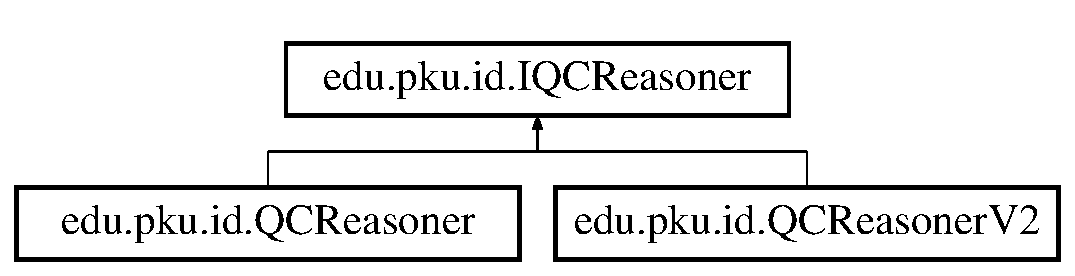
\includegraphics[height=2.000000cm]{interfaceedu_1_1pku_1_1id_1_1_i_q_c_reasoner}
\end{center}
\end{figure}
\subsection*{Public Member Functions}
\begin{DoxyCompactItemize}
\item 
abstract boolean \hyperlink{interfaceedu_1_1pku_1_1id_1_1_i_q_c_reasoner_a2cf3cc08877e6d06485e758bdbf5bf94}{qcEntails} (List$<$ IVecInt $>$ kb, IVecInt consequence)
\item 
abstract boolean \hyperlink{interfaceedu_1_1pku_1_1id_1_1_i_q_c_reasoner_a4d1172287213bd0be63dbd75f047aa7c}{isQcModel} (List$<$ IVecInt $>$ kb, List$<$ \hyperlink{namespaceedu_1_1pku_1_1id_a01cdd35063021f272bd905de5f43f634}{TruthValue} $>$ model)
\end{DoxyCompactItemize}


\subsection{Member Function Documentation}
\hypertarget{interfaceedu_1_1pku_1_1id_1_1_i_q_c_reasoner_a4d1172287213bd0be63dbd75f047aa7c}{
\index{edu::pku::id::IQCReasoner@{edu::pku::id::IQCReasoner}!isQcModel@{isQcModel}}
\index{isQcModel@{isQcModel}!edu::pku::id::IQCReasoner@{edu::pku::id::IQCReasoner}}
\subsubsection[{isQcModel}]{\setlength{\rightskip}{0pt plus 5cm}abstract boolean edu.pku.id.IQCReasoner.isQcModel (
\begin{DoxyParamCaption}
\item[{List$<$ IVecInt $>$}]{ kb, }
\item[{List$<$ {\bf TruthValue} $>$}]{ model}
\end{DoxyParamCaption}
)\hspace{0.3cm}{\ttfamily  \mbox{[}pure virtual\mbox{]}}}}
\label{interfaceedu_1_1pku_1_1id_1_1_i_q_c_reasoner_a4d1172287213bd0be63dbd75f047aa7c}


Implemented in \hyperlink{classedu_1_1pku_1_1id_1_1_q_c_reasoner_a98bdf18d6a8222310060877e6cff6d80}{edu.pku.id.QCReasoner}.

\hypertarget{interfaceedu_1_1pku_1_1id_1_1_i_q_c_reasoner_a2cf3cc08877e6d06485e758bdbf5bf94}{
\index{edu::pku::id::IQCReasoner@{edu::pku::id::IQCReasoner}!qcEntails@{qcEntails}}
\index{qcEntails@{qcEntails}!edu::pku::id::IQCReasoner@{edu::pku::id::IQCReasoner}}
\subsubsection[{qcEntails}]{\setlength{\rightskip}{0pt plus 5cm}abstract boolean edu.pku.id.IQCReasoner.qcEntails (
\begin{DoxyParamCaption}
\item[{List$<$ IVecInt $>$}]{ kb, }
\item[{IVecInt}]{ consequence}
\end{DoxyParamCaption}
)\hspace{0.3cm}{\ttfamily  \mbox{[}pure virtual\mbox{]}}}}
\label{interfaceedu_1_1pku_1_1id_1_1_i_q_c_reasoner_a2cf3cc08877e6d06485e758bdbf5bf94}
检测kb是否能够QC蕴含gamma


\begin{DoxyParams}{Parameters}
{\em kb} & 前提知识库,表示为子句的集合 \\
\hline
{\em consequence} & 结论,表示为子句 \\
\hline
\end{DoxyParams}
\begin{DoxyReturn}{Returns}
是否能够QC蕴含 
\end{DoxyReturn}


Implemented in \hyperlink{classedu_1_1pku_1_1id_1_1_q_c_reasoner_a0ce01daedfae2f88548978205d4848db}{edu.pku.id.QCReasoner}, and \hyperlink{classedu_1_1pku_1_1id_1_1_q_c_reasoner_v2_a04f22e9cef82ae44d46179d252ad46ef}{edu.pku.id.QCReasonerV2}.



The documentation for this interface was generated from the following file:\begin{DoxyCompactItemize}
\item 
src/edu/pku/id/\hyperlink{_i_q_c_reasoner_8java}{IQCReasoner.java}\end{DoxyCompactItemize}

\hypertarget{classgnu_1_1getopt_1_1_long_opt}{
\section{gnu.getopt.LongOpt Class Reference}
\label{classgnu_1_1getopt_1_1_long_opt}\index{gnu::getopt::LongOpt@{gnu::getopt::LongOpt}}
}
\subsection*{Public Member Functions}
\begin{DoxyCompactItemize}
\item 
\hyperlink{classgnu_1_1getopt_1_1_long_opt_a892ee836aff32542885ed3ddebb9d200}{LongOpt} (String \hyperlink{classgnu_1_1getopt_1_1_long_opt_a4b2a1686f77ce6aa2e36673cf0b074d9}{name}, int \hyperlink{classgnu_1_1getopt_1_1_long_opt_a7a8d529950461c0c30ef2df667df017b}{has\_\-arg}, StringBuffer \hyperlink{classgnu_1_1getopt_1_1_long_opt_ac9a762144573588ca158d909f65c03e9}{flag}, int \hyperlink{classgnu_1_1getopt_1_1_long_opt_aee56b4420df0cbd0f69788c7e4a3c57a}{val})  throws IllegalArgumentException 
\item 
String \hyperlink{classgnu_1_1getopt_1_1_long_opt_aaf2cc9e16562be40d61ee198095acb1c}{getName} ()
\item 
int \hyperlink{classgnu_1_1getopt_1_1_long_opt_a47d787d8b93010494fa587a7062328f0}{getHasArg} ()
\item 
StringBuffer \hyperlink{classgnu_1_1getopt_1_1_long_opt_ae10f9ea7c229f50fa58725d55c4e866f}{getFlag} ()
\item 
int \hyperlink{classgnu_1_1getopt_1_1_long_opt_ac03e7c48cc3baa3ca7bef7cddbc0fde7}{getVal} ()
\end{DoxyCompactItemize}
\subsection*{Static Public Attributes}
\begin{DoxyCompactItemize}
\item 
static final int \hyperlink{classgnu_1_1getopt_1_1_long_opt_a5af856e8de6a5f528d4da2b8706f7abe}{NO\_\-ARGUMENT} = 0
\item 
static final int \hyperlink{classgnu_1_1getopt_1_1_long_opt_a8105c98436b46a0b4de39a3afab230c2}{REQUIRED\_\-ARGUMENT} = 1
\item 
static final int \hyperlink{classgnu_1_1getopt_1_1_long_opt_a31819aae074fa1d80f547817640b31c1}{OPTIONAL\_\-ARGUMENT} = 2
\end{DoxyCompactItemize}
\subsection*{Protected Attributes}
\begin{DoxyCompactItemize}
\item 
String \hyperlink{classgnu_1_1getopt_1_1_long_opt_a4b2a1686f77ce6aa2e36673cf0b074d9}{name}
\item 
int \hyperlink{classgnu_1_1getopt_1_1_long_opt_a7a8d529950461c0c30ef2df667df017b}{has\_\-arg}
\item 
StringBuffer \hyperlink{classgnu_1_1getopt_1_1_long_opt_ac9a762144573588ca158d909f65c03e9}{flag}
\item 
int \hyperlink{classgnu_1_1getopt_1_1_long_opt_aee56b4420df0cbd0f69788c7e4a3c57a}{val}
\end{DoxyCompactItemize}
\subsection*{Private Attributes}
\begin{DoxyCompactItemize}
\item 
ResourceBundle \hyperlink{classgnu_1_1getopt_1_1_long_opt_af5966405b1f9dff812b8ee0641a4c13f}{\_\-messages}
\end{DoxyCompactItemize}


\subsection{Detailed Description}
This object represents the definition of a long option in the Java port of GNU getopt. An array of \hyperlink{classgnu_1_1getopt_1_1_long_opt}{LongOpt} objects is passed to the \hyperlink{classgnu_1_1getopt_1_1_getopt}{Getopt} object to define the list of valid long options for a given parsing session. Refer to the getopt documentation for details on the format of long options.

\begin{DoxyVersion}{Version}
1.0.5 
\end{DoxyVersion}
\begin{DoxyAuthor}{Author}
Aaron M. Renn (\href{mailto:arenn@urbanophile.com}{\tt arenn@urbanophile.com})
\end{DoxyAuthor}
\begin{DoxySeeAlso}{See also}
\hyperlink{classgnu_1_1getopt_1_1_getopt}{Getopt} 
\end{DoxySeeAlso}


\subsection{Constructor \& Destructor Documentation}
\hypertarget{classgnu_1_1getopt_1_1_long_opt_a892ee836aff32542885ed3ddebb9d200}{
\index{gnu::getopt::LongOpt@{gnu::getopt::LongOpt}!LongOpt@{LongOpt}}
\index{LongOpt@{LongOpt}!gnu::getopt::LongOpt@{gnu::getopt::LongOpt}}
\subsubsection[{LongOpt}]{\setlength{\rightskip}{0pt plus 5cm}gnu.getopt.LongOpt.LongOpt (
\begin{DoxyParamCaption}
\item[{String}]{ name, }
\item[{int}]{ has\_\-arg, }
\item[{StringBuffer}]{ flag, }
\item[{int}]{ val}
\end{DoxyParamCaption}
)  throws IllegalArgumentException }}
\label{classgnu_1_1getopt_1_1_long_opt_a892ee836aff32542885ed3ddebb9d200}
Create a new \hyperlink{classgnu_1_1getopt_1_1_long_opt}{LongOpt} object with the given parameter values. If the value passed as has\_\-arg is not valid, then an exception is thrown.


\begin{DoxyParams}{Parameters}
{\em name} & The long option String. \\
\hline
{\em has\_\-arg} & Indicates whether the option has no argument (NO\_\-ARGUMENT), a required argument (REQUIRED\_\-ARGUMENT) or an optional argument (OPTIONAL\_\-ARGUMENT). \\
\hline
{\em flag} & If non-\/null, this is a location to store the value of \char`\"{}val\char`\"{} when this option is encountered, otherwise \char`\"{}val\char`\"{} is treated as the equivalent short option character. \\
\hline
{\em val} & The value to return for this long option, or the equivalent single letter option to emulate if flag is null.\\
\hline
\end{DoxyParams}

\begin{DoxyExceptions}{Exceptions}
{\em IllegalArgumentException} & If the has\_\-arg param is not one of NO\_\-ARGUMENT, REQUIRED\_\-ARGUMENT or OPTIONAL\_\-ARGUMENT. \\
\hline
\end{DoxyExceptions}


\subsection{Member Function Documentation}
\hypertarget{classgnu_1_1getopt_1_1_long_opt_ae10f9ea7c229f50fa58725d55c4e866f}{
\index{gnu::getopt::LongOpt@{gnu::getopt::LongOpt}!getFlag@{getFlag}}
\index{getFlag@{getFlag}!gnu::getopt::LongOpt@{gnu::getopt::LongOpt}}
\subsubsection[{getFlag}]{\setlength{\rightskip}{0pt plus 5cm}StringBuffer gnu.getopt.LongOpt.getFlag (
\begin{DoxyParamCaption}
{}
\end{DoxyParamCaption}
)}}
\label{classgnu_1_1getopt_1_1_long_opt_ae10f9ea7c229f50fa58725d55c4e866f}
Returns the value of the 'flag' field for this long option

\begin{DoxyReturn}{Returns}
The value of 'flag' 
\end{DoxyReturn}
\hypertarget{classgnu_1_1getopt_1_1_long_opt_a47d787d8b93010494fa587a7062328f0}{
\index{gnu::getopt::LongOpt@{gnu::getopt::LongOpt}!getHasArg@{getHasArg}}
\index{getHasArg@{getHasArg}!gnu::getopt::LongOpt@{gnu::getopt::LongOpt}}
\subsubsection[{getHasArg}]{\setlength{\rightskip}{0pt plus 5cm}int gnu.getopt.LongOpt.getHasArg (
\begin{DoxyParamCaption}
{}
\end{DoxyParamCaption}
)}}
\label{classgnu_1_1getopt_1_1_long_opt_a47d787d8b93010494fa587a7062328f0}
Returns the value set for the 'has\_\-arg' field for this long option

\begin{DoxyReturn}{Returns}
The value of 'has\_\-arg' 
\end{DoxyReturn}
\hypertarget{classgnu_1_1getopt_1_1_long_opt_aaf2cc9e16562be40d61ee198095acb1c}{
\index{gnu::getopt::LongOpt@{gnu::getopt::LongOpt}!getName@{getName}}
\index{getName@{getName}!gnu::getopt::LongOpt@{gnu::getopt::LongOpt}}
\subsubsection[{getName}]{\setlength{\rightskip}{0pt plus 5cm}String gnu.getopt.LongOpt.getName (
\begin{DoxyParamCaption}
{}
\end{DoxyParamCaption}
)}}
\label{classgnu_1_1getopt_1_1_long_opt_aaf2cc9e16562be40d61ee198095acb1c}
Returns the name of this \hyperlink{classgnu_1_1getopt_1_1_long_opt}{LongOpt} as a String

\begin{DoxyReturn}{Returns}
Then name of the long option 
\end{DoxyReturn}
\hypertarget{classgnu_1_1getopt_1_1_long_opt_ac03e7c48cc3baa3ca7bef7cddbc0fde7}{
\index{gnu::getopt::LongOpt@{gnu::getopt::LongOpt}!getVal@{getVal}}
\index{getVal@{getVal}!gnu::getopt::LongOpt@{gnu::getopt::LongOpt}}
\subsubsection[{getVal}]{\setlength{\rightskip}{0pt plus 5cm}int gnu.getopt.LongOpt.getVal (
\begin{DoxyParamCaption}
{}
\end{DoxyParamCaption}
)}}
\label{classgnu_1_1getopt_1_1_long_opt_ac03e7c48cc3baa3ca7bef7cddbc0fde7}
Returns the value of the 'val' field for this long option

\begin{DoxyReturn}{Returns}
The value of 'val' 
\end{DoxyReturn}


\subsection{Member Data Documentation}
\hypertarget{classgnu_1_1getopt_1_1_long_opt_af5966405b1f9dff812b8ee0641a4c13f}{
\index{gnu::getopt::LongOpt@{gnu::getopt::LongOpt}!\_\-messages@{\_\-messages}}
\index{\_\-messages@{\_\-messages}!gnu::getopt::LongOpt@{gnu::getopt::LongOpt}}
\subsubsection[{\_\-messages}]{\setlength{\rightskip}{0pt plus 5cm}ResourceBundle {\bf gnu.getopt.LongOpt.\_\-messages}\hspace{0.3cm}{\ttfamily  \mbox{[}private\mbox{]}}}}
\label{classgnu_1_1getopt_1_1_long_opt_af5966405b1f9dff812b8ee0641a4c13f}
{\bfseries Initial value:}
\begin{DoxyCode}
 PropertyResourceBundle.getBundle(
                            "gnu/getopt/MessagesBundle", Locale.getDefault())
\end{DoxyCode}
Localized strings for error messages \hypertarget{classgnu_1_1getopt_1_1_long_opt_ac9a762144573588ca158d909f65c03e9}{
\index{gnu::getopt::LongOpt@{gnu::getopt::LongOpt}!flag@{flag}}
\index{flag@{flag}!gnu::getopt::LongOpt@{gnu::getopt::LongOpt}}
\subsubsection[{flag}]{\setlength{\rightskip}{0pt plus 5cm}StringBuffer {\bf gnu.getopt.LongOpt.flag}\hspace{0.3cm}{\ttfamily  \mbox{[}protected\mbox{]}}}}
\label{classgnu_1_1getopt_1_1_long_opt_ac9a762144573588ca158d909f65c03e9}
If this variable is not null, then the value stored in \char`\"{}val\char`\"{} is stored here when this long option is encountered. If this is null, the value stored in \char`\"{}val\char`\"{} is treated as the name of an equivalent short option. \hypertarget{classgnu_1_1getopt_1_1_long_opt_a7a8d529950461c0c30ef2df667df017b}{
\index{gnu::getopt::LongOpt@{gnu::getopt::LongOpt}!has\_\-arg@{has\_\-arg}}
\index{has\_\-arg@{has\_\-arg}!gnu::getopt::LongOpt@{gnu::getopt::LongOpt}}
\subsubsection[{has\_\-arg}]{\setlength{\rightskip}{0pt plus 5cm}int {\bf gnu.getopt.LongOpt.has\_\-arg}\hspace{0.3cm}{\ttfamily  \mbox{[}protected\mbox{]}}}}
\label{classgnu_1_1getopt_1_1_long_opt_a7a8d529950461c0c30ef2df667df017b}
Indicates whether the option has no argument, a required argument, or an optional argument. \hypertarget{classgnu_1_1getopt_1_1_long_opt_a4b2a1686f77ce6aa2e36673cf0b074d9}{
\index{gnu::getopt::LongOpt@{gnu::getopt::LongOpt}!name@{name}}
\index{name@{name}!gnu::getopt::LongOpt@{gnu::getopt::LongOpt}}
\subsubsection[{name}]{\setlength{\rightskip}{0pt plus 5cm}String {\bf gnu.getopt.LongOpt.name}\hspace{0.3cm}{\ttfamily  \mbox{[}protected\mbox{]}}}}
\label{classgnu_1_1getopt_1_1_long_opt_a4b2a1686f77ce6aa2e36673cf0b074d9}
The name of the long option \hypertarget{classgnu_1_1getopt_1_1_long_opt_a5af856e8de6a5f528d4da2b8706f7abe}{
\index{gnu::getopt::LongOpt@{gnu::getopt::LongOpt}!NO\_\-ARGUMENT@{NO\_\-ARGUMENT}}
\index{NO\_\-ARGUMENT@{NO\_\-ARGUMENT}!gnu::getopt::LongOpt@{gnu::getopt::LongOpt}}
\subsubsection[{NO\_\-ARGUMENT}]{\setlength{\rightskip}{0pt plus 5cm}final int {\bf gnu.getopt.LongOpt.NO\_\-ARGUMENT} = 0\hspace{0.3cm}{\ttfamily  \mbox{[}static\mbox{]}}}}
\label{classgnu_1_1getopt_1_1_long_opt_a5af856e8de6a5f528d4da2b8706f7abe}
Constant value used for the \char`\"{}has\_\-arg\char`\"{} constructor argument. This value indicates that the option takes no argument. \hypertarget{classgnu_1_1getopt_1_1_long_opt_a31819aae074fa1d80f547817640b31c1}{
\index{gnu::getopt::LongOpt@{gnu::getopt::LongOpt}!OPTIONAL\_\-ARGUMENT@{OPTIONAL\_\-ARGUMENT}}
\index{OPTIONAL\_\-ARGUMENT@{OPTIONAL\_\-ARGUMENT}!gnu::getopt::LongOpt@{gnu::getopt::LongOpt}}
\subsubsection[{OPTIONAL\_\-ARGUMENT}]{\setlength{\rightskip}{0pt plus 5cm}final int {\bf gnu.getopt.LongOpt.OPTIONAL\_\-ARGUMENT} = 2\hspace{0.3cm}{\ttfamily  \mbox{[}static\mbox{]}}}}
\label{classgnu_1_1getopt_1_1_long_opt_a31819aae074fa1d80f547817640b31c1}
Constant value used for the \char`\"{}has\_\-arg\char`\"{} constructor argument. This value indicates that the option takes an argument that is optional. \hypertarget{classgnu_1_1getopt_1_1_long_opt_a8105c98436b46a0b4de39a3afab230c2}{
\index{gnu::getopt::LongOpt@{gnu::getopt::LongOpt}!REQUIRED\_\-ARGUMENT@{REQUIRED\_\-ARGUMENT}}
\index{REQUIRED\_\-ARGUMENT@{REQUIRED\_\-ARGUMENT}!gnu::getopt::LongOpt@{gnu::getopt::LongOpt}}
\subsubsection[{REQUIRED\_\-ARGUMENT}]{\setlength{\rightskip}{0pt plus 5cm}final int {\bf gnu.getopt.LongOpt.REQUIRED\_\-ARGUMENT} = 1\hspace{0.3cm}{\ttfamily  \mbox{[}static\mbox{]}}}}
\label{classgnu_1_1getopt_1_1_long_opt_a8105c98436b46a0b4de39a3afab230c2}
Constant value used for the \char`\"{}has\_\-arg\char`\"{} constructor argument. This value indicates that the option takes an argument that is required. \hypertarget{classgnu_1_1getopt_1_1_long_opt_aee56b4420df0cbd0f69788c7e4a3c57a}{
\index{gnu::getopt::LongOpt@{gnu::getopt::LongOpt}!val@{val}}
\index{val@{val}!gnu::getopt::LongOpt@{gnu::getopt::LongOpt}}
\subsubsection[{val}]{\setlength{\rightskip}{0pt plus 5cm}int {\bf gnu.getopt.LongOpt.val}\hspace{0.3cm}{\ttfamily  \mbox{[}protected\mbox{]}}}}
\label{classgnu_1_1getopt_1_1_long_opt_aee56b4420df0cbd0f69788c7e4a3c57a}
The value to store in \char`\"{}flag\char`\"{} if flag is not null, otherwise the equivalent short option character for this long option. 

The documentation for this class was generated from the following file:\begin{DoxyCompactItemize}
\item 
src/gnu/getopt/\hyperlink{_long_opt_8java}{LongOpt.java}\end{DoxyCompactItemize}

\hypertarget{classedu_1_1pku_1_1id_1_1_multi_valued_translater}{
\section{edu.pku.id.MultiValuedTranslater Class Reference}
\label{classedu_1_1pku_1_1id_1_1_multi_valued_translater}\index{edu::pku::id::MultiValuedTranslater@{edu::pku::id::MultiValuedTranslater}}
}
Inheritance diagram for edu.pku.id.MultiValuedTranslater:\begin{figure}[H]
\begin{center}
\leavevmode
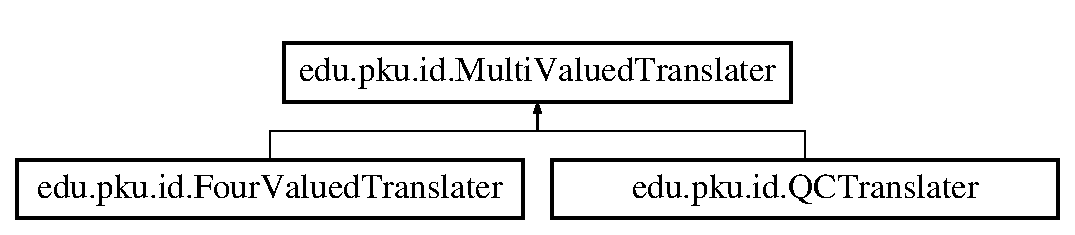
\includegraphics[height=2.000000cm]{classedu_1_1pku_1_1id_1_1_multi_valued_translater}
\end{center}
\end{figure}
\subsection*{Public Member Functions}
\begin{DoxyCompactItemize}
\item 
void \hyperlink{classedu_1_1pku_1_1id_1_1_multi_valued_translater_a04258517c65ce4b3463294ea4c78b74b}{countVars} ()
\item 
List$<$ \hyperlink{classedu_1_1pku_1_1id_1_1_weighted_clause}{WeightedClause} $>$ \hyperlink{classedu_1_1pku_1_1id_1_1_multi_valued_translater_ac5c20fd88b29e9df2837e711bf236c11}{getWeightedClauses} ()
\item 
void \hyperlink{classedu_1_1pku_1_1id_1_1_multi_valued_translater_a5f20e760fdc78e31ea00770274b0b3a6}{setClauses} (List$<$ IVecInt $>$ \hyperlink{classedu_1_1pku_1_1id_1_1_multi_valued_translater_ac5e73cd4928c489b13949689250bdd33}{clauses})
\item 
int \hyperlink{classedu_1_1pku_1_1id_1_1_multi_valued_translater_ae2bc7bb42344c252fa310e0a27928fb8}{getNVars} ()
\end{DoxyCompactItemize}
\subsection*{Static Public Member Functions}
\begin{DoxyCompactItemize}
\item 
static \hyperlink{classedu_1_1pku_1_1id_1_1_multi_valued_translater}{MultiValuedTranslater} \hyperlink{classedu_1_1pku_1_1id_1_1_multi_valued_translater_a966c7a4cf64060a6417f811eba77775d}{create} (\hyperlink{namespaceedu_1_1pku_1_1id_ad71ddcb0be4b31cdeeb2a5d755309f2d}{MultiValuedSemantics} semantics)
\end{DoxyCompactItemize}
\subsection*{Protected Member Functions}
\begin{DoxyCompactItemize}
\item 
int \hyperlink{classedu_1_1pku_1_1id_1_1_multi_valued_translater_a4d45510950867b77da6a77692a57abb2}{translateLiteral} (int literal)
\end{DoxyCompactItemize}
\subsection*{Package Functions}
\begin{DoxyCompactItemize}
\item 
abstract void \hyperlink{classedu_1_1pku_1_1id_1_1_multi_valued_translater_a57e687a8b1c011fb7c0ccbd72272e328}{translate} ()
\end{DoxyCompactItemize}
\subsection*{Package Attributes}
\begin{DoxyCompactItemize}
\item 
int \hyperlink{classedu_1_1pku_1_1id_1_1_multi_valued_translater_ac32ccbcc28ed991632d9d95eeb10f279}{nVars} = 0
\item 
List$<$ IVecInt $>$ \hyperlink{classedu_1_1pku_1_1id_1_1_multi_valued_translater_ac5e73cd4928c489b13949689250bdd33}{clauses}
\item 
List$<$ \hyperlink{classedu_1_1pku_1_1id_1_1_weighted_clause}{WeightedClause} $>$ \hyperlink{classedu_1_1pku_1_1id_1_1_multi_valued_translater_af8448dcc0a0420748f9d331c0be01ef2}{weightedClauses}
\item 
boolean \hyperlink{classedu_1_1pku_1_1id_1_1_multi_valued_translater_a201fef561c0cfbcd87bae63db0ec4c1a}{translated} = false
\end{DoxyCompactItemize}


\subsection{Member Function Documentation}
\hypertarget{classedu_1_1pku_1_1id_1_1_multi_valued_translater_a04258517c65ce4b3463294ea4c78b74b}{
\index{edu::pku::id::MultiValuedTranslater@{edu::pku::id::MultiValuedTranslater}!countVars@{countVars}}
\index{countVars@{countVars}!edu::pku::id::MultiValuedTranslater@{edu::pku::id::MultiValuedTranslater}}
\subsubsection[{countVars}]{\setlength{\rightskip}{0pt plus 5cm}void edu.pku.id.MultiValuedTranslater.countVars (
\begin{DoxyParamCaption}
{}
\end{DoxyParamCaption}
)}}
\label{classedu_1_1pku_1_1id_1_1_multi_valued_translater_a04258517c65ce4b3463294ea4c78b74b}
\hypertarget{classedu_1_1pku_1_1id_1_1_multi_valued_translater_a966c7a4cf64060a6417f811eba77775d}{
\index{edu::pku::id::MultiValuedTranslater@{edu::pku::id::MultiValuedTranslater}!create@{create}}
\index{create@{create}!edu::pku::id::MultiValuedTranslater@{edu::pku::id::MultiValuedTranslater}}
\subsubsection[{create}]{\setlength{\rightskip}{0pt plus 5cm}static {\bf MultiValuedTranslater} edu.pku.id.MultiValuedTranslater.create (
\begin{DoxyParamCaption}
\item[{{\bf MultiValuedSemantics}}]{ semantics}
\end{DoxyParamCaption}
)\hspace{0.3cm}{\ttfamily  \mbox{[}static\mbox{]}}}}
\label{classedu_1_1pku_1_1id_1_1_multi_valued_translater_a966c7a4cf64060a6417f811eba77775d}
\hypertarget{classedu_1_1pku_1_1id_1_1_multi_valued_translater_ae2bc7bb42344c252fa310e0a27928fb8}{
\index{edu::pku::id::MultiValuedTranslater@{edu::pku::id::MultiValuedTranslater}!getNVars@{getNVars}}
\index{getNVars@{getNVars}!edu::pku::id::MultiValuedTranslater@{edu::pku::id::MultiValuedTranslater}}
\subsubsection[{getNVars}]{\setlength{\rightskip}{0pt plus 5cm}int edu.pku.id.MultiValuedTranslater.getNVars (
\begin{DoxyParamCaption}
{}
\end{DoxyParamCaption}
)}}
\label{classedu_1_1pku_1_1id_1_1_multi_valued_translater_ae2bc7bb42344c252fa310e0a27928fb8}
\hypertarget{classedu_1_1pku_1_1id_1_1_multi_valued_translater_ac5c20fd88b29e9df2837e711bf236c11}{
\index{edu::pku::id::MultiValuedTranslater@{edu::pku::id::MultiValuedTranslater}!getWeightedClauses@{getWeightedClauses}}
\index{getWeightedClauses@{getWeightedClauses}!edu::pku::id::MultiValuedTranslater@{edu::pku::id::MultiValuedTranslater}}
\subsubsection[{getWeightedClauses}]{\setlength{\rightskip}{0pt plus 5cm}List$<${\bf WeightedClause}$>$ edu.pku.id.MultiValuedTranslater.getWeightedClauses (
\begin{DoxyParamCaption}
{}
\end{DoxyParamCaption}
)}}
\label{classedu_1_1pku_1_1id_1_1_multi_valued_translater_ac5c20fd88b29e9df2837e711bf236c11}
\hypertarget{classedu_1_1pku_1_1id_1_1_multi_valued_translater_a5f20e760fdc78e31ea00770274b0b3a6}{
\index{edu::pku::id::MultiValuedTranslater@{edu::pku::id::MultiValuedTranslater}!setClauses@{setClauses}}
\index{setClauses@{setClauses}!edu::pku::id::MultiValuedTranslater@{edu::pku::id::MultiValuedTranslater}}
\subsubsection[{setClauses}]{\setlength{\rightskip}{0pt plus 5cm}void edu.pku.id.MultiValuedTranslater.setClauses (
\begin{DoxyParamCaption}
\item[{List$<$ IVecInt $>$}]{ clauses}
\end{DoxyParamCaption}
)}}
\label{classedu_1_1pku_1_1id_1_1_multi_valued_translater_a5f20e760fdc78e31ea00770274b0b3a6}
\hypertarget{classedu_1_1pku_1_1id_1_1_multi_valued_translater_a57e687a8b1c011fb7c0ccbd72272e328}{
\index{edu::pku::id::MultiValuedTranslater@{edu::pku::id::MultiValuedTranslater}!translate@{translate}}
\index{translate@{translate}!edu::pku::id::MultiValuedTranslater@{edu::pku::id::MultiValuedTranslater}}
\subsubsection[{translate}]{\setlength{\rightskip}{0pt plus 5cm}abstract void edu.pku.id.MultiValuedTranslater.translate (
\begin{DoxyParamCaption}
{}
\end{DoxyParamCaption}
)\hspace{0.3cm}{\ttfamily  \mbox{[}package, pure virtual\mbox{]}}}}
\label{classedu_1_1pku_1_1id_1_1_multi_valued_translater_a57e687a8b1c011fb7c0ccbd72272e328}


Implemented in \hyperlink{classedu_1_1pku_1_1id_1_1_four_valued_translater_a364637e20334ca6017ceffb49de3e551}{edu.pku.id.FourValuedTranslater}, and \hyperlink{classedu_1_1pku_1_1id_1_1_q_c_translater_a2b3b851d0bcb6cbfc07badd6e6434096}{edu.pku.id.QCTranslater}.

\hypertarget{classedu_1_1pku_1_1id_1_1_multi_valued_translater_a4d45510950867b77da6a77692a57abb2}{
\index{edu::pku::id::MultiValuedTranslater@{edu::pku::id::MultiValuedTranslater}!translateLiteral@{translateLiteral}}
\index{translateLiteral@{translateLiteral}!edu::pku::id::MultiValuedTranslater@{edu::pku::id::MultiValuedTranslater}}
\subsubsection[{translateLiteral}]{\setlength{\rightskip}{0pt plus 5cm}int edu.pku.id.MultiValuedTranslater.translateLiteral (
\begin{DoxyParamCaption}
\item[{int}]{ literal}
\end{DoxyParamCaption}
)\hspace{0.3cm}{\ttfamily  \mbox{[}protected\mbox{]}}}}
\label{classedu_1_1pku_1_1id_1_1_multi_valued_translater_a4d45510950867b77da6a77692a57abb2}


\subsection{Member Data Documentation}
\hypertarget{classedu_1_1pku_1_1id_1_1_multi_valued_translater_ac5e73cd4928c489b13949689250bdd33}{
\index{edu::pku::id::MultiValuedTranslater@{edu::pku::id::MultiValuedTranslater}!clauses@{clauses}}
\index{clauses@{clauses}!edu::pku::id::MultiValuedTranslater@{edu::pku::id::MultiValuedTranslater}}
\subsubsection[{clauses}]{\setlength{\rightskip}{0pt plus 5cm}List$<$IVecInt$>$ {\bf edu.pku.id.MultiValuedTranslater.clauses}\hspace{0.3cm}{\ttfamily  \mbox{[}package\mbox{]}}}}
\label{classedu_1_1pku_1_1id_1_1_multi_valued_translater_ac5e73cd4928c489b13949689250bdd33}
\hypertarget{classedu_1_1pku_1_1id_1_1_multi_valued_translater_ac32ccbcc28ed991632d9d95eeb10f279}{
\index{edu::pku::id::MultiValuedTranslater@{edu::pku::id::MultiValuedTranslater}!nVars@{nVars}}
\index{nVars@{nVars}!edu::pku::id::MultiValuedTranslater@{edu::pku::id::MultiValuedTranslater}}
\subsubsection[{nVars}]{\setlength{\rightskip}{0pt plus 5cm}int {\bf edu.pku.id.MultiValuedTranslater.nVars} = 0\hspace{0.3cm}{\ttfamily  \mbox{[}package\mbox{]}}}}
\label{classedu_1_1pku_1_1id_1_1_multi_valued_translater_ac32ccbcc28ed991632d9d95eeb10f279}
\hypertarget{classedu_1_1pku_1_1id_1_1_multi_valued_translater_a201fef561c0cfbcd87bae63db0ec4c1a}{
\index{edu::pku::id::MultiValuedTranslater@{edu::pku::id::MultiValuedTranslater}!translated@{translated}}
\index{translated@{translated}!edu::pku::id::MultiValuedTranslater@{edu::pku::id::MultiValuedTranslater}}
\subsubsection[{translated}]{\setlength{\rightskip}{0pt plus 5cm}boolean {\bf edu.pku.id.MultiValuedTranslater.translated} = false\hspace{0.3cm}{\ttfamily  \mbox{[}package\mbox{]}}}}
\label{classedu_1_1pku_1_1id_1_1_multi_valued_translater_a201fef561c0cfbcd87bae63db0ec4c1a}
\hypertarget{classedu_1_1pku_1_1id_1_1_multi_valued_translater_af8448dcc0a0420748f9d331c0be01ef2}{
\index{edu::pku::id::MultiValuedTranslater@{edu::pku::id::MultiValuedTranslater}!weightedClauses@{weightedClauses}}
\index{weightedClauses@{weightedClauses}!edu::pku::id::MultiValuedTranslater@{edu::pku::id::MultiValuedTranslater}}
\subsubsection[{weightedClauses}]{\setlength{\rightskip}{0pt plus 5cm}List$<${\bf WeightedClause}$>$ {\bf edu.pku.id.MultiValuedTranslater.weightedClauses}\hspace{0.3cm}{\ttfamily  \mbox{[}package\mbox{]}}}}
\label{classedu_1_1pku_1_1id_1_1_multi_valued_translater_af8448dcc0a0420748f9d331c0be01ef2}


The documentation for this class was generated from the following file:\begin{DoxyCompactItemize}
\item 
src/edu/pku/id/\hyperlink{_multi_valued_translater_8java}{MultiValuedTranslater.java}\end{DoxyCompactItemize}

\hypertarget{classedu_1_1pku_1_1id_1_1cli_1_1_multi_valued_translater_cli}{
\section{edu.pku.id.cli.MultiValuedTranslaterCli Class Reference}
\label{classedu_1_1pku_1_1id_1_1cli_1_1_multi_valued_translater_cli}\index{edu::pku::id::cli::MultiValuedTranslaterCli@{edu::pku::id::cli::MultiValuedTranslaterCli}}
}
\subsection*{Static Public Member Functions}
\begin{DoxyCompactItemize}
\item 
static void \hyperlink{classedu_1_1pku_1_1id_1_1cli_1_1_multi_valued_translater_cli_a1497d0ce5a0281ae2feed043416cd002}{main} (String\mbox{[}$\,$\mbox{]} argv)  throws IOException, ParseFormatException 
\end{DoxyCompactItemize}


\subsection{Member Function Documentation}
\hypertarget{classedu_1_1pku_1_1id_1_1cli_1_1_multi_valued_translater_cli_a1497d0ce5a0281ae2feed043416cd002}{
\index{edu::pku::id::cli::MultiValuedTranslaterCli@{edu::pku::id::cli::MultiValuedTranslaterCli}!main@{main}}
\index{main@{main}!edu::pku::id::cli::MultiValuedTranslaterCli@{edu::pku::id::cli::MultiValuedTranslaterCli}}
\subsubsection[{main}]{\setlength{\rightskip}{0pt plus 5cm}static void edu.pku.id.cli.MultiValuedTranslaterCli.main (
\begin{DoxyParamCaption}
\item[{String\mbox{[}$\,$\mbox{]}}]{ argv}
\end{DoxyParamCaption}
)  throws IOException, ParseFormatException \hspace{0.3cm}{\ttfamily  \mbox{[}static\mbox{]}}}}
\label{classedu_1_1pku_1_1id_1_1cli_1_1_multi_valued_translater_cli_a1497d0ce5a0281ae2feed043416cd002}

\begin{DoxyParams}{Parameters}
{\em args} & \\
\hline
\end{DoxyParams}

\begin{DoxyExceptions}{Exceptions}
{\em ParseFormatException} & \\
\hline
{\em IOException} & \\
\hline
\end{DoxyExceptions}


The documentation for this class was generated from the following file:\begin{DoxyCompactItemize}
\item 
src/edu/pku/id/cli/\hyperlink{_multi_valued_translater_cli_8java}{MultiValuedTranslaterCli.java}\end{DoxyCompactItemize}

\hypertarget{classedu_1_1pku_1_1id_1_1file_1_1_m_u_s_file_reader}{
\section{edu.pku.id.file.MUSFileReader Class Reference}
\label{classedu_1_1pku_1_1id_1_1file_1_1_m_u_s_file_reader}\index{edu::pku::id::file::MUSFileReader@{edu::pku::id::file::MUSFileReader}}
}
\subsection*{Public Member Functions}
\begin{DoxyCompactItemize}
\item 
\hyperlink{classedu_1_1pku_1_1id_1_1file_1_1_m_u_s_file_reader_aa37746001f3fb55704ea6f275dbfa9b2}{MUSFileReader} (String fileName)  throws FileNotFoundException 
\item 
\hyperlink{classedu_1_1pku_1_1id_1_1file_1_1_m_u_s_file_reader_a753bff7f7238d13211abfa17c531741a}{MUSFileReader} (LineNumberReader reader)
\item 
List$<$ List$<$ Integer $>$ $>$ \hyperlink{classedu_1_1pku_1_1id_1_1file_1_1_m_u_s_file_reader_a8367a47506baf8841ffb88aa4180d31d}{read} ()  throws IOException 
\end{DoxyCompactItemize}
\subsection*{Private Attributes}
\begin{DoxyCompactItemize}
\item 
LineNumberReader \hyperlink{classedu_1_1pku_1_1id_1_1file_1_1_m_u_s_file_reader_af176cb943376789226dd691f24f6c2e6}{in}
\item 
List$<$ List$<$ Integer $>$ $>$ \hyperlink{classedu_1_1pku_1_1id_1_1file_1_1_m_u_s_file_reader_ae7598813fc97a674c9dfdc50f79f1d52}{muses}
\end{DoxyCompactItemize}


\subsection{Constructor \& Destructor Documentation}
\hypertarget{classedu_1_1pku_1_1id_1_1file_1_1_m_u_s_file_reader_aa37746001f3fb55704ea6f275dbfa9b2}{
\index{edu::pku::id::file::MUSFileReader@{edu::pku::id::file::MUSFileReader}!MUSFileReader@{MUSFileReader}}
\index{MUSFileReader@{MUSFileReader}!edu::pku::id::file::MUSFileReader@{edu::pku::id::file::MUSFileReader}}
\subsubsection[{MUSFileReader}]{\setlength{\rightskip}{0pt plus 5cm}edu.pku.id.file.MUSFileReader.MUSFileReader (
\begin{DoxyParamCaption}
\item[{String}]{ fileName}
\end{DoxyParamCaption}
)  throws FileNotFoundException }}
\label{classedu_1_1pku_1_1id_1_1file_1_1_m_u_s_file_reader_aa37746001f3fb55704ea6f275dbfa9b2}
\hypertarget{classedu_1_1pku_1_1id_1_1file_1_1_m_u_s_file_reader_a753bff7f7238d13211abfa17c531741a}{
\index{edu::pku::id::file::MUSFileReader@{edu::pku::id::file::MUSFileReader}!MUSFileReader@{MUSFileReader}}
\index{MUSFileReader@{MUSFileReader}!edu::pku::id::file::MUSFileReader@{edu::pku::id::file::MUSFileReader}}
\subsubsection[{MUSFileReader}]{\setlength{\rightskip}{0pt plus 5cm}edu.pku.id.file.MUSFileReader.MUSFileReader (
\begin{DoxyParamCaption}
\item[{LineNumberReader}]{ reader}
\end{DoxyParamCaption}
)}}
\label{classedu_1_1pku_1_1id_1_1file_1_1_m_u_s_file_reader_a753bff7f7238d13211abfa17c531741a}


\subsection{Member Function Documentation}
\hypertarget{classedu_1_1pku_1_1id_1_1file_1_1_m_u_s_file_reader_a8367a47506baf8841ffb88aa4180d31d}{
\index{edu::pku::id::file::MUSFileReader@{edu::pku::id::file::MUSFileReader}!read@{read}}
\index{read@{read}!edu::pku::id::file::MUSFileReader@{edu::pku::id::file::MUSFileReader}}
\subsubsection[{read}]{\setlength{\rightskip}{0pt plus 5cm}List$<$List$<$Integer$>$ $>$ edu.pku.id.file.MUSFileReader.read (
\begin{DoxyParamCaption}
{}
\end{DoxyParamCaption}
)  throws IOException }}
\label{classedu_1_1pku_1_1id_1_1file_1_1_m_u_s_file_reader_a8367a47506baf8841ffb88aa4180d31d}


\subsection{Member Data Documentation}
\hypertarget{classedu_1_1pku_1_1id_1_1file_1_1_m_u_s_file_reader_af176cb943376789226dd691f24f6c2e6}{
\index{edu::pku::id::file::MUSFileReader@{edu::pku::id::file::MUSFileReader}!in@{in}}
\index{in@{in}!edu::pku::id::file::MUSFileReader@{edu::pku::id::file::MUSFileReader}}
\subsubsection[{in}]{\setlength{\rightskip}{0pt plus 5cm}LineNumberReader {\bf edu.pku.id.file.MUSFileReader.in}\hspace{0.3cm}{\ttfamily  \mbox{[}private\mbox{]}}}}
\label{classedu_1_1pku_1_1id_1_1file_1_1_m_u_s_file_reader_af176cb943376789226dd691f24f6c2e6}
\hypertarget{classedu_1_1pku_1_1id_1_1file_1_1_m_u_s_file_reader_ae7598813fc97a674c9dfdc50f79f1d52}{
\index{edu::pku::id::file::MUSFileReader@{edu::pku::id::file::MUSFileReader}!muses@{muses}}
\index{muses@{muses}!edu::pku::id::file::MUSFileReader@{edu::pku::id::file::MUSFileReader}}
\subsubsection[{muses}]{\setlength{\rightskip}{0pt plus 5cm}List$<$List$<$Integer$>$ $>$ {\bf edu.pku.id.file.MUSFileReader.muses}\hspace{0.3cm}{\ttfamily  \mbox{[}private\mbox{]}}}}
\label{classedu_1_1pku_1_1id_1_1file_1_1_m_u_s_file_reader_ae7598813fc97a674c9dfdc50f79f1d52}


The documentation for this class was generated from the following file:\begin{DoxyCompactItemize}
\item 
src/edu/pku/id/file/\hyperlink{_m_u_s_file_reader_8java}{MUSFileReader.java}\end{DoxyCompactItemize}

\hypertarget{classedu_1_1pku_1_1id_1_1_partial_max_s_a_t_writer}{
\section{edu.pku.id.PartialMaxSATWriter Class Reference}
\label{classedu_1_1pku_1_1id_1_1_partial_max_s_a_t_writer}\index{edu::pku::id::PartialMaxSATWriter@{edu::pku::id::PartialMaxSATWriter}}
}
Inheritance diagram for edu.pku.id.PartialMaxSATWriter:\begin{figure}[H]
\begin{center}
\leavevmode
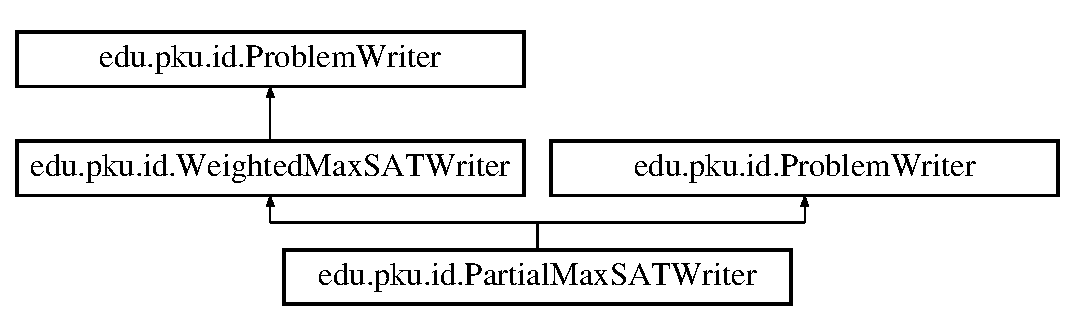
\includegraphics[height=3.000000cm]{classedu_1_1pku_1_1id_1_1_partial_max_s_a_t_writer}
\end{center}
\end{figure}
\subsection*{Public Member Functions}
\begin{DoxyCompactItemize}
\item 
\hyperlink{classedu_1_1pku_1_1id_1_1_partial_max_s_a_t_writer_a59072d3e1439a0bf31b35aedb1cfffc3}{PartialMaxSATWriter} (List$<$ \hyperlink{classedu_1_1pku_1_1id_1_1_weighted_clause}{WeightedClause} $>$ \hyperlink{classedu_1_1pku_1_1id_1_1_weighted_max_s_a_t_writer_a73dc99c36bfbaf938f3ffb7b95189d37}{weightedClauses}, int \hyperlink{classedu_1_1pku_1_1id_1_1_weighted_max_s_a_t_writer_ae9c3e5d651a1b8100fd5d85f00a18a54}{nbVars}, String fileName)  throws IOException 
\end{DoxyCompactItemize}
\subsection*{Protected Member Functions}
\begin{DoxyCompactItemize}
\item 
void \hyperlink{classedu_1_1pku_1_1id_1_1_partial_max_s_a_t_writer_ab066f4e7f38654fefdeb3cc02b56026f}{writeProblem} ()  throws IOException 
\end{DoxyCompactItemize}


\subsection{Constructor \& Destructor Documentation}
\hypertarget{classedu_1_1pku_1_1id_1_1_partial_max_s_a_t_writer_a59072d3e1439a0bf31b35aedb1cfffc3}{
\index{edu::pku::id::PartialMaxSATWriter@{edu::pku::id::PartialMaxSATWriter}!PartialMaxSATWriter@{PartialMaxSATWriter}}
\index{PartialMaxSATWriter@{PartialMaxSATWriter}!edu::pku::id::PartialMaxSATWriter@{edu::pku::id::PartialMaxSATWriter}}
\subsubsection[{PartialMaxSATWriter}]{\setlength{\rightskip}{0pt plus 5cm}edu.pku.id.PartialMaxSATWriter.PartialMaxSATWriter (
\begin{DoxyParamCaption}
\item[{List$<$ {\bf WeightedClause} $>$}]{ weightedClauses, }
\item[{int}]{ nbVars, }
\item[{String}]{ fileName}
\end{DoxyParamCaption}
)  throws IOException }}
\label{classedu_1_1pku_1_1id_1_1_partial_max_s_a_t_writer_a59072d3e1439a0bf31b35aedb1cfffc3}


\subsection{Member Function Documentation}
\hypertarget{classedu_1_1pku_1_1id_1_1_partial_max_s_a_t_writer_ab066f4e7f38654fefdeb3cc02b56026f}{
\index{edu::pku::id::PartialMaxSATWriter@{edu::pku::id::PartialMaxSATWriter}!writeProblem@{writeProblem}}
\index{writeProblem@{writeProblem}!edu::pku::id::PartialMaxSATWriter@{edu::pku::id::PartialMaxSATWriter}}
\subsubsection[{writeProblem}]{\setlength{\rightskip}{0pt plus 5cm}void edu.pku.id.PartialMaxSATWriter.writeProblem (
\begin{DoxyParamCaption}
{}
\end{DoxyParamCaption}
)  throws IOException \hspace{0.3cm}{\ttfamily  \mbox{[}protected\mbox{]}}}}
\label{classedu_1_1pku_1_1id_1_1_partial_max_s_a_t_writer_ab066f4e7f38654fefdeb3cc02b56026f}


Reimplemented from \hyperlink{classedu_1_1pku_1_1id_1_1_weighted_max_s_a_t_writer_af39eb87193ec92810ed0cfcef4a4a626}{edu.pku.id.WeightedMaxSATWriter}.



The documentation for this class was generated from the following file:\begin{DoxyCompactItemize}
\item 
src/edu/pku/id/\hyperlink{_partial_max_s_a_t_writer_8java}{PartialMaxSATWriter.java}\end{DoxyCompactItemize}

\hypertarget{classedu_1_1pku_1_1id_1_1mus_1_1_p_b_constraint}{
\section{edu.pku.id.mus.PBConstraint Class Reference}
\label{classedu_1_1pku_1_1id_1_1mus_1_1_p_b_constraint}\index{edu::pku::id::mus::PBConstraint@{edu::pku::id::mus::PBConstraint}}
}
\subsection*{Package Attributes}
\begin{DoxyCompactItemize}
\item 
List$<$ \hyperlink{classedu_1_1pku_1_1id_1_1mus_1_1_p_b_term}{PBTerm} $>$ \hyperlink{classedu_1_1pku_1_1id_1_1mus_1_1_p_b_constraint_a03ef1c0dde40527ca29e6dbee8681c32}{terms}
\item 
boolean \hyperlink{classedu_1_1pku_1_1id_1_1mus_1_1_p_b_constraint_a0a1a9567c235d67ba178e32e5553895f}{moreThan}
\item 
int \hyperlink{classedu_1_1pku_1_1id_1_1mus_1_1_p_b_constraint_aba05cbcec0b67e25174fe0cfbf54e121}{d}
\end{DoxyCompactItemize}


\subsection{Member Data Documentation}
\hypertarget{classedu_1_1pku_1_1id_1_1mus_1_1_p_b_constraint_aba05cbcec0b67e25174fe0cfbf54e121}{
\index{edu::pku::id::mus::PBConstraint@{edu::pku::id::mus::PBConstraint}!d@{d}}
\index{d@{d}!edu::pku::id::mus::PBConstraint@{edu::pku::id::mus::PBConstraint}}
\subsubsection[{d}]{\setlength{\rightskip}{0pt plus 5cm}int {\bf edu.pku.id.mus.PBConstraint.d}\hspace{0.3cm}{\ttfamily  \mbox{[}package\mbox{]}}}}
\label{classedu_1_1pku_1_1id_1_1mus_1_1_p_b_constraint_aba05cbcec0b67e25174fe0cfbf54e121}
\hypertarget{classedu_1_1pku_1_1id_1_1mus_1_1_p_b_constraint_a0a1a9567c235d67ba178e32e5553895f}{
\index{edu::pku::id::mus::PBConstraint@{edu::pku::id::mus::PBConstraint}!moreThan@{moreThan}}
\index{moreThan@{moreThan}!edu::pku::id::mus::PBConstraint@{edu::pku::id::mus::PBConstraint}}
\subsubsection[{moreThan}]{\setlength{\rightskip}{0pt plus 5cm}boolean {\bf edu.pku.id.mus.PBConstraint.moreThan}\hspace{0.3cm}{\ttfamily  \mbox{[}package\mbox{]}}}}
\label{classedu_1_1pku_1_1id_1_1mus_1_1_p_b_constraint_a0a1a9567c235d67ba178e32e5553895f}
\hypertarget{classedu_1_1pku_1_1id_1_1mus_1_1_p_b_constraint_a03ef1c0dde40527ca29e6dbee8681c32}{
\index{edu::pku::id::mus::PBConstraint@{edu::pku::id::mus::PBConstraint}!terms@{terms}}
\index{terms@{terms}!edu::pku::id::mus::PBConstraint@{edu::pku::id::mus::PBConstraint}}
\subsubsection[{terms}]{\setlength{\rightskip}{0pt plus 5cm}List$<${\bf PBTerm}$>$ {\bf edu.pku.id.mus.PBConstraint.terms}\hspace{0.3cm}{\ttfamily  \mbox{[}package\mbox{]}}}}
\label{classedu_1_1pku_1_1id_1_1mus_1_1_p_b_constraint_a03ef1c0dde40527ca29e6dbee8681c32}


The documentation for this class was generated from the following file:\begin{DoxyCompactItemize}
\item 
src/edu/pku/id/mus/\hyperlink{_p_b_constraint_8java}{PBConstraint.java}\end{DoxyCompactItemize}

\hypertarget{classedu_1_1pku_1_1id_1_1pbsolver_1_1_p_b_report}{
\section{edu.pku.id.pbsolver.PBReport Class Reference}
\label{classedu_1_1pku_1_1id_1_1pbsolver_1_1_p_b_report}\index{edu::pku::id::pbsolver::PBReport@{edu::pku::id::pbsolver::PBReport}}
}
\subsection*{Public Types}
\begin{DoxyCompactItemize}
\item 
enum \hyperlink{classedu_1_1pku_1_1id_1_1pbsolver_1_1_p_b_report_ac8d114f4470bac0e3d21bd99f818b477}{Solution} \{ \hyperlink{classedu_1_1pku_1_1id_1_1pbsolver_1_1_p_b_report_ac8d114f4470bac0e3d21bd99f818b477}{SATISFIABLE}, 
\hyperlink{classedu_1_1pku_1_1id_1_1pbsolver_1_1_p_b_report_ac8d114f4470bac0e3d21bd99f818b477}{OPTIMUM\_\-FOUND}, 
\hyperlink{classedu_1_1pku_1_1id_1_1pbsolver_1_1_p_b_report_ac8d114f4470bac0e3d21bd99f818b477}{UNSATISFIABLE}, 
\hyperlink{classedu_1_1pku_1_1id_1_1pbsolver_1_1_p_b_report_ac8d114f4470bac0e3d21bd99f818b477}{UNKNOWN}
 \}
\end{DoxyCompactItemize}
\subsection*{Public Member Functions}
\begin{DoxyCompactItemize}
\item 
String \hyperlink{classedu_1_1pku_1_1id_1_1pbsolver_1_1_p_b_report_a7dd05b58115157dda3911a0e3ae15e0c}{toString} ()
\item 
\hyperlink{classedu_1_1pku_1_1id_1_1pbsolver_1_1_p_b_report_ac8d114f4470bac0e3d21bd99f818b477}{Solution} \hyperlink{classedu_1_1pku_1_1id_1_1pbsolver_1_1_p_b_report_af8a0708cc27670f2fffee873022ea750}{getSolution} ()
\item 
void \hyperlink{classedu_1_1pku_1_1id_1_1pbsolver_1_1_p_b_report_aa36ad56d43ca7bc3dfd24d5c2c066a55}{setSolution} (\hyperlink{classedu_1_1pku_1_1id_1_1pbsolver_1_1_p_b_report_ac8d114f4470bac0e3d21bd99f818b477}{Solution} \hyperlink{classedu_1_1pku_1_1id_1_1pbsolver_1_1_p_b_report_ab65beac0d1fd5ae85ac536441e3779a8}{solution})
\item 
int \hyperlink{classedu_1_1pku_1_1id_1_1pbsolver_1_1_p_b_report_aef48d68b512f8f0b73820ca48d1b27bb}{getObject} ()
\item 
void \hyperlink{classedu_1_1pku_1_1id_1_1pbsolver_1_1_p_b_report_af6e686dd46979b720f1d65e6085508c2}{setObject} (int \hyperlink{classedu_1_1pku_1_1id_1_1pbsolver_1_1_p_b_report_a8377cb6e4e24f0e618a0fa9a8072aef9}{object})
\item 
boolean\mbox{[}$\,$\mbox{]} \hyperlink{classedu_1_1pku_1_1id_1_1pbsolver_1_1_p_b_report_a26972d9e0b3f0efb69935c26326d2e75}{getValues} ()
\item 
void \hyperlink{classedu_1_1pku_1_1id_1_1pbsolver_1_1_p_b_report_a1456eea4bc73f9ba5068bf0705a11385}{setValues} (boolean\mbox{[}$\,$\mbox{]} \hyperlink{classedu_1_1pku_1_1id_1_1pbsolver_1_1_p_b_report_a537a45fd8738f95aea6e043fb58bacfe}{values})
\item 
long \hyperlink{classedu_1_1pku_1_1id_1_1pbsolver_1_1_p_b_report_a1a15f0a6ee5301cd4436253044b2fab6}{getMilleseconds} ()
\item 
void \hyperlink{classedu_1_1pku_1_1id_1_1pbsolver_1_1_p_b_report_a8f9bc8edfdc149e8fabbbb4022937e13}{setMilleseconds} (long \hyperlink{classedu_1_1pku_1_1id_1_1pbsolver_1_1_p_b_report_a0b23c36991f0012e4c3263a49c13dd53}{milleseconds})
\end{DoxyCompactItemize}
\subsection*{Static Public Attributes}
\begin{DoxyCompactItemize}
\item 
static final String \hyperlink{classedu_1_1pku_1_1id_1_1pbsolver_1_1_p_b_report_a94d85825eea60ee1d00b0b8df185b0f3}{SATISFIABLE} = \char`\"{}SATISFIABLE\char`\"{}
\item 
static final String \hyperlink{classedu_1_1pku_1_1id_1_1pbsolver_1_1_p_b_report_a3dc03c88094c6d3b94f79d015dc91dbc}{OPTIMUM\_\-FOUND} = \char`\"{}OPTIMUM FOUND\char`\"{}
\item 
static final String \hyperlink{classedu_1_1pku_1_1id_1_1pbsolver_1_1_p_b_report_ad7f88216510297f2b6b6ed96a1672ea3}{UNSATISFIABLE} = \char`\"{}UNSATISFIABLE\char`\"{}
\item 
static final String \hyperlink{classedu_1_1pku_1_1id_1_1pbsolver_1_1_p_b_report_abf68ce33fec835012c92fa764c6b3bf9}{UNKNOWN} = \char`\"{}UNKNOWN\char`\"{}
\end{DoxyCompactItemize}
\subsection*{Package Attributes}
\begin{DoxyCompactItemize}
\item 
int \hyperlink{classedu_1_1pku_1_1id_1_1pbsolver_1_1_p_b_report_a8377cb6e4e24f0e618a0fa9a8072aef9}{object}
\item 
\hyperlink{classedu_1_1pku_1_1id_1_1pbsolver_1_1_p_b_report_ac8d114f4470bac0e3d21bd99f818b477}{Solution} \hyperlink{classedu_1_1pku_1_1id_1_1pbsolver_1_1_p_b_report_ab65beac0d1fd5ae85ac536441e3779a8}{solution}
\item 
boolean\mbox{[}$\,$\mbox{]} \hyperlink{classedu_1_1pku_1_1id_1_1pbsolver_1_1_p_b_report_a537a45fd8738f95aea6e043fb58bacfe}{values}
\item 
long \hyperlink{classedu_1_1pku_1_1id_1_1pbsolver_1_1_p_b_report_a0b23c36991f0012e4c3263a49c13dd53}{milleseconds}
\end{DoxyCompactItemize}


\subsection{Member Enumeration Documentation}
\hypertarget{classedu_1_1pku_1_1id_1_1pbsolver_1_1_p_b_report_ac8d114f4470bac0e3d21bd99f818b477}{
\index{edu::pku::id::pbsolver::PBReport@{edu::pku::id::pbsolver::PBReport}!Solution@{Solution}}
\index{Solution@{Solution}!edu::pku::id::pbsolver::PBReport@{edu::pku::id::pbsolver::PBReport}}
\subsubsection[{Solution}]{\setlength{\rightskip}{0pt plus 5cm}enum {\bf edu::pku::id::pbsolver::PBReport::Solution}}}
\label{classedu_1_1pku_1_1id_1_1pbsolver_1_1_p_b_report_ac8d114f4470bac0e3d21bd99f818b477}
\begin{Desc}
\item[Enumerator: ]\par
\begin{description}
\index{SATISFIABLE@{SATISFIABLE}!edu::pku::id::pbsolver::PBReport@{edu::pku::id::pbsolver::PBReport}}\index{edu::pku::id::pbsolver::PBReport@{edu::pku::id::pbsolver::PBReport}!SATISFIABLE@{SATISFIABLE}}\item[{\em 
\hypertarget{classedu_1_1pku_1_1id_1_1pbsolver_1_1_p_b_report_ac8d114f4470bac0e3d21bd99f818b477}{
SATISFIABLE}
\label{classedu_1_1pku_1_1id_1_1pbsolver_1_1_p_b_report_ac8d114f4470bac0e3d21bd99f818b477}
}]\index{OPTIMUM\_\-FOUND@{OPTIMUM\_\-FOUND}!edu::pku::id::pbsolver::PBReport@{edu::pku::id::pbsolver::PBReport}}\index{edu::pku::id::pbsolver::PBReport@{edu::pku::id::pbsolver::PBReport}!OPTIMUM\_\-FOUND@{OPTIMUM\_\-FOUND}}\item[{\em 
\hypertarget{classedu_1_1pku_1_1id_1_1pbsolver_1_1_p_b_report_ac8d114f4470bac0e3d21bd99f818b477}{
OPTIMUM\_\-FOUND}
\label{classedu_1_1pku_1_1id_1_1pbsolver_1_1_p_b_report_ac8d114f4470bac0e3d21bd99f818b477}
}]\index{UNSATISFIABLE@{UNSATISFIABLE}!edu::pku::id::pbsolver::PBReport@{edu::pku::id::pbsolver::PBReport}}\index{edu::pku::id::pbsolver::PBReport@{edu::pku::id::pbsolver::PBReport}!UNSATISFIABLE@{UNSATISFIABLE}}\item[{\em 
\hypertarget{classedu_1_1pku_1_1id_1_1pbsolver_1_1_p_b_report_ac8d114f4470bac0e3d21bd99f818b477}{
UNSATISFIABLE}
\label{classedu_1_1pku_1_1id_1_1pbsolver_1_1_p_b_report_ac8d114f4470bac0e3d21bd99f818b477}
}]\index{UNKNOWN@{UNKNOWN}!edu::pku::id::pbsolver::PBReport@{edu::pku::id::pbsolver::PBReport}}\index{edu::pku::id::pbsolver::PBReport@{edu::pku::id::pbsolver::PBReport}!UNKNOWN@{UNKNOWN}}\item[{\em 
\hypertarget{classedu_1_1pku_1_1id_1_1pbsolver_1_1_p_b_report_ac8d114f4470bac0e3d21bd99f818b477}{
UNKNOWN}
\label{classedu_1_1pku_1_1id_1_1pbsolver_1_1_p_b_report_ac8d114f4470bac0e3d21bd99f818b477}
}]\end{description}
\end{Desc}



\subsection{Member Function Documentation}
\hypertarget{classedu_1_1pku_1_1id_1_1pbsolver_1_1_p_b_report_a1a15f0a6ee5301cd4436253044b2fab6}{
\index{edu::pku::id::pbsolver::PBReport@{edu::pku::id::pbsolver::PBReport}!getMilleseconds@{getMilleseconds}}
\index{getMilleseconds@{getMilleseconds}!edu::pku::id::pbsolver::PBReport@{edu::pku::id::pbsolver::PBReport}}
\subsubsection[{getMilleseconds}]{\setlength{\rightskip}{0pt plus 5cm}long edu.pku.id.pbsolver.PBReport.getMilleseconds (
\begin{DoxyParamCaption}
{}
\end{DoxyParamCaption}
)}}
\label{classedu_1_1pku_1_1id_1_1pbsolver_1_1_p_b_report_a1a15f0a6ee5301cd4436253044b2fab6}
\hypertarget{classedu_1_1pku_1_1id_1_1pbsolver_1_1_p_b_report_aef48d68b512f8f0b73820ca48d1b27bb}{
\index{edu::pku::id::pbsolver::PBReport@{edu::pku::id::pbsolver::PBReport}!getObject@{getObject}}
\index{getObject@{getObject}!edu::pku::id::pbsolver::PBReport@{edu::pku::id::pbsolver::PBReport}}
\subsubsection[{getObject}]{\setlength{\rightskip}{0pt plus 5cm}int edu.pku.id.pbsolver.PBReport.getObject (
\begin{DoxyParamCaption}
{}
\end{DoxyParamCaption}
)}}
\label{classedu_1_1pku_1_1id_1_1pbsolver_1_1_p_b_report_aef48d68b512f8f0b73820ca48d1b27bb}
\hypertarget{classedu_1_1pku_1_1id_1_1pbsolver_1_1_p_b_report_af8a0708cc27670f2fffee873022ea750}{
\index{edu::pku::id::pbsolver::PBReport@{edu::pku::id::pbsolver::PBReport}!getSolution@{getSolution}}
\index{getSolution@{getSolution}!edu::pku::id::pbsolver::PBReport@{edu::pku::id::pbsolver::PBReport}}
\subsubsection[{getSolution}]{\setlength{\rightskip}{0pt plus 5cm}{\bf Solution} edu.pku.id.pbsolver.PBReport.getSolution (
\begin{DoxyParamCaption}
{}
\end{DoxyParamCaption}
)}}
\label{classedu_1_1pku_1_1id_1_1pbsolver_1_1_p_b_report_af8a0708cc27670f2fffee873022ea750}
\hypertarget{classedu_1_1pku_1_1id_1_1pbsolver_1_1_p_b_report_a26972d9e0b3f0efb69935c26326d2e75}{
\index{edu::pku::id::pbsolver::PBReport@{edu::pku::id::pbsolver::PBReport}!getValues@{getValues}}
\index{getValues@{getValues}!edu::pku::id::pbsolver::PBReport@{edu::pku::id::pbsolver::PBReport}}
\subsubsection[{getValues}]{\setlength{\rightskip}{0pt plus 5cm}boolean \mbox{[}$\,$\mbox{]} edu.pku.id.pbsolver.PBReport.getValues (
\begin{DoxyParamCaption}
{}
\end{DoxyParamCaption}
)}}
\label{classedu_1_1pku_1_1id_1_1pbsolver_1_1_p_b_report_a26972d9e0b3f0efb69935c26326d2e75}
\hypertarget{classedu_1_1pku_1_1id_1_1pbsolver_1_1_p_b_report_a8f9bc8edfdc149e8fabbbb4022937e13}{
\index{edu::pku::id::pbsolver::PBReport@{edu::pku::id::pbsolver::PBReport}!setMilleseconds@{setMilleseconds}}
\index{setMilleseconds@{setMilleseconds}!edu::pku::id::pbsolver::PBReport@{edu::pku::id::pbsolver::PBReport}}
\subsubsection[{setMilleseconds}]{\setlength{\rightskip}{0pt plus 5cm}void edu.pku.id.pbsolver.PBReport.setMilleseconds (
\begin{DoxyParamCaption}
\item[{long}]{ milleseconds}
\end{DoxyParamCaption}
)}}
\label{classedu_1_1pku_1_1id_1_1pbsolver_1_1_p_b_report_a8f9bc8edfdc149e8fabbbb4022937e13}
\hypertarget{classedu_1_1pku_1_1id_1_1pbsolver_1_1_p_b_report_af6e686dd46979b720f1d65e6085508c2}{
\index{edu::pku::id::pbsolver::PBReport@{edu::pku::id::pbsolver::PBReport}!setObject@{setObject}}
\index{setObject@{setObject}!edu::pku::id::pbsolver::PBReport@{edu::pku::id::pbsolver::PBReport}}
\subsubsection[{setObject}]{\setlength{\rightskip}{0pt plus 5cm}void edu.pku.id.pbsolver.PBReport.setObject (
\begin{DoxyParamCaption}
\item[{int}]{ object}
\end{DoxyParamCaption}
)}}
\label{classedu_1_1pku_1_1id_1_1pbsolver_1_1_p_b_report_af6e686dd46979b720f1d65e6085508c2}
\hypertarget{classedu_1_1pku_1_1id_1_1pbsolver_1_1_p_b_report_aa36ad56d43ca7bc3dfd24d5c2c066a55}{
\index{edu::pku::id::pbsolver::PBReport@{edu::pku::id::pbsolver::PBReport}!setSolution@{setSolution}}
\index{setSolution@{setSolution}!edu::pku::id::pbsolver::PBReport@{edu::pku::id::pbsolver::PBReport}}
\subsubsection[{setSolution}]{\setlength{\rightskip}{0pt plus 5cm}void edu.pku.id.pbsolver.PBReport.setSolution (
\begin{DoxyParamCaption}
\item[{{\bf Solution}}]{ solution}
\end{DoxyParamCaption}
)}}
\label{classedu_1_1pku_1_1id_1_1pbsolver_1_1_p_b_report_aa36ad56d43ca7bc3dfd24d5c2c066a55}
\hypertarget{classedu_1_1pku_1_1id_1_1pbsolver_1_1_p_b_report_a1456eea4bc73f9ba5068bf0705a11385}{
\index{edu::pku::id::pbsolver::PBReport@{edu::pku::id::pbsolver::PBReport}!setValues@{setValues}}
\index{setValues@{setValues}!edu::pku::id::pbsolver::PBReport@{edu::pku::id::pbsolver::PBReport}}
\subsubsection[{setValues}]{\setlength{\rightskip}{0pt plus 5cm}void edu.pku.id.pbsolver.PBReport.setValues (
\begin{DoxyParamCaption}
\item[{boolean\mbox{[}$\,$\mbox{]}}]{ values}
\end{DoxyParamCaption}
)}}
\label{classedu_1_1pku_1_1id_1_1pbsolver_1_1_p_b_report_a1456eea4bc73f9ba5068bf0705a11385}
\hypertarget{classedu_1_1pku_1_1id_1_1pbsolver_1_1_p_b_report_a7dd05b58115157dda3911a0e3ae15e0c}{
\index{edu::pku::id::pbsolver::PBReport@{edu::pku::id::pbsolver::PBReport}!toString@{toString}}
\index{toString@{toString}!edu::pku::id::pbsolver::PBReport@{edu::pku::id::pbsolver::PBReport}}
\subsubsection[{toString}]{\setlength{\rightskip}{0pt plus 5cm}String edu.pku.id.pbsolver.PBReport.toString (
\begin{DoxyParamCaption}
{}
\end{DoxyParamCaption}
)}}
\label{classedu_1_1pku_1_1id_1_1pbsolver_1_1_p_b_report_a7dd05b58115157dda3911a0e3ae15e0c}


\subsection{Member Data Documentation}
\hypertarget{classedu_1_1pku_1_1id_1_1pbsolver_1_1_p_b_report_a0b23c36991f0012e4c3263a49c13dd53}{
\index{edu::pku::id::pbsolver::PBReport@{edu::pku::id::pbsolver::PBReport}!milleseconds@{milleseconds}}
\index{milleseconds@{milleseconds}!edu::pku::id::pbsolver::PBReport@{edu::pku::id::pbsolver::PBReport}}
\subsubsection[{milleseconds}]{\setlength{\rightskip}{0pt plus 5cm}long {\bf edu.pku.id.pbsolver.PBReport.milleseconds}\hspace{0.3cm}{\ttfamily  \mbox{[}package\mbox{]}}}}
\label{classedu_1_1pku_1_1id_1_1pbsolver_1_1_p_b_report_a0b23c36991f0012e4c3263a49c13dd53}
\hypertarget{classedu_1_1pku_1_1id_1_1pbsolver_1_1_p_b_report_a8377cb6e4e24f0e618a0fa9a8072aef9}{
\index{edu::pku::id::pbsolver::PBReport@{edu::pku::id::pbsolver::PBReport}!object@{object}}
\index{object@{object}!edu::pku::id::pbsolver::PBReport@{edu::pku::id::pbsolver::PBReport}}
\subsubsection[{object}]{\setlength{\rightskip}{0pt plus 5cm}int {\bf edu.pku.id.pbsolver.PBReport.object}\hspace{0.3cm}{\ttfamily  \mbox{[}package\mbox{]}}}}
\label{classedu_1_1pku_1_1id_1_1pbsolver_1_1_p_b_report_a8377cb6e4e24f0e618a0fa9a8072aef9}
\hypertarget{classedu_1_1pku_1_1id_1_1pbsolver_1_1_p_b_report_a3dc03c88094c6d3b94f79d015dc91dbc}{
\index{edu::pku::id::pbsolver::PBReport@{edu::pku::id::pbsolver::PBReport}!OPTIMUM\_\-FOUND@{OPTIMUM\_\-FOUND}}
\index{OPTIMUM\_\-FOUND@{OPTIMUM\_\-FOUND}!edu::pku::id::pbsolver::PBReport@{edu::pku::id::pbsolver::PBReport}}
\subsubsection[{OPTIMUM\_\-FOUND}]{\setlength{\rightskip}{0pt plus 5cm}final String {\bf edu.pku.id.pbsolver.PBReport.OPTIMUM\_\-FOUND} = \char`\"{}OPTIMUM FOUND\char`\"{}\hspace{0.3cm}{\ttfamily  \mbox{[}static\mbox{]}}}}
\label{classedu_1_1pku_1_1id_1_1pbsolver_1_1_p_b_report_a3dc03c88094c6d3b94f79d015dc91dbc}
\hypertarget{classedu_1_1pku_1_1id_1_1pbsolver_1_1_p_b_report_a94d85825eea60ee1d00b0b8df185b0f3}{
\index{edu::pku::id::pbsolver::PBReport@{edu::pku::id::pbsolver::PBReport}!SATISFIABLE@{SATISFIABLE}}
\index{SATISFIABLE@{SATISFIABLE}!edu::pku::id::pbsolver::PBReport@{edu::pku::id::pbsolver::PBReport}}
\subsubsection[{SATISFIABLE}]{\setlength{\rightskip}{0pt plus 5cm}final String {\bf edu.pku.id.pbsolver.PBReport.SATISFIABLE} = \char`\"{}SATISFIABLE\char`\"{}\hspace{0.3cm}{\ttfamily  \mbox{[}static\mbox{]}}}}
\label{classedu_1_1pku_1_1id_1_1pbsolver_1_1_p_b_report_a94d85825eea60ee1d00b0b8df185b0f3}
\hypertarget{classedu_1_1pku_1_1id_1_1pbsolver_1_1_p_b_report_ab65beac0d1fd5ae85ac536441e3779a8}{
\index{edu::pku::id::pbsolver::PBReport@{edu::pku::id::pbsolver::PBReport}!solution@{solution}}
\index{solution@{solution}!edu::pku::id::pbsolver::PBReport@{edu::pku::id::pbsolver::PBReport}}
\subsubsection[{solution}]{\setlength{\rightskip}{0pt plus 5cm}{\bf Solution} {\bf edu.pku.id.pbsolver.PBReport.solution}\hspace{0.3cm}{\ttfamily  \mbox{[}package\mbox{]}}}}
\label{classedu_1_1pku_1_1id_1_1pbsolver_1_1_p_b_report_ab65beac0d1fd5ae85ac536441e3779a8}
\hypertarget{classedu_1_1pku_1_1id_1_1pbsolver_1_1_p_b_report_abf68ce33fec835012c92fa764c6b3bf9}{
\index{edu::pku::id::pbsolver::PBReport@{edu::pku::id::pbsolver::PBReport}!UNKNOWN@{UNKNOWN}}
\index{UNKNOWN@{UNKNOWN}!edu::pku::id::pbsolver::PBReport@{edu::pku::id::pbsolver::PBReport}}
\subsubsection[{UNKNOWN}]{\setlength{\rightskip}{0pt plus 5cm}final String {\bf edu.pku.id.pbsolver.PBReport.UNKNOWN} = \char`\"{}UNKNOWN\char`\"{}\hspace{0.3cm}{\ttfamily  \mbox{[}static\mbox{]}}}}
\label{classedu_1_1pku_1_1id_1_1pbsolver_1_1_p_b_report_abf68ce33fec835012c92fa764c6b3bf9}
\hypertarget{classedu_1_1pku_1_1id_1_1pbsolver_1_1_p_b_report_ad7f88216510297f2b6b6ed96a1672ea3}{
\index{edu::pku::id::pbsolver::PBReport@{edu::pku::id::pbsolver::PBReport}!UNSATISFIABLE@{UNSATISFIABLE}}
\index{UNSATISFIABLE@{UNSATISFIABLE}!edu::pku::id::pbsolver::PBReport@{edu::pku::id::pbsolver::PBReport}}
\subsubsection[{UNSATISFIABLE}]{\setlength{\rightskip}{0pt plus 5cm}final String {\bf edu.pku.id.pbsolver.PBReport.UNSATISFIABLE} = \char`\"{}UNSATISFIABLE\char`\"{}\hspace{0.3cm}{\ttfamily  \mbox{[}static\mbox{]}}}}
\label{classedu_1_1pku_1_1id_1_1pbsolver_1_1_p_b_report_ad7f88216510297f2b6b6ed96a1672ea3}
\hypertarget{classedu_1_1pku_1_1id_1_1pbsolver_1_1_p_b_report_a537a45fd8738f95aea6e043fb58bacfe}{
\index{edu::pku::id::pbsolver::PBReport@{edu::pku::id::pbsolver::PBReport}!values@{values}}
\index{values@{values}!edu::pku::id::pbsolver::PBReport@{edu::pku::id::pbsolver::PBReport}}
\subsubsection[{values}]{\setlength{\rightskip}{0pt plus 5cm}boolean \mbox{[}$\,$\mbox{]} {\bf edu.pku.id.pbsolver.PBReport.values}\hspace{0.3cm}{\ttfamily  \mbox{[}package\mbox{]}}}}
\label{classedu_1_1pku_1_1id_1_1pbsolver_1_1_p_b_report_a537a45fd8738f95aea6e043fb58bacfe}


The documentation for this class was generated from the following file:\begin{DoxyCompactItemize}
\item 
src/edu/pku/id/pbsolver/\hyperlink{_p_b_report_8java}{PBReport.java}\end{DoxyCompactItemize}

\hypertarget{classedu_1_1pku_1_1id_1_1pbsolver_1_1_p_b_solver}{
\section{edu.pku.id.pbsolver.PBSolver Class Reference}
\label{classedu_1_1pku_1_1id_1_1pbsolver_1_1_p_b_solver}\index{edu::pku::id::pbsolver::PBSolver@{edu::pku::id::pbsolver::PBSolver}}
}
\subsection*{Public Member Functions}
\begin{DoxyCompactItemize}
\item 
\hyperlink{classedu_1_1pku_1_1id_1_1pbsolver_1_1_p_b_solver_a130e631ded47abd2267a4205701c0b27}{PBSolver} (String\mbox{[}$\,$\mbox{]} \hyperlink{classedu_1_1pku_1_1id_1_1pbsolver_1_1_p_b_solver_a2bf17e40556100fe37c06b64e626ad7b}{solverPath})
\item 
\hyperlink{classedu_1_1pku_1_1id_1_1pbsolver_1_1_p_b_report}{PBReport} \hyperlink{classedu_1_1pku_1_1id_1_1pbsolver_1_1_p_b_solver_abf1dd338dbd3ae6e9fd5770409641ca0}{solve} (String problemFileName)  throws Exception 
\end{DoxyCompactItemize}
\subsection*{Static Public Member Functions}
\begin{DoxyCompactItemize}
\item 
static \hyperlink{classedu_1_1pku_1_1id_1_1pbsolver_1_1_p_b_solver}{PBSolver} \hyperlink{classedu_1_1pku_1_1id_1_1pbsolver_1_1_p_b_solver_ac68507144bb71b64c8959c5ae872797f}{createSat4jSolver} ()
\item 
static \hyperlink{classedu_1_1pku_1_1id_1_1pbsolver_1_1_p_b_solver}{PBSolver} \hyperlink{classedu_1_1pku_1_1id_1_1pbsolver_1_1_p_b_solver_a060d503fb76dfc3407baface7a6a6e1e}{createClaspSolver} ()
\end{DoxyCompactItemize}
\subsection*{Package Attributes}
\begin{DoxyCompactItemize}
\item 
\hyperlink{classedu_1_1pku_1_1id_1_1pbsolver_1_1_p_b_report}{PBReport} \hyperlink{classedu_1_1pku_1_1id_1_1pbsolver_1_1_p_b_solver_afc826fd90f34a98b4008e0a5aabad686}{report} = new \hyperlink{classedu_1_1pku_1_1id_1_1pbsolver_1_1_p_b_report}{PBReport}()
\item 
String\mbox{[}$\,$\mbox{]} \hyperlink{classedu_1_1pku_1_1id_1_1pbsolver_1_1_p_b_solver_a2bf17e40556100fe37c06b64e626ad7b}{solverPath}
\end{DoxyCompactItemize}
\subsection*{Static Package Attributes}
\begin{DoxyCompactItemize}
\item 
static final Logger \hyperlink{classedu_1_1pku_1_1id_1_1pbsolver_1_1_p_b_solver_a119fb3da96f3fdd95c65d5937c24f062}{logger} = LoggerFactory.getLogger(PBSolver.class)
\end{DoxyCompactItemize}
\subsection*{Private Attributes}
\begin{DoxyCompactItemize}
\item 
Runtime \hyperlink{classedu_1_1pku_1_1id_1_1pbsolver_1_1_p_b_solver_a381f721c0ab0c2455f1b9a508ebb1534}{runtime} = Runtime.getRuntime()
\end{DoxyCompactItemize}


\subsection{Detailed Description}
\begin{DoxyAuthor}{Author}
xiao 
\end{DoxyAuthor}


\subsection{Constructor \& Destructor Documentation}
\hypertarget{classedu_1_1pku_1_1id_1_1pbsolver_1_1_p_b_solver_a130e631ded47abd2267a4205701c0b27}{
\index{edu::pku::id::pbsolver::PBSolver@{edu::pku::id::pbsolver::PBSolver}!PBSolver@{PBSolver}}
\index{PBSolver@{PBSolver}!edu::pku::id::pbsolver::PBSolver@{edu::pku::id::pbsolver::PBSolver}}
\subsubsection[{PBSolver}]{\setlength{\rightskip}{0pt plus 5cm}edu.pku.id.pbsolver.PBSolver.PBSolver (
\begin{DoxyParamCaption}
\item[{String\mbox{[}$\,$\mbox{]}}]{ solverPath}
\end{DoxyParamCaption}
)}}
\label{classedu_1_1pku_1_1id_1_1pbsolver_1_1_p_b_solver_a130e631ded47abd2267a4205701c0b27}


\subsection{Member Function Documentation}
\hypertarget{classedu_1_1pku_1_1id_1_1pbsolver_1_1_p_b_solver_a060d503fb76dfc3407baface7a6a6e1e}{
\index{edu::pku::id::pbsolver::PBSolver@{edu::pku::id::pbsolver::PBSolver}!createClaspSolver@{createClaspSolver}}
\index{createClaspSolver@{createClaspSolver}!edu::pku::id::pbsolver::PBSolver@{edu::pku::id::pbsolver::PBSolver}}
\subsubsection[{createClaspSolver}]{\setlength{\rightskip}{0pt plus 5cm}static {\bf PBSolver} edu.pku.id.pbsolver.PBSolver.createClaspSolver (
\begin{DoxyParamCaption}
{}
\end{DoxyParamCaption}
)\hspace{0.3cm}{\ttfamily  \mbox{[}static\mbox{]}}}}
\label{classedu_1_1pku_1_1id_1_1pbsolver_1_1_p_b_solver_a060d503fb76dfc3407baface7a6a6e1e}
\hypertarget{classedu_1_1pku_1_1id_1_1pbsolver_1_1_p_b_solver_ac68507144bb71b64c8959c5ae872797f}{
\index{edu::pku::id::pbsolver::PBSolver@{edu::pku::id::pbsolver::PBSolver}!createSat4jSolver@{createSat4jSolver}}
\index{createSat4jSolver@{createSat4jSolver}!edu::pku::id::pbsolver::PBSolver@{edu::pku::id::pbsolver::PBSolver}}
\subsubsection[{createSat4jSolver}]{\setlength{\rightskip}{0pt plus 5cm}static {\bf PBSolver} edu.pku.id.pbsolver.PBSolver.createSat4jSolver (
\begin{DoxyParamCaption}
{}
\end{DoxyParamCaption}
)\hspace{0.3cm}{\ttfamily  \mbox{[}static\mbox{]}}}}
\label{classedu_1_1pku_1_1id_1_1pbsolver_1_1_p_b_solver_ac68507144bb71b64c8959c5ae872797f}
\hypertarget{classedu_1_1pku_1_1id_1_1pbsolver_1_1_p_b_solver_abf1dd338dbd3ae6e9fd5770409641ca0}{
\index{edu::pku::id::pbsolver::PBSolver@{edu::pku::id::pbsolver::PBSolver}!solve@{solve}}
\index{solve@{solve}!edu::pku::id::pbsolver::PBSolver@{edu::pku::id::pbsolver::PBSolver}}
\subsubsection[{solve}]{\setlength{\rightskip}{0pt plus 5cm}{\bf PBReport} edu.pku.id.pbsolver.PBSolver.solve (
\begin{DoxyParamCaption}
\item[{String}]{ problemFileName}
\end{DoxyParamCaption}
)  throws Exception }}
\label{classedu_1_1pku_1_1id_1_1pbsolver_1_1_p_b_solver_abf1dd338dbd3ae6e9fd5770409641ca0}


\subsection{Member Data Documentation}
\hypertarget{classedu_1_1pku_1_1id_1_1pbsolver_1_1_p_b_solver_a119fb3da96f3fdd95c65d5937c24f062}{
\index{edu::pku::id::pbsolver::PBSolver@{edu::pku::id::pbsolver::PBSolver}!logger@{logger}}
\index{logger@{logger}!edu::pku::id::pbsolver::PBSolver@{edu::pku::id::pbsolver::PBSolver}}
\subsubsection[{logger}]{\setlength{\rightskip}{0pt plus 5cm}final Logger {\bf edu.pku.id.pbsolver.PBSolver.logger} = LoggerFactory.getLogger(PBSolver.class)\hspace{0.3cm}{\ttfamily  \mbox{[}static, package\mbox{]}}}}
\label{classedu_1_1pku_1_1id_1_1pbsolver_1_1_p_b_solver_a119fb3da96f3fdd95c65d5937c24f062}
\hypertarget{classedu_1_1pku_1_1id_1_1pbsolver_1_1_p_b_solver_afc826fd90f34a98b4008e0a5aabad686}{
\index{edu::pku::id::pbsolver::PBSolver@{edu::pku::id::pbsolver::PBSolver}!report@{report}}
\index{report@{report}!edu::pku::id::pbsolver::PBSolver@{edu::pku::id::pbsolver::PBSolver}}
\subsubsection[{report}]{\setlength{\rightskip}{0pt plus 5cm}{\bf PBReport} {\bf edu.pku.id.pbsolver.PBSolver.report} = new {\bf PBReport}()\hspace{0.3cm}{\ttfamily  \mbox{[}package\mbox{]}}}}
\label{classedu_1_1pku_1_1id_1_1pbsolver_1_1_p_b_solver_afc826fd90f34a98b4008e0a5aabad686}
\hypertarget{classedu_1_1pku_1_1id_1_1pbsolver_1_1_p_b_solver_a381f721c0ab0c2455f1b9a508ebb1534}{
\index{edu::pku::id::pbsolver::PBSolver@{edu::pku::id::pbsolver::PBSolver}!runtime@{runtime}}
\index{runtime@{runtime}!edu::pku::id::pbsolver::PBSolver@{edu::pku::id::pbsolver::PBSolver}}
\subsubsection[{runtime}]{\setlength{\rightskip}{0pt plus 5cm}Runtime {\bf edu.pku.id.pbsolver.PBSolver.runtime} = Runtime.getRuntime()\hspace{0.3cm}{\ttfamily  \mbox{[}private\mbox{]}}}}
\label{classedu_1_1pku_1_1id_1_1pbsolver_1_1_p_b_solver_a381f721c0ab0c2455f1b9a508ebb1534}
\hypertarget{classedu_1_1pku_1_1id_1_1pbsolver_1_1_p_b_solver_a2bf17e40556100fe37c06b64e626ad7b}{
\index{edu::pku::id::pbsolver::PBSolver@{edu::pku::id::pbsolver::PBSolver}!solverPath@{solverPath}}
\index{solverPath@{solverPath}!edu::pku::id::pbsolver::PBSolver@{edu::pku::id::pbsolver::PBSolver}}
\subsubsection[{solverPath}]{\setlength{\rightskip}{0pt plus 5cm}String \mbox{[}$\,$\mbox{]} {\bf edu.pku.id.pbsolver.PBSolver.solverPath}\hspace{0.3cm}{\ttfamily  \mbox{[}package\mbox{]}}}}
\label{classedu_1_1pku_1_1id_1_1pbsolver_1_1_p_b_solver_a2bf17e40556100fe37c06b64e626ad7b}


The documentation for this class was generated from the following file:\begin{DoxyCompactItemize}
\item 
src/edu/pku/id/pbsolver/\hyperlink{_p_b_solver_8java}{PBSolver.java}\end{DoxyCompactItemize}

\hypertarget{classedu_1_1pku_1_1id_1_1mus_1_1_p_b_term}{
\section{edu.pku.id.mus.PBTerm Class Reference}
\label{classedu_1_1pku_1_1id_1_1mus_1_1_p_b_term}\index{edu::pku::id::mus::PBTerm@{edu::pku::id::mus::PBTerm}}
}
\subsection*{Package Attributes}
\begin{DoxyCompactItemize}
\item 
int \hyperlink{classedu_1_1pku_1_1id_1_1mus_1_1_p_b_term_af686c2a9f24e5e40914ab467085e3181}{coefficient}
\item 
List$<$ Integer $>$ \hyperlink{classedu_1_1pku_1_1id_1_1mus_1_1_p_b_term_ad0638dd3ce98d897f694d299e4890565}{literals}
\end{DoxyCompactItemize}


\subsection{Member Data Documentation}
\hypertarget{classedu_1_1pku_1_1id_1_1mus_1_1_p_b_term_af686c2a9f24e5e40914ab467085e3181}{
\index{edu::pku::id::mus::PBTerm@{edu::pku::id::mus::PBTerm}!coefficient@{coefficient}}
\index{coefficient@{coefficient}!edu::pku::id::mus::PBTerm@{edu::pku::id::mus::PBTerm}}
\subsubsection[{coefficient}]{\setlength{\rightskip}{0pt plus 5cm}int {\bf edu.pku.id.mus.PBTerm.coefficient}\hspace{0.3cm}{\ttfamily  \mbox{[}package\mbox{]}}}}
\label{classedu_1_1pku_1_1id_1_1mus_1_1_p_b_term_af686c2a9f24e5e40914ab467085e3181}
\hypertarget{classedu_1_1pku_1_1id_1_1mus_1_1_p_b_term_ad0638dd3ce98d897f694d299e4890565}{
\index{edu::pku::id::mus::PBTerm@{edu::pku::id::mus::PBTerm}!literals@{literals}}
\index{literals@{literals}!edu::pku::id::mus::PBTerm@{edu::pku::id::mus::PBTerm}}
\subsubsection[{literals}]{\setlength{\rightskip}{0pt plus 5cm}List$<$Integer$>$ {\bf edu.pku.id.mus.PBTerm.literals}\hspace{0.3cm}{\ttfamily  \mbox{[}package\mbox{]}}}}
\label{classedu_1_1pku_1_1id_1_1mus_1_1_p_b_term_ad0638dd3ce98d897f694d299e4890565}


The documentation for this class was generated from the following file:\begin{DoxyCompactItemize}
\item 
src/edu/pku/id/mus/\hyperlink{_p_b_term_8java}{PBTerm.java}\end{DoxyCompactItemize}

\hypertarget{classedu_1_1pku_1_1id_1_1_problem_generator}{
\section{edu.pku.id.ProblemGenerator Class Reference}
\label{classedu_1_1pku_1_1id_1_1_problem_generator}\index{edu::pku::id::ProblemGenerator@{edu::pku::id::ProblemGenerator}}
}
\subsection*{Static Public Member Functions}
\begin{DoxyCompactItemize}
\item 
static void \hyperlink{classedu_1_1pku_1_1id_1_1_problem_generator_a3c507585ee2ff8da12d29f439202fb92}{main} (String\mbox{[}$\,$\mbox{]} args)
\end{DoxyCompactItemize}


\subsection{Member Function Documentation}
\hypertarget{classedu_1_1pku_1_1id_1_1_problem_generator_a3c507585ee2ff8da12d29f439202fb92}{
\index{edu::pku::id::ProblemGenerator@{edu::pku::id::ProblemGenerator}!main@{main}}
\index{main@{main}!edu::pku::id::ProblemGenerator@{edu::pku::id::ProblemGenerator}}
\subsubsection[{main}]{\setlength{\rightskip}{0pt plus 5cm}static void edu.pku.id.ProblemGenerator.main (
\begin{DoxyParamCaption}
\item[{String\mbox{[}$\,$\mbox{]}}]{ args}
\end{DoxyParamCaption}
)\hspace{0.3cm}{\ttfamily  \mbox{[}static\mbox{]}}}}
\label{classedu_1_1pku_1_1id_1_1_problem_generator_a3c507585ee2ff8da12d29f439202fb92}


The documentation for this class was generated from the following file:\begin{DoxyCompactItemize}
\item 
src/edu/pku/id/\hyperlink{_problem_generator_8java}{ProblemGenerator.java}\end{DoxyCompactItemize}

\hypertarget{interfaceedu_1_1pku_1_1id_1_1_problem_writer}{
\section{edu.pku.id.ProblemWriter Interface Reference}
\label{interfaceedu_1_1pku_1_1id_1_1_problem_writer}\index{edu::pku::id::ProblemWriter@{edu::pku::id::ProblemWriter}}
}
Inheritance diagram for edu.pku.id.ProblemWriter:\begin{figure}[H]
\begin{center}
\leavevmode
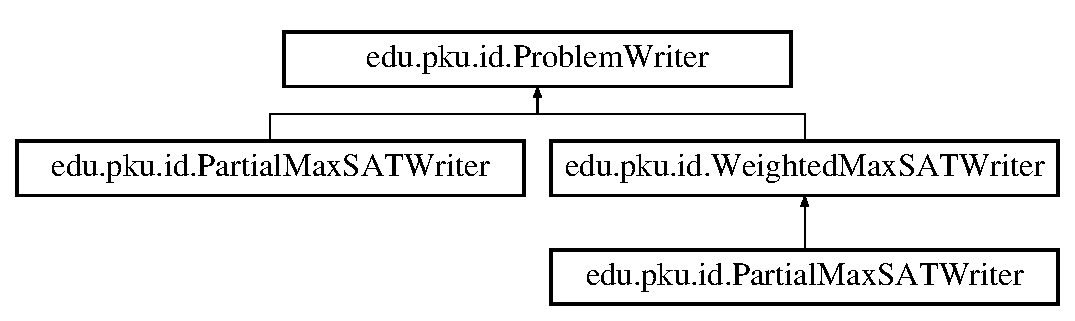
\includegraphics[height=3.000000cm]{interfaceedu_1_1pku_1_1id_1_1_problem_writer}
\end{center}
\end{figure}
\subsection*{Public Member Functions}
\begin{DoxyCompactItemize}
\item 
abstract void \hyperlink{interfaceedu_1_1pku_1_1id_1_1_problem_writer_aa2c5df4e6546cb6d7980d179cc8f91cd}{write} ()  throws IOException
\end{DoxyCompactItemize}


\subsection{Member Function Documentation}
\hypertarget{interfaceedu_1_1pku_1_1id_1_1_problem_writer_aa2c5df4e6546cb6d7980d179cc8f91cd}{
\index{edu::pku::id::ProblemWriter@{edu::pku::id::ProblemWriter}!write@{write}}
\index{write@{write}!edu::pku::id::ProblemWriter@{edu::pku::id::ProblemWriter}}
\subsubsection[{write}]{\setlength{\rightskip}{0pt plus 5cm}abstract void edu.pku.id.ProblemWriter.write (
\begin{DoxyParamCaption}
{}
\end{DoxyParamCaption}
)  throws IOException\hspace{0.3cm}{\ttfamily  \mbox{[}pure virtual\mbox{]}}}}
\label{interfaceedu_1_1pku_1_1id_1_1_problem_writer_aa2c5df4e6546cb6d7980d179cc8f91cd}


Implemented in \hyperlink{classedu_1_1pku_1_1id_1_1_weighted_max_s_a_t_writer_a9ca988f376b3618c2b6b4724feb6a9f5}{edu.pku.id.WeightedMaxSATWriter}.



The documentation for this interface was generated from the following file:\begin{DoxyCompactItemize}
\item 
src/edu/pku/id/\hyperlink{_problem_writer_8java}{ProblemWriter.java}\end{DoxyCompactItemize}

\hypertarget{classedu_1_1pku_1_1id_1_1_q_c_reasoner}{
\section{edu.pku.id.QCReasoner Class Reference}
\label{classedu_1_1pku_1_1id_1_1_q_c_reasoner}\index{edu::pku::id::QCReasoner@{edu::pku::id::QCReasoner}}
}
Inheritance diagram for edu.pku.id.QCReasoner:\begin{figure}[H]
\begin{center}
\leavevmode
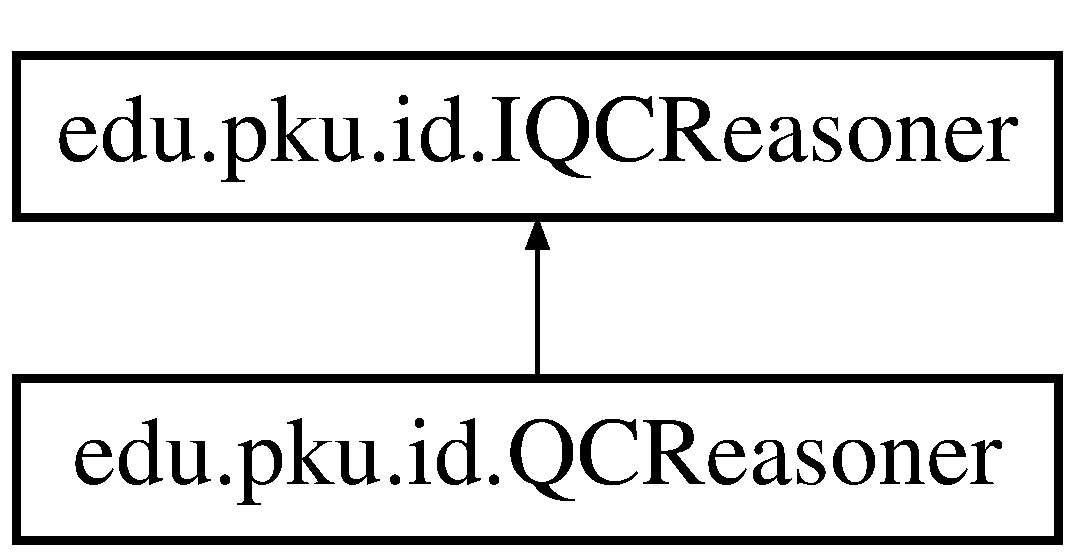
\includegraphics[height=2.000000cm]{classedu_1_1pku_1_1id_1_1_q_c_reasoner}
\end{center}
\end{figure}
\subsection*{Public Member Functions}
\begin{DoxyCompactItemize}
\item 
boolean \hyperlink{classedu_1_1pku_1_1id_1_1_q_c_reasoner_a0ce01daedfae2f88548978205d4848db}{qcEntails} (List$<$ IVecInt $>$ kb, IVecInt consequence)
\item 
boolean \hyperlink{classedu_1_1pku_1_1id_1_1_q_c_reasoner_a98bdf18d6a8222310060877e6cff6d80}{isQcModel} (List$<$ IVecInt $>$ kb, List$<$ \hyperlink{namespaceedu_1_1pku_1_1id_a01cdd35063021f272bd905de5f43f634}{TruthValue} $>$ model)
\item 
boolean \hyperlink{classedu_1_1pku_1_1id_1_1_q_c_reasoner_a63fc892ce36a74721446c691c60cdbd1}{isQcModel} (IVecInt clause, List$<$ \hyperlink{namespaceedu_1_1pku_1_1id_a01cdd35063021f272bd905de5f43f634}{TruthValue} $>$ interpretation)
\end{DoxyCompactItemize}
\subsection*{Private Member Functions}
\begin{DoxyCompactItemize}
\item 
List$<$ IVecInt $>$ \hyperlink{classedu_1_1pku_1_1id_1_1_q_c_reasoner_a11930b7f5e8427253338a98508fb1072}{strong} (List$<$ IVecInt $>$ clauses)
\item 
List$<$ IVecInt $>$ \hyperlink{classedu_1_1pku_1_1id_1_1_q_c_reasoner_ad841248cfd8f06335268248973876c17}{strong} (IVecInt clause)
\item 
List$<$ IVecInt $>$ \hyperlink{classedu_1_1pku_1_1id_1_1_q_c_reasoner_a52b070b2beb0989d50be56bb9d4864f0}{negWeak} (IVecInt clause)
\item 
int \hyperlink{classedu_1_1pku_1_1id_1_1_q_c_reasoner_a9dd63d2e49f6f5b53c4da1f74886708f}{literalPositiveTransform} (int literal)
\item 
int \hyperlink{classedu_1_1pku_1_1id_1_1_q_c_reasoner_aa2ab8c28775a0f950ea4932f056cc68e}{literalNegativeTransform} (int literal)
\item 
boolean \hyperlink{classedu_1_1pku_1_1id_1_1_q_c_reasoner_a96555b78c68cdc49f34d27ce44cdfdc1}{areClausesSatisfiable} (List$<$ IVecInt $>$ clauses)
\item 
List$<$ Boolean $>$ \hyperlink{classedu_1_1pku_1_1id_1_1_q_c_reasoner_aec484fe6e1aeaae5ba59f45da88a9f87}{asClassicModel} (List$<$ \hyperlink{namespaceedu_1_1pku_1_1id_a01cdd35063021f272bd905de5f43f634}{TruthValue} $>$ model)
\end{DoxyCompactItemize}
\subsection*{Static Private Attributes}
\begin{DoxyCompactItemize}
\item 
static final int \hyperlink{classedu_1_1pku_1_1id_1_1_q_c_reasoner_af0acf65658bdcdc6c8c4dc45652a85a9}{Z} = 3
\end{DoxyCompactItemize}


\subsection{Detailed Description}
Quasi Classical Logic Reasoner 准经典逻辑推理机 \par
 算法基于文献 Marquis, P., and Porquet, N. 2001. Computational aspects of quasi-\/classical entailment. {\itshape Journal of Applied Non-\/classical Logics\/} 11:295-\/312. \par
 同时使用了用引入新变量来避免变成CNF范式时的公式长度的指数膨胀的技巧 

\subsection{Member Function Documentation}
\hypertarget{classedu_1_1pku_1_1id_1_1_q_c_reasoner_a96555b78c68cdc49f34d27ce44cdfdc1}{
\index{edu::pku::id::QCReasoner@{edu::pku::id::QCReasoner}!areClausesSatisfiable@{areClausesSatisfiable}}
\index{areClausesSatisfiable@{areClausesSatisfiable}!edu::pku::id::QCReasoner@{edu::pku::id::QCReasoner}}
\subsubsection[{areClausesSatisfiable}]{\setlength{\rightskip}{0pt plus 5cm}boolean edu.pku.id.QCReasoner.areClausesSatisfiable (
\begin{DoxyParamCaption}
\item[{List$<$ IVecInt $>$}]{ clauses}
\end{DoxyParamCaption}
)\hspace{0.3cm}{\ttfamily  \mbox{[}private\mbox{]}}}}
\label{classedu_1_1pku_1_1id_1_1_q_c_reasoner_a96555b78c68cdc49f34d27ce44cdfdc1}
使用SAT4J推理机来检查子句集clauses的可满足性


\begin{DoxyParams}{Parameters}
{\em clauses} & \\
\hline
\end{DoxyParams}
\begin{DoxyReturn}{Returns}
子句集clauses的可满足性 
\end{DoxyReturn}
\hypertarget{classedu_1_1pku_1_1id_1_1_q_c_reasoner_aec484fe6e1aeaae5ba59f45da88a9f87}{
\index{edu::pku::id::QCReasoner@{edu::pku::id::QCReasoner}!asClassicModel@{asClassicModel}}
\index{asClassicModel@{asClassicModel}!edu::pku::id::QCReasoner@{edu::pku::id::QCReasoner}}
\subsubsection[{asClassicModel}]{\setlength{\rightskip}{0pt plus 5cm}List$<$Boolean$>$ edu.pku.id.QCReasoner.asClassicModel (
\begin{DoxyParamCaption}
\item[{List$<$ {\bf TruthValue} $>$}]{ model}
\end{DoxyParamCaption}
)\hspace{0.3cm}{\ttfamily  \mbox{[}private\mbox{]}}}}
\label{classedu_1_1pku_1_1id_1_1_q_c_reasoner_aec484fe6e1aeaae5ba59f45da88a9f87}

\begin{DoxyParams}{Parameters}
{\em model} & a QC interpretation \\
\hline
\end{DoxyParams}
\begin{DoxyReturn}{Returns}
a classical model 
\begin{DoxyItemize}
\item B -\/$>$ (t,t) 
\item t -\/$>$ (t,f) 
\item f -\/$>$ (f,t) 
\item N -\/$>$ (N,f) 
\end{DoxyItemize}
\end{DoxyReturn}
\hypertarget{classedu_1_1pku_1_1id_1_1_q_c_reasoner_a98bdf18d6a8222310060877e6cff6d80}{
\index{edu::pku::id::QCReasoner@{edu::pku::id::QCReasoner}!isQcModel@{isQcModel}}
\index{isQcModel@{isQcModel}!edu::pku::id::QCReasoner@{edu::pku::id::QCReasoner}}
\subsubsection[{isQcModel}]{\setlength{\rightskip}{0pt plus 5cm}boolean edu.pku.id.QCReasoner.isQcModel (
\begin{DoxyParamCaption}
\item[{List$<$ IVecInt $>$}]{ kb, }
\item[{List$<$ {\bf TruthValue} $>$}]{ model}
\end{DoxyParamCaption}
)\hspace{0.3cm}{\ttfamily  \mbox{[}virtual\mbox{]}}}}
\label{classedu_1_1pku_1_1id_1_1_q_c_reasoner_a98bdf18d6a8222310060877e6cff6d80}


Implements \hyperlink{interfaceedu_1_1pku_1_1id_1_1_i_q_c_reasoner_a4d1172287213bd0be63dbd75f047aa7c}{edu.pku.id.IQCReasoner}.

\hypertarget{classedu_1_1pku_1_1id_1_1_q_c_reasoner_a63fc892ce36a74721446c691c60cdbd1}{
\index{edu::pku::id::QCReasoner@{edu::pku::id::QCReasoner}!isQcModel@{isQcModel}}
\index{isQcModel@{isQcModel}!edu::pku::id::QCReasoner@{edu::pku::id::QCReasoner}}
\subsubsection[{isQcModel}]{\setlength{\rightskip}{0pt plus 5cm}boolean edu.pku.id.QCReasoner.isQcModel (
\begin{DoxyParamCaption}
\item[{IVecInt}]{ clause, }
\item[{List$<$ {\bf TruthValue} $>$}]{ interpretation}
\end{DoxyParamCaption}
)}}
\label{classedu_1_1pku_1_1id_1_1_q_c_reasoner_a63fc892ce36a74721446c691c60cdbd1}

\begin{DoxyParams}{Parameters}
{\em clause} & \\
\hline
{\em interpretation} & I $|$-\/Q l\_\-1   l\_\-n if I $|$-\/  (+l\_\-i   -\/l\_\-i)  ( +l\_\-i  -\/l\_\-i)\\
\hline
\end{DoxyParams}
\begin{DoxyReturn}{Returns}
whether {\ttfamily interpretation} is a QC model of {\ttfamily clause} 
\end{DoxyReturn}
\hypertarget{classedu_1_1pku_1_1id_1_1_q_c_reasoner_aa2ab8c28775a0f950ea4932f056cc68e}{
\index{edu::pku::id::QCReasoner@{edu::pku::id::QCReasoner}!literalNegativeTransform@{literalNegativeTransform}}
\index{literalNegativeTransform@{literalNegativeTransform}!edu::pku::id::QCReasoner@{edu::pku::id::QCReasoner}}
\subsubsection[{literalNegativeTransform}]{\setlength{\rightskip}{0pt plus 5cm}int edu.pku.id.QCReasoner.literalNegativeTransform (
\begin{DoxyParamCaption}
\item[{int}]{ literal}
\end{DoxyParamCaption}
)\hspace{0.3cm}{\ttfamily  \mbox{[}private\mbox{]}}}}
\label{classedu_1_1pku_1_1id_1_1_q_c_reasoner_aa2ab8c28775a0f950ea4932f056cc68e}
l -\/$>$ -\/l a -\/$>$ -\/a  a -\/$>$ +a \hypertarget{classedu_1_1pku_1_1id_1_1_q_c_reasoner_a9dd63d2e49f6f5b53c4da1f74886708f}{
\index{edu::pku::id::QCReasoner@{edu::pku::id::QCReasoner}!literalPositiveTransform@{literalPositiveTransform}}
\index{literalPositiveTransform@{literalPositiveTransform}!edu::pku::id::QCReasoner@{edu::pku::id::QCReasoner}}
\subsubsection[{literalPositiveTransform}]{\setlength{\rightskip}{0pt plus 5cm}int edu.pku.id.QCReasoner.literalPositiveTransform (
\begin{DoxyParamCaption}
\item[{int}]{ literal}
\end{DoxyParamCaption}
)\hspace{0.3cm}{\ttfamily  \mbox{[}private\mbox{]}}}}
\label{classedu_1_1pku_1_1id_1_1_q_c_reasoner_a9dd63d2e49f6f5b53c4da1f74886708f}
正原子a的编码如果是x +a的编码为4x -\/a的编码为4x+1

l -\/$>$ +l a -\/$>$ +a  a -\/$>$ -\/a \hypertarget{classedu_1_1pku_1_1id_1_1_q_c_reasoner_a52b070b2beb0989d50be56bb9d4864f0}{
\index{edu::pku::id::QCReasoner@{edu::pku::id::QCReasoner}!negWeak@{negWeak}}
\index{negWeak@{negWeak}!edu::pku::id::QCReasoner@{edu::pku::id::QCReasoner}}
\subsubsection[{negWeak}]{\setlength{\rightskip}{0pt plus 5cm}List$<$IVecInt$>$ edu.pku.id.QCReasoner.negWeak (
\begin{DoxyParamCaption}
\item[{IVecInt}]{ clause}
\end{DoxyParamCaption}
)\hspace{0.3cm}{\ttfamily  \mbox{[}private\mbox{]}}}}
\label{classedu_1_1pku_1_1id_1_1_q_c_reasoner_a52b070b2beb0989d50be56bb9d4864f0}
弱变换\par
 W(l\_\-1, , l\_\-n) = \{i=1\}$^\wedge$n +l\_\-i \par
 然后将其取反,由De Morgan律,变换为n个子句  +l\_\-i, i = 1, .. ,n


\begin{DoxyParams}{Parameters}
{\em clause} & \\
\hline
\end{DoxyParams}
\begin{DoxyReturn}{Returns}
弱变换的结果 
\end{DoxyReturn}
\hypertarget{classedu_1_1pku_1_1id_1_1_q_c_reasoner_a0ce01daedfae2f88548978205d4848db}{
\index{edu::pku::id::QCReasoner@{edu::pku::id::QCReasoner}!qcEntails@{qcEntails}}
\index{qcEntails@{qcEntails}!edu::pku::id::QCReasoner@{edu::pku::id::QCReasoner}}
\subsubsection[{qcEntails}]{\setlength{\rightskip}{0pt plus 5cm}boolean edu.pku.id.QCReasoner.qcEntails (
\begin{DoxyParamCaption}
\item[{List$<$ IVecInt $>$}]{ kb, }
\item[{IVecInt}]{ consequence}
\end{DoxyParamCaption}
)\hspace{0.3cm}{\ttfamily  \mbox{[}virtual\mbox{]}}}}
\label{classedu_1_1pku_1_1id_1_1_q_c_reasoner_a0ce01daedfae2f88548978205d4848db}
检测kb是否能够QC蕴含gamma


\begin{DoxyParams}{Parameters}
{\em kb} & 前提知识库,表示为子句的集合 \\
\hline
{\em consequence} & 结论,表示为子句 \\
\hline
\end{DoxyParams}
\begin{DoxyReturn}{Returns}
是否能够QC蕴含 
\end{DoxyReturn}


Implements \hyperlink{interfaceedu_1_1pku_1_1id_1_1_i_q_c_reasoner_a2cf3cc08877e6d06485e758bdbf5bf94}{edu.pku.id.IQCReasoner}.

\hypertarget{classedu_1_1pku_1_1id_1_1_q_c_reasoner_ad841248cfd8f06335268248973876c17}{
\index{edu::pku::id::QCReasoner@{edu::pku::id::QCReasoner}!strong@{strong}}
\index{strong@{strong}!edu::pku::id::QCReasoner@{edu::pku::id::QCReasoner}}
\subsubsection[{strong}]{\setlength{\rightskip}{0pt plus 5cm}List$<$IVecInt$>$ edu.pku.id.QCReasoner.strong (
\begin{DoxyParamCaption}
\item[{IVecInt}]{ clause}
\end{DoxyParamCaption}
)\hspace{0.3cm}{\ttfamily  \mbox{[}private\mbox{]}}}}
\label{classedu_1_1pku_1_1id_1_1_q_c_reasoner_ad841248cfd8f06335268248973876c17}
将一个子句进行强变换\par
 算法如下:\par
 S(l\_\-1   l\_\-n) = \{i=1\}$^\wedge$n(+l\_\-i  -\/ l\_\-i)  \{i=1\}$^\wedge$n(+l\_\-i -\/l\_\-i)\par
 引入新变量,来避免变换后的长度发生指数爆炸\par
 y\_\-i $<$-\/ +l\_\-i  -\/ l\_\-i, i = 1, , n\par
 z $<$-\/ \{i=1\}$^\wedge$n(+l\_\-i -\/l\_\-i)\par
 这样在保持可满足性下,可以变换为\par
 (\{i=1\}$^\wedge$n y\_\-i  z)  \{i=1\}$^\wedge$n( y\_\-i  +l\_\-i)  \{i=1\}$^\wedge$n( y\_\-i   -\/l\_\-i) \{i=1\}$^\wedge$n( z  +l\_\-i)  \{i=1\}$^\wedge$n( z  -\/ l\_\-i)

保证可满足性的变换中引入的 y\_\-i = +l\_\-i   -\/ l\_\-i的编码为4x+2 引入的z = \{i=1\}$^\wedge$n (+l\_\-i  -\/l\_\-i) 的编码为3


\begin{DoxyParams}{Parameters}
{\em clause} & 要变换的子句 \\
\hline
\end{DoxyParams}
\begin{DoxyReturn}{Returns}
强变换的结果 
\end{DoxyReturn}
\hypertarget{classedu_1_1pku_1_1id_1_1_q_c_reasoner_a11930b7f5e8427253338a98508fb1072}{
\index{edu::pku::id::QCReasoner@{edu::pku::id::QCReasoner}!strong@{strong}}
\index{strong@{strong}!edu::pku::id::QCReasoner@{edu::pku::id::QCReasoner}}
\subsubsection[{strong}]{\setlength{\rightskip}{0pt plus 5cm}List$<$IVecInt$>$ edu.pku.id.QCReasoner.strong (
\begin{DoxyParamCaption}
\item[{List$<$ IVecInt $>$}]{ clauses}
\end{DoxyParamCaption}
)\hspace{0.3cm}{\ttfamily  \mbox{[}private\mbox{]}}}}
\label{classedu_1_1pku_1_1id_1_1_q_c_reasoner_a11930b7f5e8427253338a98508fb1072}
将一个子句集进行强变换 S() = \{clause  in \} S()


\begin{DoxyParams}{Parameters}
{\em clauses} & 子句集 \\
\hline
\end{DoxyParams}
\begin{DoxyReturn}{Returns}
强变换的结果 
\end{DoxyReturn}


\subsection{Member Data Documentation}
\hypertarget{classedu_1_1pku_1_1id_1_1_q_c_reasoner_af0acf65658bdcdc6c8c4dc45652a85a9}{
\index{edu::pku::id::QCReasoner@{edu::pku::id::QCReasoner}!Z@{Z}}
\index{Z@{Z}!edu::pku::id::QCReasoner@{edu::pku::id::QCReasoner}}
\subsubsection[{Z}]{\setlength{\rightskip}{0pt plus 5cm}final int {\bf edu.pku.id.QCReasoner.Z} = 3\hspace{0.3cm}{\ttfamily  \mbox{[}static, private\mbox{]}}}}
\label{classedu_1_1pku_1_1id_1_1_q_c_reasoner_af0acf65658bdcdc6c8c4dc45652a85a9}


The documentation for this class was generated from the following file:\begin{DoxyCompactItemize}
\item 
src/edu/pku/id/\hyperlink{_q_c_reasoner_8java}{QCReasoner.java}\end{DoxyCompactItemize}

\hypertarget{classedu_1_1pku_1_1id_1_1_q_c_reasoner_v2}{
\section{edu.pku.id.QCReasonerV2 Class Reference}
\label{classedu_1_1pku_1_1id_1_1_q_c_reasoner_v2}\index{edu::pku::id::QCReasonerV2@{edu::pku::id::QCReasonerV2}}
}
Inheritance diagram for edu.pku.id.QCReasonerV2:\begin{figure}[H]
\begin{center}
\leavevmode
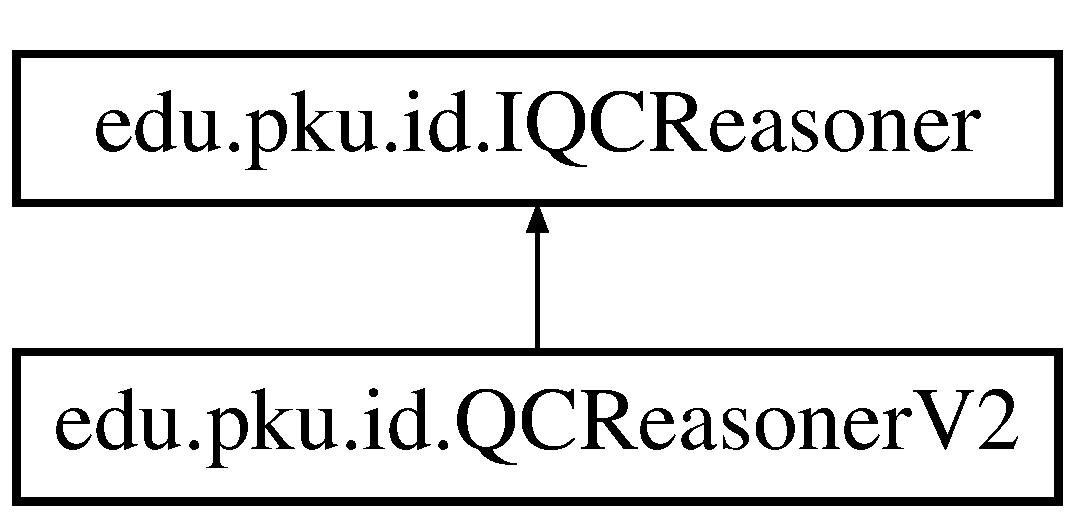
\includegraphics[height=2.000000cm]{classedu_1_1pku_1_1id_1_1_q_c_reasoner_v2}
\end{center}
\end{figure}
\subsection*{Public Member Functions}
\begin{DoxyCompactItemize}
\item 
boolean \hyperlink{classedu_1_1pku_1_1id_1_1_q_c_reasoner_v2_a04f22e9cef82ae44d46179d252ad46ef}{qcEntails} (List$<$ IVecInt $>$ kb, IVecInt consequence)
\end{DoxyCompactItemize}
\subsection*{Static Public Member Functions}
\begin{DoxyCompactItemize}
\item 
static void \hyperlink{classedu_1_1pku_1_1id_1_1_q_c_reasoner_v2_aa807c5199d238766a245fdc389369808}{main} (String\mbox{[}$\,$\mbox{]} args)
\end{DoxyCompactItemize}
\subsection*{Private Member Functions}
\begin{DoxyCompactItemize}
\item 
List$<$ IVecInt $>$ \hyperlink{classedu_1_1pku_1_1id_1_1_q_c_reasoner_v2_a2287ecfa0c316caad00288a00d99a53d}{strong} (List$<$ IVecInt $>$ clauses)
\item 
List$<$ IVecInt $>$ \hyperlink{classedu_1_1pku_1_1id_1_1_q_c_reasoner_v2_a58d1acccb28e5b185e6af32958deff3b}{strong} (IVecInt clause)
\item 
List$<$ IVecInt $>$ \hyperlink{classedu_1_1pku_1_1id_1_1_q_c_reasoner_v2_a9fcf948861f95fc5bf1451c22737fb46}{negWeak} (IVecInt clause)
\item 
int \hyperlink{classedu_1_1pku_1_1id_1_1_q_c_reasoner_v2_a1523c6684bc8b1cf7267a5f86413d481}{literalPositiveTransform} (int literal)
\item 
int \hyperlink{classedu_1_1pku_1_1id_1_1_q_c_reasoner_v2_a965973948f1b741cca0a01010b8210d0}{literalNegativeTransform} (int literal)
\item 
boolean \hyperlink{classedu_1_1pku_1_1id_1_1_q_c_reasoner_v2_abe75137424ee56f6c3ffe02c6d3ef137}{areClausesSatisfiable} (List$<$ IVecInt $>$ clauses)
\end{DoxyCompactItemize}
\subsection*{Static Private Attributes}
\begin{DoxyCompactItemize}
\item 
static final int \hyperlink{classedu_1_1pku_1_1id_1_1_q_c_reasoner_v2_af2c8bff8769fa861fbb3d224d8fdf7c3}{Z} = 3
\end{DoxyCompactItemize}


\subsection{Detailed Description}
Quasi Classical Logic Reasoner 准经典逻辑推理机 \par
 算法基于文献 Marquis, P., and Porquet, N. 2001. Computational aspects of quasi-\/classical entailment. {\itshape Journal of Applied Non-\/classical Logics\/} 11:295-\/312. \par
 

\subsection{Member Function Documentation}
\hypertarget{classedu_1_1pku_1_1id_1_1_q_c_reasoner_v2_abe75137424ee56f6c3ffe02c6d3ef137}{
\index{edu::pku::id::QCReasonerV2@{edu::pku::id::QCReasonerV2}!areClausesSatisfiable@{areClausesSatisfiable}}
\index{areClausesSatisfiable@{areClausesSatisfiable}!edu::pku::id::QCReasonerV2@{edu::pku::id::QCReasonerV2}}
\subsubsection[{areClausesSatisfiable}]{\setlength{\rightskip}{0pt plus 5cm}boolean edu.pku.id.QCReasonerV2.areClausesSatisfiable (
\begin{DoxyParamCaption}
\item[{List$<$ IVecInt $>$}]{ clauses}
\end{DoxyParamCaption}
)\hspace{0.3cm}{\ttfamily  \mbox{[}private\mbox{]}}}}
\label{classedu_1_1pku_1_1id_1_1_q_c_reasoner_v2_abe75137424ee56f6c3ffe02c6d3ef137}
使用SAT4J推理机来检查子句集clauses的可满足性 
\begin{DoxyParams}{Parameters}
{\em clauses} & \\
\hline
\end{DoxyParams}
\begin{DoxyReturn}{Returns}
子句集clauses的可满足性 
\end{DoxyReturn}
\hypertarget{classedu_1_1pku_1_1id_1_1_q_c_reasoner_v2_a965973948f1b741cca0a01010b8210d0}{
\index{edu::pku::id::QCReasonerV2@{edu::pku::id::QCReasonerV2}!literalNegativeTransform@{literalNegativeTransform}}
\index{literalNegativeTransform@{literalNegativeTransform}!edu::pku::id::QCReasonerV2@{edu::pku::id::QCReasonerV2}}
\subsubsection[{literalNegativeTransform}]{\setlength{\rightskip}{0pt plus 5cm}int edu.pku.id.QCReasonerV2.literalNegativeTransform (
\begin{DoxyParamCaption}
\item[{int}]{ literal}
\end{DoxyParamCaption}
)\hspace{0.3cm}{\ttfamily  \mbox{[}private\mbox{]}}}}
\label{classedu_1_1pku_1_1id_1_1_q_c_reasoner_v2_a965973948f1b741cca0a01010b8210d0}
l -\/$>$ -\/l a -\/$>$ -\/a  a -\/$>$ +a \hypertarget{classedu_1_1pku_1_1id_1_1_q_c_reasoner_v2_a1523c6684bc8b1cf7267a5f86413d481}{
\index{edu::pku::id::QCReasonerV2@{edu::pku::id::QCReasonerV2}!literalPositiveTransform@{literalPositiveTransform}}
\index{literalPositiveTransform@{literalPositiveTransform}!edu::pku::id::QCReasonerV2@{edu::pku::id::QCReasonerV2}}
\subsubsection[{literalPositiveTransform}]{\setlength{\rightskip}{0pt plus 5cm}int edu.pku.id.QCReasonerV2.literalPositiveTransform (
\begin{DoxyParamCaption}
\item[{int}]{ literal}
\end{DoxyParamCaption}
)\hspace{0.3cm}{\ttfamily  \mbox{[}private\mbox{]}}}}
\label{classedu_1_1pku_1_1id_1_1_q_c_reasoner_v2_a1523c6684bc8b1cf7267a5f86413d481}
正原子a的编码如果是x +a的编码为4x -\/a的编码为4x+1

l -\/$>$ +l a -\/$>$ +a  a -\/$>$ -\/a \hypertarget{classedu_1_1pku_1_1id_1_1_q_c_reasoner_v2_aa807c5199d238766a245fdc389369808}{
\index{edu::pku::id::QCReasonerV2@{edu::pku::id::QCReasonerV2}!main@{main}}
\index{main@{main}!edu::pku::id::QCReasonerV2@{edu::pku::id::QCReasonerV2}}
\subsubsection[{main}]{\setlength{\rightskip}{0pt plus 5cm}static void edu.pku.id.QCReasonerV2.main (
\begin{DoxyParamCaption}
\item[{String\mbox{[}$\,$\mbox{]}}]{ args}
\end{DoxyParamCaption}
)\hspace{0.3cm}{\ttfamily  \mbox{[}static\mbox{]}}}}
\label{classedu_1_1pku_1_1id_1_1_q_c_reasoner_v2_aa807c5199d238766a245fdc389369808}
\hypertarget{classedu_1_1pku_1_1id_1_1_q_c_reasoner_v2_a9fcf948861f95fc5bf1451c22737fb46}{
\index{edu::pku::id::QCReasonerV2@{edu::pku::id::QCReasonerV2}!negWeak@{negWeak}}
\index{negWeak@{negWeak}!edu::pku::id::QCReasonerV2@{edu::pku::id::QCReasonerV2}}
\subsubsection[{negWeak}]{\setlength{\rightskip}{0pt plus 5cm}List$<$IVecInt$>$ edu.pku.id.QCReasonerV2.negWeak (
\begin{DoxyParamCaption}
\item[{IVecInt}]{ clause}
\end{DoxyParamCaption}
)\hspace{0.3cm}{\ttfamily  \mbox{[}private\mbox{]}}}}
\label{classedu_1_1pku_1_1id_1_1_q_c_reasoner_v2_a9fcf948861f95fc5bf1451c22737fb46}
弱变换\par
 W(l\_\-1, , l\_\-n) = \{i=1\}$^\wedge$n +l\_\-i \par
 然后将其取反,由De Morgan律,变换为n个子句  +l\_\-i, i = 1, .. ,n 
\begin{DoxyParams}{Parameters}
{\em clause} & \\
\hline
\end{DoxyParams}
\begin{DoxyReturn}{Returns}
弱变换的结果 
\end{DoxyReturn}
\hypertarget{classedu_1_1pku_1_1id_1_1_q_c_reasoner_v2_a04f22e9cef82ae44d46179d252ad46ef}{
\index{edu::pku::id::QCReasonerV2@{edu::pku::id::QCReasonerV2}!qcEntails@{qcEntails}}
\index{qcEntails@{qcEntails}!edu::pku::id::QCReasonerV2@{edu::pku::id::QCReasonerV2}}
\subsubsection[{qcEntails}]{\setlength{\rightskip}{0pt plus 5cm}boolean edu.pku.id.QCReasonerV2.qcEntails (
\begin{DoxyParamCaption}
\item[{List$<$ IVecInt $>$}]{ kb, }
\item[{IVecInt}]{ consequence}
\end{DoxyParamCaption}
)\hspace{0.3cm}{\ttfamily  \mbox{[}virtual\mbox{]}}}}
\label{classedu_1_1pku_1_1id_1_1_q_c_reasoner_v2_a04f22e9cef82ae44d46179d252ad46ef}
检测kb是否能够QC蕴含gamma


\begin{DoxyParams}{Parameters}
{\em kb} & 前提知识库,表示为子句的集合 \\
\hline
{\em consequence} & 结论,表示为子句 \\
\hline
\end{DoxyParams}
\begin{DoxyReturn}{Returns}
是否能够QC蕴含 
\end{DoxyReturn}


Implements \hyperlink{interfaceedu_1_1pku_1_1id_1_1_i_q_c_reasoner_a2cf3cc08877e6d06485e758bdbf5bf94}{edu.pku.id.IQCReasoner}.

\hypertarget{classedu_1_1pku_1_1id_1_1_q_c_reasoner_v2_a2287ecfa0c316caad00288a00d99a53d}{
\index{edu::pku::id::QCReasonerV2@{edu::pku::id::QCReasonerV2}!strong@{strong}}
\index{strong@{strong}!edu::pku::id::QCReasonerV2@{edu::pku::id::QCReasonerV2}}
\subsubsection[{strong}]{\setlength{\rightskip}{0pt plus 5cm}List$<$IVecInt$>$ edu.pku.id.QCReasonerV2.strong (
\begin{DoxyParamCaption}
\item[{List$<$ IVecInt $>$}]{ clauses}
\end{DoxyParamCaption}
)\hspace{0.3cm}{\ttfamily  \mbox{[}private\mbox{]}}}}
\label{classedu_1_1pku_1_1id_1_1_q_c_reasoner_v2_a2287ecfa0c316caad00288a00d99a53d}
将一个子句集进行强变换 S() = \{clause  in \} S() 
\begin{DoxyParams}{Parameters}
{\em clauses} & 子句集 \\
\hline
\end{DoxyParams}
\begin{DoxyReturn}{Returns}
强变换的结果 
\end{DoxyReturn}
\hypertarget{classedu_1_1pku_1_1id_1_1_q_c_reasoner_v2_a58d1acccb28e5b185e6af32958deff3b}{
\index{edu::pku::id::QCReasonerV2@{edu::pku::id::QCReasonerV2}!strong@{strong}}
\index{strong@{strong}!edu::pku::id::QCReasonerV2@{edu::pku::id::QCReasonerV2}}
\subsubsection[{strong}]{\setlength{\rightskip}{0pt plus 5cm}List$<$IVecInt$>$ edu.pku.id.QCReasonerV2.strong (
\begin{DoxyParamCaption}
\item[{IVecInt}]{ clause}
\end{DoxyParamCaption}
)\hspace{0.3cm}{\ttfamily  \mbox{[}private\mbox{]}}}}
\label{classedu_1_1pku_1_1id_1_1_q_c_reasoner_v2_a58d1acccb28e5b185e6af32958deff3b}
将一个子句进行强变换\par
 算法如下:\par
 S(l\_\-1,,l\_\-n) = (+l\_\-1  +l\_\-2   +l\_\-n)  ( -\/l\_\-1  +l\_\-2   +l\_\-n)  (   -\/l\_\-2   +l\_\-n)    (  +l\_\-2    -\/l\_\-n) 
\begin{DoxyParams}{Parameters}
{\em clause} & 要变换的子句 \\
\hline
\end{DoxyParams}
\begin{DoxyReturn}{Returns}
强变换的结果 
\end{DoxyReturn}


\subsection{Member Data Documentation}
\hypertarget{classedu_1_1pku_1_1id_1_1_q_c_reasoner_v2_af2c8bff8769fa861fbb3d224d8fdf7c3}{
\index{edu::pku::id::QCReasonerV2@{edu::pku::id::QCReasonerV2}!Z@{Z}}
\index{Z@{Z}!edu::pku::id::QCReasonerV2@{edu::pku::id::QCReasonerV2}}
\subsubsection[{Z}]{\setlength{\rightskip}{0pt plus 5cm}final int {\bf edu.pku.id.QCReasonerV2.Z} = 3\hspace{0.3cm}{\ttfamily  \mbox{[}static, private\mbox{]}}}}
\label{classedu_1_1pku_1_1id_1_1_q_c_reasoner_v2_af2c8bff8769fa861fbb3d224d8fdf7c3}


The documentation for this class was generated from the following file:\begin{DoxyCompactItemize}
\item 
src/edu/pku/id/\hyperlink{_q_c_reasoner_v2_8java}{QCReasonerV2.java}\end{DoxyCompactItemize}

\hypertarget{classedu_1_1pku_1_1id_1_1_q_c_translater}{
\section{edu.pku.id.QCTranslater Class Reference}
\label{classedu_1_1pku_1_1id_1_1_q_c_translater}\index{edu::pku::id::QCTranslater@{edu::pku::id::QCTranslater}}
}
Inheritance diagram for edu.pku.id.QCTranslater:\begin{figure}[H]
\begin{center}
\leavevmode
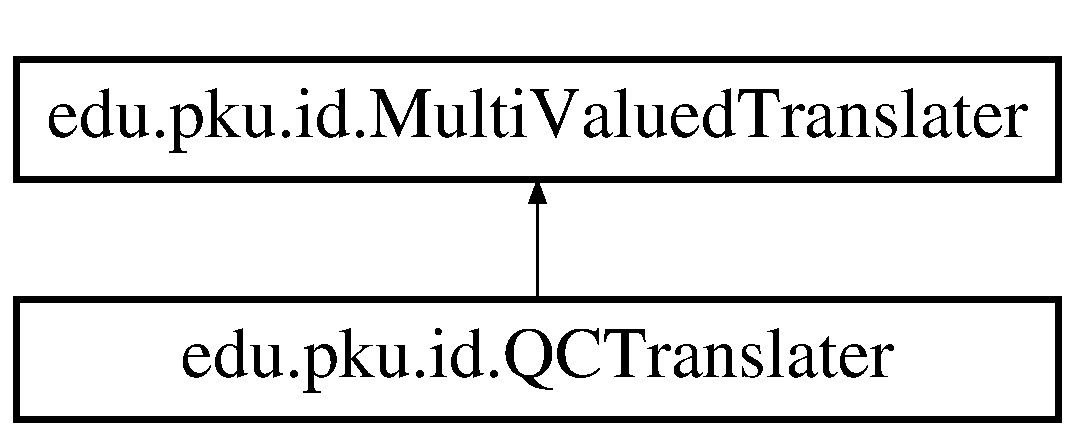
\includegraphics[height=2.000000cm]{classedu_1_1pku_1_1id_1_1_q_c_translater}
\end{center}
\end{figure}
\subsection*{Package Functions}
\begin{DoxyCompactItemize}
\item 
int \hyperlink{classedu_1_1pku_1_1id_1_1_q_c_translater_aa8bd352645be8437d8feda2f04aff560}{literalPositiveTransform} (int literal)
\item 
int \hyperlink{classedu_1_1pku_1_1id_1_1_q_c_translater_a9439713e9f21664274a144214507c17b}{literalNegativeTransform} (int literal)
\item 
void \hyperlink{classedu_1_1pku_1_1id_1_1_q_c_translater_a2b3b851d0bcb6cbfc07badd6e6434096}{translate} ()
\end{DoxyCompactItemize}
\subsection*{Package Attributes}
\begin{DoxyCompactItemize}
\item 
int \hyperlink{classedu_1_1pku_1_1id_1_1_q_c_translater_ab609761f32dc4ff41071cd17a5152798}{clauseIndex} = 0
\end{DoxyCompactItemize}
\subsection*{Private Member Functions}
\begin{DoxyCompactItemize}
\item 
List$<$ IVecInt $>$ \hyperlink{classedu_1_1pku_1_1id_1_1_q_c_translater_ab5f9bf3cb3a91a4b74ca8a8580468305}{translateClause} (IVecInt clause)
\item 
int \hyperlink{classedu_1_1pku_1_1id_1_1_q_c_translater_a09e237ebaa40f125c9eefbab1a6a567e}{z} (int index)
\item 
int \hyperlink{classedu_1_1pku_1_1id_1_1_q_c_translater_a608a6c46bf90a6a1edb5fd832e4e0806}{y} (int literal)
\end{DoxyCompactItemize}


\subsection{Member Function Documentation}
\hypertarget{classedu_1_1pku_1_1id_1_1_q_c_translater_a9439713e9f21664274a144214507c17b}{
\index{edu::pku::id::QCTranslater@{edu::pku::id::QCTranslater}!literalNegativeTransform@{literalNegativeTransform}}
\index{literalNegativeTransform@{literalNegativeTransform}!edu::pku::id::QCTranslater@{edu::pku::id::QCTranslater}}
\subsubsection[{literalNegativeTransform}]{\setlength{\rightskip}{0pt plus 5cm}int edu.pku.id.QCTranslater.literalNegativeTransform (
\begin{DoxyParamCaption}
\item[{int}]{ literal}
\end{DoxyParamCaption}
)\hspace{0.3cm}{\ttfamily  \mbox{[}package\mbox{]}}}}
\label{classedu_1_1pku_1_1id_1_1_q_c_translater_a9439713e9f21664274a144214507c17b}
l -\/$>$ -\/l a -\/$>$ -\/a  a -\/$>$ +a \hypertarget{classedu_1_1pku_1_1id_1_1_q_c_translater_aa8bd352645be8437d8feda2f04aff560}{
\index{edu::pku::id::QCTranslater@{edu::pku::id::QCTranslater}!literalPositiveTransform@{literalPositiveTransform}}
\index{literalPositiveTransform@{literalPositiveTransform}!edu::pku::id::QCTranslater@{edu::pku::id::QCTranslater}}
\subsubsection[{literalPositiveTransform}]{\setlength{\rightskip}{0pt plus 5cm}int edu.pku.id.QCTranslater.literalPositiveTransform (
\begin{DoxyParamCaption}
\item[{int}]{ literal}
\end{DoxyParamCaption}
)\hspace{0.3cm}{\ttfamily  \mbox{[}package\mbox{]}}}}
\label{classedu_1_1pku_1_1id_1_1_q_c_translater_aa8bd352645be8437d8feda2f04aff560}
姝e師瀛恆鐨勭紪鐮佸鏋滄槸x\par
 +a鐨勭紪鐮佷负4x\par
 -\/a鐨勭紪鐮佷负4x+1\par


l -\/$>$ +l\par
 a -\/$>$ +a\par
  a -\/$>$ -\/a\par
 \hypertarget{classedu_1_1pku_1_1id_1_1_q_c_translater_a2b3b851d0bcb6cbfc07badd6e6434096}{
\index{edu::pku::id::QCTranslater@{edu::pku::id::QCTranslater}!translate@{translate}}
\index{translate@{translate}!edu::pku::id::QCTranslater@{edu::pku::id::QCTranslater}}
\subsubsection[{translate}]{\setlength{\rightskip}{0pt plus 5cm}void edu.pku.id.QCTranslater.translate (
\begin{DoxyParamCaption}
{}
\end{DoxyParamCaption}
)\hspace{0.3cm}{\ttfamily  \mbox{[}package, virtual\mbox{]}}}}
\label{classedu_1_1pku_1_1id_1_1_q_c_translater_a2b3b851d0bcb6cbfc07badd6e6434096}


Implements \hyperlink{classedu_1_1pku_1_1id_1_1_multi_valued_translater_a57e687a8b1c011fb7c0ccbd72272e328}{edu.pku.id.MultiValuedTranslater}.

\hypertarget{classedu_1_1pku_1_1id_1_1_q_c_translater_ab5f9bf3cb3a91a4b74ca8a8580468305}{
\index{edu::pku::id::QCTranslater@{edu::pku::id::QCTranslater}!translateClause@{translateClause}}
\index{translateClause@{translateClause}!edu::pku::id::QCTranslater@{edu::pku::id::QCTranslater}}
\subsubsection[{translateClause}]{\setlength{\rightskip}{0pt plus 5cm}List$<$IVecInt$>$ edu.pku.id.QCTranslater.translateClause (
\begin{DoxyParamCaption}
\item[{IVecInt}]{ clause}
\end{DoxyParamCaption}
)\hspace{0.3cm}{\ttfamily  \mbox{[}private\mbox{]}}}}
\label{classedu_1_1pku_1_1id_1_1_q_c_translater_ab5f9bf3cb3a91a4b74ca8a8580468305}
灏嗕竴涓瓙鍙ヨ繘琛屽己鍙樻崲\par
 绠楁硶濡備笅:\par
 S(l\_\-1   l\_\-n) = \{i=1\}$^\wedge$n(+l\_\-i  -\/ l\_\-i)  \{i=1\}$^\wedge$n(+l\_\-i -\/l\_\-i)\par
 寮曞叆鏂板彉閲�鏉ラ伩鍏嶅彉鎹㈠悗鐨勯暱搴﹀彂鐢熸寚鏁扮垎鐐�br/$>$ y\_\-i $<$-\/ +l\_\-i  -\/ l\_\-i, i = 1, , n\par
 z $<$-\/ \{i=1\}$^\wedge$n(+l\_\-i -\/l\_\-i)\par
 杩欐牱鍦ㄤ繚鎸佸彲婊¤冻鎬т笅,鍙互鍙樻崲涓�br/$>$ (\{i=1\}$^\wedge$n y\_\-i  z)  \{i=1\}$^\wedge$n( y\_\-i  +l\_\-i)  \{i=1\}$^\wedge$n( y\_\-i   -\/l\_\-i) \{i=1\}$^\wedge$n( z  +l\_\-i)  \{i=1\}$^\wedge$n( z  -\/ l\_\-i)

淇濊瘉鍙弧瓒虫�鐨勫彉鎹腑寮曞叆鐨�y\_\-i = +l\_\-i   -\/ l\_\-i鐨勭紪鐮佷负4x+2 寮曞叆鐨剒 = \{i=1\}$^\wedge$n (+l\_\-i  -\/l\_\-i) 鐨勭紪鐮佷负3


\begin{DoxyParams}{Parameters}
{\em clause} & 瑕佸彉鎹㈢殑瀛愬彞 \\
\hline
\end{DoxyParams}
\begin{DoxyReturn}{Returns}
寮哄彉鎹㈢殑缁撴灉 
\end{DoxyReturn}
\hypertarget{classedu_1_1pku_1_1id_1_1_q_c_translater_a608a6c46bf90a6a1edb5fd832e4e0806}{
\index{edu::pku::id::QCTranslater@{edu::pku::id::QCTranslater}!y@{y}}
\index{y@{y}!edu::pku::id::QCTranslater@{edu::pku::id::QCTranslater}}
\subsubsection[{y}]{\setlength{\rightskip}{0pt plus 5cm}int edu.pku.id.QCTranslater.y (
\begin{DoxyParamCaption}
\item[{int}]{ literal}
\end{DoxyParamCaption}
)\hspace{0.3cm}{\ttfamily  \mbox{[}private\mbox{]}}}}
\label{classedu_1_1pku_1_1id_1_1_q_c_translater_a608a6c46bf90a6a1edb5fd832e4e0806}
\hypertarget{classedu_1_1pku_1_1id_1_1_q_c_translater_a09e237ebaa40f125c9eefbab1a6a567e}{
\index{edu::pku::id::QCTranslater@{edu::pku::id::QCTranslater}!z@{z}}
\index{z@{z}!edu::pku::id::QCTranslater@{edu::pku::id::QCTranslater}}
\subsubsection[{z}]{\setlength{\rightskip}{0pt plus 5cm}int edu.pku.id.QCTranslater.z (
\begin{DoxyParamCaption}
\item[{int}]{ index}
\end{DoxyParamCaption}
)\hspace{0.3cm}{\ttfamily  \mbox{[}private\mbox{]}}}}
\label{classedu_1_1pku_1_1id_1_1_q_c_translater_a09e237ebaa40f125c9eefbab1a6a567e}


\subsection{Member Data Documentation}
\hypertarget{classedu_1_1pku_1_1id_1_1_q_c_translater_ab609761f32dc4ff41071cd17a5152798}{
\index{edu::pku::id::QCTranslater@{edu::pku::id::QCTranslater}!clauseIndex@{clauseIndex}}
\index{clauseIndex@{clauseIndex}!edu::pku::id::QCTranslater@{edu::pku::id::QCTranslater}}
\subsubsection[{clauseIndex}]{\setlength{\rightskip}{0pt plus 5cm}int {\bf edu.pku.id.QCTranslater.clauseIndex} = 0\hspace{0.3cm}{\ttfamily  \mbox{[}package\mbox{]}}}}
\label{classedu_1_1pku_1_1id_1_1_q_c_translater_ab609761f32dc4ff41071cd17a5152798}


The documentation for this class was generated from the following file:\begin{DoxyCompactItemize}
\item 
src/edu/pku/id/\hyperlink{_q_c_translater_8java}{QCTranslater.java}\end{DoxyCompactItemize}

\hypertarget{classedu_1_1pku_1_1id_1_1cli_1_1_result_model_reader}{
\section{edu.pku.id.cli.ResultModelReader Class Reference}
\label{classedu_1_1pku_1_1id_1_1cli_1_1_result_model_reader}\index{edu::pku::id::cli::ResultModelReader@{edu::pku::id::cli::ResultModelReader}}
}
\subsection*{Public Member Functions}
\begin{DoxyCompactItemize}
\item 
\hyperlink{classedu_1_1pku_1_1id_1_1cli_1_1_result_model_reader_ab8e7736607cf9b562ff875ddb8d74c2c}{ResultModelReader} (String fileName)  throws FileNotFoundException 
\item 
double \hyperlink{classedu_1_1pku_1_1id_1_1cli_1_1_result_model_reader_a02a2080025d02a493b189390a4621921}{getIncDegree} ()  throws IOException, ParseFormatException 
\end{DoxyCompactItemize}
\subsection*{Static Public Member Functions}
\begin{DoxyCompactItemize}
\item 
static void \hyperlink{classedu_1_1pku_1_1id_1_1cli_1_1_result_model_reader_af394e32ff1c7eb3f05cecbf3283ae5bc}{main} (String args\mbox{[}$\,$\mbox{]})  throws IOException, ParseFormatException 
\end{DoxyCompactItemize}
\subsection*{Package Functions}
\begin{DoxyCompactItemize}
\item 
List$<$ Integer $>$ \hyperlink{classedu_1_1pku_1_1id_1_1cli_1_1_result_model_reader_a22451691cab76d90ca75d31fb6963e26}{getModel} ()  throws IOException 
\end{DoxyCompactItemize}
\subsection*{Package Attributes}
\begin{DoxyCompactItemize}
\item 
\hyperlink{classedu_1_1pku_1_1id_1_1_cnf_file_reader}{CnfFileReader} \hyperlink{classedu_1_1pku_1_1id_1_1cli_1_1_result_model_reader_a187962842c15d8aa1f28cc70cfd2bc6a}{cnfFileReader}
\end{DoxyCompactItemize}
\subsection*{Static Package Attributes}
\begin{DoxyCompactItemize}
\item 
static final Logger \hyperlink{classedu_1_1pku_1_1id_1_1cli_1_1_result_model_reader_a500bdcf07a976b25e65bc5c7ddf3db55}{logger} = LoggerFactory.getLogger(ResultModelReader.class)
\end{DoxyCompactItemize}
\subsection*{Private Member Functions}
\begin{DoxyCompactItemize}
\item 
int \hyperlink{classedu_1_1pku_1_1id_1_1cli_1_1_result_model_reader_aa031598959036fdd115e827dd4c8c756}{getVarsCount} ()  throws IOException, ParseFormatException 
\end{DoxyCompactItemize}
\subsection*{Private Attributes}
\begin{DoxyCompactItemize}
\item 
BufferedReader \hyperlink{classedu_1_1pku_1_1id_1_1cli_1_1_result_model_reader_ae26076ae9ffd55117eb4c135e68bbbd0}{modelReader}
\end{DoxyCompactItemize}


\subsection{Constructor \& Destructor Documentation}
\hypertarget{classedu_1_1pku_1_1id_1_1cli_1_1_result_model_reader_ab8e7736607cf9b562ff875ddb8d74c2c}{
\index{edu::pku::id::cli::ResultModelReader@{edu::pku::id::cli::ResultModelReader}!ResultModelReader@{ResultModelReader}}
\index{ResultModelReader@{ResultModelReader}!edu::pku::id::cli::ResultModelReader@{edu::pku::id::cli::ResultModelReader}}
\subsubsection[{ResultModelReader}]{\setlength{\rightskip}{0pt plus 5cm}edu.pku.id.cli.ResultModelReader.ResultModelReader (
\begin{DoxyParamCaption}
\item[{String}]{ fileName}
\end{DoxyParamCaption}
)  throws FileNotFoundException }}
\label{classedu_1_1pku_1_1id_1_1cli_1_1_result_model_reader_ab8e7736607cf9b562ff875ddb8d74c2c}


\subsection{Member Function Documentation}
\hypertarget{classedu_1_1pku_1_1id_1_1cli_1_1_result_model_reader_a02a2080025d02a493b189390a4621921}{
\index{edu::pku::id::cli::ResultModelReader@{edu::pku::id::cli::ResultModelReader}!getIncDegree@{getIncDegree}}
\index{getIncDegree@{getIncDegree}!edu::pku::id::cli::ResultModelReader@{edu::pku::id::cli::ResultModelReader}}
\subsubsection[{getIncDegree}]{\setlength{\rightskip}{0pt plus 5cm}double edu.pku.id.cli.ResultModelReader.getIncDegree (
\begin{DoxyParamCaption}
{}
\end{DoxyParamCaption}
)  throws IOException, ParseFormatException }}
\label{classedu_1_1pku_1_1id_1_1cli_1_1_result_model_reader_a02a2080025d02a493b189390a4621921}
\hypertarget{classedu_1_1pku_1_1id_1_1cli_1_1_result_model_reader_a22451691cab76d90ca75d31fb6963e26}{
\index{edu::pku::id::cli::ResultModelReader@{edu::pku::id::cli::ResultModelReader}!getModel@{getModel}}
\index{getModel@{getModel}!edu::pku::id::cli::ResultModelReader@{edu::pku::id::cli::ResultModelReader}}
\subsubsection[{getModel}]{\setlength{\rightskip}{0pt plus 5cm}List$<$Integer$>$ edu.pku.id.cli.ResultModelReader.getModel (
\begin{DoxyParamCaption}
{}
\end{DoxyParamCaption}
)  throws IOException \hspace{0.3cm}{\ttfamily  \mbox{[}package\mbox{]}}}}
\label{classedu_1_1pku_1_1id_1_1cli_1_1_result_model_reader_a22451691cab76d90ca75d31fb6963e26}
\hypertarget{classedu_1_1pku_1_1id_1_1cli_1_1_result_model_reader_aa031598959036fdd115e827dd4c8c756}{
\index{edu::pku::id::cli::ResultModelReader@{edu::pku::id::cli::ResultModelReader}!getVarsCount@{getVarsCount}}
\index{getVarsCount@{getVarsCount}!edu::pku::id::cli::ResultModelReader@{edu::pku::id::cli::ResultModelReader}}
\subsubsection[{getVarsCount}]{\setlength{\rightskip}{0pt plus 5cm}int edu.pku.id.cli.ResultModelReader.getVarsCount (
\begin{DoxyParamCaption}
{}
\end{DoxyParamCaption}
)  throws IOException, ParseFormatException \hspace{0.3cm}{\ttfamily  \mbox{[}private\mbox{]}}}}
\label{classedu_1_1pku_1_1id_1_1cli_1_1_result_model_reader_aa031598959036fdd115e827dd4c8c756}
\hypertarget{classedu_1_1pku_1_1id_1_1cli_1_1_result_model_reader_af394e32ff1c7eb3f05cecbf3283ae5bc}{
\index{edu::pku::id::cli::ResultModelReader@{edu::pku::id::cli::ResultModelReader}!main@{main}}
\index{main@{main}!edu::pku::id::cli::ResultModelReader@{edu::pku::id::cli::ResultModelReader}}
\subsubsection[{main}]{\setlength{\rightskip}{0pt plus 5cm}static void edu.pku.id.cli.ResultModelReader.main (
\begin{DoxyParamCaption}
\item[{String}]{ args\mbox{[}$\,$\mbox{]}}
\end{DoxyParamCaption}
)  throws IOException, ParseFormatException \hspace{0.3cm}{\ttfamily  \mbox{[}static\mbox{]}}}}
\label{classedu_1_1pku_1_1id_1_1cli_1_1_result_model_reader_af394e32ff1c7eb3f05cecbf3283ae5bc}


\subsection{Member Data Documentation}
\hypertarget{classedu_1_1pku_1_1id_1_1cli_1_1_result_model_reader_a187962842c15d8aa1f28cc70cfd2bc6a}{
\index{edu::pku::id::cli::ResultModelReader@{edu::pku::id::cli::ResultModelReader}!cnfFileReader@{cnfFileReader}}
\index{cnfFileReader@{cnfFileReader}!edu::pku::id::cli::ResultModelReader@{edu::pku::id::cli::ResultModelReader}}
\subsubsection[{cnfFileReader}]{\setlength{\rightskip}{0pt plus 5cm}{\bf CnfFileReader} {\bf edu.pku.id.cli.ResultModelReader.cnfFileReader}\hspace{0.3cm}{\ttfamily  \mbox{[}package\mbox{]}}}}
\label{classedu_1_1pku_1_1id_1_1cli_1_1_result_model_reader_a187962842c15d8aa1f28cc70cfd2bc6a}
\hypertarget{classedu_1_1pku_1_1id_1_1cli_1_1_result_model_reader_a500bdcf07a976b25e65bc5c7ddf3db55}{
\index{edu::pku::id::cli::ResultModelReader@{edu::pku::id::cli::ResultModelReader}!logger@{logger}}
\index{logger@{logger}!edu::pku::id::cli::ResultModelReader@{edu::pku::id::cli::ResultModelReader}}
\subsubsection[{logger}]{\setlength{\rightskip}{0pt plus 5cm}final Logger {\bf edu.pku.id.cli.ResultModelReader.logger} = LoggerFactory.getLogger(ResultModelReader.class)\hspace{0.3cm}{\ttfamily  \mbox{[}static, package\mbox{]}}}}
\label{classedu_1_1pku_1_1id_1_1cli_1_1_result_model_reader_a500bdcf07a976b25e65bc5c7ddf3db55}
\hypertarget{classedu_1_1pku_1_1id_1_1cli_1_1_result_model_reader_ae26076ae9ffd55117eb4c135e68bbbd0}{
\index{edu::pku::id::cli::ResultModelReader@{edu::pku::id::cli::ResultModelReader}!modelReader@{modelReader}}
\index{modelReader@{modelReader}!edu::pku::id::cli::ResultModelReader@{edu::pku::id::cli::ResultModelReader}}
\subsubsection[{modelReader}]{\setlength{\rightskip}{0pt plus 5cm}BufferedReader {\bf edu.pku.id.cli.ResultModelReader.modelReader}\hspace{0.3cm}{\ttfamily  \mbox{[}private\mbox{]}}}}
\label{classedu_1_1pku_1_1id_1_1cli_1_1_result_model_reader_ae26076ae9ffd55117eb4c135e68bbbd0}


The documentation for this class was generated from the following file:\begin{DoxyCompactItemize}
\item 
src/edu/pku/id/cli/\hyperlink{_result_model_reader_8java}{ResultModelReader.java}\end{DoxyCompactItemize}

\hypertarget{classedu_1_1pku_1_1id_1_1mus_1_1_s_a_t2_p_b_translater___q_c}{
\section{edu.pku.id.mus.SAT2PBTranslater\_\-QC Class Reference}
\label{classedu_1_1pku_1_1id_1_1mus_1_1_s_a_t2_p_b_translater___q_c}\index{edu::pku::id::mus::SAT2PBTranslater\_\-QC@{edu::pku::id::mus::SAT2PBTranslater\_\-QC}}
}
\subsection*{Public Member Functions}
\begin{DoxyCompactItemize}
\item 
String \hyperlink{classedu_1_1pku_1_1id_1_1mus_1_1_s_a_t2_p_b_translater___q_c_aac2f5db0396034961733e2d6868d0cdc}{translatCnfFile} (String cnffileName)  throws IOException,             ParseFormatException 
\item 
void \hyperlink{classedu_1_1pku_1_1id_1_1mus_1_1_s_a_t2_p_b_translater___q_c_aa86f6753e627457a86e523c68276eb4a}{translateCnfFile} (String cnffileName, String opbFileName)  throws IOException, ParseFormatException 
\item 
void \hyperlink{classedu_1_1pku_1_1id_1_1mus_1_1_s_a_t2_p_b_translater___q_c_af8b5565d9b8ae23a02159c5e50691c62}{setClauses} (List$<$ IVecInt $>$ \hyperlink{classedu_1_1pku_1_1id_1_1mus_1_1_s_a_t2_p_b_translater___q_c_a3b2a0756c6d32ae774de4199a892e219}{clauses}, int \hyperlink{classedu_1_1pku_1_1id_1_1mus_1_1_s_a_t2_p_b_translater___q_c_a7fe2d4c8a7d85ea657476012e0d321e4}{varsInSATCount})
\item 
String \hyperlink{classedu_1_1pku_1_1id_1_1mus_1_1_s_a_t2_p_b_translater___q_c_a34166fe678934d5f8a44f7eeb1616cf1}{translate} ()
\item 
String \hyperlink{classedu_1_1pku_1_1id_1_1mus_1_1_s_a_t2_p_b_translater___q_c_a5bbe9134de541d902d4b6c655e3c8000}{translateClause} (IVecInt clause)
\item 
int \hyperlink{classedu_1_1pku_1_1id_1_1mus_1_1_s_a_t2_p_b_translater___q_c_a6e147c6bfbc29cf0ad171f9956f8c80c}{translateLiteral} (int lit)
\end{DoxyCompactItemize}
\subsection*{Package Attributes}
\begin{DoxyCompactItemize}
\item 
List$<$ IVecInt $>$ \hyperlink{classedu_1_1pku_1_1id_1_1mus_1_1_s_a_t2_p_b_translater___q_c_a3b2a0756c6d32ae774de4199a892e219}{clauses}
\item 
int \hyperlink{classedu_1_1pku_1_1id_1_1mus_1_1_s_a_t2_p_b_translater___q_c_a7fe2d4c8a7d85ea657476012e0d321e4}{varsInSATCount}
\item 
int \hyperlink{classedu_1_1pku_1_1id_1_1mus_1_1_s_a_t2_p_b_translater___q_c_a8abe437a89e7531652de4e348dfd7f40}{varsInPBCount}
\item 
int \hyperlink{classedu_1_1pku_1_1id_1_1mus_1_1_s_a_t2_p_b_translater___q_c_a2356d55231e76907d045df743f3e6d1a}{product}
\item 
int \hyperlink{classedu_1_1pku_1_1id_1_1mus_1_1_s_a_t2_p_b_translater___q_c_a5b31ab15369776a832cf92570bebee16}{sizeproduct}
\item 
StringBuilder \hyperlink{classedu_1_1pku_1_1id_1_1mus_1_1_s_a_t2_p_b_translater___q_c_abbe849be65a6af1449c761f72554b5f5}{pbProblemBuilder} = new StringBuilder()
\end{DoxyCompactItemize}
\subsection*{Private Member Functions}
\begin{DoxyCompactItemize}
\item 
String \hyperlink{classedu_1_1pku_1_1id_1_1mus_1_1_s_a_t2_p_b_translater___q_c_aecc21a323ca13cedf89bd9fba3d601f2}{getMeta} ()
\item 
String \hyperlink{classedu_1_1pku_1_1id_1_1mus_1_1_s_a_t2_p_b_translater___q_c_a98c21a4df00476db05ddaa32fcf018b7}{getObject} ()
\item 
void \hyperlink{classedu_1_1pku_1_1id_1_1mus_1_1_s_a_t2_p_b_translater___q_c_a249fbf39a451e9fbc3152aaa5e1bbfef}{calcProduct} ()
\end{DoxyCompactItemize}


\subsection{Member Function Documentation}
\hypertarget{classedu_1_1pku_1_1id_1_1mus_1_1_s_a_t2_p_b_translater___q_c_a249fbf39a451e9fbc3152aaa5e1bbfef}{
\index{edu::pku::id::mus::SAT2PBTranslater\_\-QC@{edu::pku::id::mus::SAT2PBTranslater\_\-QC}!calcProduct@{calcProduct}}
\index{calcProduct@{calcProduct}!edu::pku::id::mus::SAT2PBTranslater_QC@{edu::pku::id::mus::SAT2PBTranslater\_\-QC}}
\subsubsection[{calcProduct}]{\setlength{\rightskip}{0pt plus 5cm}void edu.pku.id.mus.SAT2PBTranslater\_\-QC.calcProduct (
\begin{DoxyParamCaption}
{}
\end{DoxyParamCaption}
)\hspace{0.3cm}{\ttfamily  \mbox{[}private\mbox{]}}}}
\label{classedu_1_1pku_1_1id_1_1mus_1_1_s_a_t2_p_b_translater___q_c_a249fbf39a451e9fbc3152aaa5e1bbfef}
\hypertarget{classedu_1_1pku_1_1id_1_1mus_1_1_s_a_t2_p_b_translater___q_c_aecc21a323ca13cedf89bd9fba3d601f2}{
\index{edu::pku::id::mus::SAT2PBTranslater\_\-QC@{edu::pku::id::mus::SAT2PBTranslater\_\-QC}!getMeta@{getMeta}}
\index{getMeta@{getMeta}!edu::pku::id::mus::SAT2PBTranslater_QC@{edu::pku::id::mus::SAT2PBTranslater\_\-QC}}
\subsubsection[{getMeta}]{\setlength{\rightskip}{0pt plus 5cm}String edu.pku.id.mus.SAT2PBTranslater\_\-QC.getMeta (
\begin{DoxyParamCaption}
{}
\end{DoxyParamCaption}
)\hspace{0.3cm}{\ttfamily  \mbox{[}private\mbox{]}}}}
\label{classedu_1_1pku_1_1id_1_1mus_1_1_s_a_t2_p_b_translater___q_c_aecc21a323ca13cedf89bd9fba3d601f2}
\hypertarget{classedu_1_1pku_1_1id_1_1mus_1_1_s_a_t2_p_b_translater___q_c_a98c21a4df00476db05ddaa32fcf018b7}{
\index{edu::pku::id::mus::SAT2PBTranslater\_\-QC@{edu::pku::id::mus::SAT2PBTranslater\_\-QC}!getObject@{getObject}}
\index{getObject@{getObject}!edu::pku::id::mus::SAT2PBTranslater_QC@{edu::pku::id::mus::SAT2PBTranslater\_\-QC}}
\subsubsection[{getObject}]{\setlength{\rightskip}{0pt plus 5cm}String edu.pku.id.mus.SAT2PBTranslater\_\-QC.getObject (
\begin{DoxyParamCaption}
{}
\end{DoxyParamCaption}
)\hspace{0.3cm}{\ttfamily  \mbox{[}private\mbox{]}}}}
\label{classedu_1_1pku_1_1id_1_1mus_1_1_s_a_t2_p_b_translater___q_c_a98c21a4df00476db05ddaa32fcf018b7}
\hypertarget{classedu_1_1pku_1_1id_1_1mus_1_1_s_a_t2_p_b_translater___q_c_af8b5565d9b8ae23a02159c5e50691c62}{
\index{edu::pku::id::mus::SAT2PBTranslater\_\-QC@{edu::pku::id::mus::SAT2PBTranslater\_\-QC}!setClauses@{setClauses}}
\index{setClauses@{setClauses}!edu::pku::id::mus::SAT2PBTranslater_QC@{edu::pku::id::mus::SAT2PBTranslater\_\-QC}}
\subsubsection[{setClauses}]{\setlength{\rightskip}{0pt plus 5cm}void edu.pku.id.mus.SAT2PBTranslater\_\-QC.setClauses (
\begin{DoxyParamCaption}
\item[{List$<$ IVecInt $>$}]{ clauses, }
\item[{int}]{ varsInSATCount}
\end{DoxyParamCaption}
)}}
\label{classedu_1_1pku_1_1id_1_1mus_1_1_s_a_t2_p_b_translater___q_c_af8b5565d9b8ae23a02159c5e50691c62}
\hypertarget{classedu_1_1pku_1_1id_1_1mus_1_1_s_a_t2_p_b_translater___q_c_aac2f5db0396034961733e2d6868d0cdc}{
\index{edu::pku::id::mus::SAT2PBTranslater\_\-QC@{edu::pku::id::mus::SAT2PBTranslater\_\-QC}!translatCnfFile@{translatCnfFile}}
\index{translatCnfFile@{translatCnfFile}!edu::pku::id::mus::SAT2PBTranslater_QC@{edu::pku::id::mus::SAT2PBTranslater\_\-QC}}
\subsubsection[{translatCnfFile}]{\setlength{\rightskip}{0pt plus 5cm}String edu.pku.id.mus.SAT2PBTranslater\_\-QC.translatCnfFile (
\begin{DoxyParamCaption}
\item[{String}]{ cnffileName}
\end{DoxyParamCaption}
)  throws IOException,             ParseFormatException }}
\label{classedu_1_1pku_1_1id_1_1mus_1_1_s_a_t2_p_b_translater___q_c_aac2f5db0396034961733e2d6868d0cdc}
\hypertarget{classedu_1_1pku_1_1id_1_1mus_1_1_s_a_t2_p_b_translater___q_c_a34166fe678934d5f8a44f7eeb1616cf1}{
\index{edu::pku::id::mus::SAT2PBTranslater\_\-QC@{edu::pku::id::mus::SAT2PBTranslater\_\-QC}!translate@{translate}}
\index{translate@{translate}!edu::pku::id::mus::SAT2PBTranslater_QC@{edu::pku::id::mus::SAT2PBTranslater\_\-QC}}
\subsubsection[{translate}]{\setlength{\rightskip}{0pt plus 5cm}String edu.pku.id.mus.SAT2PBTranslater\_\-QC.translate (
\begin{DoxyParamCaption}
{}
\end{DoxyParamCaption}
)}}
\label{classedu_1_1pku_1_1id_1_1mus_1_1_s_a_t2_p_b_translater___q_c_a34166fe678934d5f8a44f7eeb1616cf1}
\hypertarget{classedu_1_1pku_1_1id_1_1mus_1_1_s_a_t2_p_b_translater___q_c_a5bbe9134de541d902d4b6c655e3c8000}{
\index{edu::pku::id::mus::SAT2PBTranslater\_\-QC@{edu::pku::id::mus::SAT2PBTranslater\_\-QC}!translateClause@{translateClause}}
\index{translateClause@{translateClause}!edu::pku::id::mus::SAT2PBTranslater_QC@{edu::pku::id::mus::SAT2PBTranslater\_\-QC}}
\subsubsection[{translateClause}]{\setlength{\rightskip}{0pt plus 5cm}String edu.pku.id.mus.SAT2PBTranslater\_\-QC.translateClause (
\begin{DoxyParamCaption}
\item[{IVecInt}]{ clause}
\end{DoxyParamCaption}
)}}
\label{classedu_1_1pku_1_1id_1_1mus_1_1_s_a_t2_p_b_translater___q_c_a5bbe9134de541d902d4b6c655e3c8000}
\hypertarget{classedu_1_1pku_1_1id_1_1mus_1_1_s_a_t2_p_b_translater___q_c_aa86f6753e627457a86e523c68276eb4a}{
\index{edu::pku::id::mus::SAT2PBTranslater\_\-QC@{edu::pku::id::mus::SAT2PBTranslater\_\-QC}!translateCnfFile@{translateCnfFile}}
\index{translateCnfFile@{translateCnfFile}!edu::pku::id::mus::SAT2PBTranslater_QC@{edu::pku::id::mus::SAT2PBTranslater\_\-QC}}
\subsubsection[{translateCnfFile}]{\setlength{\rightskip}{0pt plus 5cm}void edu.pku.id.mus.SAT2PBTranslater\_\-QC.translateCnfFile (
\begin{DoxyParamCaption}
\item[{String}]{ cnffileName, }
\item[{String}]{ opbFileName}
\end{DoxyParamCaption}
)  throws IOException, ParseFormatException }}
\label{classedu_1_1pku_1_1id_1_1mus_1_1_s_a_t2_p_b_translater___q_c_aa86f6753e627457a86e523c68276eb4a}
\hypertarget{classedu_1_1pku_1_1id_1_1mus_1_1_s_a_t2_p_b_translater___q_c_a6e147c6bfbc29cf0ad171f9956f8c80c}{
\index{edu::pku::id::mus::SAT2PBTranslater\_\-QC@{edu::pku::id::mus::SAT2PBTranslater\_\-QC}!translateLiteral@{translateLiteral}}
\index{translateLiteral@{translateLiteral}!edu::pku::id::mus::SAT2PBTranslater_QC@{edu::pku::id::mus::SAT2PBTranslater\_\-QC}}
\subsubsection[{translateLiteral}]{\setlength{\rightskip}{0pt plus 5cm}int edu.pku.id.mus.SAT2PBTranslater\_\-QC.translateLiteral (
\begin{DoxyParamCaption}
\item[{int}]{ lit}
\end{DoxyParamCaption}
)}}
\label{classedu_1_1pku_1_1id_1_1mus_1_1_s_a_t2_p_b_translater___q_c_a6e147c6bfbc29cf0ad171f9956f8c80c}


\subsection{Member Data Documentation}
\hypertarget{classedu_1_1pku_1_1id_1_1mus_1_1_s_a_t2_p_b_translater___q_c_a3b2a0756c6d32ae774de4199a892e219}{
\index{edu::pku::id::mus::SAT2PBTranslater\_\-QC@{edu::pku::id::mus::SAT2PBTranslater\_\-QC}!clauses@{clauses}}
\index{clauses@{clauses}!edu::pku::id::mus::SAT2PBTranslater_QC@{edu::pku::id::mus::SAT2PBTranslater\_\-QC}}
\subsubsection[{clauses}]{\setlength{\rightskip}{0pt plus 5cm}List$<$IVecInt$>$ {\bf edu.pku.id.mus.SAT2PBTranslater\_\-QC.clauses}\hspace{0.3cm}{\ttfamily  \mbox{[}package\mbox{]}}}}
\label{classedu_1_1pku_1_1id_1_1mus_1_1_s_a_t2_p_b_translater___q_c_a3b2a0756c6d32ae774de4199a892e219}
\hypertarget{classedu_1_1pku_1_1id_1_1mus_1_1_s_a_t2_p_b_translater___q_c_abbe849be65a6af1449c761f72554b5f5}{
\index{edu::pku::id::mus::SAT2PBTranslater\_\-QC@{edu::pku::id::mus::SAT2PBTranslater\_\-QC}!pbProblemBuilder@{pbProblemBuilder}}
\index{pbProblemBuilder@{pbProblemBuilder}!edu::pku::id::mus::SAT2PBTranslater_QC@{edu::pku::id::mus::SAT2PBTranslater\_\-QC}}
\subsubsection[{pbProblemBuilder}]{\setlength{\rightskip}{0pt plus 5cm}StringBuilder {\bf edu.pku.id.mus.SAT2PBTranslater\_\-QC.pbProblemBuilder} = new StringBuilder()\hspace{0.3cm}{\ttfamily  \mbox{[}package\mbox{]}}}}
\label{classedu_1_1pku_1_1id_1_1mus_1_1_s_a_t2_p_b_translater___q_c_abbe849be65a6af1449c761f72554b5f5}
\hypertarget{classedu_1_1pku_1_1id_1_1mus_1_1_s_a_t2_p_b_translater___q_c_a2356d55231e76907d045df743f3e6d1a}{
\index{edu::pku::id::mus::SAT2PBTranslater\_\-QC@{edu::pku::id::mus::SAT2PBTranslater\_\-QC}!product@{product}}
\index{product@{product}!edu::pku::id::mus::SAT2PBTranslater_QC@{edu::pku::id::mus::SAT2PBTranslater\_\-QC}}
\subsubsection[{product}]{\setlength{\rightskip}{0pt plus 5cm}int {\bf edu.pku.id.mus.SAT2PBTranslater\_\-QC.product}\hspace{0.3cm}{\ttfamily  \mbox{[}package\mbox{]}}}}
\label{classedu_1_1pku_1_1id_1_1mus_1_1_s_a_t2_p_b_translater___q_c_a2356d55231e76907d045df743f3e6d1a}
\hypertarget{classedu_1_1pku_1_1id_1_1mus_1_1_s_a_t2_p_b_translater___q_c_a5b31ab15369776a832cf92570bebee16}{
\index{edu::pku::id::mus::SAT2PBTranslater\_\-QC@{edu::pku::id::mus::SAT2PBTranslater\_\-QC}!sizeproduct@{sizeproduct}}
\index{sizeproduct@{sizeproduct}!edu::pku::id::mus::SAT2PBTranslater_QC@{edu::pku::id::mus::SAT2PBTranslater\_\-QC}}
\subsubsection[{sizeproduct}]{\setlength{\rightskip}{0pt plus 5cm}int {\bf edu.pku.id.mus.SAT2PBTranslater\_\-QC.sizeproduct}\hspace{0.3cm}{\ttfamily  \mbox{[}package\mbox{]}}}}
\label{classedu_1_1pku_1_1id_1_1mus_1_1_s_a_t2_p_b_translater___q_c_a5b31ab15369776a832cf92570bebee16}
\hypertarget{classedu_1_1pku_1_1id_1_1mus_1_1_s_a_t2_p_b_translater___q_c_a8abe437a89e7531652de4e348dfd7f40}{
\index{edu::pku::id::mus::SAT2PBTranslater\_\-QC@{edu::pku::id::mus::SAT2PBTranslater\_\-QC}!varsInPBCount@{varsInPBCount}}
\index{varsInPBCount@{varsInPBCount}!edu::pku::id::mus::SAT2PBTranslater_QC@{edu::pku::id::mus::SAT2PBTranslater\_\-QC}}
\subsubsection[{varsInPBCount}]{\setlength{\rightskip}{0pt plus 5cm}int {\bf edu.pku.id.mus.SAT2PBTranslater\_\-QC.varsInPBCount}\hspace{0.3cm}{\ttfamily  \mbox{[}package\mbox{]}}}}
\label{classedu_1_1pku_1_1id_1_1mus_1_1_s_a_t2_p_b_translater___q_c_a8abe437a89e7531652de4e348dfd7f40}
\hypertarget{classedu_1_1pku_1_1id_1_1mus_1_1_s_a_t2_p_b_translater___q_c_a7fe2d4c8a7d85ea657476012e0d321e4}{
\index{edu::pku::id::mus::SAT2PBTranslater\_\-QC@{edu::pku::id::mus::SAT2PBTranslater\_\-QC}!varsInSATCount@{varsInSATCount}}
\index{varsInSATCount@{varsInSATCount}!edu::pku::id::mus::SAT2PBTranslater_QC@{edu::pku::id::mus::SAT2PBTranslater\_\-QC}}
\subsubsection[{varsInSATCount}]{\setlength{\rightskip}{0pt plus 5cm}int {\bf edu.pku.id.mus.SAT2PBTranslater\_\-QC.varsInSATCount}\hspace{0.3cm}{\ttfamily  \mbox{[}package\mbox{]}}}}
\label{classedu_1_1pku_1_1id_1_1mus_1_1_s_a_t2_p_b_translater___q_c_a7fe2d4c8a7d85ea657476012e0d321e4}


The documentation for this class was generated from the following file:\begin{DoxyCompactItemize}
\item 
src/edu/pku/id/mus/\hyperlink{_s_a_t2_p_b_translater___q_c_8java}{SAT2PBTranslater\_\-QC.java}\end{DoxyCompactItemize}

\hypertarget{classedu_1_1pku_1_1id_1_1_wcnf_file_reader}{
\section{edu.pku.id.WcnfFileReader Class Reference}
\label{classedu_1_1pku_1_1id_1_1_wcnf_file_reader}\index{edu::pku::id::WcnfFileReader@{edu::pku::id::WcnfFileReader}}
}
\subsection*{Public Member Functions}
\begin{DoxyCompactItemize}
\item 
\hyperlink{classedu_1_1pku_1_1id_1_1_wcnf_file_reader_aacb4b0504017a967d2d30cd9090b1aee}{WcnfFileReader} (String fileName)  throws FileNotFoundException 
\item 
\hyperlink{classedu_1_1pku_1_1id_1_1_wcnf_file_reader_a232a715a8c8a9620a51000847f3eff33}{WcnfFileReader} (LineNumberReader reader)
\item 
List$<$ IVecInt $>$ \hyperlink{classedu_1_1pku_1_1id_1_1_wcnf_file_reader_a53032e479f43c9d404e6f7a4b20c5e54}{parseInstance} ()  throws IOException, ParseFormatException 
\item 
int \hyperlink{classedu_1_1pku_1_1id_1_1_wcnf_file_reader_a2252902985049c6ddfa0fac3ddc9ad09}{getNbOfVars} ()
\item 
List$<$ IVecInt $>$ \hyperlink{classedu_1_1pku_1_1id_1_1_wcnf_file_reader_a74abc19fc0d4dfecb39b0d3435e0c4fe}{getClauses} ()
\end{DoxyCompactItemize}
\subsection*{Protected Member Functions}
\begin{DoxyCompactItemize}
\item 
void \hyperlink{classedu_1_1pku_1_1id_1_1_wcnf_file_reader_a993c6cddf85a8b478953d5ba738b89a4}{readProblemLine} ()  throws IOException, ParseFormatException 
\item 
void \hyperlink{classedu_1_1pku_1_1id_1_1_wcnf_file_reader_acbdb90450d02bb72edf9c905c3a7ebec}{readConstrs} ()  throws IOException, ParseFormatException 
\item 
boolean \hyperlink{classedu_1_1pku_1_1id_1_1_wcnf_file_reader_a26ea542d17c9ff98329a36fc892726bc}{handleConstr} (String line, IVecInt literals)
\end{DoxyCompactItemize}
\subsection*{Protected Attributes}
\begin{DoxyCompactItemize}
\item 
final String \hyperlink{classedu_1_1pku_1_1id_1_1_wcnf_file_reader_a7663ee8090173a9af8dd25e5a5450f38}{formatString} = \char`\"{}cnf\char`\"{}
\end{DoxyCompactItemize}
\subsection*{Package Functions}
\begin{DoxyCompactItemize}
\item 
void \hyperlink{classedu_1_1pku_1_1id_1_1_wcnf_file_reader_a8488ffe065c1cd2f90ce2bc4f3d9f473}{skipComments} ()  throws IOException 
\end{DoxyCompactItemize}
\subsection*{Package Attributes}
\begin{DoxyCompactItemize}
\item 
LineNumberReader \hyperlink{classedu_1_1pku_1_1id_1_1_wcnf_file_reader_a3182838f96a068bdbd4df989489d99ef}{in}
\item 
int \hyperlink{classedu_1_1pku_1_1id_1_1_wcnf_file_reader_ac763d0289c26b167a37a0ee4a069ddd1}{expectedNbOfConstr}
\item 
int \hyperlink{classedu_1_1pku_1_1id_1_1_wcnf_file_reader_a5ea7e3a588f1bc784840c8665fd08b88}{nbOfVars}
\item 
List$<$ IVecInt $>$ \hyperlink{classedu_1_1pku_1_1id_1_1_wcnf_file_reader_aeaaed9fb9028bfc0ae5ff2bc1ef0bc79}{clauses}
\item 
int \hyperlink{classedu_1_1pku_1_1id_1_1_wcnf_file_reader_a69dca8d66af7dedf837d4349175b5709}{realNbOfConstr} = 0
\end{DoxyCompactItemize}
\subsection*{Private Member Functions}
\begin{DoxyCompactItemize}
\item 
void \hyperlink{classedu_1_1pku_1_1id_1_1_wcnf_file_reader_aeccac79bd794c028f166a9569aff9f8e}{addClause} (IVecInt literals)
\end{DoxyCompactItemize}


\subsection{Constructor \& Destructor Documentation}
\hypertarget{classedu_1_1pku_1_1id_1_1_wcnf_file_reader_aacb4b0504017a967d2d30cd9090b1aee}{
\index{edu::pku::id::WcnfFileReader@{edu::pku::id::WcnfFileReader}!WcnfFileReader@{WcnfFileReader}}
\index{WcnfFileReader@{WcnfFileReader}!edu::pku::id::WcnfFileReader@{edu::pku::id::WcnfFileReader}}
\subsubsection[{WcnfFileReader}]{\setlength{\rightskip}{0pt plus 5cm}edu.pku.id.WcnfFileReader.WcnfFileReader (
\begin{DoxyParamCaption}
\item[{String}]{ fileName}
\end{DoxyParamCaption}
)  throws FileNotFoundException }}
\label{classedu_1_1pku_1_1id_1_1_wcnf_file_reader_aacb4b0504017a967d2d30cd9090b1aee}
\hypertarget{classedu_1_1pku_1_1id_1_1_wcnf_file_reader_a232a715a8c8a9620a51000847f3eff33}{
\index{edu::pku::id::WcnfFileReader@{edu::pku::id::WcnfFileReader}!WcnfFileReader@{WcnfFileReader}}
\index{WcnfFileReader@{WcnfFileReader}!edu::pku::id::WcnfFileReader@{edu::pku::id::WcnfFileReader}}
\subsubsection[{WcnfFileReader}]{\setlength{\rightskip}{0pt plus 5cm}edu.pku.id.WcnfFileReader.WcnfFileReader (
\begin{DoxyParamCaption}
\item[{LineNumberReader}]{ reader}
\end{DoxyParamCaption}
)}}
\label{classedu_1_1pku_1_1id_1_1_wcnf_file_reader_a232a715a8c8a9620a51000847f3eff33}


\subsection{Member Function Documentation}
\hypertarget{classedu_1_1pku_1_1id_1_1_wcnf_file_reader_aeccac79bd794c028f166a9569aff9f8e}{
\index{edu::pku::id::WcnfFileReader@{edu::pku::id::WcnfFileReader}!addClause@{addClause}}
\index{addClause@{addClause}!edu::pku::id::WcnfFileReader@{edu::pku::id::WcnfFileReader}}
\subsubsection[{addClause}]{\setlength{\rightskip}{0pt plus 5cm}void edu.pku.id.WcnfFileReader.addClause (
\begin{DoxyParamCaption}
\item[{IVecInt}]{ literals}
\end{DoxyParamCaption}
)\hspace{0.3cm}{\ttfamily  \mbox{[}private\mbox{]}}}}
\label{classedu_1_1pku_1_1id_1_1_wcnf_file_reader_aeccac79bd794c028f166a9569aff9f8e}
\hypertarget{classedu_1_1pku_1_1id_1_1_wcnf_file_reader_a74abc19fc0d4dfecb39b0d3435e0c4fe}{
\index{edu::pku::id::WcnfFileReader@{edu::pku::id::WcnfFileReader}!getClauses@{getClauses}}
\index{getClauses@{getClauses}!edu::pku::id::WcnfFileReader@{edu::pku::id::WcnfFileReader}}
\subsubsection[{getClauses}]{\setlength{\rightskip}{0pt plus 5cm}List$<$IVecInt$>$ edu.pku.id.WcnfFileReader.getClauses (
\begin{DoxyParamCaption}
{}
\end{DoxyParamCaption}
)}}
\label{classedu_1_1pku_1_1id_1_1_wcnf_file_reader_a74abc19fc0d4dfecb39b0d3435e0c4fe}
\hypertarget{classedu_1_1pku_1_1id_1_1_wcnf_file_reader_a2252902985049c6ddfa0fac3ddc9ad09}{
\index{edu::pku::id::WcnfFileReader@{edu::pku::id::WcnfFileReader}!getNbOfVars@{getNbOfVars}}
\index{getNbOfVars@{getNbOfVars}!edu::pku::id::WcnfFileReader@{edu::pku::id::WcnfFileReader}}
\subsubsection[{getNbOfVars}]{\setlength{\rightskip}{0pt plus 5cm}int edu.pku.id.WcnfFileReader.getNbOfVars (
\begin{DoxyParamCaption}
{}
\end{DoxyParamCaption}
)}}
\label{classedu_1_1pku_1_1id_1_1_wcnf_file_reader_a2252902985049c6ddfa0fac3ddc9ad09}
\hypertarget{classedu_1_1pku_1_1id_1_1_wcnf_file_reader_a26ea542d17c9ff98329a36fc892726bc}{
\index{edu::pku::id::WcnfFileReader@{edu::pku::id::WcnfFileReader}!handleConstr@{handleConstr}}
\index{handleConstr@{handleConstr}!edu::pku::id::WcnfFileReader@{edu::pku::id::WcnfFileReader}}
\subsubsection[{handleConstr}]{\setlength{\rightskip}{0pt plus 5cm}boolean edu.pku.id.WcnfFileReader.handleConstr (
\begin{DoxyParamCaption}
\item[{String}]{ line, }
\item[{IVecInt}]{ literals}
\end{DoxyParamCaption}
)\hspace{0.3cm}{\ttfamily  \mbox{[}protected\mbox{]}}}}
\label{classedu_1_1pku_1_1id_1_1_wcnf_file_reader_a26ea542d17c9ff98329a36fc892726bc}
\hypertarget{classedu_1_1pku_1_1id_1_1_wcnf_file_reader_a53032e479f43c9d404e6f7a4b20c5e54}{
\index{edu::pku::id::WcnfFileReader@{edu::pku::id::WcnfFileReader}!parseInstance@{parseInstance}}
\index{parseInstance@{parseInstance}!edu::pku::id::WcnfFileReader@{edu::pku::id::WcnfFileReader}}
\subsubsection[{parseInstance}]{\setlength{\rightskip}{0pt plus 5cm}List$<$IVecInt$>$ edu.pku.id.WcnfFileReader.parseInstance (
\begin{DoxyParamCaption}
{}
\end{DoxyParamCaption}
)  throws IOException, ParseFormatException }}
\label{classedu_1_1pku_1_1id_1_1_wcnf_file_reader_a53032e479f43c9d404e6f7a4b20c5e54}
\hypertarget{classedu_1_1pku_1_1id_1_1_wcnf_file_reader_acbdb90450d02bb72edf9c905c3a7ebec}{
\index{edu::pku::id::WcnfFileReader@{edu::pku::id::WcnfFileReader}!readConstrs@{readConstrs}}
\index{readConstrs@{readConstrs}!edu::pku::id::WcnfFileReader@{edu::pku::id::WcnfFileReader}}
\subsubsection[{readConstrs}]{\setlength{\rightskip}{0pt plus 5cm}void edu.pku.id.WcnfFileReader.readConstrs (
\begin{DoxyParamCaption}
{}
\end{DoxyParamCaption}
)  throws IOException, ParseFormatException \hspace{0.3cm}{\ttfamily  \mbox{[}protected\mbox{]}}}}
\label{classedu_1_1pku_1_1id_1_1_wcnf_file_reader_acbdb90450d02bb72edf9c905c3a7ebec}
\hypertarget{classedu_1_1pku_1_1id_1_1_wcnf_file_reader_a993c6cddf85a8b478953d5ba738b89a4}{
\index{edu::pku::id::WcnfFileReader@{edu::pku::id::WcnfFileReader}!readProblemLine@{readProblemLine}}
\index{readProblemLine@{readProblemLine}!edu::pku::id::WcnfFileReader@{edu::pku::id::WcnfFileReader}}
\subsubsection[{readProblemLine}]{\setlength{\rightskip}{0pt plus 5cm}void edu.pku.id.WcnfFileReader.readProblemLine (
\begin{DoxyParamCaption}
{}
\end{DoxyParamCaption}
)  throws IOException, ParseFormatException \hspace{0.3cm}{\ttfamily  \mbox{[}protected\mbox{]}}}}
\label{classedu_1_1pku_1_1id_1_1_wcnf_file_reader_a993c6cddf85a8b478953d5ba738b89a4}
\hypertarget{classedu_1_1pku_1_1id_1_1_wcnf_file_reader_a8488ffe065c1cd2f90ce2bc4f3d9f473}{
\index{edu::pku::id::WcnfFileReader@{edu::pku::id::WcnfFileReader}!skipComments@{skipComments}}
\index{skipComments@{skipComments}!edu::pku::id::WcnfFileReader@{edu::pku::id::WcnfFileReader}}
\subsubsection[{skipComments}]{\setlength{\rightskip}{0pt plus 5cm}void edu.pku.id.WcnfFileReader.skipComments (
\begin{DoxyParamCaption}
{}
\end{DoxyParamCaption}
)  throws IOException \hspace{0.3cm}{\ttfamily  \mbox{[}package\mbox{]}}}}
\label{classedu_1_1pku_1_1id_1_1_wcnf_file_reader_a8488ffe065c1cd2f90ce2bc4f3d9f473}


\subsection{Member Data Documentation}
\hypertarget{classedu_1_1pku_1_1id_1_1_wcnf_file_reader_aeaaed9fb9028bfc0ae5ff2bc1ef0bc79}{
\index{edu::pku::id::WcnfFileReader@{edu::pku::id::WcnfFileReader}!clauses@{clauses}}
\index{clauses@{clauses}!edu::pku::id::WcnfFileReader@{edu::pku::id::WcnfFileReader}}
\subsubsection[{clauses}]{\setlength{\rightskip}{0pt plus 5cm}List$<$IVecInt$>$ {\bf edu.pku.id.WcnfFileReader.clauses}\hspace{0.3cm}{\ttfamily  \mbox{[}package\mbox{]}}}}
\label{classedu_1_1pku_1_1id_1_1_wcnf_file_reader_aeaaed9fb9028bfc0ae5ff2bc1ef0bc79}
\hypertarget{classedu_1_1pku_1_1id_1_1_wcnf_file_reader_ac763d0289c26b167a37a0ee4a069ddd1}{
\index{edu::pku::id::WcnfFileReader@{edu::pku::id::WcnfFileReader}!expectedNbOfConstr@{expectedNbOfConstr}}
\index{expectedNbOfConstr@{expectedNbOfConstr}!edu::pku::id::WcnfFileReader@{edu::pku::id::WcnfFileReader}}
\subsubsection[{expectedNbOfConstr}]{\setlength{\rightskip}{0pt plus 5cm}int {\bf edu.pku.id.WcnfFileReader.expectedNbOfConstr}\hspace{0.3cm}{\ttfamily  \mbox{[}package\mbox{]}}}}
\label{classedu_1_1pku_1_1id_1_1_wcnf_file_reader_ac763d0289c26b167a37a0ee4a069ddd1}
\hypertarget{classedu_1_1pku_1_1id_1_1_wcnf_file_reader_a7663ee8090173a9af8dd25e5a5450f38}{
\index{edu::pku::id::WcnfFileReader@{edu::pku::id::WcnfFileReader}!formatString@{formatString}}
\index{formatString@{formatString}!edu::pku::id::WcnfFileReader@{edu::pku::id::WcnfFileReader}}
\subsubsection[{formatString}]{\setlength{\rightskip}{0pt plus 5cm}final String {\bf edu.pku.id.WcnfFileReader.formatString} = \char`\"{}cnf\char`\"{}\hspace{0.3cm}{\ttfamily  \mbox{[}protected\mbox{]}}}}
\label{classedu_1_1pku_1_1id_1_1_wcnf_file_reader_a7663ee8090173a9af8dd25e5a5450f38}
\hypertarget{classedu_1_1pku_1_1id_1_1_wcnf_file_reader_a3182838f96a068bdbd4df989489d99ef}{
\index{edu::pku::id::WcnfFileReader@{edu::pku::id::WcnfFileReader}!in@{in}}
\index{in@{in}!edu::pku::id::WcnfFileReader@{edu::pku::id::WcnfFileReader}}
\subsubsection[{in}]{\setlength{\rightskip}{0pt plus 5cm}LineNumberReader {\bf edu.pku.id.WcnfFileReader.in}\hspace{0.3cm}{\ttfamily  \mbox{[}package\mbox{]}}}}
\label{classedu_1_1pku_1_1id_1_1_wcnf_file_reader_a3182838f96a068bdbd4df989489d99ef}
\hypertarget{classedu_1_1pku_1_1id_1_1_wcnf_file_reader_a5ea7e3a588f1bc784840c8665fd08b88}{
\index{edu::pku::id::WcnfFileReader@{edu::pku::id::WcnfFileReader}!nbOfVars@{nbOfVars}}
\index{nbOfVars@{nbOfVars}!edu::pku::id::WcnfFileReader@{edu::pku::id::WcnfFileReader}}
\subsubsection[{nbOfVars}]{\setlength{\rightskip}{0pt plus 5cm}int {\bf edu.pku.id.WcnfFileReader.nbOfVars}\hspace{0.3cm}{\ttfamily  \mbox{[}package\mbox{]}}}}
\label{classedu_1_1pku_1_1id_1_1_wcnf_file_reader_a5ea7e3a588f1bc784840c8665fd08b88}
\hypertarget{classedu_1_1pku_1_1id_1_1_wcnf_file_reader_a69dca8d66af7dedf837d4349175b5709}{
\index{edu::pku::id::WcnfFileReader@{edu::pku::id::WcnfFileReader}!realNbOfConstr@{realNbOfConstr}}
\index{realNbOfConstr@{realNbOfConstr}!edu::pku::id::WcnfFileReader@{edu::pku::id::WcnfFileReader}}
\subsubsection[{realNbOfConstr}]{\setlength{\rightskip}{0pt plus 5cm}int {\bf edu.pku.id.WcnfFileReader.realNbOfConstr} = 0\hspace{0.3cm}{\ttfamily  \mbox{[}package\mbox{]}}}}
\label{classedu_1_1pku_1_1id_1_1_wcnf_file_reader_a69dca8d66af7dedf837d4349175b5709}


The documentation for this class was generated from the following file:\begin{DoxyCompactItemize}
\item 
src/edu/pku/id/\hyperlink{_wcnf_file_reader_8java}{WcnfFileReader.java}\end{DoxyCompactItemize}

\hypertarget{classedu_1_1pku_1_1id_1_1_weighted_clause}{
\section{edu.pku.id.WeightedClause Class Reference}
\label{classedu_1_1pku_1_1id_1_1_weighted_clause}\index{edu::pku::id::WeightedClause@{edu::pku::id::WeightedClause}}
}
\subsection*{Public Member Functions}
\begin{DoxyCompactItemize}
\item 
\hyperlink{classedu_1_1pku_1_1id_1_1_weighted_clause_ac8c51ec9ff9513a228cc8284e4d3b0cc}{WeightedClause} (int \hyperlink{classedu_1_1pku_1_1id_1_1_weighted_clause_a392dc5014ecd9d60ef6d777b5f182b6f}{weight}, IVecInt \hyperlink{classedu_1_1pku_1_1id_1_1_weighted_clause_a82434b1a30e9c47d235945f932ba8ca5}{clause})
\item 
\hyperlink{classedu_1_1pku_1_1id_1_1_weighted_clause_af0169de66ce7d9ac5a0660823f787606}{WeightedClause} ()
\item 
int \hyperlink{classedu_1_1pku_1_1id_1_1_weighted_clause_a6624b4d9b13942eb4c012015db1da532}{getWeight} ()
\item 
void \hyperlink{classedu_1_1pku_1_1id_1_1_weighted_clause_a16d097b3ae93997fa34c7481a01f311b}{setWeight} (int \hyperlink{classedu_1_1pku_1_1id_1_1_weighted_clause_a392dc5014ecd9d60ef6d777b5f182b6f}{weight})
\item 
IVecInt \hyperlink{classedu_1_1pku_1_1id_1_1_weighted_clause_a2335f7dc5ddf1725bf28a6cd4b60aea7}{getClause} ()
\item 
void \hyperlink{classedu_1_1pku_1_1id_1_1_weighted_clause_a8de57c06ebc286193b7f29c89f42f6c9}{setClause} (IVecInt \hyperlink{classedu_1_1pku_1_1id_1_1_weighted_clause_a82434b1a30e9c47d235945f932ba8ca5}{clause})
\item 
String \hyperlink{classedu_1_1pku_1_1id_1_1_weighted_clause_afcc77b664c0f685b1327fa0d14435d9d}{toString} ()
\end{DoxyCompactItemize}
\subsection*{Package Attributes}
\begin{DoxyCompactItemize}
\item 
int \hyperlink{classedu_1_1pku_1_1id_1_1_weighted_clause_a392dc5014ecd9d60ef6d777b5f182b6f}{weight}
\item 
IVecInt \hyperlink{classedu_1_1pku_1_1id_1_1_weighted_clause_a82434b1a30e9c47d235945f932ba8ca5}{clause}
\end{DoxyCompactItemize}


\subsection{Constructor \& Destructor Documentation}
\hypertarget{classedu_1_1pku_1_1id_1_1_weighted_clause_ac8c51ec9ff9513a228cc8284e4d3b0cc}{
\index{edu::pku::id::WeightedClause@{edu::pku::id::WeightedClause}!WeightedClause@{WeightedClause}}
\index{WeightedClause@{WeightedClause}!edu::pku::id::WeightedClause@{edu::pku::id::WeightedClause}}
\subsubsection[{WeightedClause}]{\setlength{\rightskip}{0pt plus 5cm}edu.pku.id.WeightedClause.WeightedClause (
\begin{DoxyParamCaption}
\item[{int}]{ weight, }
\item[{IVecInt}]{ clause}
\end{DoxyParamCaption}
)}}
\label{classedu_1_1pku_1_1id_1_1_weighted_clause_ac8c51ec9ff9513a228cc8284e4d3b0cc}
\hypertarget{classedu_1_1pku_1_1id_1_1_weighted_clause_af0169de66ce7d9ac5a0660823f787606}{
\index{edu::pku::id::WeightedClause@{edu::pku::id::WeightedClause}!WeightedClause@{WeightedClause}}
\index{WeightedClause@{WeightedClause}!edu::pku::id::WeightedClause@{edu::pku::id::WeightedClause}}
\subsubsection[{WeightedClause}]{\setlength{\rightskip}{0pt plus 5cm}edu.pku.id.WeightedClause.WeightedClause (
\begin{DoxyParamCaption}
{}
\end{DoxyParamCaption}
)}}
\label{classedu_1_1pku_1_1id_1_1_weighted_clause_af0169de66ce7d9ac5a0660823f787606}


\subsection{Member Function Documentation}
\hypertarget{classedu_1_1pku_1_1id_1_1_weighted_clause_a2335f7dc5ddf1725bf28a6cd4b60aea7}{
\index{edu::pku::id::WeightedClause@{edu::pku::id::WeightedClause}!getClause@{getClause}}
\index{getClause@{getClause}!edu::pku::id::WeightedClause@{edu::pku::id::WeightedClause}}
\subsubsection[{getClause}]{\setlength{\rightskip}{0pt plus 5cm}IVecInt edu.pku.id.WeightedClause.getClause (
\begin{DoxyParamCaption}
{}
\end{DoxyParamCaption}
)}}
\label{classedu_1_1pku_1_1id_1_1_weighted_clause_a2335f7dc5ddf1725bf28a6cd4b60aea7}
\hypertarget{classedu_1_1pku_1_1id_1_1_weighted_clause_a6624b4d9b13942eb4c012015db1da532}{
\index{edu::pku::id::WeightedClause@{edu::pku::id::WeightedClause}!getWeight@{getWeight}}
\index{getWeight@{getWeight}!edu::pku::id::WeightedClause@{edu::pku::id::WeightedClause}}
\subsubsection[{getWeight}]{\setlength{\rightskip}{0pt plus 5cm}int edu.pku.id.WeightedClause.getWeight (
\begin{DoxyParamCaption}
{}
\end{DoxyParamCaption}
)}}
\label{classedu_1_1pku_1_1id_1_1_weighted_clause_a6624b4d9b13942eb4c012015db1da532}
\hypertarget{classedu_1_1pku_1_1id_1_1_weighted_clause_a8de57c06ebc286193b7f29c89f42f6c9}{
\index{edu::pku::id::WeightedClause@{edu::pku::id::WeightedClause}!setClause@{setClause}}
\index{setClause@{setClause}!edu::pku::id::WeightedClause@{edu::pku::id::WeightedClause}}
\subsubsection[{setClause}]{\setlength{\rightskip}{0pt plus 5cm}void edu.pku.id.WeightedClause.setClause (
\begin{DoxyParamCaption}
\item[{IVecInt}]{ clause}
\end{DoxyParamCaption}
)}}
\label{classedu_1_1pku_1_1id_1_1_weighted_clause_a8de57c06ebc286193b7f29c89f42f6c9}
\hypertarget{classedu_1_1pku_1_1id_1_1_weighted_clause_a16d097b3ae93997fa34c7481a01f311b}{
\index{edu::pku::id::WeightedClause@{edu::pku::id::WeightedClause}!setWeight@{setWeight}}
\index{setWeight@{setWeight}!edu::pku::id::WeightedClause@{edu::pku::id::WeightedClause}}
\subsubsection[{setWeight}]{\setlength{\rightskip}{0pt plus 5cm}void edu.pku.id.WeightedClause.setWeight (
\begin{DoxyParamCaption}
\item[{int}]{ weight}
\end{DoxyParamCaption}
)}}
\label{classedu_1_1pku_1_1id_1_1_weighted_clause_a16d097b3ae93997fa34c7481a01f311b}
\hypertarget{classedu_1_1pku_1_1id_1_1_weighted_clause_afcc77b664c0f685b1327fa0d14435d9d}{
\index{edu::pku::id::WeightedClause@{edu::pku::id::WeightedClause}!toString@{toString}}
\index{toString@{toString}!edu::pku::id::WeightedClause@{edu::pku::id::WeightedClause}}
\subsubsection[{toString}]{\setlength{\rightskip}{0pt plus 5cm}String edu.pku.id.WeightedClause.toString (
\begin{DoxyParamCaption}
{}
\end{DoxyParamCaption}
)}}
\label{classedu_1_1pku_1_1id_1_1_weighted_clause_afcc77b664c0f685b1327fa0d14435d9d}


\subsection{Member Data Documentation}
\hypertarget{classedu_1_1pku_1_1id_1_1_weighted_clause_a82434b1a30e9c47d235945f932ba8ca5}{
\index{edu::pku::id::WeightedClause@{edu::pku::id::WeightedClause}!clause@{clause}}
\index{clause@{clause}!edu::pku::id::WeightedClause@{edu::pku::id::WeightedClause}}
\subsubsection[{clause}]{\setlength{\rightskip}{0pt plus 5cm}IVecInt {\bf edu.pku.id.WeightedClause.clause}\hspace{0.3cm}{\ttfamily  \mbox{[}package\mbox{]}}}}
\label{classedu_1_1pku_1_1id_1_1_weighted_clause_a82434b1a30e9c47d235945f932ba8ca5}
\hypertarget{classedu_1_1pku_1_1id_1_1_weighted_clause_a392dc5014ecd9d60ef6d777b5f182b6f}{
\index{edu::pku::id::WeightedClause@{edu::pku::id::WeightedClause}!weight@{weight}}
\index{weight@{weight}!edu::pku::id::WeightedClause@{edu::pku::id::WeightedClause}}
\subsubsection[{weight}]{\setlength{\rightskip}{0pt plus 5cm}int {\bf edu.pku.id.WeightedClause.weight}\hspace{0.3cm}{\ttfamily  \mbox{[}package\mbox{]}}}}
\label{classedu_1_1pku_1_1id_1_1_weighted_clause_a392dc5014ecd9d60ef6d777b5f182b6f}


The documentation for this class was generated from the following file:\begin{DoxyCompactItemize}
\item 
src/edu/pku/id/\hyperlink{_weighted_clause_8java}{WeightedClause.java}\end{DoxyCompactItemize}

\hypertarget{classedu_1_1pku_1_1id_1_1_weighted_max_s_a_t_writer}{
\section{edu.pku.id.WeightedMaxSATWriter Class Reference}
\label{classedu_1_1pku_1_1id_1_1_weighted_max_s_a_t_writer}\index{edu::pku::id::WeightedMaxSATWriter@{edu::pku::id::WeightedMaxSATWriter}}
}
Inheritance diagram for edu.pku.id.WeightedMaxSATWriter:\begin{figure}[H]
\begin{center}
\leavevmode
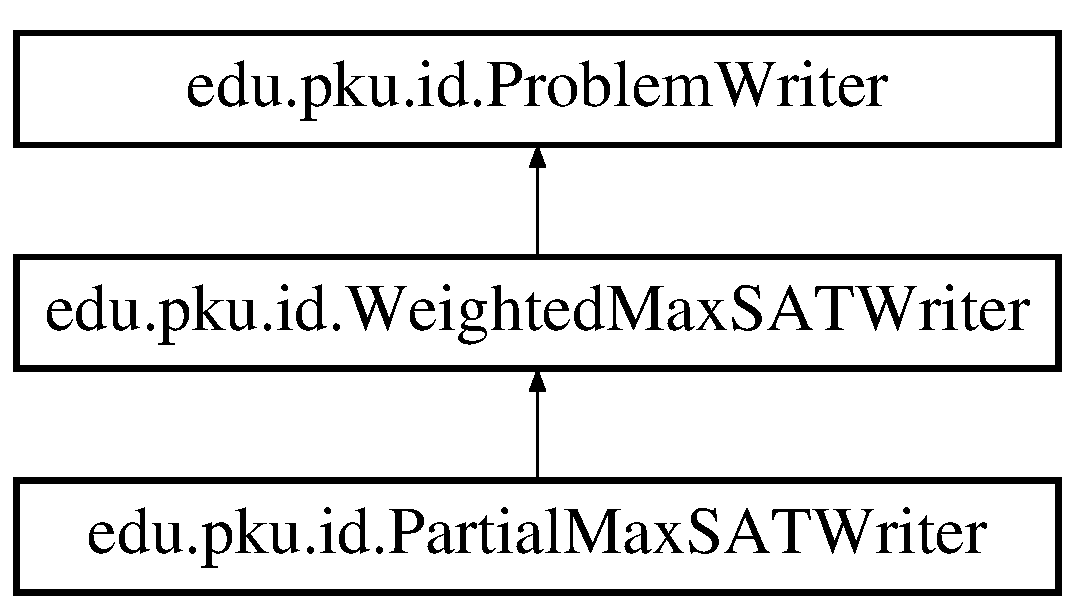
\includegraphics[height=3.000000cm]{classedu_1_1pku_1_1id_1_1_weighted_max_s_a_t_writer}
\end{center}
\end{figure}
\subsection*{Public Member Functions}
\begin{DoxyCompactItemize}
\item 
\hyperlink{classedu_1_1pku_1_1id_1_1_weighted_max_s_a_t_writer_a384ae98af244daa4374615d25ede7f87}{WeightedMaxSATWriter} (List$<$ \hyperlink{classedu_1_1pku_1_1id_1_1_weighted_clause}{WeightedClause} $>$ \hyperlink{classedu_1_1pku_1_1id_1_1_weighted_max_s_a_t_writer_a73dc99c36bfbaf938f3ffb7b95189d37}{weightedClauses}, int \hyperlink{classedu_1_1pku_1_1id_1_1_weighted_max_s_a_t_writer_ae9c3e5d651a1b8100fd5d85f00a18a54}{nbVars}, String fileName)  throws IOException 
\item 
void \hyperlink{classedu_1_1pku_1_1id_1_1_weighted_max_s_a_t_writer_a9ca988f376b3618c2b6b4724feb6a9f5}{write} ()  throws IOException 
\end{DoxyCompactItemize}
\subsection*{Protected Member Functions}
\begin{DoxyCompactItemize}
\item 
void \hyperlink{classedu_1_1pku_1_1id_1_1_weighted_max_s_a_t_writer_af39eb87193ec92810ed0cfcef4a4a626}{writeProblem} ()  throws IOException 
\end{DoxyCompactItemize}
\subsection*{Protected Attributes}
\begin{DoxyCompactItemize}
\item 
List$<$ \hyperlink{classedu_1_1pku_1_1id_1_1_weighted_clause}{WeightedClause} $>$ \hyperlink{classedu_1_1pku_1_1id_1_1_weighted_max_s_a_t_writer_a73dc99c36bfbaf938f3ffb7b95189d37}{weightedClauses}
\item 
int \hyperlink{classedu_1_1pku_1_1id_1_1_weighted_max_s_a_t_writer_ae9c3e5d651a1b8100fd5d85f00a18a54}{nbVars}
\end{DoxyCompactItemize}
\subsection*{Package Attributes}
\begin{DoxyCompactItemize}
\item 
FileWriter \hyperlink{classedu_1_1pku_1_1id_1_1_weighted_max_s_a_t_writer_a6804c608ef104e3ee760359325c9fd55}{writer}
\end{DoxyCompactItemize}
\subsection*{Private Member Functions}
\begin{DoxyCompactItemize}
\item 
void \hyperlink{classedu_1_1pku_1_1id_1_1_weighted_max_s_a_t_writer_aee8f85aa6cf3ef30a1b2a1f1a69585bc}{writeWeightedClauses} ()  throws IOException 
\item 
void \hyperlink{classedu_1_1pku_1_1id_1_1_weighted_max_s_a_t_writer_acdb3644a2754695c63b536a466787a24}{writeWeightedClause} (\hyperlink{classedu_1_1pku_1_1id_1_1_weighted_clause}{WeightedClause} weightedClause)  throws IOException 
\item 
void \hyperlink{classedu_1_1pku_1_1id_1_1_weighted_max_s_a_t_writer_a466550c5948e4d6e453be69374858568}{writeHeader} ()  throws IOException 
\end{DoxyCompactItemize}


\subsection{Constructor \& Destructor Documentation}
\hypertarget{classedu_1_1pku_1_1id_1_1_weighted_max_s_a_t_writer_a384ae98af244daa4374615d25ede7f87}{
\index{edu::pku::id::WeightedMaxSATWriter@{edu::pku::id::WeightedMaxSATWriter}!WeightedMaxSATWriter@{WeightedMaxSATWriter}}
\index{WeightedMaxSATWriter@{WeightedMaxSATWriter}!edu::pku::id::WeightedMaxSATWriter@{edu::pku::id::WeightedMaxSATWriter}}
\subsubsection[{WeightedMaxSATWriter}]{\setlength{\rightskip}{0pt plus 5cm}edu.pku.id.WeightedMaxSATWriter.WeightedMaxSATWriter (
\begin{DoxyParamCaption}
\item[{List$<$ {\bf WeightedClause} $>$}]{ weightedClauses, }
\item[{int}]{ nbVars, }
\item[{String}]{ fileName}
\end{DoxyParamCaption}
)  throws IOException }}
\label{classedu_1_1pku_1_1id_1_1_weighted_max_s_a_t_writer_a384ae98af244daa4374615d25ede7f87}


\subsection{Member Function Documentation}
\hypertarget{classedu_1_1pku_1_1id_1_1_weighted_max_s_a_t_writer_a9ca988f376b3618c2b6b4724feb6a9f5}{
\index{edu::pku::id::WeightedMaxSATWriter@{edu::pku::id::WeightedMaxSATWriter}!write@{write}}
\index{write@{write}!edu::pku::id::WeightedMaxSATWriter@{edu::pku::id::WeightedMaxSATWriter}}
\subsubsection[{write}]{\setlength{\rightskip}{0pt plus 5cm}void edu.pku.id.WeightedMaxSATWriter.write (
\begin{DoxyParamCaption}
{}
\end{DoxyParamCaption}
)  throws IOException \hspace{0.3cm}{\ttfamily  \mbox{[}virtual\mbox{]}}}}
\label{classedu_1_1pku_1_1id_1_1_weighted_max_s_a_t_writer_a9ca988f376b3618c2b6b4724feb6a9f5}


Implements \hyperlink{interfaceedu_1_1pku_1_1id_1_1_problem_writer_aa2c5df4e6546cb6d7980d179cc8f91cd}{edu.pku.id.ProblemWriter}.

\hypertarget{classedu_1_1pku_1_1id_1_1_weighted_max_s_a_t_writer_a466550c5948e4d6e453be69374858568}{
\index{edu::pku::id::WeightedMaxSATWriter@{edu::pku::id::WeightedMaxSATWriter}!writeHeader@{writeHeader}}
\index{writeHeader@{writeHeader}!edu::pku::id::WeightedMaxSATWriter@{edu::pku::id::WeightedMaxSATWriter}}
\subsubsection[{writeHeader}]{\setlength{\rightskip}{0pt plus 5cm}void edu.pku.id.WeightedMaxSATWriter.writeHeader (
\begin{DoxyParamCaption}
{}
\end{DoxyParamCaption}
)  throws IOException \hspace{0.3cm}{\ttfamily  \mbox{[}private\mbox{]}}}}
\label{classedu_1_1pku_1_1id_1_1_weighted_max_s_a_t_writer_a466550c5948e4d6e453be69374858568}
\hypertarget{classedu_1_1pku_1_1id_1_1_weighted_max_s_a_t_writer_af39eb87193ec92810ed0cfcef4a4a626}{
\index{edu::pku::id::WeightedMaxSATWriter@{edu::pku::id::WeightedMaxSATWriter}!writeProblem@{writeProblem}}
\index{writeProblem@{writeProblem}!edu::pku::id::WeightedMaxSATWriter@{edu::pku::id::WeightedMaxSATWriter}}
\subsubsection[{writeProblem}]{\setlength{\rightskip}{0pt plus 5cm}void edu.pku.id.WeightedMaxSATWriter.writeProblem (
\begin{DoxyParamCaption}
{}
\end{DoxyParamCaption}
)  throws IOException \hspace{0.3cm}{\ttfamily  \mbox{[}protected\mbox{]}}}}
\label{classedu_1_1pku_1_1id_1_1_weighted_max_s_a_t_writer_af39eb87193ec92810ed0cfcef4a4a626}


Reimplemented in \hyperlink{classedu_1_1pku_1_1id_1_1_partial_max_s_a_t_writer_ab066f4e7f38654fefdeb3cc02b56026f}{edu.pku.id.PartialMaxSATWriter}.

\hypertarget{classedu_1_1pku_1_1id_1_1_weighted_max_s_a_t_writer_acdb3644a2754695c63b536a466787a24}{
\index{edu::pku::id::WeightedMaxSATWriter@{edu::pku::id::WeightedMaxSATWriter}!writeWeightedClause@{writeWeightedClause}}
\index{writeWeightedClause@{writeWeightedClause}!edu::pku::id::WeightedMaxSATWriter@{edu::pku::id::WeightedMaxSATWriter}}
\subsubsection[{writeWeightedClause}]{\setlength{\rightskip}{0pt plus 5cm}void edu.pku.id.WeightedMaxSATWriter.writeWeightedClause (
\begin{DoxyParamCaption}
\item[{{\bf WeightedClause}}]{ weightedClause}
\end{DoxyParamCaption}
)  throws IOException \hspace{0.3cm}{\ttfamily  \mbox{[}private\mbox{]}}}}
\label{classedu_1_1pku_1_1id_1_1_weighted_max_s_a_t_writer_acdb3644a2754695c63b536a466787a24}
\hypertarget{classedu_1_1pku_1_1id_1_1_weighted_max_s_a_t_writer_aee8f85aa6cf3ef30a1b2a1f1a69585bc}{
\index{edu::pku::id::WeightedMaxSATWriter@{edu::pku::id::WeightedMaxSATWriter}!writeWeightedClauses@{writeWeightedClauses}}
\index{writeWeightedClauses@{writeWeightedClauses}!edu::pku::id::WeightedMaxSATWriter@{edu::pku::id::WeightedMaxSATWriter}}
\subsubsection[{writeWeightedClauses}]{\setlength{\rightskip}{0pt plus 5cm}void edu.pku.id.WeightedMaxSATWriter.writeWeightedClauses (
\begin{DoxyParamCaption}
{}
\end{DoxyParamCaption}
)  throws IOException \hspace{0.3cm}{\ttfamily  \mbox{[}private\mbox{]}}}}
\label{classedu_1_1pku_1_1id_1_1_weighted_max_s_a_t_writer_aee8f85aa6cf3ef30a1b2a1f1a69585bc}


\subsection{Member Data Documentation}
\hypertarget{classedu_1_1pku_1_1id_1_1_weighted_max_s_a_t_writer_ae9c3e5d651a1b8100fd5d85f00a18a54}{
\index{edu::pku::id::WeightedMaxSATWriter@{edu::pku::id::WeightedMaxSATWriter}!nbVars@{nbVars}}
\index{nbVars@{nbVars}!edu::pku::id::WeightedMaxSATWriter@{edu::pku::id::WeightedMaxSATWriter}}
\subsubsection[{nbVars}]{\setlength{\rightskip}{0pt plus 5cm}int {\bf edu.pku.id.WeightedMaxSATWriter.nbVars}\hspace{0.3cm}{\ttfamily  \mbox{[}protected\mbox{]}}}}
\label{classedu_1_1pku_1_1id_1_1_weighted_max_s_a_t_writer_ae9c3e5d651a1b8100fd5d85f00a18a54}
\hypertarget{classedu_1_1pku_1_1id_1_1_weighted_max_s_a_t_writer_a73dc99c36bfbaf938f3ffb7b95189d37}{
\index{edu::pku::id::WeightedMaxSATWriter@{edu::pku::id::WeightedMaxSATWriter}!weightedClauses@{weightedClauses}}
\index{weightedClauses@{weightedClauses}!edu::pku::id::WeightedMaxSATWriter@{edu::pku::id::WeightedMaxSATWriter}}
\subsubsection[{weightedClauses}]{\setlength{\rightskip}{0pt plus 5cm}List$<${\bf WeightedClause}$>$ {\bf edu.pku.id.WeightedMaxSATWriter.weightedClauses}\hspace{0.3cm}{\ttfamily  \mbox{[}protected\mbox{]}}}}
\label{classedu_1_1pku_1_1id_1_1_weighted_max_s_a_t_writer_a73dc99c36bfbaf938f3ffb7b95189d37}
\hypertarget{classedu_1_1pku_1_1id_1_1_weighted_max_s_a_t_writer_a6804c608ef104e3ee760359325c9fd55}{
\index{edu::pku::id::WeightedMaxSATWriter@{edu::pku::id::WeightedMaxSATWriter}!writer@{writer}}
\index{writer@{writer}!edu::pku::id::WeightedMaxSATWriter@{edu::pku::id::WeightedMaxSATWriter}}
\subsubsection[{writer}]{\setlength{\rightskip}{0pt plus 5cm}FileWriter {\bf edu.pku.id.WeightedMaxSATWriter.writer}\hspace{0.3cm}{\ttfamily  \mbox{[}package\mbox{]}}}}
\label{classedu_1_1pku_1_1id_1_1_weighted_max_s_a_t_writer_a6804c608ef104e3ee760359325c9fd55}


The documentation for this class was generated from the following file:\begin{DoxyCompactItemize}
\item 
src/edu/pku/id/\hyperlink{_weighted_max_s_a_t_writer_8java}{WeightedMaxSATWriter.java}\end{DoxyCompactItemize}

\chapter{File Documentation}
\hypertarget{_inc_degree_encoder_cli_8java}{
\section{src/edu/pku/id/cli/IncDegreeEncoderCli.java File Reference}
\label{_inc_degree_encoder_cli_8java}\index{src/edu/pku/id/cli/IncDegreeEncoderCli.java@{src/edu/pku/id/cli/IncDegreeEncoderCli.java}}
}
\subsection*{Classes}
\begin{DoxyCompactItemize}
\item 
class \hyperlink{classedu_1_1pku_1_1id_1_1cli_1_1_inc_degree_encoder_cli}{edu.pku.id.cli.IncDegreeEncoderCli}
\end{DoxyCompactItemize}
\subsection*{Packages}
\begin{DoxyCompactItemize}
\item 
package \hyperlink{namespaceedu_1_1pku_1_1id_1_1cli}{edu.pku.id.cli}
\end{DoxyCompactItemize}

\hypertarget{_multi_valued_translater_cli_8java}{
\section{src/edu/pku/id/cli/MultiValuedTranslaterCli.java File Reference}
\label{_multi_valued_translater_cli_8java}\index{src/edu/pku/id/cli/MultiValuedTranslaterCli.java@{src/edu/pku/id/cli/MultiValuedTranslaterCli.java}}
}
\subsection*{Classes}
\begin{DoxyCompactItemize}
\item 
class \hyperlink{classedu_1_1pku_1_1id_1_1cli_1_1_multi_valued_translater_cli}{edu.pku.id.cli.MultiValuedTranslaterCli}
\end{DoxyCompactItemize}
\subsection*{Packages}
\begin{DoxyCompactItemize}
\item 
package \hyperlink{namespaceedu_1_1pku_1_1id_1_1cli}{edu.pku.id.cli}
\end{DoxyCompactItemize}

\hypertarget{_result_model_reader_8java}{
\section{src/edu/pku/id/cli/ResultModelReader.java File Reference}
\label{_result_model_reader_8java}\index{src/edu/pku/id/cli/ResultModelReader.java@{src/edu/pku/id/cli/ResultModelReader.java}}
}
\subsection*{Classes}
\begin{DoxyCompactItemize}
\item 
class \hyperlink{classedu_1_1pku_1_1id_1_1cli_1_1_result_model_reader}{edu.pku.id.cli.ResultModelReader}
\end{DoxyCompactItemize}
\subsection*{Packages}
\begin{DoxyCompactItemize}
\item 
package \hyperlink{namespaceedu_1_1pku_1_1id_1_1cli}{edu.pku.id.cli}
\end{DoxyCompactItemize}

\hypertarget{_cnf_file_q_c_translater_8java}{
\section{src/edu/pku/id/CnfFileQCTranslater.java File Reference}
\label{_cnf_file_q_c_translater_8java}\index{src/edu/pku/id/CnfFileQCTranslater.java@{src/edu/pku/id/CnfFileQCTranslater.java}}
}
\subsection*{Classes}
\begin{DoxyCompactItemize}
\item 
class \hyperlink{classedu_1_1pku_1_1id_1_1_cnf_file_q_c_translater}{edu.pku.id.CnfFileQCTranslater}
\end{DoxyCompactItemize}
\subsection*{Packages}
\begin{DoxyCompactItemize}
\item 
package \hyperlink{namespaceedu_1_1pku_1_1id}{edu.pku.id}
\end{DoxyCompactItemize}

\hypertarget{_cnf_file_reader_8java}{
\section{src/edu/pku/id/CnfFileReader.java File Reference}
\label{_cnf_file_reader_8java}\index{src/edu/pku/id/CnfFileReader.java@{src/edu/pku/id/CnfFileReader.java}}
}
\subsection*{Classes}
\begin{DoxyCompactItemize}
\item 
class \hyperlink{classedu_1_1pku_1_1id_1_1_cnf_file_reader}{edu.pku.id.CnfFileReader}
\end{DoxyCompactItemize}
\subsection*{Packages}
\begin{DoxyCompactItemize}
\item 
package \hyperlink{namespaceedu_1_1pku_1_1id}{edu.pku.id}
\end{DoxyCompactItemize}

\hypertarget{_m_u_s_file_reader_8java}{
\section{src/edu/pku/id/file/MUSFileReader.java File Reference}
\label{_m_u_s_file_reader_8java}\index{src/edu/pku/id/file/MUSFileReader.java@{src/edu/pku/id/file/MUSFileReader.java}}
}
\subsection*{Classes}
\begin{DoxyCompactItemize}
\item 
class \hyperlink{classedu_1_1pku_1_1id_1_1file_1_1_m_u_s_file_reader}{edu.pku.id.file.MUSFileReader}
\end{DoxyCompactItemize}
\subsection*{Packages}
\begin{DoxyCompactItemize}
\item 
package \hyperlink{namespaceedu_1_1pku_1_1id_1_1file}{edu.pku.id.file}
\end{DoxyCompactItemize}

\hypertarget{_four_valued_translater_8java}{
\section{src/edu/pku/id/FourValuedTranslater.java File Reference}
\label{_four_valued_translater_8java}\index{src/edu/pku/id/FourValuedTranslater.java@{src/edu/pku/id/FourValuedTranslater.java}}
}
\subsection*{Classes}
\begin{DoxyCompactItemize}
\item 
class \hyperlink{classedu_1_1pku_1_1id_1_1_four_valued_translater}{edu.pku.id.FourValuedTranslater}
\end{DoxyCompactItemize}
\subsection*{Packages}
\begin{DoxyCompactItemize}
\item 
package \hyperlink{namespaceedu_1_1pku_1_1id}{edu.pku.id}
\end{DoxyCompactItemize}

\hypertarget{_i_d_measurer_8java}{
\section{src/edu/pku/id/IDMeasurer.java File Reference}
\label{_i_d_measurer_8java}\index{src/edu/pku/id/IDMeasurer.java@{src/edu/pku/id/IDMeasurer.java}}
}
\subsection*{Classes}
\begin{DoxyCompactItemize}
\item 
class \hyperlink{classedu_1_1pku_1_1id_1_1_i_d_measurer}{edu.pku.id.IDMeasurer}
\end{DoxyCompactItemize}
\subsection*{Packages}
\begin{DoxyCompactItemize}
\item 
package \hyperlink{namespaceedu_1_1pku_1_1id}{edu.pku.id}
\end{DoxyCompactItemize}

\hypertarget{_inconsistency_degree_encoder_8java}{
\section{src/edu/pku/id/InconsistencyDegreeEncoder.java File Reference}
\label{_inconsistency_degree_encoder_8java}\index{src/edu/pku/id/InconsistencyDegreeEncoder.java@{src/edu/pku/id/InconsistencyDegreeEncoder.java}}
}
\subsection*{Classes}
\begin{DoxyCompactItemize}
\item 
class \hyperlink{classedu_1_1pku_1_1id_1_1_inconsistency_degree_encoder}{edu.pku.id.InconsistencyDegreeEncoder}
\end{DoxyCompactItemize}
\subsection*{Packages}
\begin{DoxyCompactItemize}
\item 
package \hyperlink{namespaceedu_1_1pku_1_1id}{edu.pku.id}
\end{DoxyCompactItemize}

\hypertarget{_i_q_c_reasoner_8java}{
\section{src/edu/pku/id/IQCReasoner.java File Reference}
\label{_i_q_c_reasoner_8java}\index{src/edu/pku/id/IQCReasoner.java@{src/edu/pku/id/IQCReasoner.java}}
}
\subsection*{Classes}
\begin{DoxyCompactItemize}
\item 
interface \hyperlink{interfaceedu_1_1pku_1_1id_1_1_i_q_c_reasoner}{edu.pku.id.IQCReasoner}
\end{DoxyCompactItemize}
\subsection*{Packages}
\begin{DoxyCompactItemize}
\item 
package \hyperlink{namespaceedu_1_1pku_1_1id}{edu.pku.id}
\end{DoxyCompactItemize}

\hypertarget{_multi_valued_semantics_8java}{
\section{src/edu/pku/id/MultiValuedSemantics.java File Reference}
\label{_multi_valued_semantics_8java}\index{src/edu/pku/id/MultiValuedSemantics.java@{src/edu/pku/id/MultiValuedSemantics.java}}
}
\subsection*{Packages}
\begin{DoxyCompactItemize}
\item 
package \hyperlink{namespaceedu_1_1pku_1_1id}{edu.pku.id}
\end{DoxyCompactItemize}
\subsection*{Enumerations}
\begin{DoxyCompactItemize}
\item 
enum \hyperlink{namespaceedu_1_1pku_1_1id_ad71ddcb0be4b31cdeeb2a5d755309f2d}{edu::pku::id.MultiValuedSemantics} \{ \hyperlink{namespaceedu_1_1pku_1_1id_ad71ddcb0be4b31cdeeb2a5d755309f2d}{edu::pku::id.Four}, 
\hyperlink{namespaceedu_1_1pku_1_1id_ad71ddcb0be4b31cdeeb2a5d755309f2d}{edu::pku::id.QC}, 
\hyperlink{namespaceedu_1_1pku_1_1id_ad71ddcb0be4b31cdeeb2a5d755309f2d}{edu::pku::id.LPm}, 
\hyperlink{namespaceedu_1_1pku_1_1id_ad71ddcb0be4b31cdeeb2a5d755309f2d}{edu::pku::id.Three}
 \}
\end{DoxyCompactItemize}

\hypertarget{_multi_valued_translater_8java}{
\section{src/edu/pku/id/MultiValuedTranslater.java File Reference}
\label{_multi_valued_translater_8java}\index{src/edu/pku/id/MultiValuedTranslater.java@{src/edu/pku/id/MultiValuedTranslater.java}}
}
\subsection*{Classes}
\begin{DoxyCompactItemize}
\item 
class \hyperlink{classedu_1_1pku_1_1id_1_1_multi_valued_translater}{edu.pku.id.MultiValuedTranslater}
\end{DoxyCompactItemize}
\subsection*{Packages}
\begin{DoxyCompactItemize}
\item 
package \hyperlink{namespaceedu_1_1pku_1_1id}{edu.pku.id}
\end{DoxyCompactItemize}

\hypertarget{_i_d_q___m_u_s_8java}{
\section{src/edu/pku/id/mus/IDQ\_\-MUS.java File Reference}
\label{_i_d_q___m_u_s_8java}\index{src/edu/pku/id/mus/IDQ\_\-MUS.java@{src/edu/pku/id/mus/IDQ\_\-MUS.java}}
}
\subsection*{Classes}
\begin{DoxyCompactItemize}
\item 
class \hyperlink{classedu_1_1pku_1_1id_1_1mus_1_1_i_d_q___m_u_s}{edu.pku.id.mus.IDQ\_\-MUS}
\end{DoxyCompactItemize}
\subsection*{Packages}
\begin{DoxyCompactItemize}
\item 
package \hyperlink{namespaceedu_1_1pku_1_1id_1_1mus}{edu.pku.id.mus}
\end{DoxyCompactItemize}

\hypertarget{_i_d_q_measurer___p_b_8java}{
\section{src/edu/pku/id/mus/IDQMeasurer\_\-PB.java File Reference}
\label{_i_d_q_measurer___p_b_8java}\index{src/edu/pku/id/mus/IDQMeasurer\_\-PB.java@{src/edu/pku/id/mus/IDQMeasurer\_\-PB.java}}
}
\subsection*{Classes}
\begin{DoxyCompactItemize}
\item 
class \hyperlink{classedu_1_1pku_1_1id_1_1mus_1_1_i_d_q_measurer___p_b}{edu.pku.id.mus.IDQMeasurer\_\-PB}
\end{DoxyCompactItemize}
\subsection*{Packages}
\begin{DoxyCompactItemize}
\item 
package \hyperlink{namespaceedu_1_1pku_1_1id_1_1mus}{edu.pku.id.mus}
\end{DoxyCompactItemize}

\hypertarget{_p_b_constraint_8java}{
\section{src/edu/pku/id/mus/PBConstraint.java File Reference}
\label{_p_b_constraint_8java}\index{src/edu/pku/id/mus/PBConstraint.java@{src/edu/pku/id/mus/PBConstraint.java}}
}
\subsection*{Classes}
\begin{DoxyCompactItemize}
\item 
class \hyperlink{classedu_1_1pku_1_1id_1_1mus_1_1_p_b_constraint}{edu.pku.id.mus.PBConstraint}
\end{DoxyCompactItemize}
\subsection*{Packages}
\begin{DoxyCompactItemize}
\item 
package \hyperlink{namespaceedu_1_1pku_1_1id_1_1mus}{edu.pku.id.mus}
\end{DoxyCompactItemize}

\hypertarget{_p_b_term_8java}{
\section{src/edu/pku/id/mus/PBTerm.java File Reference}
\label{_p_b_term_8java}\index{src/edu/pku/id/mus/PBTerm.java@{src/edu/pku/id/mus/PBTerm.java}}
}
\subsection*{Classes}
\begin{DoxyCompactItemize}
\item 
class \hyperlink{classedu_1_1pku_1_1id_1_1mus_1_1_p_b_term}{edu.pku.id.mus.PBTerm}
\end{DoxyCompactItemize}
\subsection*{Packages}
\begin{DoxyCompactItemize}
\item 
package \hyperlink{namespaceedu_1_1pku_1_1id_1_1mus}{edu.pku.id.mus}
\end{DoxyCompactItemize}

\hypertarget{_s_a_t2_p_b_translater___q_c_8java}{
\section{src/edu/pku/id/mus/SAT2PBTranslater\_\-QC.java File Reference}
\label{_s_a_t2_p_b_translater___q_c_8java}\index{src/edu/pku/id/mus/SAT2PBTranslater\_\-QC.java@{src/edu/pku/id/mus/SAT2PBTranslater\_\-QC.java}}
}
\subsection*{Classes}
\begin{DoxyCompactItemize}
\item 
class \hyperlink{classedu_1_1pku_1_1id_1_1mus_1_1_s_a_t2_p_b_translater___q_c}{edu.pku.id.mus.SAT2PBTranslater\_\-QC}
\end{DoxyCompactItemize}
\subsection*{Packages}
\begin{DoxyCompactItemize}
\item 
package \hyperlink{namespaceedu_1_1pku_1_1id_1_1mus}{edu.pku.id.mus}
\end{DoxyCompactItemize}

\hypertarget{_partial_max_s_a_t_writer_8java}{
\section{src/edu/pku/id/PartialMaxSATWriter.java File Reference}
\label{_partial_max_s_a_t_writer_8java}\index{src/edu/pku/id/PartialMaxSATWriter.java@{src/edu/pku/id/PartialMaxSATWriter.java}}
}
\subsection*{Classes}
\begin{DoxyCompactItemize}
\item 
class \hyperlink{classedu_1_1pku_1_1id_1_1_partial_max_s_a_t_writer}{edu.pku.id.PartialMaxSATWriter}
\end{DoxyCompactItemize}
\subsection*{Packages}
\begin{DoxyCompactItemize}
\item 
package \hyperlink{namespaceedu_1_1pku_1_1id}{edu.pku.id}
\end{DoxyCompactItemize}

\hypertarget{_p_b_report_8java}{
\section{src/edu/pku/id/pbsolver/PBReport.java File Reference}
\label{_p_b_report_8java}\index{src/edu/pku/id/pbsolver/PBReport.java@{src/edu/pku/id/pbsolver/PBReport.java}}
}
\subsection*{Classes}
\begin{DoxyCompactItemize}
\item 
class \hyperlink{classedu_1_1pku_1_1id_1_1pbsolver_1_1_p_b_report}{edu.pku.id.pbsolver.PBReport}
\end{DoxyCompactItemize}
\subsection*{Packages}
\begin{DoxyCompactItemize}
\item 
package \hyperlink{namespaceedu_1_1pku_1_1id_1_1pbsolver}{edu.pku.id.pbsolver}
\end{DoxyCompactItemize}

\hypertarget{_p_b_solver_8java}{
\section{src/edu/pku/id/pbsolver/PBSolver.java File Reference}
\label{_p_b_solver_8java}\index{src/edu/pku/id/pbsolver/PBSolver.java@{src/edu/pku/id/pbsolver/PBSolver.java}}
}
\subsection*{Classes}
\begin{DoxyCompactItemize}
\item 
class \hyperlink{classedu_1_1pku_1_1id_1_1pbsolver_1_1_p_b_solver}{edu.pku.id.pbsolver.PBSolver}
\end{DoxyCompactItemize}
\subsection*{Packages}
\begin{DoxyCompactItemize}
\item 
package \hyperlink{namespaceedu_1_1pku_1_1id_1_1pbsolver}{edu.pku.id.pbsolver}
\end{DoxyCompactItemize}

\hypertarget{_problem_generator_8java}{
\section{src/edu/pku/id/ProblemGenerator.java File Reference}
\label{_problem_generator_8java}\index{src/edu/pku/id/ProblemGenerator.java@{src/edu/pku/id/ProblemGenerator.java}}
}
\subsection*{Classes}
\begin{DoxyCompactItemize}
\item 
class \hyperlink{classedu_1_1pku_1_1id_1_1_problem_generator}{edu.pku.id.ProblemGenerator}
\end{DoxyCompactItemize}
\subsection*{Packages}
\begin{DoxyCompactItemize}
\item 
package \hyperlink{namespaceedu_1_1pku_1_1id}{edu.pku.id}
\end{DoxyCompactItemize}

\hypertarget{_problem_writer_8java}{
\section{src/edu/pku/id/ProblemWriter.java File Reference}
\label{_problem_writer_8java}\index{src/edu/pku/id/ProblemWriter.java@{src/edu/pku/id/ProblemWriter.java}}
}
\subsection*{Classes}
\begin{DoxyCompactItemize}
\item 
interface \hyperlink{interfaceedu_1_1pku_1_1id_1_1_problem_writer}{edu.pku.id.ProblemWriter}
\end{DoxyCompactItemize}
\subsection*{Packages}
\begin{DoxyCompactItemize}
\item 
package \hyperlink{namespaceedu_1_1pku_1_1id}{edu.pku.id}
\end{DoxyCompactItemize}

\hypertarget{_q_c_reasoner_8java}{
\section{src/edu/pku/id/QCReasoner.java File Reference}
\label{_q_c_reasoner_8java}\index{src/edu/pku/id/QCReasoner.java@{src/edu/pku/id/QCReasoner.java}}
}
\subsection*{Classes}
\begin{DoxyCompactItemize}
\item 
class \hyperlink{classedu_1_1pku_1_1id_1_1_q_c_reasoner}{edu.pku.id.QCReasoner}
\end{DoxyCompactItemize}
\subsection*{Packages}
\begin{DoxyCompactItemize}
\item 
package \hyperlink{namespaceedu_1_1pku_1_1id}{edu.pku.id}
\end{DoxyCompactItemize}

\hypertarget{_q_c_reasoner_v2_8java}{
\section{src/edu/pku/id/QCReasonerV2.java File Reference}
\label{_q_c_reasoner_v2_8java}\index{src/edu/pku/id/QCReasonerV2.java@{src/edu/pku/id/QCReasonerV2.java}}
}
\subsection*{Classes}
\begin{DoxyCompactItemize}
\item 
class \hyperlink{classedu_1_1pku_1_1id_1_1_q_c_reasoner_v2}{edu.pku.id.QCReasonerV2}
\end{DoxyCompactItemize}
\subsection*{Packages}
\begin{DoxyCompactItemize}
\item 
package \hyperlink{namespaceedu_1_1pku_1_1id}{edu.pku.id}
\end{DoxyCompactItemize}

\hypertarget{_q_c_translater_8java}{
\section{src/edu/pku/id/QCTranslater.java File Reference}
\label{_q_c_translater_8java}\index{src/edu/pku/id/QCTranslater.java@{src/edu/pku/id/QCTranslater.java}}
}
\subsection*{Classes}
\begin{DoxyCompactItemize}
\item 
class \hyperlink{classedu_1_1pku_1_1id_1_1_q_c_translater}{edu.pku.id.QCTranslater}
\end{DoxyCompactItemize}
\subsection*{Packages}
\begin{DoxyCompactItemize}
\item 
package \hyperlink{namespaceedu_1_1pku_1_1id}{edu.pku.id}
\end{DoxyCompactItemize}

\hypertarget{_s_a_t_problem_type_8java}{
\section{src/edu/pku/id/SATProblemType.java File Reference}
\label{_s_a_t_problem_type_8java}\index{src/edu/pku/id/SATProblemType.java@{src/edu/pku/id/SATProblemType.java}}
}
\subsection*{Packages}
\begin{DoxyCompactItemize}
\item 
package \hyperlink{namespaceedu_1_1pku_1_1id}{edu.pku.id}
\end{DoxyCompactItemize}
\subsection*{Enumerations}
\begin{DoxyCompactItemize}
\item 
enum \hyperlink{namespaceedu_1_1pku_1_1id_a7936f4efdc70b70b965d63bd005a2513}{edu::pku::id.SATProblemType} \{ \hyperlink{namespaceedu_1_1pku_1_1id_a7936f4efdc70b70b965d63bd005a2513}{edu::pku::id.SAT}, 
\hyperlink{namespaceedu_1_1pku_1_1id_a7936f4efdc70b70b965d63bd005a2513}{edu::pku::id.MaxSAT}, 
\hyperlink{namespaceedu_1_1pku_1_1id_a7936f4efdc70b70b965d63bd005a2513}{edu::pku::id.PartialMaxSAT}, 
\hyperlink{namespaceedu_1_1pku_1_1id_a7936f4efdc70b70b965d63bd005a2513}{edu::pku::id.WeightedMaxSAT}
 \}
\end{DoxyCompactItemize}

\hypertarget{_truth_value_8java}{
\section{src/edu/pku/id/TruthValue.java File Reference}
\label{_truth_value_8java}\index{src/edu/pku/id/TruthValue.java@{src/edu/pku/id/TruthValue.java}}
}
\subsection*{Packages}
\begin{DoxyCompactItemize}
\item 
package \hyperlink{namespaceedu_1_1pku_1_1id}{edu.pku.id}
\end{DoxyCompactItemize}
\subsection*{Enumerations}
\begin{DoxyCompactItemize}
\item 
enum \hyperlink{namespaceedu_1_1pku_1_1id_a01cdd35063021f272bd905de5f43f634}{edu::pku::id.TruthValue} \{ \hyperlink{namespaceedu_1_1pku_1_1id_a01cdd35063021f272bd905de5f43f634}{edu::pku::id.True}, 
\hyperlink{namespaceedu_1_1pku_1_1id_a01cdd35063021f272bd905de5f43f634}{edu::pku::id.False}, 
\hyperlink{namespaceedu_1_1pku_1_1id_a01cdd35063021f272bd905de5f43f634}{edu::pku::id.Both}, 
\hyperlink{namespaceedu_1_1pku_1_1id_a01cdd35063021f272bd905de5f43f634}{edu::pku::id.None}
 \}
\end{DoxyCompactItemize}

\hypertarget{_wcnf_file_reader_8java}{
\section{src/edu/pku/id/WcnfFileReader.java File Reference}
\label{_wcnf_file_reader_8java}\index{src/edu/pku/id/WcnfFileReader.java@{src/edu/pku/id/WcnfFileReader.java}}
}
\subsection*{Classes}
\begin{DoxyCompactItemize}
\item 
class \hyperlink{classedu_1_1pku_1_1id_1_1_wcnf_file_reader}{edu.pku.id.WcnfFileReader}
\end{DoxyCompactItemize}
\subsection*{Packages}
\begin{DoxyCompactItemize}
\item 
package \hyperlink{namespaceedu_1_1pku_1_1id}{edu.pku.id}
\end{DoxyCompactItemize}

\hypertarget{_weighted_clause_8java}{
\section{src/edu/pku/id/WeightedClause.java File Reference}
\label{_weighted_clause_8java}\index{src/edu/pku/id/WeightedClause.java@{src/edu/pku/id/WeightedClause.java}}
}
\subsection*{Classes}
\begin{DoxyCompactItemize}
\item 
class \hyperlink{classedu_1_1pku_1_1id_1_1_weighted_clause}{edu.pku.id.WeightedClause}
\end{DoxyCompactItemize}
\subsection*{Packages}
\begin{DoxyCompactItemize}
\item 
package \hyperlink{namespaceedu_1_1pku_1_1id}{edu.pku.id}
\end{DoxyCompactItemize}

\hypertarget{_weighted_max_s_a_t_writer_8java}{
\section{src/edu/pku/id/WeightedMaxSATWriter.java File Reference}
\label{_weighted_max_s_a_t_writer_8java}\index{src/edu/pku/id/WeightedMaxSATWriter.java@{src/edu/pku/id/WeightedMaxSATWriter.java}}
}
\subsection*{Classes}
\begin{DoxyCompactItemize}
\item 
class \hyperlink{classedu_1_1pku_1_1id_1_1_weighted_max_s_a_t_writer}{edu.pku.id.WeightedMaxSATWriter}
\end{DoxyCompactItemize}
\subsection*{Packages}
\begin{DoxyCompactItemize}
\item 
package \hyperlink{namespaceedu_1_1pku_1_1id}{edu.pku.id}
\end{DoxyCompactItemize}

\hypertarget{_getopt_8java}{
\section{src/gnu/getopt/Getopt.java File Reference}
\label{_getopt_8java}\index{src/gnu/getopt/Getopt.java@{src/gnu/getopt/Getopt.java}}
}
\subsection*{Classes}
\begin{DoxyCompactItemize}
\item 
class \hyperlink{classgnu_1_1getopt_1_1_getopt}{gnu.getopt.Getopt}
\end{DoxyCompactItemize}
\subsection*{Packages}
\begin{DoxyCompactItemize}
\item 
package \hyperlink{namespacegnu_1_1getopt}{gnu.getopt}
\end{DoxyCompactItemize}

\hypertarget{_long_opt_8java}{
\section{src/gnu/getopt/LongOpt.java File Reference}
\label{_long_opt_8java}\index{src/gnu/getopt/LongOpt.java@{src/gnu/getopt/LongOpt.java}}
}
\subsection*{Classes}
\begin{DoxyCompactItemize}
\item 
class \hyperlink{classgnu_1_1getopt_1_1_long_opt}{gnu.getopt.LongOpt}
\end{DoxyCompactItemize}
\subsection*{Packages}
\begin{DoxyCompactItemize}
\item 
package \hyperlink{namespacegnu_1_1getopt}{gnu.getopt}
\end{DoxyCompactItemize}

\printindex
\end{document}
